%%%%%%%%%%%%%%%%%%%%%%%%%%%%%%%%%%%%%%%%%
% Classicthesis Typographic Thesis
% LaTeX Template
% Version 1.4 (1/1/16)
%
% This template has been downloaded from:
% http://www.LaTeXTemplates.com
%
% Original author:
% André Miede (http://www.miede.de) with commenting modifications by:
% Vel (vel@LaTeXTemplates.com)
%
% License:
% GNU General Public License (v2)
%
% General Tips:
% 1) Make sure to edit the classicthesis-config.file
% 2) New enumeration (A., B., C., etc in small caps): \begin{aenumerate} \end{aenumerate}
% 3) For margin notes: \marginpar or \graffito{}
% 4) Do not use bold fonts in this style, it is designed around them
% 5) Use tables as in the examples
% 6) See classicthesis-preamble.sty for useful commands
%
%%%%%%%%%%%%%%%%%%%%%%%%%%%%%%%%%%%%%%%%%

%----------------------------------------------------------------------------------------
%	PACKAGES AND OTHER DOCUMENT CONFIGURATIONS
%----------------------------------------------------------------------------------------

\documentclass[
		twoside,openright,titlepage,numbers=noenddot,headinclude,%1headlines,
	 	footinclude=true,cleardoublepage=empty,
		dottedtoc, % Make page numbers in the table of contents flushed right with dots leading to them
		BCOR=5mm,paper=a4,fontsize=11pt, % Binding correction, paper type and font size
		french,american, % Languages, change this to your language(s)
		]{scrreprt} 
                
% Includes the file which contains all the document configurations and packages - make sure to edit this file
%%%%%%%%%%%%%%%%%%%%%%%%%%%%%%%%%%%%%%%%%
% Classicthesis Typographic Thesis
% Configuration File
%
% This file has been downloaded from:
% http://www.LaTeXTemplates.com
%
% Original author:
% André Miede (http://www.miede.de) with extensive commenting changes by:
% Vel (vel@LaTeXTemplates.com)
%
% License:
% GNU General Public License (v2)
%
% Important note:
% The main lines to change in this file are in the DOCUMENT VARIABLES
% section, the rest of the file is for advanced configuration.
%
%%%%%%%%%%%%%%%%%%%%%%%%%%%%%%%%%%%%%%%%%

%----------------------------------------------------------------------------------------
%	CHARACTER ENCODING
%----------------------------------------------------------------------------------------

\PassOptionsToPackage{utf8}{inputenc} % Set the encoding of your files. UTF-8 is the only sensible encoding nowadays. If you can't read äöüßáéçèê∂åëæƒÏ€ then change the encoding setting in your editor, not the line below. If your editor does not support utf8 use another editor!
\usepackage{inputenc}

%----------------------------------------------------------------------------------------
%	DOCUMENT VARIABLES
%	Fill in the lines below to enter your information into the thesis template
%	Each of the commands can be cited anywhere in the thesis
%----------------------------------------------------------------------------------------

% Remove drafting to get rid of the '[ Date - classicthesis version 4.0 ]' text at the bottom of every page
\PassOptionsToPackage{eulerchapternumbers,listings,drafting, pdfspacing, subfig,beramono,eulermath,parts}{classicthesis}
% Available options: drafting parts nochapters linedheaders eulerchapternumbers beramono eulermath pdfspacing minionprospacing tocaligned dottedtoc manychapters listings floatperchapter subfig

\newcommand{\myTitle}{Vers des Modèles Couplant Développement Urbain et Croissance des Réseaux de Transport\xspace}
\newcommand{\mySubtitle}{Mémoire de Thèse de Doctorat\xspace}
\newcommand{\myDegree}{Dipl.-Ing., MSc\xspace}
\newcommand{\myName}{Juste Raimbault\xspace}
\newcommand{\myProf}{\noun{Arnaud Banos}\xspace}
\newcommand{\myOtherProf}{\noun{Florent Le Néchet}\xspace}
\newcommand{\mySupervisor}{Put name here\xspace}
\newcommand{\myFaculty}{Universit{\'e} Paris Diderot - Paris 7\xspace}
\newcommand{\myDepartment}{UMR CNRS 8504 G{\'e}ographie-cit{\'e}s\xspace\\
et UMR-T IFSTTAR 9403 LVMT
}
\newcommand{\myUni}{\xspace}
\newcommand{\myLocation}{Paris\xspace}
\newcommand{\myTime}{25 Octobre 2017\xspace}
\newcommand{\myVersion}{version 3.3.3\xspace}

%----------------------------------------------------------------------------------------
%	USEFUL COMMANDS
%----------------------------------------------------------------------------------------

\newcommand{\ie}{i.\,e.}
\newcommand{\Ie}{I.\,e.}
\newcommand{\eg}{e.\,g.}
\newcommand{\Eg}{E.\,g.} 

\newcounter{dummy} % Necessary for correct hyperlinks (to index, bib, etc.)
\providecommand{\mLyX}{L\kern-.1667em\lower.25em\hbox{Y}\kern-.125emX\@}
\newlength{\abcd} % for ab..z string length calculation

%----------------------------------------------------------------------------------------
%	PACKAGES
%----------------------------------------------------------------------------------------

\usepackage{lipsum} % Used for inserting dummy 'Lorem ipsum' text into the template

%------------------------------------------------

\PassOptionsToPackage{french,american}{babel}  % Change this to your language(s)
% Spanish languages need extra options in order to work with this template
%\PassOptionsToPackage{spanish,es-lcroman}{babel}
\usepackage{babel}

%------------------------------------------------			

\usepackage{csquotes}
\PassOptionsToPackage{%
%backend=biber, % Instead of bibtex
backend=bibtex8,bibencoding=ascii,%
language=auto,%
%style=alphabetic,%
style=authoryear-comp, % Author 1999, 2010
bibstyle=authoryear,dashed=true, % dashed: substitute rep. author with ---
sorting=nyt, % name, year, title
maxbibnames=2, % default: 3, et al.
%backref=true,%
natbib=true % natbib compatibility mode (\citep and \citet still work)
}{biblatex}
\usepackage{biblatex}
 
 %------------------------------------------------

\PassOptionsToPackage{fleqn}{amsmath} % Math environments and more by the AMS 
 \usepackage{amsmath}
 
 %------------------------------------------------

\PassOptionsToPackage{T1}{fontenc} % T2A for cyrillics
\usepackage{fontenc}

%------------------------------------------------

\usepackage{textcomp} % Fix warning with missing font shapes

%------------------------------------------------

\usepackage{scrhack} % Fix warnings when using KOMA with listings package  

%------------------------------------------------

\usepackage{xspace} % To get the spacing after macros right

%------------------------------------------------

\usepackage{mparhack} % To get marginpar right

%------------------------------------------------

\usepackage{fixltx2e} % Fixes some LaTeX stuff 

%------------------------------------------------

\PassOptionsToPackage{smaller}{acronym} % Include printonlyused in the first bracket to only show acronyms used in the text
\usepackage{acronym} % Nice macros for handling all acronyms in the thesis

%\renewcommand*{\acsfont}[1]{\textssc{#1}} % For MinionPro
\renewcommand*{\aclabelfont}[1]{\acsfont{#1}}

%------------------------------------------------

\PassOptionsToPackage{pdftex}{graphicx}
\usepackage{graphicx} 

%----------------------------------------------------------------------------------------
%	FLOATS: TABLES, FIGURES AND CAPTIONS SETUP
%----------------------------------------------------------------------------------------

\usepackage{tabularx} % Better tables
\setlength{\extrarowheight}{3pt} % Increase table row height
\newcommand{\tableheadline}[1]{\multicolumn{1}{c}{\spacedlowsmallcaps{#1}}}
\newcommand{\myfloatalign}{\centering} % To be used with each float for alignment
\usepackage{caption}
\captionsetup{font=small}
\usepackage{subfig}  

%----------------------------------------------------------------------------------------
%	CODE LISTINGS SETUP
%----------------------------------------------------------------------------------------

\usepackage{listings} 
%\lstset{emph={trueIndex,root},emphstyle=\color{BlueViolet}}%\underbar} % For special keywords
\lstset{language=[LaTeX]Tex,%C++ % Specify the language(s) for listings here
morekeywords={PassOptionsToPackage,selectlanguage},
keywordstyle=\color{RoyalBlue}, % Add \bfseries for bold
basicstyle=\small\ttfamily, % Makes listings a smaller font size and a different font
%identifierstyle=\color{NavyBlue}, % Color of text inside brackets
commentstyle=\color{Green}\ttfamily, % Color of comments
stringstyle=\rmfamily, % Font type to use for strings
numbers=left, % Change left to none to remove line numbers
numberstyle=\scriptsize, % Font size of the line numbers
stepnumber=5, % Increment of line numbers
numbersep=8pt, % Distance of line numbers from code listing
showstringspaces=false, % Sets whether spaces in strings should appear underlined
breaklines=true, % Force the code to stay in the confines of the listing box
%frameround=ftff, % Uncomment for rounded frame
%frame=single, % Frame border - none/leftline/topline/bottomline/lines/single/shadowbox/L
belowcaptionskip=.75\baselineskip % Space after the "Listing #: Desciption" text and the listing box
}

%----------------------------------------------------------------------------------------
%	HYPERREFERENCES
%----------------------------------------------------------------------------------------

\PassOptionsToPackage{pdftex,hyperfootnotes=false,pdfpagelabels}{hyperref}
\usepackage{hyperref}  % backref linktocpage pagebackref
\pdfcompresslevel=9
\pdfadjustspacing=1

\hypersetup{
% Uncomment the line below to remove all links (to references, figures, tables, etc), useful for b/w printouts
%draft, 
colorlinks=true, linktocpage=true, pdfstartpage=3, pdfstartview=FitV,
% Uncomment the line below if you want to have black links (e.g. for printing black and white)
%colorlinks=false, linktocpage=false, pdfborder={0 0 0}, pdfstartpage=3, pdfstartview=FitV, 
breaklinks=true, pdfpagemode=UseNone, pageanchor=true, pdfpagemode=UseOutlines,%
plainpages=false, bookmarksnumbered, bookmarksopen=true, bookmarksopenlevel=1,%
hypertexnames=true, pdfhighlight=/O,%nesting=true,%frenchlinks,%
urlcolor=webbrown, linkcolor=RoyalBlue, citecolor=webgreen, %pagecolor=RoyalBlue,%
    %urlcolor=Black, linkcolor=Black, citecolor=Black, %pagecolor=Black,%
%------------------------------------------------
% PDF file meta-information
pdftitle={\myTitle},
pdfauthor={\textcopyright\ \myName, \myUni, \myFaculty},
pdfsubject={},
pdfkeywords={},
pdfcreator={pdfLaTeX},
pdfproducer={LaTeX with hyperref and classicthesis}
%------------------------------------------------
}

%----------------------------------------------------------------------------------------
%	AUTOREFERENCES SETUP
%	Redefines how references in text are prefaced for different 
%	languages (e.g. "Section 1.2" or "section 1.2")
%----------------------------------------------------------------------------------------

\makeatletter
\@ifpackageloaded{babel}
{
\addto\extrasamerican{
\renewcommand*{\figureautorefname}{Figure}
\renewcommand*{\tableautorefname}{Table}
\renewcommand*{\partautorefname}{Part}
\renewcommand*{\chapterautorefname}{Chapter}
\renewcommand*{\sectionautorefname}{Section}
\renewcommand*{\subsectionautorefname}{Section}
\renewcommand*{\subsubsectionautorefname}{Section}
}
\addto\extrasngerman{
\renewcommand*{\paragraphautorefname}{Absatz}
\renewcommand*{\subparagraphautorefname}{Unterabsatz}
\renewcommand*{\footnoteautorefname}{Fu\"snote}
\renewcommand*{\FancyVerbLineautorefname}{Zeile}
\renewcommand*{\theoremautorefname}{Theorem}
\renewcommand*{\appendixautorefname}{Anhang}
\renewcommand*{\equationautorefname}{Gleichung}
\renewcommand*{\itemautorefname}{Punkt}
}
\providecommand{\subfigureautorefname}{\figureautorefname} % Fix to getting autorefs for subfigures right
}{\relax}
\makeatother

%----------------------------------------------------------------------------------------

\usepackage{classicthesis} 

%----------------------------------------------------------------------------------------
%	CHANGING TEXT AREA 
%----------------------------------------------------------------------------------------

%\linespread{1.05} % a bit more for Palatino
%\areaset[current]{312pt}{761pt} % 686 (factor 2.2) + 33 head + 42 head \the\footskip
%\setlength{\marginparwidth}{7em}%
%\setlength{\marginparsep}{2em}%

%----------------------------------------------------------------------------------------
%	USING DIFFERENT FONTS
%----------------------------------------------------------------------------------------

%\usepackage[oldstylenums]{kpfonts} % oldstyle notextcomp
%\usepackage[osf]{libertine}
%\usepackage[light,condensed,math]{iwona}
%\renewcommand{\sfdefault}{iwona}
%\usepackage{lmodern} % <-- no osf support :-(
%\usepackage{cfr-lm} % 
%\usepackage[urw-garamond]{mathdesign} <-- no osf support :-(
%\usepackage[default,osfigures]{opensans} % scale=0.95 
%\usepackage[sfdefault]{FiraSans}

%%%%%%%%%
% biblio
\addbibresource{/Users/Juste/Documents/ComplexSystems/CityNetwork/Biblio/Bibtex/CityNetwork.bib} % The file housing your bibliography
%\addbibresource[label=ownpubs]{Self_Publications.bib} % Uncomment for optional self-publications
\addbibresource{Biblio/transportationEquilibrium.bib}
\addbibresource{Biblio/robustnessDiscrepancy.bib}
\addbibresource{Biblio/syntheticData.bib}


%%%%%
%% Language 0 for english ; 1 for french
%\def \thelanguage {0}
\def \thelanguage {1}

%%%%%
% variable to include comments or not in the compilation ; set to 1 to include
\def \draft {1}
%\def \draft {0}



% customized header
%%%%%%%%%%%%%%%%%%%%%%%%%%%%%
% Standard header for working papers
%
% WPHeader.tex
%
%%%%%%%%%%%%%%%%%%%%%%%%%%%%%

\documentclass[11pt]{article}



%%%%%%%%%%%%%%%%%%%%%%%%%%
%% TEMPLATES
%%%%%%%%%%%%%%%%%%%%%%%%%%


% Simple Tabular

%\begin{tabular}{ |c|c|c| } 
% \hline
% cell1 & cell2 & cell3 \\ 
% cell4 & cell5 & cell6 \\ 
% cell7 & cell8 & cell9 \\ 
% \hline
%\end{tabular}





%%%%%%%%%%%%%%%%%%%%%%%%%%
%% Packages
%%%%%%%%%%%%%%%%%%%%%%%%%%



% encoding 
\usepackage[utf8]{inputenc}
\usepackage[T1]{fontenc}


% general packages without options
\usepackage{amsmath,amssymb,amsthm,bbm}

% graphics
\usepackage{graphicx,transparent,eso-pic}

% text formatting
\usepackage[document]{ragged2e}
\usepackage{pagecolor,color}
%\usepackage{ulem}
\usepackage{soul}


% conditions
\usepackage{ifthen}


\usepackage{natbib}


%%%%%%%%%%%%%%%%%%%%%%%%%%
%% Maths environment
%%%%%%%%%%%%%%%%%%%%%%%%%%

%\newtheorem{theorem}{Theorem}[section]
%\newtheorem{lemma}[theorem]{Lemma}
%\newtheorem{proposition}[theorem]{Proposition}
%\newtheorem{corollary}[theorem]{Corollary}

%\newenvironment{proof}[1][Proof]{\begin{trivlist}
%\item[\hskip \labelsep {\bfseries #1}]}{\end{trivlist}}
%\newenvironment{definition}[1][Definition]{\begin{trivlist}
%\item[\hskip \labelsep {\bfseries #1}]}{\end{trivlist}}
%\newenvironment{example}[1][Example]{\begin{trivlist}
%\item[\hskip \labelsep {\bfseries #1}]}{\end{trivlist}}
%\newenvironment{remark}[1][Remark]{\begin{trivlist}
%\item[\hskip \labelsep {\bfseries #1}]}{\end{trivlist}}

%\newcommand{\qed}{\nobreak \ifvmode \relax \else
%      \ifdim\lastskip<1.5em \hskip-\lastskip
%      \hskip1.5em plus0em minus0.5em \fi \nobreak
%      \vrule height0.75em width0.5em depth0.25em\fi}



%% Commands

\newcommand{\noun}[1]{\textsc{#1}}


%% Math

% Operators
\DeclareMathOperator{\Cov}{Cov}
\DeclareMathOperator{\Var}{Var}
\DeclareMathOperator{\E}{\mathbb{E}}
\DeclareMathOperator{\Proba}{\mathbb{P}}

\newcommand{\Covb}[2]{\ensuremath{\Cov\!\left[#1,#2\right]}}
\newcommand{\Eb}[1]{\ensuremath{\E\!\left[#1\right]}}
\newcommand{\Pb}[1]{\ensuremath{\Proba\!\left[#1\right]}}
\newcommand{\Varb}[1]{\ensuremath{\Var\!\left[#1\right]}}

% norm
\newcommand{\norm}[1]{\left\lVert #1 \right\rVert}



% argmin
\DeclareMathOperator*{\argmin}{\arg\!\min}


% amsthm environments
\newtheorem{definition}{Definition}
\newtheorem{proposition}{Proposition}
\newtheorem{assumption}{Assumption}

%% graphics

% renew graphics command for relative path providment only ?
%\renewcommand{\includegraphics[]{}}


\usepackage{url}





% geometry
\usepackage[margin=2cm]{geometry}



% changes

\usepackage{soul}
\soulregister\cite7
\soulregister\citep7
\soulregister\ref7

\usepackage[final]{changes}
%\usepackage{changes}


\setaddedmarkup{\textcolor{black}{\hl{#1}}}
\setdeletedmarkup{\textcolor{red}{\sout{#1}}}



\usepackage{CJKutf8}
%\begin{CJK*}{UTF8}{zhsong}
%文章内容。
%\clearpage\end{CJK*}
\newcommand{\cn}[1]{
  \begin{CJK*}{UTF8}{gbsn}
  #1
  \end{CJK*}
}



% layout : use fancyhdr package
%\usepackage{fancyhdr}
%\pagestyle{fancy}
%
%\makeatletter
%
%\renewcommand{\headrulewidth}{0.4pt}
%\renewcommand{\footrulewidth}{0.4pt}
%\fancyhead[RO,RE]{}
%\fancyhead[LO,LE]{Models for the co-evolution of cities and networks}
%\fancyfoot[RO,RE] {\thepage}
%\fancyfoot[LO,LE] {}
%\fancyfoot[CO,CE] {}
%
%\makeatother
%

%%%%%%%%%%%%%%%%%%%%%
%% Begin doc
%%%%%%%%%%%%%%%%%%%%%

\begin{document}







% BUG FIX for biblio (biblatex)
% see http://tex.stackexchange.com/questions/311426/bibliography-error-use-of-blxbblverbaddi-doesnt-match-its-definition-ve
\makeatletter
\def\blx@maxline{77}
\makeatother





%\hyphenation{Put special hyphenation here}

\begin{document}

\frenchspacing % Reduces space after periods to make text more compact

\raggedbottom % Makes all pages the height of the text on that page

\ifthenelse{\thelanguage=0}{\selectlanguage{american}}{\selectlanguage{french}}
% Select your default language - e.g. american or ngerman

%\renewcommand*{\bibname}{new name} % Uncomment to change the name of the bibliography
%\setbibpreamble{} % Uncomment to include a preamble to the bibliography - some text before the reference list starts

\pagenumbering{roman} % Roman page numbering prior to the start of the thesis content (i, ii, iii, etc)

\pagestyle{plain} % Suppress headers for the pre-content pages


%----------------------------------------------------------------------------------------
%	PRE-CONTENT THESIS PAGES
%----------------------------------------------------------------------------------------

% Title Page

\begin{titlepage}

\begin{addmargin}[-1cm]{-3cm}
\begin{center}
\large

\hfill
\vfill

\begingroup
\spacedallcaps{Thèse de Doctorat}\\
pour obtenir le grade de\\
Docteur de l'Université Paris VII - Denis Diderot\\
en Géographie\\\vspace{1cm}
\endgroup

\vfill

\begingroup
\color{Maroon}\spacedallcaps{\myTitle} \\ \bigskip % Thesis title
\endgroup

\vfill

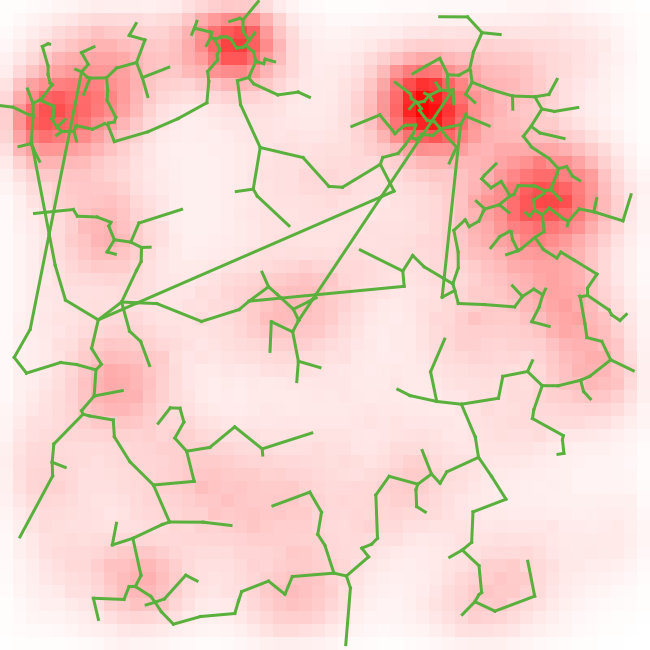
\includegraphics[width=\textwidth]{Figures/Cover/cover} \\ \vspace{0.5cm} % Picture

Présentée par\\
\spacedlowsmallcaps{\myName}\\ % Your name
\bigskip


%\mySubtitle \\ \medskip % Thesis subtitle
%Under the supervision of \myProf and \myOtherProf \\ \medskip
Sous la direction de \myProf et \myOtherProf \\ \medskip
%\myDegree \\
\myDepartment \\  \medskip
%\myFaculty \\  \bigskip
%\myUni \\ \bigskip

\bigskip

\myTime\ -- \myVersion % Time and version

\bigskip

Composition du Jury :

\noun{Arnaud Banos}, Directeur de Recherche, CNRS (Directeur)\\
\noun{Florent Le Néchet}, Maître de Conférence, Université Paris-Est (Directeur)\\

\vfill

\end{center}
\end{addmargin}

\end{titlepage} % Main title page

% Back of the title page

\thispagestyle{empty}

\hfill

\vfill

\noindent\myName: \textit{\myTitle,} \mySubtitle, %\myDegree, 
\textcopyright\ \myTime

% You may wish to do something with the back of the title page, such as including your supervisors, location or time frame of the work. Below is an example of doing so although you may want to tweak it to your liking.

%\bigskip

%\noindent\spacedlowsmallcaps{Supervisors}: \\
%\myProf \\
%\myOtherProf \\ 
%\mySupervisor

%\medskip \\

%\noindent\spacedlowsmallcaps{Location}: \\
%\myLocation

%\medskip \\

%\noindent\spacedlowsmallcaps{Time Frame}: \\
%\myTime
 % Back of the title page

\cleardoublepage% Dedication

\thispagestyle{empty}
\refstepcounter{dummy}

\pdfbookmark[1]{Dedication}{Dedication} % Bookmark name visible in a PDF viewer

\vspace*{3cm}



\bpar{
Our relation to our environment and people change at time scales we generally expect larger. Social relations are neither stationary nor in any kind of equilibrium at any time. They are chaos and complexity, as one's mind. As a witness, we include this preliminary dedication, for comparison purposes with the final version.
}{

}


%\begin{center}
%\emph{Ohana} means family. \\
%Family means nobody gets left behind, or forgotten. \\ \medskip
%--- Lilo \& Stitch    
%\end{center}
%
%\medskip
%
%\begin{center}
%Dedicated to the loving memory of Rudolf Miede. \\ \smallskip
%1939\,--\,2005
%\end{center} % Dedication page

\cleardoublepage% Abstract

%\renewcommand{\abstractname}{Abstract} % Uncomment to change the name of the abstract

\pdfbookmark[1]{Résumé}{Résumé} % Bookmark name visible in a PDF viewer

\begingroup
\let\clearpage\relax
\let\cleardoublepage\relax
\let\cleardoublepage\relax

%\chapter*{Abstract}{Résumé}
\chapter*{Résumé}
%Short summary of the contents\dots a great guide by 
%Kent Beck how to write good abstracts can be found here:  
%\begin{center}
%\url{https://plg.uwaterloo.ca/~migod/research/beckOOPSLA.html}
%\end{center}


La question récurrente de potentiels effets structurants des infrastructures de transports sur les territoires, est l'un des aspects de la problématique plus large des interactions entre réseaux et territoires. Celles-ci sont l'une des facettes de dynamiques territoriales complexes, au sein desquelles territoires et réseaux de transport seraient en co-évolution. L'objectif de cette thèse est de mettre à l'épreuve cette vision des interactions entre réseaux et territoires, autant sur le plan conceptuel qu'empirique, dans le but de l'intégrer au sein de modèles de simulation des systèmes territoriaux. La nature intrinsèquement multi-disciplinaire de la question nous conduit dans un premier temps à une analyse d'épistémologie quantitative, qui permet de dresser une carte du paysage scientifique et une description précise de la structure des différents modèles dans chaque discipline. La définition de la co-évolution et une méthode de caractérisation empirique, basée sur une analyse de correlations spatio-temporelles, est élaborée. Deux pistes complémentaires de modélisation, correspondant à des ontologies et des échelles différentes sont alors explorées. A l'échelle macroscopique, nous développons une famille de modèles dans la lignée des modèles d'interaction au sein des systèmes de villes développés par la Théorie Evolutive des Villes. Leur exploration montre qu'ils capturent effectivement des dynamiques de co-évolution, et leur calibration sur données démographiques pour le système de villes français (1830-1999) quantifie l'évolution des processus d'interaction comme l'effet tunnel ou le rôle de la centralité. A l'échelle mesoscopique, un modèle de morphogenèse capture la co-évolution de la forme urbaine et de la topologie du réseau. Il est calibré sur les indicateurs correspondants pour la forme et la topologie locales calculés pour l'ensemble de l'Europe. De multiples processus d'évolution du réseau (planification coût-bénéfices, rupture de potentiel, auto-organisation) sont montrés complémentaires pour produire l'ensemble des configurations réelles. La calibration est également faite au second ordre, c'est à dire sur les interactions entre indicateurs, pour lequel le modèle reproduit une grande diversité de situations existantes. Ces résultats suggèrent d'une part une construction théorique intégrant Théorie Evolutive Urbaine et Morphogenèse, et ouvrent d'autre part l'exploration d'une nouvelle génération de modèles urbains intégrant les dynamiques co-évolutives dans une perspective multi-échelles.




%-----------------------------------------------

\newpage

\cn{
\chapter*{建模交通网络和地域的共同演变 : 摘要}
}

\cn{运输基础设施对领土体系结构效应存在的问题远未得到解决。% La question de l'existence d'effets structurants des infrastructures de transports sur les systèmes territoriaux est loin d'être résolue. 
这是复杂的地域动态的一个方面,其中领土和交通网络正在共同演变。% C'est l'une des facettes de dynamiques territoriales complexes, au sein desquelles territoires et réseaux de transport sont en co-évolution.
这篇论文的目的是测试网络和地域之间的相互作用。%L'objectif de cette thèse est de mettre à l'épreuve cette vision des interactions entre réseaux et territoires.
它将在概念和经验上做到这一点,目的是将其整合到地域系统的模拟模型中。% Elle le fera autant sur le plan conceptuel que le plan empirique, dans le but de l'intégrer au sein de modèles de simulation des systèmes territoriaux.
我们正在处理的问题本质上是多学科的。% La problématique que nous traitons est intrinsèquement multi-disciplinaire.
出于这个原因,我们首先进行量化的认识论分析。% Pour cette raison, nous procédons dans un premier temps à une analyse d'épistémologie quantitative. 
它可以绘制科学的景观图,并精确地描述每个学科不同模型的结构。% Elle permet de dresser une carte du paysage scientifique et une description précise de la structure des différents modèles dans chaque discipline.
我们制定了一个共同进化的定义,并开发了一个基于时空相关分析的经验表征方法。% Nous élaborons une définition de la co-évolution et élaborons une méthode de caractérisation empirique basée sur une analyse de correlations spatio-temporelles.
探索两个互补的建模轨道。 它们对应于不同的本体和尺度。% Deux pistes complémentaires de modélisation sont explorées. Elles correspondent à des ontologies et des échelles différentes.
在宏观层面上,我们根据城市演变理论发展起来的城市体系内的相互作用模型发展了一个模型家族。% A l'échelle macroscopique, nous développons une famille de modèles dans la lignée des modèles d'interaction au sein des systèmes de villes développés par la Théorie Evolutive des Villes.
他们的探索表明,他们实际上捕捉到共同演化的动力。 他们对法国城市系统(1830-1999)的人口统计数据的校准量化了互动过程的演变。 这些例如是隧道效应或网络中心性的影响。% Leur exploration montre qu'ils capturent effectivement des dynamiques de co-évolution. Leur calibration sur données démographiques pour le système de villes français (1830-1999) quantifie l'évolution de processus d'interaction. Ceux-ci sont par exemple l'effet tunnel ou l'impact de la centralité dans le réseau.
在介观尺度上,形态演化模型捕捉城市形态和网络拓扑的共同演化。% A l'échelle mesoscopique, un modèle d'évolution morphologique capture la co-évolution de la forme urbaine et de la topologie du réseau.
根据整个欧洲计算的局部形态和拓扑结构的相应指标进行校准。% Il est calibré sur les indicateurs correspondants pour la forme et la topologie locales calculés pour l'ensemble de l'Europe.
网络演进的多个过程被考虑到:成本效益计划,潜在的突破,自组织。 它们似乎是互补的,可以产生所有的真实配置。% De multiples processus d'évolution du réseau sont pris en compte : planification coût-bénéfices, rupture de potentiel, auto-organisation. Ils apparaissent complémentaires pour produire l'ensemble des configurations réelles. 
校准也是按照第二顺序进行的,也就是指标之间的相互作用,模型重现了现有情况的多样性。% La calibration est également faite au second ordre, c'est à dire sur les interactions entre indicateurs, pour lequel le modèle reproduit une grande diversité de situations existantes.
这些结果一方面表明了把城市演变理论与形式演变相结合的理论建构。 另一方面,他们开辟了新一代城市模式的探索,这些模型将不得不整合多尺度协同进化动力学。% Ces résultats suggèrent d'une part une construction théorique intégrant Théorie Evolutive Urbaine et évolution de la forme. Ils ouvrent d'autre part l'exploration d'une nouvelle génération de modèles urbains qui devra intègre les dynamiques co-évolutives multi-échelles.
}





%-----------------------------------------------

\newpage

\chapter*{Abstract}











% old abstract

%Territorial systems exhibit complexity at any levels and for most of their aspects. Related disciplines \comment{(Florent) geography, planning, socio, economy}
%generally embrace complex systems science approaches to tackle their understanding and the associated dramatic \comment{(Florent)un peu fort ?}
%social and environmental issues. Choosing a specific angle of lecture of territories, \comment{(Florent)trop vite ds problématique, développer d'abord aspect dynamique}, idem
%it appears, following territorial theories of networks, that real networks play a crucial role in system dynamics, and in particular transportation networks. Taking furthermore a modeling paradigm, we ask to what extent a modeling approach to territorial systems as networked human territories can help disentangling complexly involved processes. We propose to build an associated theory, relying on a vision of human territories as networked, combined with the evolutive urban theory and insights from morphogenesis and co-evolution, that we call a \emph{theory of co-evolutive networked territorial systems}. \comment{(Florent) pas clair, pas forcément nommer}
% It is then embedded into a more general epistemological framework insisting on the notions of emergence and modularity. Quantitative epistemological analysis \comment{(Florent)trop précis}
% confirm the manual literature review and guide research towards co-evolutive models of networks and territories. We search for stylized facts in empirical datasets to also guide model construction. Methodological developments allow to expect information on dynamical processes from static correlations between urban morphology and network shape. The first modeling experiments include a calibrated spatial model of urban growth, giving an insight into theoretical assumption of network necessity. This model is then weakly coupled with a network generation heuristic to explore the space of feasible correlations. It paves the road for both comparison with real correlations and a strongly coupled calibrated model. We also explore novel paradigms such as the role of governance processes in network growth, through a game-theoretic agent-based model. These preliminary results provide the roadmap towards a family of comprehensive operational models of co-evolution between networks and territories that aim to disentangle their circular causalities.
%\comment{(Florent) trop de concepts dans l'abstract, peut pas apporter qqchse à tous}
%\comment{(Florent) commencer par expliquer ce que sont causalités circulaires et pourquoi difficiles à modéliser}
%\comment{(Arnaud) complexly : ?}
%\comment{(Arnaud) théorie des systèmes territoriaux en réseau co-évolutifs ?}





\endgroup			

\vfill % Abstract page



\cleardoublepage
% Abstract

%\renewcommand{\abstractname}{Abstract} % Uncomment to change the name of the abstract

%\pdfbookmark[1]{Reading Notes}{Reading Notes} % Bookmark name visible in a PDF viewer
\pdfbookmark[1]{Notes de Lecture}{Notes de Lecture}

\begingroup
\let\clearpage\relax
\let\cleardoublepage\relax
\let\cleardoublepage\relax

%\chapter*{Reading Notes}{Notes de Lecture}

\chapter*{Notes de Lecture}



Cette thèse devait initialement être rédigée en anglais pour sa version originale. Un premier tiers et la majorité des articles l'ont été, pour être repris et traduits par la suite, afin de répondre à une contrainte administrative d'un autre âge. Elle avait également été conçue comme une ``thèse à articles'', mais les fortes recommandations du CNU ont vite eu vent de cette ambition. Ainsi, la version courante est passée par maintes transformations et ``lissages'', afin de lui donner une forme, un fond et une identité ``classiques''. Nous nous excusons préalablement auprès du lecteur si des écueils de traduction ou d'articulation subsistent et perturbent la fluidité de la lecture.

L'ensemble des figures est produit par l'auteur, sauf la figure~\ref{fig:computation:xkcd} (source xkcd). La grande majorité des figures est \emph{directement} reproductible, c'est à dire pouvant être obtenue par execution des scripts. L'ensemble des codes sources, des modèles à l'interprétation des résultats et à cette propre rédaction, est disponible de manière ouverte avec l'ensemble de son historique atomique (\emph{commits}) sur le dépôt du projet\footnote{à \url{https://github.com/JusteRaimbault/CityNetwork}}. L'ensemble des jeux de données produits dans ce cadre est ouvert, et l'ensemble des données utilisées sont ouvertes ou rendues ouvertes (de manière agrégée correspondant au niveau d'utilisation par les modèles dans le cas d'une base tierce fermée).

Ce mémoire en lui-même a été relu par les lecteurs suivants (ordre alphabétique) : Arnaud Banos (AB), Florent Le Néchet (FL), Clémentine Cottineau (CC), dans l'esprit d'une revue ouverte : en suivant les commits successifs à \url{https://github.com/JusteRaimbault/ThesisMemoire}, l'utilisation de commandes spécifiques permet de retracer l'ensemble du processus de revue.



\endgroup			

\vfill







%\textit{Cette thèse est un voyage, tout d'abord géographique au travers des territoires très divers que nous visiterons tout autour du monde et dans des mondes qui n'existent pas. Un voyage entre des disciplines qui n'ont pas forcément l'habitude de se parler. Un voyage au delà des illusions et des idéaux naïfs sur une recherche qui serait surhumaine, un voyage initiatique dans la médiocrité quotidienne et l'étroitesse d'esprit, particulièrement dans ses relations à l'enseignement. Un trip sous drogues diverses qui aura cherché un sens jusqu'au bout pour comprendre que le sens du sens lui-même n'en avait pas. Une exploration préliminaire effleurant l'immensité des voyages qui nous attendent plus tard.}


 % Uncomment and create a Foreword.tex to include a foreword



\cleardoublepage% Publications - a page listing research articles written using content in the thesis

\pdfbookmark[1]{Publications}{Publications} % Bookmark name visible in a PDF viewer

\chapter*{Publications} % Publications page text

%Some ideas and figures have appeared previously in the following publications:\\

%\noindent Put your publications from the thesis here. The packages \texttt{multibib} or \texttt{bibtopic} etc. can be used to handle multiple different bibliographies in your document.

%\begin{refsection}[ownpubs]
%    \small
%    \nocite{*} % is local to to the enclosing refsection
%    \printbibliography[heading=none]
%\end{refsection}

%\emph{Attention}: This requires a separate run of \texttt{bibtex} for your \texttt{refsection}, \eg, \texttt{ClassicThesis1-blx} for this file. You might also use \texttt{biber} as the backend for \texttt{biblatex}. See also \url{http://tex.stackexchange.com/questions/128196/problem-with-refsection}.

\bpar{
The following works have an highly overlapping content with this thesis:
}{
Les travaux suivants contiennent une grande partie du contenu de cette thèse:
}

% NOTE : on self-plagiarism, be careful to precise when extract from a published paper : 
%  - http://academia.stackexchange.com/questions/12342/self-plagiarism-in-phd-thesis
%  - http://academia.stackexchange.com/questions/2029/can-i-use-the-work-in-my-journal-conference-publications-as-chapters-in-my-disse
%  - http://academia.stackexchange.com/questions/149/what-is-a-sandwich-thesis


\section*{Publications}{Publications}


\noindent Antelope, C., Hubatsch, L., Raimbault, J., and Serna, J. M. (2016). An interdisciplinary approach to morphogenesis. Forthcoming in Proceedings of Santa Fe Institute CSSS 2016.


\bigskip

\noindent Raimbault, J. (2017). A Discrepancy-Based Framework to Compare Robustness Between Multi-attribute Evaluations. In Complex Systems Design \& Management (pp. 141-154). Springer International Publishing. \cite{raimbault2016discrepancy}

\bigskip

\noindent Raimbault, J. (2016). Investigating the Empirical Existence of Static User Equilibrium, \textit{forthcoming in EWGT 2016 proceedings, Transportation Research Procedia.} arxiv:1608.05266 \cite{raimbault2016investigating}


\bigskip


\noindent Raimbault, J. (2016). Generation of Correlated Synthetic Data, forthcoming in \textit{Actes des Journ{\'e}es de Rochebrune 2016.}


\bigskip

\noindent Raimbault, J. (2015). Models Coupling Urban Growth and Transportation Network Growth: An Algorithmic Systematic Review Approach, forthcoming in \textit{ECTQG 2015 proceedings.} arxiv:1605.08888


\section*{Communications}{Communications}

\noindent Towards a Theory of Co-evolutive Networked Territorial Systems: Insights from Transportation Governance Modeling in Pearl River Delta, China, \textit{MEDIUM Seminar : Sustainable Development in Zhuhai, Guangzhou, Dec 2016.}


\bigskip


\noindent Models of growth for system of cities : Back to the simple, \textit{Conference on Complex Systems 2016, Amsterdam, Sep 2016.}



%Raimbault J., Bergeaud A. and Potiron Y. (2016). Investigating Patterns of Technological Innovation. \textit{Conference on Complex Systems 2016, Amsterdam, Sep 2016.}


\bigskip

\noindent For a Cautious Use of Big Data and Computation. \textit{Royal Geographical Society - Annual Conference 2016 - Session : Geocomputation, the Next 20 Years (1), London, Aug 2016.}


\bigskip

\noindent Indirect Bibliometrics by Complex Network Analysis. \textit{20e Anniversaire de Cybergeo, Paris, May 2016.}


\bigskip

\noindent Raimbault, J. \& Serra, H. (2016). Game-based Tools as Media to Transmit Freshwater Ecology Concepts, \textit{poster corner at SETAC 2016 (Nantes, May 2016).}


\bigskip

\noindent Le Néchet, F. \& Raimbault, J. (2015). Modeling the emergence of metropolitan transport authority in a polycentric urban region, \textit{ECTQG 2015, Bari, Sep 2015).}


\bigskip

\noindent Hybrid Modeling of a Bike-Sharing Transportation System, \textit{poster presented at ICCSS 2015, Helsinki, June 2015.}

\bigskip

\noindent Raimbault, J. \& Gonzales, J. (2015). Application de la Morphog{\'e}n{\`e}se de R{\'e}seaux Biologiques {\`a} la Conception Optimale d'Infrastructures de Transport, \textit{poster presented at Rencontres du Labex Dynamite, Paris, May 2015.}


 % Publications from the thesis page

%\cleardoublepage% Acknowledgements

%\pdfbookmark[1]{Acknowledgements}{Acknowledgements} % Bookmark name visible in a PDF viewer
\pdfbookmark[1]{Remerciements}{Remerciements}

%\begin{flushright}{\slshape    
%We have seen that computer programming is an art, \\ 
%because it applies accumulated knowledge to the world, \\ 
%because it requires skill and ingenuity, and especially \\
%because it produces objects of beauty.} \\ \medskip
%--- \defcitealias{knuth:1974}{Donald E. Knuth}\citetalias{knuth:1974} \citep{knuth:1974}
%\end{flushright}

%\bigskip

%----------------------------------------------------------------------------------------

\begingroup

\let\clearpage\relax
\let\cleardoublepage\relax
\let\cleardoublepage\relax

%\chapter*{Acknowledgements}
\chapter*{Remerciements}


% \textit{La forme et la fonction se produisent mutuellement de manière complexe. Des remerciements ne feraient pas partie du fond scientifique ? }

% grille

Un certain nombre de résultats obtenus dans cette thèse ont été calculés sur l'organisation virtuelle vo.complex-system.eu de l'European Grid Infrastructure (http://www.egi.eu). Nous remercions l'European Grid Infrastructure et ses National Grid Initiatives (France-Grilles en particulier) pour fournir le support technique et l'infrastructure. \\



% directeurs

% Ma profonde reconnaissance va naturellement en très grande partie à mes directeurs, qui ont rendu cette aventure possible et ont permis sa forme finale, par un pilotage subtil du système complexe que formait mes objets, mes modèles, mes idées. J'ai rencontré pour la première fois Arnaud Banos en octobre 2012 à l'ISC qu'il dirigeait, alors toujours rue Lhomond. C'était dans le cadre d'une supervision des \emph{Open Problems} du PA Systèmes Complexes, et nous nous étions immergés avec mon collègue Jorge dans le monde du multi-échelle, de l'optimisation multi-objectif, des réseaux biologiques auto-organisés (projet dont l'implémentation originale a d'ailleurs été reprise ici).


% Je tiens également à remercier Paul Bourgine et Kashayar Pakdaman











%%%%%%%%%%%
%% Invitation soutenance

% -> positionnement scientifique / impact potentiel

% personnalités scientifiques
% - A. Bonnafous
% - F. Laurent
% - N. Aveline
% - C. Rozenblat
% - L. D'Acci
% - D. Chavalarias
% - F. Varenne
% - F. Pfaender
% - D. Badariotti
% - L. Sanders
% - M. Barthelemy
% - J.P. Marchand
% - F. Durand-Dastès
% - P. Frankhauser


% SFICSS
% - European circ eco crew : Joris, Marius, Mario.
% - Matteo
% - Jelena

% LVMT
% -> annonce interne

% Geocités
% -> annonce interne

% ISC
% -> annonce interne

% EMCSS
% - Kashayar Pakdaman, René Doursat
% - anciens du master cs (via Mme Taki ?)
% - Carantino
% - Jorge

% CSSS2013
% - Claire, Nico


% X
% - Heliou(s), Buisson


% Ponts
% - Camille

% Medium
% - collègues Medium si en Europe
% - Elfie, Medhi

% Coauteurs
% (rq : // diagramme Clem : overlap avec potes etc)
% - Marion, Romain, Clem
% - Solène

% eleves
% ?


% potes
% - Anto, Yo (si en fr), Max, Arnaud
% - SFR
% - Axel
% - Hélène (et parents)
% - Cinzia
% - Solène, Charline


% autres
% - Hervé












\endgroup % Acknowledgements page

\pagestyle{scrheadings} % Show chapter titles as headings

\cleardoublepage% Table of Contents - List of Tables/Figures/Listings and Acronyms

\refstepcounter{dummy}

\pdfbookmark[1]{\contentsname}{tableofcontents} % Bookmark name visible in a PDF viewer

\setcounter{tocdepth}{1} % Depth of sections to include in the table of contents - currently up to subsections

\setcounter{secnumdepth}{2} % Depth of sections to number in the text itself - currently up to subsubsections

\manualmark
\markboth{\spacedlowsmallcaps{\contentsname}}{\spacedlowsmallcaps{\contentsname}}
\tableofcontents 
\automark[section]{chapter}
\renewcommand{\chaptermark}[1]{\markboth{\spacedlowsmallcaps{#1}}{\spacedlowsmallcaps{#1}}}
\renewcommand{\sectionmark}[1]{\markright{\thesection\enspace\spacedlowsmallcaps{#1}}}

\clearpage

\begingroup 
\let\clearpage\relax
\let\cleardoublepage\relax
\let\cleardoublepage\relax

%----------------------------------------------------------------------------------------
%	List of Figures
%----------------------------------------------------------------------------------------

\refstepcounter{dummy}
%\addcontentsline{toc}{chapter}{\listfigurename} % Uncomment if you would like the list of figures to appear in the table of contents
\pdfbookmark[1]{\listfigurename}{lof} % Bookmark name visible in a PDF viewer

\begin{adjustwidth*}{-1cm}{-2cm}

\listoffigures

\end{adjustwidth*}

\vspace{8ex}
%\newpage

%----------------------------------------------------------------------------------------
%	List of Tables
%----------------------------------------------------------------------------------------

\refstepcounter{dummy}
%\addcontentsline{toc}{chapter}{\listtablename} % Uncomment if you would like the list of tables to appear in the table of contents
\pdfbookmark[1]{\listtablename}{lot} % Bookmark name visible in a PDF viewer

%\chapter*{List of Tables}

\begin{adjustwidth*}{-1cm}{-2cm}

\phantomsection

\listoftables

\end{adjustwidth*}
        
\vspace{8ex}
\newpage
    
%----------------------------------------------------------------------------------------
%	List of Listings
%---------------------------------------------------------------------------------------- 

%\refstepcounter{dummy}
%\addcontentsline{toc}{chapter}{\lstlistlistingname} % Uncomment if you would like the list of listings to appear in the table of contents
%\pdfbookmark[1]{\lstlistlistingname}{lol} % Bookmark name visible in a PDF viewer

%\lstlistoflistings 

%\vspace{8ex}
%\newpage
       
%----------------------------------------------------------------------------------------
%	Acronyms
%----------------------------------------------------------------------------------------

%\refstepcounter{dummy}
%\addcontentsline{toc}{chapter}{Acronyms} % Uncomment if you would like the acronyms to appear in the table of contents
%\pdfbookmark[1]{Acronyms}{acronyms} % Bookmark name visible in a PDF viewer

%\markboth{\spacedlowsmallcaps{Acronyms}}{\spacedlowsmallcaps{Acronyms}}

%\chapter*{Acronyms}

%\begin{acronym}[ABM]
%\acro{ABM}{Agent-based Modeling}
%\acro{API}{Application Programming Interface}
%\acro{UML}{Unified Modeling Language}
%\end{acronym}  
             
             

%\begin{acronym}[SOC]
%\acro{ABM}{Self-organized Criticality}
%\end{acronym} 
             
             
             
                   
\endgroup % Contents, list of figures/tables/listings and acronyms

\cleardoublepage

\pagenumbering{arabic} % Arabic page numbering for thesis content (1, 2, 3, etc)
%\setcounter{page}{90} % Uncomment to manually start the page counter at an arbitrary value (for example if you wish to count the pre-content pages in the page count)

\cleardoublepage % Avoids problems with pdfbookmark

%----------------------------------------------------------------------------------------
%	THESIS CONTENT - CHAPTERS
%----------------------------------------------------------------------------------------






%%%%%%%%%%%%%%%%%%%%
%% Organisation and general points



\comment{(Florent) cf receuil articles du Monde sur Grd Paris (numériser)}

\comment{(Florent) HDR Anne ?}


\comment{(Florent) trop peu ancré concrètement dans le champ des interactions transport/ville - enchainement idée ok mais revoir granularité info. Catalogue de situations complexes d'interactions forme urbaine/transport à reproduire.}





%%%%%%%%%%%%%%%%%%%%
% TODO - todo
%
% -- TODO --

% - checker redondances bibliographie, et exactitude des records, publications arxiv, etc. !! biblio des appendices dans la générale ? a voir.
% - inclure éthique de la connaissance de Monod.
% - why not include artwork as appendix. science<->art (// poésies ?)
% - appendix : ecogeo - include results and discussions ; idem conf Medium ?
% - Morphogenesis : * reclarify link between dynamics and form in Thom's theory ; * find time to do quant epistemo ; * on the definition of the system and boundaries : missing part ?
% - somewhere clarification and discussion on definitions of emergence, Bedau etc. ? done on several points.
% - sur multi-scale modeling : who does some and how much ? à ajouter quelque part
% - pour la PDE : voir Villani, mentionner ?
% - effective dimension of urban system : sens ? (comment density) : question assez profonde à méditer - lié info sémantique portugali ? lié représentation minimale ?
% - on density multi-scale dvlpmt : pas clair ce que tu as en tête ici : je ne sais pas si tu auras le temps de creuser cela, mais pour du multi-scalaire, les schémas sont très aidant car c'est vite difficile à visualiser
% - morphogénétiques : est-ce que le mot existe, orthographe pas logique !
% - correlated synthetic data : appendix : inclure regressions
% - revoir discussion correlated synthetic data
% - aller interviewer JP Marchand (Theo Quant) (citation comprendre la co-évolution)
% - make tables uniform and clean
% - recompute indicators with capacity and/or hierarchy when possible with speed limits, to check how they change, and also correlations ? -> speeds pas assez fiables a priori ; fait toujours avec dans tous les cas
% - \cite{2015arXiv150600348A} : Enhanced Gravity Model, how to take better into account heterogeneous network topology, using entropy maximisation combined to gravity model. : a caser quelque part, ressemble sur le coupling, et gravité (sugg. intgib au début)

% - Knowledge framework : 
%    * portugali IRSSN dans la partie theory - conceptualisation.
%    * introduce necessary domains : at least of necessary domains, that we postulate these ones ; there may be an infinity  ?
%    * ajouter des éléments interview Clem.

% - Modelography : 
%    * tenter une classif endogène des modèles : selon les caractéristiques récupérées ? pas forcément pertinent vu taille des données
%    * processus extraction de manière ``synthétique'' : implique des catégories, des choix subjectif. ; idem région géographique : suppose une typologie de classement, niveaux etc. Both out of purpose for now.
%    * idem  pour modèles statistiques : conclusion sens causalité/signif. Travail plus poussé en lui-même. A Faire plus tard.
%

% - interviews : voir où inclure, selon quantité et contenu.

% - partie supplémentaire dans Modélographie : dissection précise des vrais modèles de coévolution ? (pas tant que ça).

% - (Arnaud) (sur le plan) : dans méthodo : ajouter Modèle agents - hors équilibre -> small part in review.

% - StaticCorrelations : 
%    * finir-choisir maps pour la Chine en annexe ; complémentaires celles Europe ?
%    * GWR pour échelle optimale.
%
% - CausalityRegimes : \cite{kasraian2010interaction} à caser dans les études stat ?
%
% - observation flottante : La disposition d'esprit peut être rapprochée de la philosophie -> zen ? pshychédélique ici ?

% - Macro exploration : explorer le Portugali ?

% - Macro application FR : base autoroutes ("data paper" en annexe ? -> penser à faire un vrai data paper avec Florent.)

% - (thematic 1.1.1) \comment{(Florent)pas besoin ni interet de se positionner sur emergence des societes} : si car lié à évolution culturelle, les villes comme étape de celle-ci : dans une perspective plus large (cf projet postdoc), fondamental.

% - (thematic 1.1.1) \comment{(Florent)Une strategie à adopter serait d'abord de decrire de facon basique, avec exemples concrets, la complexité des interactoins réseau/espace/settelements, puis de rappeler CS et proprietes, puis de decrire lesquelles de ces propriétés presentes dans ces interactions, lequelles modèles vont essayer de reproduire et pquoi.} -> le problème, comme le révèle la modelography et la biblio, puis les expériences de modélisation, trop vaste, notion coevol mal définie, peut d'info systématiques. la partie fondations fait partiellement ce travail, seulement après celle-ci on peut avoir une vision un peu plus claire. --  \comment{(Florent) TB mais en parler avant, c'est cela le coeur} (difficulté intrinsèque, réseau qui façonnent territoire)

% - Gaelle Lesteven Metro toulouse - thèse : http://confins.revues.org/7653 ; exemple postdoc ? pas publié a priori.



%% -- DONE --
%
%  X - attention aspect uniformisateur/limite totalitariste vision sci ? -> ok clarifier avec anarchisme et Feyerabend.
%  X - trouver un moyen d'élargir systématiquement toutes les figures ?

%%%%%%%%%%%%%%%%%%%%
% TODO - include notes

% -> notes.md




%%%%%%%%%%%%%%%%%%%%
% TODO - Reading Records
%
%% -- A LIRE -- 

% - lire Morin sur la pensée complexe
% - Moore Nature of Computation
% - (Arnaud) A LIRE : R Brunet, Discontinuités en géographie ; Pierre Dumolard (Espace Différencié) ; Guy DiMeo (L'homme, la société, l'espace)


%% -- A INCLURE --
%



%%%%%%%%%%%%%%%%%%%%
% TODO - Ideas

% - cours : la ville est la combinaison de forces opposées, souvent contradictoire. (cours analyse spatiale). far-from-equilibrium of course.

%  -- URGENT -- (when writing comments on network growth models) : do a sort of list of processes, implied objects, etc. / or a tab , from modeling, theories and CASES STUDIES --


% -  companion site à la Seb ?

% -  a note on open review via git ?



%%%%%%%%%%%%%%%%%%%%
% TODO - Citations
%
% -> potential citations

%  - Le sérieux n'est que la crasse accumulée dans les têtes vides - Roland Topor

%  - Science is an essentially anarchic enterprise - Paul Feyerabend, Against Method

%\headercit{Mais ce n'est pas une question d'{\^a}ge, de chiffres et de stats\\ Moi je te parle surtout de rage, de kif et d'espoir}{Youssoupha}{\textit{, Esperance de Vie}}

% %\headercit{Do or do not. There is no try.}{Yoda}{}

% %\headercit{We need to find Banos' tenth modeling law}{Ren{\'e} Doursat}{}

%%%%
% voie de garage

%  - % The Social Construction of What ?}{Ian Hacking}{\cite{hacking1999social} -> pas vraiment une citation, et pas adapté à grand chose..
 
%\headercit{Your theory is crazy, but not enough to be true.\comment{(Florent) rigolo mais le rapport avec le sujet est discutable}}{Niels Bohr}{}





%%%%%%%%%%%%%%%%%%%%
% TODO - Uncited
%
% -> uncited refs, why.
%
%2017arXiv170108673P -> number of states of HMM : ?
%levy1993t -> Levy theory on territory : need a deeper read and connections.
%pumain2017geography
%batty2017cities
%2017arXiv170107861D
%nicosia2009extending
%10.1371/journal.pone.0170830
%varma2017hpc
%Munafo:2017uq
%railsback2017
%2017arXiv170102973L
%2017arXiv170102383G
%shashok2017can
%miandoabchi2013multi
%farahani2013review
%fujita1982multiple
%bitbol2004autopoiesis
%dollens2014alan
%Chavalarias2016
%2016arXiv161208111S
%2016arXiv161208338T
%friesz1985transportation
%sui2004tobler
%miller2004tobler
%tobler2004first : Tobler giving precisions on the first law of geography
%2016arXiv161205463G
%raimbault2016discrepancy
%raimbault2016investigating
%2016arXiv161102269V
%2015arXiv150402550T
%batty2005agents
%xue2006spatial
%shen2002urban
%xu2005city
%10.1371/journal.pone.0166011
%10.1371/journal.pone.0166004
%2016arXiv161103232L
%hou2011transport
%cao2012accessibility
%huang2016association
%10.1371/journal.pone.0164553
%chan2005location
%tardy2004role
%perret2015roads
%makse1995modelling
%2016arXiv160904636V
%clauset2004finding
%2016arXiv160902000G
%2016arXiv160808839C
%Downey30082016
%osmosis
%xie2009topological
%rozenfeld2008laws
%2016arXiv160805770C
%2016arXiv160806313S
%2016arXiv160806897H
%2015arXiv151207603T
%duranton2007urban
%dimeo2016geographie
%2016arXiv160608103M
%raimbault2016generation
%raimbault2015hybrid
%raimbault2015user
%raimbault2016system
%swerts2013systemes
%swerts2015megacities
%florida2008rise
%hall1982great
%2016arXiv160805266R
%aveline2016medium
%lenechet:halshs-01272236
%2016arXiv160804472J
%ioannidis2005most
%2016arXiv160803608M
%batty2007creative
%chen2012wider
%hall1997modelling
%knowles2016sir
%reid2016decision
%carreira2000mode
%yu2012solving
%wang2015resilience
%masucci2014exploring
%fessel2012physarum
%gaughan2016spatiotemporal
%raimbault2016simpopsan
%10.1371/journal.pone.0160471
%10.1371/journal.pone.0159496
%pan2003croissance
%2016arXiv160708472M
%lyu2016developing
%emangard2009transports
%e18060197
%ishiguro1997bootstrapping
%Woodhouse19072016
%10.1371/journal.pone.0158826
%10.1371/journal.pcbi.1004947
%2016arXiv160703186A
%10.1371/journal.pone.0157261
%saichev2009theory
%karrer2011stochastic
%gastner2006shape
%10.1371/journal.pone.0157728
%2015arXiv150607608T
%2016arXiv160601959F
%sornette1997convergent
%solomon1996spontaneous
%gabaix2003theory
%newling1966urban
%bretagnolle2000long
%pumain2006villes
%okabe1987theoretical
%dellaposta2016endogenous
%Squartini:2013fk
%Takeuchi20153109
%2016arXiv160501949B
%klimek2012empirical
%10.1371/journal.pone.0154839
%2016arXiv160408816Z
%2016arXiv160407876G
%jiang2007topological
%akaike1998information
%heiss2008likelihood
%2005physics..12106P
%hall1990methodology
%burnham2004multimodel
%manning2014stanford
%thom1974stabilite
%benguigui1991suburban
%durand1990notion
%batty1991generating
%dauphine1995chaos
%dupuy:halshs-00438867
%damm1980response
%coffman1998railroad
%knight1977evidence
%goldberg1972evaluation
%alcaly1976transportation
%aveline2003ville
%2016arXiv160402872L
%2016arXiv160400758D
%2016arXiv160404155A
%2016arXiv160403904B
%2015arXiv151104268L
%echenique2012growing
%Brunton12042016
%banos2011christaller
%10.1371/journal.pone.0152686
%dupuy1993geographie
%newman1996land
%kenworthy2002transport
%tirnakli2015standard
%benettin1980lyapunov
%hijmans2015geographic
%10.1371/journal.pone.0151676
%offner2000territorial
%bourgine2010morphogenesis
%Fujita199693
%lenormand2015comparing
%soler2014calculating
%gallotti2015transportation
%krugman1998space
%lenormand2012generating
%decraene2013emergence
%varenne2008epistemologie
%derrible2010complexity
%10.1371/journal.pone.0150932
%10.1371/journal.pone.0148660
%le2015modeling
%mehaffy2007notes
%cuyala2013diffusion
%ciotti2015homophily
%el2006access
%2015arXiv151003797G
%2016arXiv160208451P
%choi2014patent
%shibata2008detecting
%zembri2010new
%2015arXiv150901940M
%schmid1994probabilistic
%noruzi2005google
%bohannon2014scientific
%2015arXiv150601280B
%2016arXiv160106075O
%10.1371/journal.pone.0147913
%barthelemy2015time
%raffestin1982remarques
%Gao:2016ty
%fujita1996economics
%2016arXiv160203774H
%blondel2008fast
%min2011real
%schultz2014random
%jedwab2013transportation
%offner2002x
%bitner2009complex
%raimbault2015models
%2015arXiv151205659M
%achlioptas2009explosive
%10.1371/journal.pone.0146491
%2015arXiv151207715C
%2015arXiv151205259R
%2015arXiv151200946S
%2015arXiv151201423W
%di1998espace
%2015arXiv151105468E
%2014arXiv1403.3005S
%Brummitt20150712
%beckman1996creating
%simini2012universal
%masucci2013gravity
%witten1981diffusion
%kuhnert2006scaling
%aghion2002schumpeterian
%andersson2002urban
%frankhauser1998fractal
%2015arXiv151006326H
%Sinatra:2015yu
%su2008effect
%fraedrich1986estimating
%chen2009spatial
%2015arXiv150909055P
%Perret:2015fk
%2015arXiv150907599C
%2015arXiv150803542B
%pumain2006hierarchy
%vattay2015quantum
%2014arXiv1403.7686B
%2015arXiv150904486M
%2015arXiv150903678R
%2015arXiv150905183R
%2015arXiv150905590H
%2015arXiv150904558J
%Pohlert:2015fk
%cheng2004notes
%cristelli2012there
%fox2005revisiting
%newman2005power
%clauset2009power
%kyriakidou2011applying
%bretagnolle:halshs-00159894
%sanders2006artificial
%courbaud2015applying
%2015arXiv150707878C
%10.1371/journal.pone.0133780
%gilli2005bassin
%servais2004polycentrisme
%leveque:halshs-00280396
%urbanek2011emdist
%wikle1999dimension
%galka2004solution
%vitanov2015test
%hens2015extreme
%2015arXiv150507372L
%pan2013urban
%tretyakov2011fast
%pumain2004urban
%Capozza1990187
%thevenin2013mapping
%schwartz2011spatial
%roth2012long
%10.1371/journal.pone.0029721
%Ye2014200
%donaldson2010railroads
%lucas1998mechanics
%moretti2004human
%banos2012network
%gauvin2009phase
%chen2010characterizing
%kang2012intra
%Karatzoglou:2004uq
%R-Core-Team:2015fk
%anderson1991turning
%underhill1990soviet
%baklanov2015projects
%perret2010multi
%crucitti2006centrality
%frankhauser2008fractal
%pumain1998urban
%Schwarz201029
%hebert2011structural
%batty2006hierarchy
%lugovoy2007analysis
%dorogovtsev2000structure
%pumain2002role : epistemology on TQG
%Mandelbrot1961198
%Mandelbrot195990
%bailey1999funk
%roopkumar2006generalized
%pumain2015multilevel
%reuillon2015
%10.1371/journal.pcbi.1004101
%anas1998urban
%ribeiro2010game
%Roumboutsos2008209
%le2010approche
%ordeshook1986game
%lenechet:halshs-00674059
%lenechet2012
%keitt2011rgdal
%baddeley2004spatstat
%gallego2010population
%hirtzel:tel-01121665
%martin2004generating
%abadie2011synth
%coulombel:tel-00601262
%strano2012elementary
%networkQgis
%mills2000thematic
%fujita2004new
%cookbookForR
%leurent2012disaggregate
%fields1999city
%dori2002object
%zeigler1989devs
%louail:tel-00584495
%goldspink2000modelling
%Liu201326
%lechner2006procedural
%parish2001procedural
%beauguitte2014r
%andersson2003urban
%brown2005spatial
%Magliocca2011183
%Ettema20111
%phan2010agent
%clarke1998loose
%He2006323
%kocabas2006coupling
%Kunz2000597
%zanette1997role
%clarke2007decade
%achibetmorphogenese
%rui2013urban
%lodin2011road
%porta2006network
%andersson2006complex
%eboli2012exploring
%duranton2012urban
%horner2012analyzing
%2013PhRvL.111s8702L
%antoni:hal-00914269
%berroir2005contribution
%guerois2002commune
%hall2006polycentric
%offner:halshs-00438903
%portugali2012complexity
%
%

% X biernacki2000assessing -> empirical likelihood (paper interactionGibrat)
% X bon2017novel -> SJS
% X bettencourt2007growth : Bettencourt scaling theory of cities
% X bourgine2010morphogenesis : in morphogenesis
% X loo1999development : planning transportation in DPR
% X favaro2007croissance : thèse JM Favaro
% X paulus2004coevolution : specialisation of urban areas










%\ctparttext{}





%%%%%%%%%%%%%%%%
%%  Introduction
%%%%%%%%%%%%%%%%


%% Contents
%
%    - General considerations on Complex Systems, positioning etc (thesis in cs science etc)
%    - Thematic introduction, geographical introduction of the subject.
%
%   - precisions on v1 memoire : foreword ?
%
%    - reading precisions : organisation, interdependances etc 
%
%   - reflexive aspect : here ?  


%\chapter*{Introduction}{Introduction}
\chapter*{Introduction}


% to have header for non-numbered introduction
\markboth{Introduction}{Introduction}


% -- citations on hold --
%\headercit{\bpar{It's when you shuffle the anthill that you get a touch of all its complexity.}{C'est quand on donne un coup de pied dans la fourmilière qu'on se rend compte de toute sa complexité.\comment[AB]{je persiste a dire que c'est oas une tres bonne idee !}\comment[FL]{Incipit de son directeur de these est maladroit}}
%}{Arnaud Banos}{}



\bigskip




%\bpar{
%``In consequence of a technical issue, traffic is interrupted on the line B of RER, for an unknown duration. More information will be given as soon as available''. There is a high probability that someone having lived or spent some time in the metropolitan region of Paris has already heard this frightening announce and endured the difficult consequences the rest of his day. But he might not be aware of the ramifications of causal cascades induced by this not-so-rare event. Territorial Systems, whatever the layers considered in their definitions, will always be extremely complex and interrelations at numerous temporal and spatial scales participate in the emergent behaviors observed at any levels of the system. Martin is a student who daily commutes from Paris to Palaiseau and will miss today a crucial exam, what will have a profound impact on his professional life : implications at a long time scale, small spatial scale and agent granularity. Yuangsi is connecting Orly and Roissy Airports, in his trip from London to Beijing, will miss his plane and his sister's wedding : large spatial scale, short time scale, agent granularity. A collective petition emerges from users, leading to new social organizational patterns and reaction from transportation authority that results in efforts to increase levels of service : mesoscopic temporal and spatial scale, swarm of agents granularity.
%}{
%``En conséquence d'un problème technique, le trafic est interrompu sur la ligne B du RER pour une durée indéterminée. Plus d'information seront fournies dès que possible''. Il y a des fortes chances pour que quiconque ayant vécu ou passé un peu de temps en région parisienne ait déjà entendu cette annonce glaçante et en ait subi les conséquences pour le reste de la journée. Mais il ne se doute sûrement pas des ramifications des cascades causales induites par cet évènement presque banal. Les systèmes territoriaux, quelles que soient les aspects considérés pour leur définition, ont une complexité croissante lorsqu'on augmente leur nombre, les interrelations à de nombreuses échelles spatiales et temporelles participant à la production des comportements émergents observés à tout niveau du système. Martin est un étudiant qui fait l'aller-retour journalier entre Paris et Palaiseau and manquera un examen crucial, ce qui aura un impact profond sur sa vie professionnelle : implications à une longue échelle de temps, une petite échelle spatiale et à la granularité de l'agent. Yuangxi était en train de relier les aéroports d'Orly et Roissy dans son voyage de Londres à Pékin et va manquer son avion ainsi que le mariage de sa soeur : grande échelle spatiale, courte échelle temporelle, granularité de l'agent. Une pétition collective émerge des voyageurs, conduisant à la création d'une organisation qui mettra la pression sur les autorités pour qu'elles augmentent le niveau de service : échelle temporelle et spatiales mesoscopique, granularité de l'aggregation d'agents.
%\comment[FL]{encore une fois : l'exemple mobilite quotidienne pour commencer me semble mal choisi}
%}


\bpar{}{

}



\bpar{
Looking for causes of the event will also lead to intricate processes at various scales, none of which seems to be a better explication than others : historical railway network in Parisian region shaped further extensions and RER B followed the former \textit{Ligne de Sceaux}, \noun{Delouvrier}'s schema for regional development, and its subsequent partial execution, are elements of explanation of structural weaknesses of Parisian public transportation network~\citep{gleyze2005vulnerabilite}; commuting patterns consequent to territorial organisation induce an overload of particular lines and thus a necessary increase in exploitation incidents. The list could be developed much longer and each approach related to an already mature scientific body of knowledge in different disciplines such as geography, urban economics, transportation. This amusing anecdote is enough to give a touch of the complexity of territorial systems. Our aim here is to dive into this complexity, and in particular to give an original insight into the study of relations between networks and territories. The choice of this reading position will be largely discussed in a further thematic part. Let for now concentrate on the originality of the point of view that we will take.
}{
La recherche de cause possible à l'incident conduira à des processus intriqués à diverses échelles, parmi lesquels aucun ne semble être une meilleure explication ; le développement historique du réseau ferroviaire en région parisienne a conditionné les évolutions futures et le RER B a suivi l'ancienne Ligne de Sceaux, le plan de \noun{Delouvrier} pour le développement régional et son execution partielle, sont également des éléments d'explication de la structure du réseau parisien de transports en commun qui conditionne la perturbation~\cite{gleyze2005vulnerabilite} ; les motifs pendulaires dus à l'organisation territoriale induisent une surcharge de certaines ligne et ainsi nécessairement une augmentation des incidents d'exploitation. La liste pourrait être ainsi continuée un certain temps, chaque approche apportant sa vision mature correspondant à un corpus de connaissances scientifiques dans des disciplines diverses comme la géographie, l'économie urbaine, les transports. Cette anecdote quotidienne est suffisante pour faire ressentir la complexité des systèmes territoriaux. Notre but ici est de se plonger dans cette complexité, et en particulier donner un point de vue original sur l'étude des relations entre réseaux de transport et territoires. Le choix de cette position sera largement discuté dans une partie thématique, nous nous concentrons à présent sur l'originalité du point de vue que nous allons prendre.
}





\section*{On General Positioning}{De la position générale}


\bpar{
\emph{The ambition of this thesis is to have no ambition.} Such an introduction, although seeming rash, contains at all levels the implicit logics behind our research process. At the first degree, we try as much as possible to take a exploratory and constructive approach, as much on theoretical and methodological domains than thematic domain, but also proto-methodological (tools applying the method) : if unidimensional or integrated ambitions should emerge, they would be conditioned to the arbitrary choice of a time sampling among the continuity of the dynamic that structures any research project. In the structural sense, the self-reference that underlines an apparent contradiction points out the centra aspect of reflexivity in our constructive approach, as much in the sense of the recursion of theoretical apparels, than for application of tools and methods developed to the work itself, or in the sense of the co-construction of the different approaches and of the different thematic axis. The processus of knowledge production can this way be read as a metaphor of studied processes. Finally, from a point of view closer to interpretation, it suggests the intention of a delicate position linking a political positioning which necessity is intrinsic to humanities (for example here against the technocratic application of models, or for the development of tools for an Open Science) with a rigor of objectivity coming more from other fields used, position that impose an increased prudence.
}
{
\emph{L'ambition de cette thèse est de ne pas avoir d'ambition.}
 Cette entrée en matière, rude en apparence, contient à différents niveaux les logiques sous-jacentes à notre processus de recherche. Au sens propre, nous nous plaçons tant que possible dans une démarche constructive et exploratoire, autant sur les plans théoriques et méthodologiques que thématique, mais encore proto-méthodologique (outils appliquant la méthode) : si des ambitions unidimensionnelles ou intégrées devaient émerger, elles seraient conditionnées par l'arbitraire choix d'un échantillon temporel parmi la continuité de la dynamique qui structure tout projet de recherche. Au sens structurel, l'auto-référence qui soulève une contradiction apparente met en exergue l'aspect central de la réflexivité dans notre démarche constructive, autant au sens de la récursivité des appareils théoriques, de celui de l'application des outils et méthodes développés au travail lui-même ou que de celui de la co-construction des différentes approches et des différents axes thématiques. Le processus de production de connaissance pourra ainsi être lu comme une métaphore des processus étudiés. Enfin, sur un plan plus enclin à l'interprétation, cela suggérera la volonté d'une position délicate liant une conscience politique dont la nécessité est intrinsèque aux sciences humaines (par exemple ici contre l'application technocratique des modèles, ou pour le développement d'outils luttant pour une science ouverte) à une rigueur d'objectivité plus propre aux autres champs abordés, position forçant à une prudence accrue.
}

%\comment[AB]{Déclaration discutable : si j’ai bien compris l’argumentaire, ton absence d’ambition tient 1) à l’absence de quête d’universalité (dépendance au contexte) et 2) à la dimension politique inhérente à ton objet. Je te ferais dire que 1) l’absence d’universalité n’est pas une tare (c’est même la norme en SHS) et 2) la dissociation science/politique ne tient plus la route depuis bien longtemps et ne concerne qu’un micro domaine des sciences les plus abstraites et théoriques (maths fondamentales, physique théorique peut-être,…what else ?)}[rq : logique proche de Morin - but contenu dans moyen ? - endogene.]



\section*{Scientific Context : Complexity Has Come of Age}{Contexte Scientifique : Paradigmes de la Complexité}


% \footnote{pour lesquels il n'existe pas de définition unifiée mais dont les champs d'application couvrent une étendue allant des neurosciences à la finance quantitative, en passant par exemple par la sociologie quantitative, la géographie quantitative, la biologie intégrative, etc.~\cite{newman2011complex}, et pour l'étude desquels diverses approches complémentaires peuvent être appliquées, comme les Systèmes Dynamiques, la Modélisation Basée Agent, la Théorie des Matrices Aléatoires}


\bpar{
To better introduce our subject, it is necessary to make the reader aware of the particular scientific context we are working in. It is necessary both to understand the general epistemology underlying research questions, and to be aware of the variety of methods and tools used. Contemporaneous science is progressively taking the shift of complexity in many fields.
That also implies an epistemological revolution to abandon strict reductionism that failed in most of its synthesis attempts~\cite{anderson1972more}. Arthur recently recalled~\cite{arthur2015complexity} that a mutation of methods and paradigms was also at stake by the increasing role of computational approaches replacing purely analytical techniques generally self-limited in their modeling and resolution scope. Capturing \emph{emergent properties} in models of complex systems is one of the ways to understand the essence of these new approaches.
}{
Pour une meilleure introduction du sujet, il est nécessaire d'insister sur le cadre scientifique dans lequel nous nous positionnons. Ce contexte est crucial à la fois pour comprendre les concepts épistémologiques implicites dans nos questions de recherche, et aussi pour être conscient de la variété de méthodes et outils utilisés. La science contemporaine prend progressivement le tournant de la complexité dans de nombreux champs que nous illustrerons par la suite, ce qui implique une mutation épistémologique pour abandonner le réductionnisme\footnote{De manière schématique, le réductionnisme consiste en la position épistémologique que les systèmes sont entièrement compréhensibles à partir des éléments fondamentaux les constituant et des lois régissant leur évolution. Les niveaux supérieurs n'ont ni autonomie ni pouvoirs causaux irréductibles.} strict qui a échoué dans la majorité de ses tentatives de synthèse~\cite{anderson1972more}. Arthur a rappelé récemment~\cite{arthur2015complexity} qu'une mutation des méthodes et paradigmes en était également un enjeu, de par la place grandissante prise par les approches computationnelles qui remplacent les résolutions purement analytiques généralement limitées en possibilités de modélisation et de résolution. La capture des \emph{propriétés émergentes} par des modèles de systèmes complexes est une des façons d'interpréter la philosophie de ces approaches.
}



\bpar{
These considerations are well known in Social Science (both quantitative and qualitative), in which the complexity of studied agents and systems is the justification of their existence : if humans were particles a whole branch of fields may have never emerged as thermodynamics would have solved most of social issues. \footnote{even if it would probably not have been the case as classical physics also failed in their attempts to include irreversibility and evolutions of Complex Adaptive Systems as Prigogine points out in \cite{prigogine1997end}} 
They are however less known nor accepted in more ``hard'' sciences such as physics : Laughlin develops in~\cite{laughlin2006different} a view of the discipline 
 at least as at a ``frontier of knowledge'' then other fields appearing as less mature. Most of knowledge is of classical nature although a majority of structures and systems would be \emph{self-organized}, what means that the single microscopic laws are not enough to determine macroscopic properties unless system evolution is simulated (more precisely this property can be taken as a definition of emergence on which we will come back further, and self-organization is intrinsically emergent). It corresponds to the first nightmare of Laplace's Deamon developed in~\cite{deffuant2015visions}.
}{
Ces considérations sont bien connues des Sciences Humaines et Sociales (qualitatives et quantitatives) pour lesquelles la complexité des agents et systèmes étudiés est une des justifications de leur existence : si les humains étaient effectivement des particules, on pourrait s'attendre à ce que la majorité des disciplines les prenant comme objet d'étude n'aient jamais émergé puisque la thermodynamique aurait alors résolu la majorité des problèmes sociaux\footnote{Bien que cette affirmation soit elle-même discutable, les sciences physiques classiques ayant également échoué à prendre en compte l'irréversibilité et l'évolution de Systèmes Complexes Adaptatifs comme le souligne~\cite{prigogine1997end}.}. Elles sont au contraire moins connues et acceptées en sciences ``dures'' comme la physique : \cite{laughlin2006different} développe une vision de la physique à la même position de ``frontière des connaissances'' que d'autre champs plus récents qui pourrait sembler en être encore à leur genèse. La plupart des connaissances actuelles concernent des structures classiques simples, alors qu'un grand nombre de systèmes présentent des propriétés \emph{d'auto-organisation}, au sens où les lois microscopiques ne sont pas suffisantes pour inférer les propriétés macroscopiques du système à moins que son évolution ne soit entièrement simulée (plus précisément cette vision peut être prise comme une définition de l'émergence sur laquelle nous reviendrons par la suite, or des propriétés auto-organisées sont par nature émergentes). Cela correspond au premier cauchemar du Démon de Laplace développé dans~\cite{deffuant2015visions}. 
} 


%-------------------------------------------------



\bpar{
As an informal mix of epistemological positions, methods, and fields of applications, \emph{Complexity Science} relies on typical paradigms such as the centrality of emergence and self-organization in most of phenomena of the real world, which make it lie on a frontier of knowledge closer of us than we can think (Laughlin, op.cit. ). Such concepts are indeed not new, as they were already enlighten by Anderson~\cite{anderson1972more}. Even cybernetics can be related to complexity by seing it as a bridge between technology and cognitive science~\cite{wiener1948cybernetics}.
}{
A la croisée de positionnements épistémologiques, de méthodes et de champs d'application, les \emph{Sciences de la complexité} se concentrent sur l'importance de l'émergence et de l'auto-organisation dans la plupart des phénomènes réel, ce qui les place plus proche de la frontière des connaissances que ce que l'on peut penser pour des disciplines classiques (\noun{Laughlin}, op. cit.). Ces concepts ne sont pas récents et avaient déjà été mis en valeur par~\cite{anderson1972more}. On peut aussi interpréter la Cybernétique comme un précurseur des Sciences de la Complexité en la lisant comme un pont entre technologie et sciences cognitives~\cite{wiener1948cybernetics}, et surtout en développant les notions de retroaction et de contrôle.
}

\bpar{
Later, synergetics~\cite{haken1980synergetics} paved the way for a theoretical approach of collective phenomena in physics. Reasons for the recent growth of works claiming a CS approach may be various. The explosion of computing power is surely one because of the central role of numerical simulations~\cite{varenne2010simulations}. They could also be the related epistemological progresses : apparition of the notion of perspectivism~\cite{giere2010scientific}, finer reflexions around the notion of model~\cite{varenne2013modeliser}\footnote{In that frame scientific and epistemological progress can not be dissociated and can be seen as coevolving}. The theoretical and empirical potentialities of such approaches play surely a role in their success\footnote{
Although the adoption of new scientific practices may be strongly biased by imitation and lack of originality~\cite{dirk1999measure}, or more ambivalent, by marketing strategies as the fight for funds is becoming a huge obstacle for research~\cite{bollen2014funding}.}, as confirmed in various domains of application (see~\cite{newman2011complex} for a general survey), as for example Network Science~\cite{barabasi2002linked} ; Neuroscience~\cite{koch1999complexity}; Social Sciences ; Geography~\cite{manson2001simplifying}\cite{pumain1997pour} ; Finance with the rising importance of econophysics~\cite{stanley1999econophysics} ; Ecology~\cite{grimm2005pattern}. The Complex Systems Roadmap~\cite{2009arXiv0907.2221B} proposed a double lecture of studies on Complex Systems : an horizontal approach connecting fields of study with transversal questions on theoretical foundations of complexity and empirical common stylized facts, and a vertical conceptions of disciplines, with the aim to construct integrated disciplines and corresponding multi-scale heterogeneous models. Interdisciplinarity is thus central in our scientific background.
}{
Plus tard, la Synergétique~\cite{haken1980synergetics} a posé les bases d'approches théoriques des phénomènes collectifs en physique. Les causes possibles de la croissance récente du nombre de travaux se réclamant d'approches complexes sont nombreuses. L'explosion de la puissance de calcul en est certainement une vu le rôle central que jouent les simulations numériques~\cite{varenne2010simulations}. Elles peuvent aussi être à chercher auprès de progrès en épistémologie : introduction de la notion de perspectivisme~\cite{giere2010scientific}, reflexions plus fine autour de la nature des modèles~\cite{varenne2013modeliser}\footnote{Dans ce cadre, les progrès scientifiques et épistémologiques ne peuvent pas être dissociés et peuvent être vus comme étant en co-évolution, au sens d'une forte interdépendance et d'une adaptation mutuelle.}. Les potentialités théoriques et empiriques de telles approchent jouent nécessairement un rôle dans leur succès\footnote{Même si l'adoption de nouvelles pratiques scientifiques peut par ailleurs être biaisé par l'imitation et le manque d'originalité~\cite{dirk1999measure}, ou de façon plus ambivalente, par des stratégies de positionnement indépendante des stratégies de connaissance, puisque le combat pour les fonds est un obstacle croissant à une recherche saine~\cite{bollen2014funding}.}, comme le confirme les domaines très variés d'application (voir~\cite{newman2011complex} pour une revue très générale), comme par exemple la Science de Réseaux~\cite{barabasi2002linked}; les Neurosciences~\cite{koch1999complexity}; les Sciences Humaines et Sociales,  dont la Géographie~\cite{manson2001simplifying}\cite{pumain1997pour}; la Finance avec les approches écononophysiques~\cite{stanley1999econophysics}; l'Ecologie~\cite{grimm2005pattern}. La Feuille de Route des Systèmes Complexes~\cite{2009arXiv0907.2221B} propose une double lecture des travaux en Complexité: une approche horizontale faisant la connexion entre champs d'étude par des questions transversales sur les fondations théoriques de la complexité et des faits stylisés empiriques communs, et une approche verticale, dans le but de construire des disciplines intégrées et les modèles multi-scalaires hétérogènes correspondants. L'interdisciplinarité est ainsi cruciale pour notre contexte scientifique.

}


\section*{Interdisciplinarity}{Interdisciplinarité}



\bpar{
We must further insist on the role of interdisciplinarity in the positions taken here. This is not a thesis in Geography nor in Complex Adaptive Systems Modeling,
 but in \emph{Complex Systems Science} that we claim as a proper discipline following \noun{Paul Bourgine}.
  It will naturally be seen with defiance by scholars of various concerned disciplines, as recent examples of misunderstandings and conflicts have illustrated~\cite{dupuy2015sciences}.
}{
Il est important d'insister sur le rôle de l'interdisciplinarité dans la position de recherche prise ici. Il s'agit autant d'un travail en Géographie Théorique et Quantitative qu'en Modélisation de Systèmes Complexes, étant finalement les deux à la fois selon le point de vue que prendra le lecteur. En ce sens, nous le réclamons de la \emph{Science des Systèmes Complexes} que nous tenterons de positionner comme discipline propre à travers cette implémentation précise\footnote{Un niveau de lecture abstrait du travail dans son ensemble apportera des informations sur la production de connaissance elle-même, comme nous le développerons en~\ref{sec:knowledgeframework}.}. Ce n'est pas sans risques d'être lu avec méfiance voir défiance par les tenants des disciplines classiques, comme des exemples récents de malentendus ou conflits ont récemment illustré~\cite{dupuy2015sciences}. Il faut se rappeler l'importance de la spirale vertueuse de \noun{Banos} entre disciplinarité et interdisciplinarité~\cite{banos2013pour}. Celle-ci doit nécessairement impliquer différents agents scientifiques, et il est compliqué pour un agent de se positionner dans les deux branches ; notre fond scientifique devra nous permettre de ne pas de nous positionner uniquement dans la \emph{disciplinarité géographique} (même si celle-ci sera simultanément une composante cruciale) mais bien aussi dans celle des Systèmes Complexes (qui est interdisciplinaire, voir~\ref{sec:epistemology} pour contourner la contradiction apparente), et notre sensibilité scientifique et épistémologique nous pousse à faire de même.
}

% rq : point de vue = grille de lecture
% \comment[AB]{je trouve que tu abandonnes bien vite la partie. Pourquoi renoncer dès le début alors que tu pourrais laisser la liberté à celui/celle qui te lit de décider si c’est AUSSI de la géo ou non ?}

\bpar{
The positioning of \noun{Batty} proposing \textit{A new Science of Cities}~\cite{batty2013new} (that he subtly presents as \textit{The} new science of cities) is directed towards an integration of disciplines and methods into a science defined by its object of study, cities.
Its theoretical and epistemological weaknesses (no theoretical constructions of studied geographical objects on the one hand, approximative contextualization of complexity) combined with an overall impression of \emph{pot-pourri} of forgotten works
 (space syntax, land-use models), unfortunately avoid us to use it as we will use geographical theories (e.g. evolutive urban theory) in an appropriated epistemological complexity context. Yet our reading of this work may be the result of a misunderstanding due to different cultural backgrounds.
}
{
Le positionnement de \noun{Batty} lorsqu'il propose \textit{Une Nouvelle Science des Villes}~\cite{batty2013new} %(qu'il présente avec humour comme \textit{La} nouvelle science des villes)
, se présente comme une intégration des disciplines et méthodes vers une science définie par son objet d'étude, les villes.
%Its theoretical and epistemological weaknesses (no theoretical constructions of studied geographical objects on the one hand, approximative contextualization of complexity) combined with an overall impression of \emph{pot-pourri} of forgotten works (space syntax, land-use models), unfortunately avoid us to use it as we will use geographical theories (e.g. evolutive urban theory) in an appropriated epistemological complexity context.  Yet our reading of this work may be the result of a misunderstanding due to different cultural backgrounds. \comment[Arnaud]{j'espère que tu abuses ? :) !! Argument d'autorité}[yes, changer positionnement complètement malvenu] \comment[Florent]{attention arguments autorité ; insister sur difficulté à intégrer paradigmes plutot que juger précédents}[idem]
}




\bpar{
The scientific evolution of complexity that some see as a revolution~\cite{colander2003complexity}, or even as \emph{a new kind of science}~\cite{wolfram2002new}, could indeed face intrinsic difficulties due to behaviors and a-priori of researchers as human beings.
 More precisely, the need of interdisciplinarity that makes the strength of Complexity Science may be one of its greatest weaknesses, since the highly partitioned structure of science organization has sometimes negative impacts on works involving different disciplines. We do not tackle the issue of over-publication, competition, indexes, which is more linked to a question of open science and its ethics, also of high importance but of an other nature. That barrier we are dealing with and we might struggle to triumph of, is the impact of certains \emph{cultural disciplinary differences} and out-coming conflicts on views and approaches. 
The drama of scientific misunderstandings is that they can indeed annihilate progresses by interpreting as a falsification some work that answers to a totally different question. The example of a recent work on top-income inequalities given in~\cite{aghion2015innovation}, which conclusions are presented as opposed from the one obtained by Piketty~\cite{piketty2013capital}, follows such a scheme. Whereas Piketty focused on constructing long-time clean databases for income data and showed empirically a recent acceleration of income inequalities, his simple model aiming to link this stylized fact with the accumulation of capital has been criticized as oversimplified. On the other hand, Bergeaud \textit{et al.} prove by a model of innovation economics that \emph{under certain assumptions} income gaps may be beneficial to innovation and consequently a general utility. Thus diverging conclusions about the role of personal capitals in the economy.
But diverging \emph{views} or \emph{interpretations} does not mean a scientific incompatibility, and one could imagine try to gather both approaches in an unified framework and model, yielding possibly similar or different interpretations. This integrated approach has chances to contain more information (depending on how coupling is done) and to be a further advance in Science. In an other but similar vein, \cite{2017arXiv170105627H} reanalyses biological data from a 1943 experiment that claimed to rule out Lamarckian over Darwinian evolution processes, and show that the conclusion are wrong in the current Data analysis (enormous advances in theoretical and processing techniques) and scientific context (with numerous other proofs today of Darwinian processes) : this is a good example of a context-misunderstanding and how conclusions strongly depend on both technical and thematic frameworks. We shall now briefly develop other examples to give an overview how conflicts between disciplines can be damaging.
}{
L'évolution scientifique des sciences de la complexité, qui est vue par certains comme une révolution~\cite{colander2003complexity}, ou même comme \emph{un nouveau type de science}~\cite{wolfram2002new}, pourrait affronter des difficultés intrinsèques dues aux comportements et a-priori des chercheurs en tant qu'être humains. Plus précisément, le besoin d'interdisciplinarité qui fait la force des Sciences de la Complexité pourrait devenir une de ses grandes faiblesses, puisque la structure fortement en silo de la science peut avoir des impacts négatifs sur les initiatives impliquant des disciplines variées. Nous n'évoquons pas les problèmes de sur-publication, quantification, competition, qui sont plus liés à des questions de Science Ouverte et de son éthique, tout aussi de grande importance mais d'une autre nature. Cette barrière qui nous hante et que nous pourrions ne pas surmonter, a pour plus évident symptôme des \emph{divergences culturelles disciplinaires}, et les conflits d'opinion en résultant. Ce drame du malentendu scientifique est d'autant plus grave qu'il peut en effet détruire totalement certains progrès en interprétant comme une falsification des travaux qui traitent une question toute différente. L'exemple récent en économie d'un travail sur les inégalités liées aux hauts revenus présenté dans~\cite{aghion2015innovation}, et dont les conclusions ont été commentées comme s'opposant aux thèses de~\cite{piketty2013capital}, est typique de ce schéma. Ce second se concentre sur la construction de bases de données propres sur le temps long pour les revenus et montre empiriquement une récente accélération des inégalités de revenus, son modèle visant à lier ce fait stylisé avec l'accumulation de capital a été critiqué comme trop simpliste. D'autre part, \cite{aghion2015innovation} montrent par des analyses économétriques que s'il existe bien un lien de causalité de l'innovation vers les inégalités de haut salaires, l'innovation accroit cependant la mobilité sociale, étant donc également moteur de réduction des inégalités. D'où des conclusions divergentes sur le rôles des capitaux personnels dans une économie, notamment sur leur relation ambigüe à l'innovation. Mais des \emph{point de vue} ou \emph{interprétations} différentes ne signifient pas une incompatibilité scientifique, et on pourrait même imaginer rassembler ces deux approches dans un cadre et modèle unifié, produisant des interprétations possiblement similaires et potentiellement encore nouvelles. Une telle approche intégrée aura de grandes chances de contenir plus d'information (selon la façon dont le couplage est opéré) et être une avancée scientifique. Cette expérience de pensée illustre les potentialités et la nécessité de l'interdisciplinarité. Dans une autre veine assez similaire, \cite{2017arXiv170105627H} ré-analyse des données biologiques d'une expérience de 1943 qui prétendait confirmer l'hypothèse des processus d'évolution Darwiniens par rapport aux processus Lamarckiens, et montrent que les conclusions ne tiennent plus dans le contexte actuel d'analyse de données (avances énormes sur la théorie et les possibilités de traitement) et scientifique (avec d'autres nombreuses preuves de nos jours des processus Darwiniens) : c'est un bon exemple de malentendu sur le contexte, et la manière selon laquelle le cadre de travail à la fois technique et thématique influence fortement les conclusions scientifiques. Nous développons à présent divers exemples révélateurs de la manière dont des conflits entre disciplines peuvent être dommageables.
}

%\comment[AB]{tout ceci remet en question ton « absence d’ambition » me semble-t-il}[par l'amplitude disciplinaire recherchée tu veux dire ?]

%\paragraph{Physics reinvents geography}{La tentation de réinventer la géographie}


\bpar{
As already mentioned, \noun{Dupuy} and \noun{Benguigui} points out in \cite{dupuy2015sciences} the fact that urban sciences
 have recently known open conflicts between old tenants of the disciplines and new arrivants, especially physicists.
 The availability of large datasets of new type of data (social networks, ICT data) have drawn their attention towards the study of objects traditionally studied by human science, as analytical and computational methods of statistical physics became applicable. Although these studies are generally presented as the construction of a scientific approach to cities, implying that existing knowledge was not scientific because of their more qualitative aspect, they have not unveil specifically novel knowledge on urban systems : 
  to give some examples, \cite{barthelemy2013self} concludes that Paris has followed a transition during Haussman period and that the evolution of a city is the combination of local transformations and global planning operations, what are facts known for a long time in urban history and urban geography. \comment{(Florent) qui a découvert avant ?}
  \cite{chen2009urban} rediscovers that the gravity model can be improved by adding lags in interactions and theoretically derives the expression of the force of interaction between cities, without any thematic theoretical background. Examples could be multiplied, confirming the current discomfort in communication between physicists and urban geographers. Significant benefices could results from a wise integration of disciplines~\cite{o2015physicists} but the road seems still long. 
}{
Comme déjà mentionné, \noun{Dupuy} et \noun{Benguigui} soulignent dans~\cite{dupuy2015sciences} le fait que dans le domaine de l'urbanisme, ont récemment éclaté des conflits ouverts entre les tenants classiques des disciplines et des nouveaux arrivants, en particulier les physiciens, même si leur entrée dans le domaine n'est pas nouvelle. La disponibilité de grand jeux de données d'un nouveau type (réseaux sociaux, données des nouvelles technologies de la communication) ont attiré l'attention d'un plus grand nombre sur des objets plus traditionnellement étudiés par les sciences humaines, puisque les méthodes analytiques et computationnelles de la physique statistique sont devenues applicables. Bien que ces travaux soient généralement présentés comme la construction d'une approche scientifique des villes, tout en discutant la nature scientifique des approches existantes, la nouveauté réelle des résultats obtenus et la non-légitimation des approches ``classiques'' sont discutables. Pour citer quelques exemples, \cite{barthelemy2013self} conclut que Paris a subit une transition pendant la période d'Haussman et ses opérations de planification globale, qui sont des faits naturellement connus depuis longtemps en Histoire Urbaine et Géographie Urbaine. \cite{chen2009urban} redécouvre que le modèle gravitaire est amélioré par l'introduction de décalages dans les interactions et dérive analytiquement l'expression d'une force d'interaction entre les villes, sans se placer dans un cadre théorique ou thématique. De tels exemples peuvent être multipliés, confirmant l'inconfort courant entre physiciens et géographes. Des bénéfices significatifs pourraient résulter d'une intégration raisonnée des disciplines~\cite{o2015physicists} mais la route semble être bien longue encore.
}


%\paragraph{Economic Geography or Geographical Economics ?}{Economie Géographie ou Géographie Economique ?}


\bpar{
Similar conflict occurred in economics : as \cite{marchionni2004geographical} describes, the discipline of economic geography, traditionally close from geography, heavily criticized a new stream of thought named \emph{geographical economics}, which purposes is spatialization of mainstream economic techniques. Both do not have the same purposes and aims, and the conflict appears as a total misunderstanding for an external observer.
}{
Des conflits similaires se rencontrent à l'interface des relations entre économie et géographie : comme le décrit \cite{marchionni2004geographical}, la discipline de la géographique économique, traditionnellement proche de la géographie, a fortement critiqué à son émergence l'approche relativement récente \emph{Nouvelle Economie Géographique}. Celle-ci provient de l'économie et son but est la prise en compte de l'espace par les méthodes économiques classiques. Elles n'ont en fait pas les mêmes desseins et buts, et le conflit apparaît comme un malentendu complet vu d'un oeil extérieur. Par exemple, la Nouvelle Economie Géographique privilégiera des explications impliquant des processus économiques universels et indépendant des échelles, tandis que la Géographie Economique basera son argumentation sur les particularité locales et la contingence des processus. Les hypothèses épistémologiques sous-jacentes sont également très différentes, comme par exemple la relation au réalisme, la première étant fondée sur un réalisme abstrait pas forcément concrètement réaliste (utilisation de processus abstraits), tandis que la deuxième sera plus pragmatique. La mesure dans laquelle ces deux approches sont complémentaires ou incompatible reste toutefois une question ouverte d'après \cite{marchionni2004geographical}. Des relations disciplinaires similaires seront rencontrées dans notre travail, comme entre la physique et la géographie. Nous développons par ailleurs en~\ref{app:sec:ecogeo} une exploration des liens entre économie et  géographie du point de vue de la modélisation.
}



%\paragraph{Agent-based Modeling in Economy}{Modélisation basée agent en Economie}


\bpar{
Disciplinary conflicts may also manifest themselves as the reject of novel methods by mainstream currents. Following \cite{farmer2009economy}, the operational failure of most classic economic approaches could be compensated by a broader use of agent-based modeling and simulation practices. The lack of analytical framework that is natural in the study of complex adaptive systems seems to be rebutting for most of economists.
}{
Des conflits disciplinaires peuvent aussi se manifester sous la forme d'un rejet de méthodes nouvelles par les courants dominants. Suivant \noun{Farmer}~\cite{farmer2009economy}, l'échec opérationnel de la plupart des approches économiques classiques pourrait être compensé par un usage plus systématique de la modélisation et simulation basées agent. L'absence de résolution analytique qui est inévitable pour l'étude de la plupart des systèmes complexes adaptatifs semble rebuter la plupart des économistes. Or, \cite{barthelemy2016structure} insiste sur la déconnexion exacerbée entre une grande partie des modèles et théories économiques et les observations empiriques, du moins dans le domaine de l'économie urbaine. Celle-ci pourrait être un symptôme de la déconnexion disciplinaire évoquée ci-dessus. Toujours en économie, \cite{storper2009rethinking} propose aussi des changements de paradigmes par un retour à l'agent et une construction associée de théories \emph{evidence-based}.
}


%\paragraph{Finance}{Finance}

\bpar{
In Quantitative Finance coexist various stream of research with a very few interactions. Let consider two examples. On the one hand, Statistics are highly advanced in theoretical mathematics, using stochastic calculus and probabilities to obtain very refined estimators of parameters for a given model (see e.g. \cite{barndorff2011multivariate}). On the other hand, Econophysics aims to study empirical stylized facts and infer empirical laws to explain complexity-related phenomena in financial systems~\cite{stanley1999econophysics}, such as e.g. cascades leading to market crashes, fractal properties of asset signals, complex structure of correlation networks. Both have their advantages in a particular context and each would benefit from increased interactions between the fields.
}{
La finance quantitative peut être instructive pour notre propos et sujet, d'une part par les similarités de la cuisine interdisciplinaire avec notre domaine (rapport avec la physique et l'économie, champs plus ou moins ``rigoureux'', etc.). Dans ce domaine coexistent divers champs de recherche ayant très peu d'interactions entre eux. On peut considérer deux exemples. D'une part, les statistiques et l'économétrie sont extrêmement avancées en mathématiques théoriques, utilisant par exemple des méthodes de calcul stochastique et de théorie des probabilité pour obtenir des estimateurs très raffinés de paramètres pour un modèle donné (voir par exemple \cite{barndorff2011multivariate}). D'autre part, l'éconophysique a pour but d'étudier des faits stylisés empiriques et inférer les lois correspondantes pour tenter d'expliquer des phénomènes économiques, par exemple ceux liés à la complexité des marchés financiers~\cite{stanley1999econophysics}. Ceux-ci incluent les cascades menant aux ruptures de marché, les propriétés fractales des signaux des actifs, la structure complexe des réseaux de corrélation. Chacun a ses avantages dans un contexte particulier et gagnerait à des interactions accrues entre les deux domaines.
}


\bpar{
These diverse examples illustrate how interdisciplinarity is both crucial and difficult to achieve. We will try to follow that narrow path in our work, borrowing ideas, theories and methods from various disciplines, aiming for the construction of an integrated knowledge. Indeed, coupling heterogeneous approaches at different levels and scales 
will be a cornerstone of our thesis, skeleton of the underlying philosophy and building brick of the theory we will propose.
}{
Ces divers exemples pris au fil du vent sont de brèves illustrations du caractère crucial de l'interdisciplinarité et de sa difficulté à pratiquer. Sans presque exagérer, on pourrait imaginer l'ensemble des chercheurs se plaindre de mauvaises ou difficiles expériences d'interdisciplinarité, avec un retour largement positif lors des rares succès. Nous allons tenter par la suite d'emprunter ce chemin étroit, empruntant des idées, théories et méthodes de diverse disciplines, dans l'idéal de la construction d'une connaissance intégrée.
}


%\comment[JR]{également un développement sur ``quanti-quali'' ?}
% pas besoin : en ouverture avec domaines connaissance a la fin.






%-------------------------------------------------

\section*{Complexity in Geography}{Paradigmes de la Complexité en Géographie}


\comment[FL]{la partie ``paradigmes de la complexite en geographie'' fait un peu ``name-dropping'' $\rightarrow$ quels points clés de cette litterature dans ta problematique ?}


\bpar{
Coming back to our introducing anecdote, we will focus on our thematic object of study that are territorial systems.
 More generally, we propose an overview of the role of complexity in geography. Geographers are familiar with complexity for a long time, as the study of spatial interactions is one of its purposes. The variety of fields in geography (geomorphology, physical geography, environmental geography, human geography, health geography to give a few) has certainly been important in the subtlety of the geographical thinking, that considers heterogeneous and multi-scalar processes.
}{
Pour revenir à notre anecdote introductive, nous nous concentrons sur l'étude d'un objet thématique qui sera les systèmes territoriaux : à l'échelle microscopique, les agents peuvent bien être vus comme éléments constitutifs fondamentaux du territoire, qui émergera comme processus complexe à différentes échelles. Plus généralement, il s'agit par commencer de brosser une revue du rôle de la complexité en géographie. Les géographes sont naturellement familiers avec la complexité, puisque l'étude des interactions spatiales est l'un de leurs objets de prédilection. La variété de champs en géographie (géomorphologie, géographie physique, géographie environnementale, géographie humaine, géographie de la santé, etc. pour en nommer quelques) a sûrement joué un rôle clé dans la constitution d'une pensée géographique subtile, qui considère des processus hétérogènes et multi-scalaires.
}



\bpar{
\noun{Pumain} recalls in~\cite{pumain2003approche} a subjective history of the emergence of complexity paradigms in geography. Cybernetics yielded system theories as the one developed by Forrester.
 Later the shift to self-organized criticality and self-organisation concepts in physics conducted to corresponding developments in geography, as \cite{sanders1992systeme} witnesses the application of the concepts of synergetics for the dynamics of an urban system. Finally, Complex Systems paradigms as we currently know them appeared from various points of view. For example, the fractal nature of urban shape was introduced in~\cite{batty1994fractal} and had numerous application including more recent developments~\cite{keersmaecker2003using}. \noun{Batty} also introduced cellular automata in urban modeling and proposed a joint synthesis with agent-based modeling and fractals in~\cite{batty2007cities}.
}{
\noun{Pumain} rappelle dans~\cite{pumain2003approche} une histoire subjective de l'émergence des paradigmes de la complexité en géographie. La cybernétique a produit des théories des systèmes comme celle utilisée pour les premiers modèles de dynamique des systèmes visant à simuler l'évolution de variables caractérisant un territoire, sous la forme d'équations différentielles couplées, comme \cite{chamussy1984dynamique} l'illustre pour un modèle couplant population, emplois et stock de logements. Plus tard, le glissement vers les concepts de criticalité auto-organisée et d'auto-organisation en physique ont conduit aux développements correspondants en géographie, comme~\cite{sanders1992systeme} qui témoigne de l'application des concepts de la synergétique aux dynamiques des systèmes urbains. Enfin, les paradigmes actuels des systèmes complexes ont été introduits par plusieurs entrées. Par exemple, l'étude de la nature fractale de la forme urbaine a été introduite par~\cite{batty1986fractal}, plus tard synthétisée par~\cite{batty1994fractal} et a eu de nombreuses applications jusqu'à des développements plus récents comme~\cite{keersmaecker2003using}.
%\comment{lier avec les approches de Frankhauser} citer  http://www.persee.fr/doc/spgeo\_0046-2497\_1990\_num\_19\_1\_2943 ?
Les automates cellulaires, introduits en géographie par \noun{Tobler}~\cite{couclelis1985cellular}, sont une autre entrée des approches complexes pour la modélisation urbaine. \noun{Batty} en propose une synthèse jointe avec les modèles basés agents et les fractales dans~\cite{batty2007cities}. 
}


\bpar{
}{
Relativement récemment, la Théorie du \emph{Scaling} a été importée de la biologie et des relations allométriques pour expliquer les lois d'échelle urbaine comme propriétés universelles liées au type d'activité : infrastructure et économies d'agglomération (scaling infralinéaire) ou résultante d'un processus d'interactions sociales (scaling supralinéaire), et suppose les villes comme versions à l'échelle l'une de l'autre~\cite{bettencourt2007growth}.
}




\bpar{
 An other incursion of complexity in geography was for the case of urban systems through the evolutive urban theory of \noun{Pumain}. In close relation with modeling from the beginning (the first Simpop model described in~\cite{sanders1997simpop} enters the theoretical framework of \cite{pumain1997pour}), this theory aims to understand system of cities as systems of co-evolving adaptive agents, interacting in many ways, with particular features emphasized such as the diffusion of innovation. The series of Simpop models~\cite{pumain2012multi} focused in testing various assumptions of the theory.
 For example, different underlying mechanisms were revealed for european city systems and city system of the united states~\cite{bretagnolle2010comparer}. At other time scales and in other contexts, the SimpopLocal model~\cite{schmitt2014modelisation} aimed to investigate the conditions for the emergence of hierarchical urban systems from disparate settlements. A minimal model (in the sense of sufficient and necessary parameter) has been isolated thanks to the use of intensive computation with the model exploration software OpenMole~\cite{schmitt2014half}, what was a result analytically not derivable for this kind of complex model. The technical progresses of OpenMole~\cite{reuillon2013openmole} were done simultaneously with theoretical and empirical advancements. Epistemological advances were also essential to this framework, as \noun{Rey} develops in~\cite{rey2015plateforme}, and novel concepts such as incremental modeling~\cite{cottineau2015incremental} were found, with powerful concrete applications : \cite{cottineau2014evolution} implemented it on the soviet city system and isolated dominating socio-economic processes, by systematic testing of thematic assumptions and implementation functions. Directions for the development of such Modeling and Simulation practices in quantitative geography were recently introduced by \noun{Banos} in~\cite{banos2013pour}. He concludes with nine principles\footnote{I remember \noun{Ren{\'e} Doursat} insisting on the search of the last commandement of Banos}, from which we can cite the importance of intensive exploration of computational models and the importance of heterogeneous model coupling, that are among other principles such as reproducibility at the center of the study of complex geographical systems from the point of view described just before. Positioning in the legacy of this line of research, we will conjointly work in the theoretical, empirical, epistemological and modeling domains.
}{
Une autre introduction de la complexité en géographie fut pour le cas des systèmes urbains à travers la théorie évolutive des villes de \noun{Pumain}. En interaction intime avec la modélisation dès ses débuts (le premier modèle Simpop décrit par~\cite{sanders1997simpop} rentre dans le cadre théorique de~\cite{pumain1997pour}), cette théorie vise à comprendre les systèmes de villes comme des systèmes d'agents adaptatifs en co-évolution, aux interactions multiples, avec différents aspects mis en valeur comme l'importance de la diffusion des innovations. La série des modèles Simpop~\cite{pumain2012multi} a été conçue pour tester différentes hypothèses de la théorie, comme par exemple le rôle des processus de diffusion de l'innovation dans l'organisation du système urbain. Ainsi, des régimes sous-jacent différents ont été mis en évidence pour les systèmes de ville en Europe et aux Etats-unis~\cite{bretagnolle2010comparer}. A d'autres échelles de temps et dans d'autres contextes, le modèle SimpopLocal~\cite{schmitt2014modelisation} a pour but d'étudier les conditions pour l'émergence de systèmes urbains hiérarchiques à partir d'établissements disparates. Un modèle minimal (au sens de paramètres nécessaires et suffisants) a été isolé grace à l'utilisation de calcul intensif via le logiciel d'exploration de modèles OpenMole~\cite{schmitt2014half}, ce qui était un résultat impossible à atteindre de manière analytique pour un tel type de modèle complexe. Les progrès techniques d'OpenMole~\cite{reuillon2013openmole} ont été menés simultanément avec les avances théoriques et empiriques. Les avancées épistémologiques ont également été cruciales dans ce cadre, comme \noun{Rey} le développe dans~\cite{rey2015plateforme}, et de nouveaux concepts comme la modélisation incrémentale~\cite{cottineau2015incremental} ont été découverts, avec de puissantes applications concrètes : \cite{cottineau2014evolution} l'applique sur le système de villes soviétique et isole les processus socio-économiques dominants, par un test systématique des hypothèses thématiques et des fonctions d'implémentation. Des directions pour le développement de telles pratiques de Modélisation et Simulation en géographie quantitative ont récemment été introduits par \noun{Banos} dans~\cite{banos2013pour}. Il conclut par neuf principes\footnote{Je me rappelle \noun{Ren{\'e} Doursat} insister pour la recherche du dernier commandement de \noun{Banos}}, parmi lesquels on peut citer l'importance de l'exploration intensive des modèles computationnels et l'importance du couplage de modèles hétérogènes, qui sont avec d'autre principes tel la reproductibilité au centre de l'étude des systèmes complexes géographiques selon le point de vue décrit précédemment. Nous nous positionnerons en grande partie dans l'héritage de cette ligne de recherche, travaillant de manière conjointe sur les aspects théoriques, empiriques, épistémologiques et de modélisation.
}


%--------------------------------

\section*{Cities, System of Cities, Territories}{Villes, Systèmes de Villes, Territoires}


\comment[FL]{villes, syst villes, territoires $\rightarrow$ tu demarres sur un angle technique / methodo : il me semble que la question de fond n'est pas la.}


\bpar{}{
Entrons à présent dans le vif du sujet pour construire progressivement la problématique précise qui s'inscrira dans le contexte global développé jusqu'ici. Nos objets géographiques élémentaires (au sens de précurseurs dans notre genèse théorique) sont la \emph{Ville}, le \emph{Système de Villes}, et le \emph{Territoire}. Nous les définissons à présent de manière précise.
}


\bpar{}{
Un élément central des systèmes socio-géographiques est l'objet \emph{Ville}, sur lequel nous nous positionnons pour une cohérence épistémologique propre. La question de la définition de la ville a fait couler beaucoup d'encre. \cite{robic1982cent} montre par exemple que \noun{Reynaud} avait déjà conceptualisé la ville comme lieu central d'un espace géographique, permettant agrégation et échanges, théorie qui sera reformulée par \noun{Christaller} comme \textit{Théorie des Lieux Centraux}. Cette définition théorique est rejointe par la conception de \noun{Pumain} qui considère la ville comme une entité spatiale clairement identifiable, constituée d'agents sociaux (élémentaires ou non) et d'artefacts techniques, et qui est l'incubateur du changement social et de l'innovation~\cite{pumain2010theorie}. Nous prendrons cette définition dans notre travail. Il faut toutefois garder à l'esprit que la définition concrète d'une ville en terme d'entités géographiques et d'étendue spatiale est problématique : des définitions morphologiques (c'est à dire se basant sur la forme et la distribution du bâti), fonctionnelles (se basant sur l'utilisation des fonctions urbaines par les agents, par exemple par aire de déplacement domicile-travail dominant), administratives, etc., sont partiellement orthogonales et plus ou moins adaptées au problème étudié~\cite{guerois2002commune}. Récemment, un certain nombre d'études ont montré la forte sensibilité des lois d'échelles urbaines\footnote{Les lois d'échelle consistent en une régularité statistique observable au sein d'un ensemble de ville, reliant par exemple une variable caractéristique $Y_i$ à la population $P_i$ sous la forme d'une loi puissance $Y_i = Y_0\cdot \left(P_i / P_0\right)^{\alpha}$.} aux délimitations choisies pour l'estimation, pouvant entrainer une inversion des propriétés qualitatives attendues (voir par exemple~\cite{arcaute2015constructing}). Les variations des exposants estimés en fonction de paramètres de définition, comme effectué par~\cite{2015arXiv150707878C}, peut être interprété comme une propriété plus globale et une signature du système urbain.
%\comment[FL]{trop detaille pour intro}[(JR) difficile de faire autrement, et permet d'introduire a la fois city system et territoire]
}


\bpar{}{
Cela confirme la nécessité de considérer les villes dans leur système, et l'importance de la notion de \emph{Système Urbain}\footnote{Concernant la définition d'un système, on pourra la prendre en toute généralité comme un ensemble d'éléments en interaction, présentant une certaine structure déterminée par celle-ci, et possédant un certain niveau d'autonomie avec son environnement. Il peut s'agir d'une autonomie majoritairement ontologique dans le cas d'un système ouvert, ou d'une autonomie réelle dans le cas d'un système fermé.}. Un système urbain peut être considéré comme un ensemble de villes en interaction, dont les dynamiques seront plus ou moins fortement couplées. \cite{berry1964cities} considère les villes comme ``\textit{systèmes dans des systèmes de villes}'', appuyant sur le caractère multi-scalaire (au sens d'échelles emboîtées ayant un certain niveau d'autonomie) et nécessairement complexe, conception reprise et étendue par la Théorie Evolutive des Villes détaillée précedemment (voir aussi~\ref{sec:theory}). Le terme de \emph{Système de Villes} sera utilisé lorsque l'on pourra clairement identifier des villes comme sous-systèmes, et on parlera de Système Urbain de manière plus générale (une ville elle-même étant un système urbain).
}


\bpar{}{
Enfin, sous-jacente à la compréhension des dynamiques des systèmes urbains intervient la notion de \emph{Territoire}. Polymorphe et correspondant à des visions multiples, celle-ci, que nous développerons en profondeur en~\ref{sec:networkterritories}, peut être définie de manière préliminaire simplement. Le territoire désigne alors la distribution spatiale des activités urbaines, des agents les exerçant ou les développant, et des artefacts techniques, dont l'infrastructure, les supportant, ainsi que la superstructure\footnote{Nous comprenons la superstructure au sens marxiste, c'est à dire la structure organisationnelle et l'ensemble des idées d'une société, incluant les structures politiques.} qui leur est associée\footnote{Le lien entre le Territoire et la Ville, ou le Système de Ville, sera également creusé plus loin lors de la construction approfondie du concept.}.
}



\section*{Networks, Interactions and Co-evolution}{Réseaux, Interactions et Co-évolution}


\bpar{
Indeed, a necessary characteristic of territorial systems is their spatio-temporal nature, that is contained in spatio-temporal dynamics. The notion of \emph{process} in the sense of \cite{hypergeo} captures furthermore causal relationships in these dynamics, and is thus an interesting approach for an understanding of such systems. \emph{Scale} must be understood here in the operational sense (physical characteristic ) and \emph{ontology} as real-world studied objects\footnote{this use of ontology here naturally biaises our research towards modeling paradigms as it is close from the notion of ontology used in~\cite{livet2010}, but we take the position (largely developed further) to understand any scientific construction as \emph{models}, making the frontier between theory and modeling less relevant than in standard views. Any theory has to make choices on described objects, relations and processes, and therefore contains an ontology in that sense.}. Our question may be roughly viewed as a search for theories and models that would unveil some processes involved in complex systems containing at least human settlements, the last requirement being crucial for a convergent problematic construction rather than ending in non-realistic and non-constructive propositions to understand everything between the brain (that can be seen as one building brick of territorial systems as they emerge from human social constructions) and the ecosphere that includes territorial systems.
}{
Une caractéristique fondamentale des systèmes urbains et des territoires est leur inscription simultanée dans l'espace et le temps, qui transparaît dans leur dynamiques spatio-temporelles, à de multiples échelles. La notion de \emph{processus} au sens de~\cite{hypergeo}, c'est à dire l'enchainement dynamique de faits aux propriétés causales\footnote{Nous prendrons la causalité au sens de causalité circulaire dans les systèmes complexes, qui considère des cycles d'entrainement entre phénomènes, ou des structures plus complexes. La causalité linéaire, c'est à dire un phénomène entrainant un autre, est un cas particulier idéalisé de celle-ci. Nous reviendrons en détail sur la notion de causalité et sur ses différentes approches par les géographes en Section~\ref{sec:causalityregimes}}, permet de capturer les relations entre composantes de ces dynamiques, et est ainsi une notion clé pour une compréhension partielle de ces systèmes. Toute compréhension partielle sera associée au choix d'\emph{échelles}, qui doit être comprise ici au sens opérationnel (caractéristiques physiques), et d'une \emph{ontologie} qui correspond à la spécification des objets réels étudiés\footnote{Plus précisément, nous utilisons la définition de~\cite{livet2010} qui couple l'approche ontologique du point de vue de la philosophie, c'est à dire ``\textit{l'étude de ce qui peut exister}'', et celui de l'informatique qui consiste à définir les classes, les objets et leurs relations qui constituent la connaissance d'un domaine. Cet usage de la notion d'ontologie biaise naturellement notre recherche vers des paradigmes de modélisation, mais nous prenons la position (développée en détails plus loin) de comprendre toute construction scientifique comme un \emph{modèle}, rendant la frontière entre théories et modèles moins pertinentes que pour des visions plus classiques. Toute théorie doit faire des choix sur les objets décrits, leur relations et les processus impliqués, et contient donc une ontologie dans ce sens.}. Nous allons à présent spécifier ces concepts abstraits, en introduisant les \emph{Réseaux}, leurs \emph{Interactions} avec les territoires et leur approche par la \emph{Co-évolution}.
}

\bpar{}{
Une ontologie particulière retiendra notre attention : au sein des territoires émergent des \emph{Réseaux Physiques}, qui peuvent être compris selon~\cite{dupuy1987vers} comme la matérialisation d'un ensemble de connexions potentielles entre agents du territoire. La question de l'implication de ces réseaux et de leur dynamique dans les dynamiques territoriales, qu'on peut synthétiser comme \emph{interactions entre réseaux et territoires}, a fait l'objet d'abondants débats scientifiques et techniques, notamment dans le cas des réseaux de transport. Nous reviendrons sur la nature et le positionnement de ceux-ci aux Chapitres~\ref{ch:thematic} et~\ref{ch:modelinginteractions}, mais nous pouvons d'ores et déjà prendre certaines de difficultés soulevées comme point de départ de notre questionnement. L'un des aspects récurrents est celui du \emph{mythe des effets structurants}, consacré par~\cite{offner1993effets} en critique d'une utilisation exagérée par les planificateurs et les politiques d'un concept scientifique dont les fondements empiriques sont encore discutés. La question fondamentale sous-jacente que nous reformulons est la suivante : \textit{dans quelle mesure est-il possible d'associer des dynamiques territoriales à une évolution de l'infrastructure de transport ?} On peut poser la question de manière réciproque, et même la généraliser : quels sont les processus capturant les interactions entre ces deux objets ?
}


\bpar{
}{
Une approche permettant de poser différemment le problème est la notion de \emph{co-evolution}, utilisée en Théorie Evolutive pour qualifier les processus fortement couplés\footnote{On parlera de \emph{couplage} de systèmes ou de processus pour désigner la constitution d'un système englobant les éléments couplés, par l'émergence de nouvelles interaction ou de nouveaux éléments. La définition de la nature et de la force d'un couplage est une question ouverte, et nous utiliserons la notion de manière intuitive, pour désigner un plus ou moins grand niveau d'interdépendance entre les sous-systèmes couplés.} d'évolution des villes comme utilisé par~\cite{paulus2004coevolution}, et appliqué aux relations entre réseaux et villes par~\cite{bretagnolle:tel-00459720}\footnote{\cite{paulus2004coevolution} transfère directement le concept biologique de co-évolution (qui consiste en une interdépendance forte entre deux espèces dans leurs trajectoires évolutives, et qui en fait correspond à l'existence d'une \emph{niche écologique} constituée par les espèces comme nous le développerons plus loin en~\ref{sec:theory}), et parle de villes qui ``se concurrencent, s'imitent, coopèrent''. Ce transfert reste flou (sur les échelles temporelles impliquées, le statut des objets qui co-évoluent) et finalement non exploré. Des trajectoires similaires ne peuvent suffire à exhiber des interdépendances fortes comme il affirme en conclusion, celles-ci pouvant être fortuites. De plus, le transfert de concepts entre disciplines est une opération pour laquelle prudence doit être de mise (nous illustrerons cela par l'étude interdisciplinaire de la morphogenèse, concept initialement biologique, en Chapitre~\ref{ch:morphogenesis}).}. Cette dernière distingue une phase ``d'adaptation mutuelle'' entre réseaux et villes, correspondant à une dynamique dans laquelle des effets causaux sont clairement attribuables à l'un sur le développement de l'autre (par exemple, les nouvelles lignes de transport répondent à une demande croissante induite par la croissance urbaine, ou inversement la croissance urbaine est favorisée par une nouvelle connectivité au réseau), de la phase de co-évolution, qu'elle définit comme une ``interdépendance forte'' (p. 150) dans laquelle les rétroactions jouent un rôle privilégié  et ``la dynamique du système de ville n'est plus contrainte par le développement des réseaux de transport'' (p. 170). Ces boucles de rétroaction et cette interdépendance mutuelle, vus dans leur perspective dynamique, correspondent à des relations causales circulaires (au sens donné plus haut) difficiles à séparer. Nous prendrons comme définition préliminaire de la co-évolution entre deux composantes d'un système \emph{l'existence d'un couplage fort, correspondant généralement à des relations causales circulaires}.
}

%\comment[JR]{Bretagnolle cite \cite{pumain2008socio} pour def la coevol : bizarre car en parle pas ?}


\section*{Research Question}{Problématique}



\bpar{
}{
Ce cadre est d'une part potentiellement puissant pour capturer un certain degré de complexité, mais reste flou ou trop général dans sa caractérisation, à la fois théorique et empirique. Nous ferons ici le pari de mettre à l'épreuve cette approche, pour éclaircir ses apports potentiels pour la compréhension des interactions entre réseaux et territoires. La clarification d'une part de ce qu'elle signifie et d'autre part de son existence empirique sera un noeud gordien de notre démarche. Notre problématique générale se décompose alors en deux axes complémentaires :
}

\bpar{
}{
\begin{enumerate}
	\item Comment définir et/ou caractériser les processus de co-évolution entre réseaux de transports et territoires ?
	\item Comment modéliser ces processus, à quelles échelles et par quelles ontologies ?
\end{enumerate}
}

% \comment[FL]{donc tu as deja choisi (coevol) ? ok}

\bpar{
}{
Le deuxième aspect découle de notre positionnement scientifique développé ci-dessous, postulant l'utilisation de la modélisation, et plus particulièrement de la simulation de modèle, comme un instrument fondamental de connaissance des processus au sein des systèmes complexes. Ce positionnement fera l'objet d'un développement plus approfondi en~\ref{sec:computation}.
}





%-------------------------------------------------

\section*{General Organization}{Organisation Générale}

\bpar{
This provisory Memoire is organized the following way. A first part with four chapters sets the thematic, theoretical and methodological background. The study of geographical systems implies, because of their complexity, a subtle combination of Theoretical constructions and Empirical Analysis, either in an inductive reasoning or in a didactic constitution of knowledge. The first part aims to approach our subject from the theoretical and methodological point of view, and rather as a \textit{necessary foundation} shall be understood as a body of knowledge \emph{coevolving} with Empirical and Modeling Parts. A linear reading is not necessarily the best way to deeply perceive the implications of theory on empirical and modeling experiments and reciprocally. Some methodological developments are necessary but explicit reference will be done when it will be the case. A first chapter starts from the provisory research question given above and frames from a thematic point of view geographical objects and processes to be studied, resulting in precise research questions. The scene is set up for the construction of our theoretical background in a second chapter, that consists in a geographical theory for territorial systems on the one hand and in an epistemological theory of socio-technical systems \comment{(Florent) c'est quoi ?}
 modeling that frames our approach at a meta-level. \comment{(Florent) sens ?}
 We then develop methodological considerations on diverse questions implied by theory and required for modeling. Finally, a chapter of quantitative epistemology finishes to pave the way for modeling directions, unveiling literature gaps precisely linked to our question. A second part develops results obtained from empirical analysis and modeling experiments, along with on-going and planned projects in these fields. It first present empirical analysis aimed at identifying stylized facts. Toy-models of urban growth are then proposed, followed by an example and propositions for more complex models. The third part constructs our research objective for the remaining part of our project and sets a corresponding roadmap. Appendices contain non-digest important parts of our work such as models implementation architecture and details and specific tools developed for a reproducible research workflow.
}{
Nous proposons de répondre à la problématique ci-dessus par la stratégie suivante. Une première partie posera les fondations nécessaires, en précisant les définitions, concepts et objets étudiés, en dessinant le paysage scientifique gravitant autour de la question, et en raffinant le positionnement épistémologique. Cette partie est composée de trois chapitres :
\begin{enumerate}
	\item Un premier chapitre développe la question des interactions entre réseaux et territoires, d'un point de vue théorique mais aussi en les illustrant par des études de cas et des éléments de terrain. Il permet de situer la notion de co-évolution à la fois de manière concrète et abstraite.
	\item Un deuxième chapitre se charge d'une manière similaire de clarifier le positionnement au regard de la modélisation de la co-évolution. L'état de l'art est complété par une cartographie des disciplines scientifiques concernées et par une modélographie, c'est à une classification et décomposition systématique d'un corpus de modèles afin de comprendre les ontologies utilisées et de possibles déterminants de celles-ci.
	\item Une troisième chapitre développe notre positionnement épistémologique, qui s'avère avoir une influence considérable sur les choix de modélisation qui seront opérés par la suite. Nous y développons les questions liées au pratiques de modélisation, de \emph{datamining} et de calcul intensif, des questions de reproductibilité, et des considérations épistémologiques plus générales intrinsèques aux systèmes étudiés. 
\end{enumerate}
De ces analyses complémentaires se dégagent deux positionnements thématiques correspondant à deux échelles de modélisation, peu explorés pour notre question particulière : la Théorie Evolutive des Villes qui induit une modélisation macroscopique au niveau du système de ville, et la Morphogenèse Urbaine qui permet de considérer les liens entre forme et fonction à l'échelle mesoscopique. La deuxième partie s'attèlera donc à construire les briques élémentaires à partir de ces approches, qui serviront par la suite à la construction des modèles :
\begin{enumerate}\setcounter{enumi}{3}
	\item Le quatrième chapitre traite de différents aspects impliqués par la Théorie Evolutive. Le caractère non-stationnaire des processus dans l'espace est un élément crucial, que nous démontrons empiriquement dans une première section par l'étude des corrélations spatiales entre forme urbaine et topologie du réseau routier pour l'Europe et la Chine. Ensuite, la notion de causalité circulaire est explorée, et nous développons une méthode permettant d'isoler ce qu'on appelle des \emph{régimes de causalité}, c'est à dire des configurations typiques d'interaction capturées par les motifs de corrélation retardée. Celle-ci est testée sur données synthétiques et données réelles dans le cas de l'Afrique du Sud, où l'on démontre un effet des politiques de segregation sur les interactions réseaux-territoires elle-mêmes. Cette première partie du chapitre complète de manière empirique la caractérisation de la co-évolution ébauchée en première partie. Enfin, nous construisons un modèle de système urbain basé sur les interactions entre villes, qui permet de démontrer indirectement l'existence d'effets de réseau, qui postule cependant un réseau fixe.
	\item Le cinquième chapitre creusera la notion de \emph{Morphogenèse}, en commençant par en proposer un point de vue cohérent au travers de différentes disciplines la mobilisant, afin d'en dégager une caractérisation se reposant sur l'émergence d'une architecture par relations causales circulaires entre forme et fonction. Cette précision sera cruciale dans la nature des modèles mis en place. Une deuxième section développe un modèle simple de croissance urbaine prenant en compte la distribution de la population seule, et capturant les forces contradictoires de concentration et de dispersion. Nous démontrons sa capacité à reproduire des formes urbaines existantes à partir des données de forme urbaine calculées précédemment. Il est ensuite couplé séquentiellement à un modèle de génération de réseau, ce qui permet d'exhiber un large spectre de corrélations potentiellement générées.
\end{enumerate}
A ce stade, nous bâtissons dans la troisième partie sur les fondations et avec les briques élémentaires notre construction fondamentale, qui consiste en différents modèles (ou famille de modèles) de co-évolution, que nous différencions selon les deux approches considérées. Toujours dans une logique d'approches parallèles et complémentaires, nous élaborons les développements des deux chapitres précédents, dans deux chapitre modélisant la co-évolution :
\begin{enumerate}\setcounter{enumi}{5}
	\item Le sixième chapitre développe un modèle de co-évolution à l'échelle macroscopique. Dans un premier temps, nous explorons de manière systématique l'unique modèle analogue existant. Nous développons ensuite le modèle par extension du modèle d'interaction déjà introduit. Son exploration systématique révèle sa capacité à produire différents régimes de co-évolution, certains témoignant de causalités circulaires. Il est également calibré sur le système de villes français sur le temps long, sur données de population et de réseau ferroviaire, ce qui permet d'inférer des informations indirectes sur les processus impliqués.
	\item Le septième chapitre s'intéresse aux modèles de morphogenèse urbaine capturant les processus de co-évolution. La question des heuristiques de génération de réseau est d'abord traitée, en comparant les potentialités de diverses méthodes. Dans une démarche de multi-modélisation, celles-ci sont ensuite intégrées dans une famille de modèle de morphogenèse, que l'on calibre sur les indicateurs de forme urbaine et de topologie de réseau, au premier ordre (valeurs des indicateurs) et au second ordre (matrices des corrélations). Nous ébauchons ensuite un modèle plus complexe, visant à intégrer les processus de gouvernance dans la croissance du réseau de transport. Celui-ci est exploré de manière préliminaire.
\end{enumerate}
Après avoir démontré les capacités de nos deux approches à capturer certains aspects de la co-évolution et d'informer les processus correspondants, nous procédons à une ouverture dans une dernière partie :
\begin{enumerate}\setcounter{enumi}{7}
	\item Le huitième chapitre est consacré à une ouverture par des analyses empiriques, visant à explorer une possible extension des échelles et des ontologies. L'analyse des flux de traffic routier en Ile-de-France, correspondant à une échelle microscopique des interactions entre réseau et territoire, révèle une nature chaotique à ces échelles et questionne la pertinence de leur modélisation. L'analyse spatio-temporelle des prix du carburant aux Etats-Unis, qui capturent indirectement l'interaction entre le système socio-économique et le réseau routier, confirme d'une part l'existence d'échelles spatiales typiques et de régimes locaux d'interaction, et d'autre part la superposition de processus territoriaux bottom-up et de processus de gouvernance top-down.
	\item Le neuvième et dernier chapitre consiste en une ouverture théorique et épistémologique. Nous esquissons une réconciliation théorique de la morphogenèse et de la théorie évolutive, dans laquelle la co-évolution est centrale. Ce développement pourrait poser les bases d'une théorie et de modèles multi-échelle pour la co-évolution. Nous développons enfin dans une démarche réflexive un cadre de connaissance pour l'étude des systèmes complexes, à la fois produit et précurseur de l'ensemble de notre démarche.
\end{enumerate}
}



Nous résumons cette organisation, ainsi que les dépendances directes ou indirectes entre les différents chapitres, dans l'encadré ci-dessous.


%%%%%%%%%%%
\begin{figure}[h!]
	\begin{mdframed}
		
		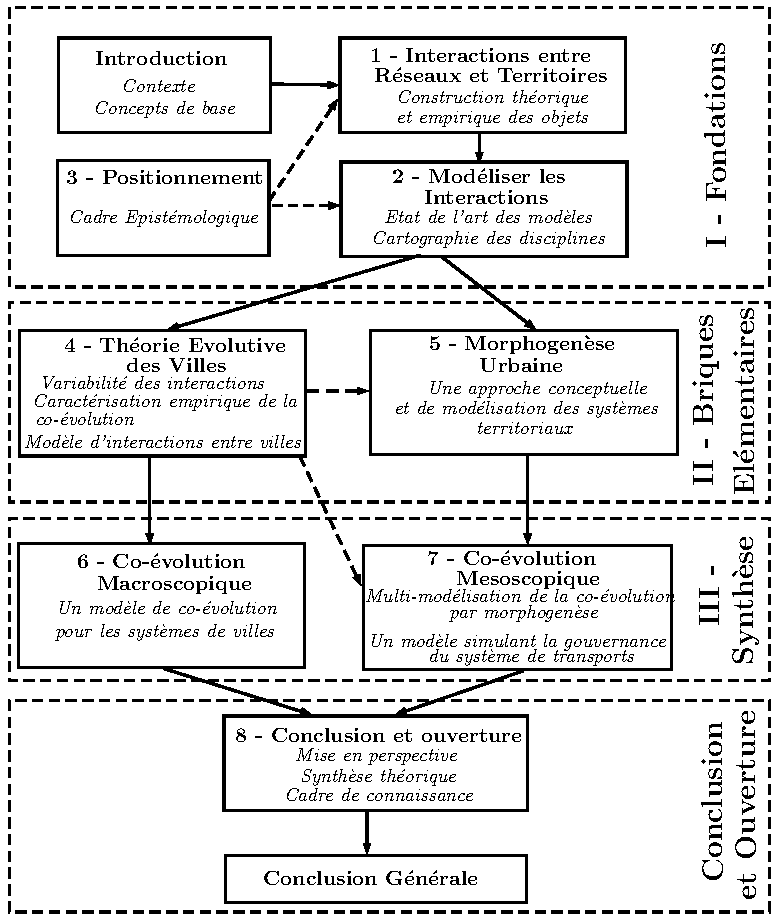
\includegraphics[width=\linewidth]{Figures/Theory/plan.pdf}
		
		\medskip
		
		\noun{Encadré : } \textit{Organisation générale du mémoire. Les flèches pleines donnent une dépendance directe (enchainement logique ou extensions), les flèches pointillées une dépendance indirecte (réutilisation de données ou de méthodes).}
		
	\end{mdframed}
\end{figure}
%%%%%%%%%%%


% \comment[AB]{intro = beau boulot !}

%\comment[FL]{Introduction \cn{关}
%\begin{itemize}
	%\item c'est seulement p11 que tu parles pour la premiere fois du sujet. Avant c'est de l'epistemo : pas une introduction a la these, mais une discussion - tres utile - sur les champs scientifiques. Garde cette discussion mais commence par une vraie introduction.[non, prefere garder cette strategie]
	%\item fin OK $\rightarrow$ et à positionner avant la partie epistemo.
%\end{itemize}
%}




%\paragraph{On linear reading}{Sur la lecture linéaire}

%%%%%%%
%% -- ON HOLD -- (depends on reflexive analysis - last appendix)


%\comment{expliquer notre position sur la difficulté d'une présentation linéaire, au delà de faire la synthèse. // bon bouquins y arrivent ? y réfléchir. la métaphore narrative intro/cl parties sera ce squelette linéaire. les deux approches sont compatibles.}


%\bpar{
%Research question and precise objects are deliberately fuzzy for now, as we postulate that the construction of a problematic can not be dissociated from the production of a corresponding theory. Reciprocally, it makes no sense to ask questions out of the blue, on objects that have been only partially or rapidly defined. Our preliminary question to enter the subject, that we can obtain from concrete cases such as our introducing anecdote or from preliminary literature review, is the following :
%}{
%Dans tous les cas, nous postulons que la construction d'une problématique ne peut être dissociée de la production d'une théorie correspondante. De manière réciproque, il n'y a aucun sens à poser des questions sorties de nulle part, sur des objets qui ont été seulement partiellement ou brièvement définis. Notre question préliminaire pour entrer dans le sujet, qu'on peut obtenir à partir de cas concrets comme l'anecdote introductive ou la revue de littérature préliminaire, est la suivante :
%}









\stars








%----------------------------------------------------------------------------------------

\ctparttext{This part set up foundations, constructing our research precise subject and questions from a thematic point of view, completed with a theoretical construction for framing at thematic and epistemological levels. We also provide methodological digressions, and a quantitative epistemological analysis completing the manual state of the art. \comment{(Arnaud) ça s'appelle lire}}

% Part I : methodology / theory / meta-theory
%\part{Thematic, Theoretical and Methodological Foundations} % First part of the thesis
%\part{Foundations : setting up the ground and roots}
\part{Foundations}


% -- Remark : the architectural metaphor is nice to introduce diverse parts --


%%%%%%%%%%%%%%%%%%%%%%%%%%%%%
% Chapter 1 : Thematic


% Chapter 




%\chapter{Interactions between Networks and Territories}{Interactions entre Réseaux et Territoires} % Chapter title
\chapter{Interactions entre Réseaux et Territoires}


\label{ch:thematic} % For referencing the chapter elsewhere, use \autoref{ch:name} 




%----------------------------------------------------------------------------------------

%\headercit{If you are embarrassed by the precedence of the chicken by the egg or of the egg by the chicken, it is because you are assuming that animals have always be the way they are}{Denis Diderot}{\cite{diderot1965entretien}}

%\headercit{Si la question de la priorit{\'e} de l'\oe{}uf sur la poule ou de la poule sur l'\oe{}uf vous embarrasse, c'est que vous supposez que les animaux ont {\'e}t{\'e} originairement ce qu'ils sont {\`a} pr{\'e}sent.
%}{Denis Diderot}{\cite{diderot1965entretien}}


\bigskip


\bpar{
This analogy is ideal to evoke the questions of causality and processes in territorial systems. When trying to tackle naively our preliminary question, some observers have qualified the identification of causalities in complex systems as ``chicken and egg'' problems : if one effect appears to cause another and reciprocally, how can one disentangle effective processes ? This vision is often present in reductionist approaches that do not postulate an intrinsic complexity in studied systems. The idea that Diderot suggests is the notion of \emph{co-evolution} that is a central phenomenon in evolutive dynamics of Complex Adaptive Systems as \noun{Holland} develops in~\cite{holland2012signals}. He links the notion of emergence (that is ignored in a reductionist vision), in particular the emergence of structures at an upper scales from the interactions between agents at a given scale, materialized generally by boundaries, that become crucial in the coevolution of agents at any scales : the emergence of one structure will be simultaneous with one other, each exploiting their interrelations and generated environments conditioned by their boundaries. We shall explore these ideas in the case of territorial systems in the following.
}{
Pour mieux visualiser les notions de causalités circulaires dans les systèmes complexes, et pourquoi celles-ci peuvent conduire à des paradoxes en apparence, l'image fournie par \noun{Diderot} dans~\cite{diderot1965entretien} est idéale : ``\textit{Si la question de la priorit{\'e} de l'\oe{}uf sur la poule ou de la poule sur l'\oe{}uf vous embarrasse, c'est que vous supposez que les animaux ont {\'e}t{\'e} originairement ce qu'ils sont {\`a} pr{\'e}sent}''. En voulant traiter naïvement des questions similaires induites par notre problématique introduite précédemment, certains ont qualifié les causalités au sein de systèmes complexes géographiques comme un problème ``de poule et {\oe}uf'' : si un effet semble causer l'autre et réciproquement, est-il possible et même pertinent de vouloir isoler les processus correspondants ? Cette question est bien connue des planificateurs des transports, comme le rappelle la notion des ``effets structurants'' qui fait débat depuis un certain temps au moins dans la communauté scientifique \comment[FL]{non cela va trop vite}. Une vision simplifiée, selon laquelle on peut attribuer des rôles systématiques à une composante particulière, est souvent présente dans les approches réductionnistes qui ne postulent pas une complexité intrinsèque au sein des systèmes étudiés.\comment[FL]{mots pas clairs ; a la place : amener co-evolution} L'idée suggérée par \noun{Diderot} est celle de \emph{co-evolution} qui est un phénomène central dans les dynamiques évolutionnaires des Systèmes Complexes Adaptatifs comme \noun{Holland} élabore dans~\cite{holland2012signals}. Il fait le lien entre l'émergence de structures à une échelle supérieure par les interactions entre agents à une échelle donnée, en général concrétisée par un systèmes de limites\comment[FL]{pas clair}, qui devient cruciale pour la co-évolution des agents à toutes les échelles : l'émergence d'une structure sera simultanée avec une autre, chacune exploitant leur interrelations et environnements générés conditionnés par le système de limites.\comment[FL]{rupture : le fil n'est pas clair} Nous explorerons ces idées pour le cas des systèmes territoriaux par la suite. Ceux-ci illustrent parfaitement ces problématiques, et sont typiques de systèmes dans lesquels cette complexité\comment[FL]{laquelle} est cruciale pour une appréhension raisonnable des mécanismes impliqués dans leurs dynamiques. Un certain nombre d'illustrations concrètes\comment[FL]{de quoi ?} seront d'abord données pour formuler nos questionnements dans des contextes géographiques donnés.\comment[FL]{phrase inutile}
}



\bpar{
This introductive chapter aims to set up the thematic scene, the geographical context in which further developments will root. It is not supposed to be understood as an exhaustive literature review nor the fundamental theoretical basement of our work (the first will be an object of chapter~\ref{ch:quantepistemo} whereas the second will be earlier tackled in chapter~\ref{ch:theory}), but more as narration aimed to introduce typical objects and views and construct naturally research questions.
}{
Ce chapitre introductif est destiné à poser le cadre thématique, les contextes géographiques sur lesquels les développements suivants se baseront.\comment[FL]{plus haut} Il n'est pas supposé être compris comme une revue de littérature exhaustive ni comme les fondations théoriques fondamentales de notre travail, le premier point étant l'objet du chapitre~\ref{ch:modelinginteractions} tandis que le second sera traité systématiquement dans le chapitre~\ref{ch:theory} lorsque le recul nécessaire aura été progressivement construit. Il doit plutôt être lu comme une construction narrative ayant pour but d'introduire nos objets et positions d'étude.\comment[FL]{cela sera dans l'intro generale} La notion de co-évolution est particulièrement pertinente\comment[FL]{oui : a remonter} pour comprendre les interactions entre territoires et réseaux. Dans une première section~\ref{sec:networkterritories}, nous préciserons l'approche prise de l'objet territoire, et dans quelle mesure celui-ci naturellement implique la considération des réseaux de transport pour la compréhension des dynamiques couplées. Ces considérations abstraites seront illustrées par des cas d'étude concrets dans la deuxième section~\ref{sec:casestudies}, choisis très différents pour comprendre les enjeux d'universalité sous-jacents. Enfin, dans la troisième section~\ref{sec:qualitative},des éléments d'observation de terrain effectués en Chine préciseront encore ces exemples aux échelles microscopique et mesoscopique. \comment[FL]{reprendre}
}



\stars


\textit{Ce chapitre est entièrement inédit.}\comment[FL]{ne pas dire cela}[(JR) permet d'avoir une unite avec les autres chapitres.]







%-------------------------------




























%%%%%%%%%%%%%%%%%%%%%%%%%%%%%


%%%%%%%%%%%%%%%%%%%%%%%%%%%%%
% Chapter 2 : Modeling the Interactions


%\chapter{Modeling Interactions between Networks and Territories}{Modéliser les Interactions entre Réseaux et Territoires} % Chapter title
\chapter{Modéliser les Interactions entre Réseaux et Territoires}


\label{ch:modelinginteractions}

%----------------------------------------------------------------------------------------




Si la littérature empirique et thématique, ainsi que les cas d'études développés précédemment\comment[FL]{NB: comme je commence par lire des 2 je ne les ai pas en tete}, semblent converger vers un consensus sur la complexité des relations entre réseaux et territoires\comment[FL]{mots qu'il conviendra d'avoir definis precedemment}, et\comment[FL]{faire deux phrases} dans certaines configurations et à certaines échelles de relations circulaires causales entre dynamiques territoriales et dynamiques des réseaux de transports\comment[FL]{pourquoi dans la premiere partie de la phrase il ny a pas transports et la oui?} que l'on se proposera de désigner par \emph{co-évolution}\comment[FL]{faire une tournure de phrase plus simple pour definir le not coevolution}, ceux-ci semblent diverger sur toute explication potentiellement simple\comment[FL]{mal dit} ou systématique, comme le rappelle par exemple les débats autour des effets structurants des infrastructures~\cite{offner1993effets}\comment[FL]{qu'il convient ici d'expliciter en 2.3 - $\phi$ : qui dit quoi dans ce debat ?}. Au contraire, les multiples situations géographiques poussent à privilégier des études ciblées très fortement dépendantes du contexte et du travail de terrain\comment[FL]{phrase un peu rapide tu donnes l'impression que tu tranches le debat}. Or l'explication géographique et la compréhension des processus est très vite limitée dans cette approche, et intervient un besoin d'un certain niveau d'abstraction et de généralisation\comment[FL]{or justement il convient d'expliciter ce debat theorie vs empirisme (ou autre)$\rightarrow$dans la phrase en pointilles tu parles d'un besoin d'abstraction, ce nest pas le terme scientifique}. C'est sur un tel point que la Théorie Evolutive des Villes se concentre particulièrement\comment[FL]{il faut absolument se departir d'un ton enthousiaste non scientifique. tu te proposes d'appliquer une theorie/un cadre analytique a une question - ca marche plus ou moins, cest tout, il ne doit pas y avoir d'a priori ou de preference de ton cote}, puisqu'elle arrive à combiner des schémas et modèles généraux aux particularités géographiques, et en tire même parti, tandis\comment[FL]{faire deux phrases} que certaines théories issues de la physique comme la Théorie du Scaling de \noun{West}~\cite{west2017scaling} peuvent être plus difficile à digérer pour les géographes\comment[FL]{tu pars deja dans de l'interpretation epistemo : il faut séparer les choses, d'abord de quoi s'agit-il ?} de par leur positionnement d'universalité qui est à l'opposé de leurs épistémologies habituelles. Dans tous les cas, le \emph{medium} qui permet de gagner en généralité sur les processus et structures des systèmes est toujours le \emph{modèle}\comment[FL]{l'italique ne joue pas le meme role pour les 2 mots cela prete a confusion} (voir \ref{sec:knowledgeframework} pour un développement des domaines de connaissance et du rôle du modèle). Comme le rappelle \noun{J.P. Marchand}~\cite{raimbault2017entretiens}, ``notre génération a compris qu'il y avait une co-évolution, la votre cherche à la comprendre''\comment[FL]{TB citation a mettre en italique}, ce qui appuie le pouvoir de compréhension apporté par la modélisation et la simulation qui pourraient être aujourd'hui à leur balbutiements\comment[FL]{ok avec le sens de cette phrase mais le conditionnel sonne mou. si tu as des arguments avance les, sinon dis clairement auelle est ta position}. Sans développer les innombrables fonctions que peut avoir un modèle, nous nous baserons sur l'adage\comment[FL]{terme non scientifique} de \noun{Banos} qui soutient que ``modéliser c'est apprendre'', et suivant notre positionnement dans une science des systèmes complexes suggéré en introduction, nous ferons ainsi de la \emph{modélisation des interactions entre réseaux et territoires} notre principal sujet d'étude, outil, objet (même si dans une lecture rigoureuse de~\ref{sec:knowledgeframework} ce positionnement n'a pas de sens puisque notre démarche contenait déjà des modèles à partir du moment où elle était scientifique\comment[FL]{tu ne peux pas parler d'une lecture rigoureuse de tes propres propos ! supprime la ()}). Ce chapitre peut être vu comme un ``état de l'art'' des démarches de modélisation des interactions entre réseaux et territoires. Il vise en particulier à être aussi objectif et exhaustif que possible\comment[FL]{mal amene, cest souvent le but non ?} : pour cela, nous mobiliserons des analyses en épistémologie quantitative. Dans une première section~\ref{sec:modelingsa}, nous passons en revue de manière interdisciplinaire les modèles pouvant être concernés, même de loin, sans a priori d'échelle temporelle ou spatiale, d'ontologies, de structure, ou de contexte d'application. Les modèles de changement d'usage du sol très appliqués en planification sont tout autant concernés que des modèles totalement abstraits issus de la biologie ou de la physique, que des approches intégrées en géographie ou spécifiques en économie\comment[FL]{pas utile ici tu detailleras en 2.1 : ici affirmer les objectifs (quelle information en retirer) et les moyens (par ez meme automatique tu as bien un (des) points d'entrees $\rightarrow$ lesquels et pourquoi?}. Cet aperçu suggère des structures de connaissances assez indépendantes et des disciplines ne communiquant que rarement\comment[FL]{B}. Nous procédons à une revue systématique algorithmique\comment[FL]{est-ce une facon standard de nommer cela ?}[(JR) l'exploration iterative de la facon dont elle est faite n'a jamais ete faite a ma connaissance, j'introduis donc une ``nouvelle'' façon de faire.] dans~\ref{sec:quantepistemo} pour reconstruire leur paysage scientifique, dont les résultats tendent à confirmer ce cloisonnement\comment[FL]{c'est interessant bien sur mais il faut dire pourquoi tu vises cela. a mon avis il vaut mieux commencer par des exemples de manieres dont la litterature sci. prend en compte ces interactions, dans differentes disciplines, avant d'atteindre l'epistemologie quantitative.}. L'étude est complétée par une analyse d'hyperréseau, combinant réseau de citation et réseau sémantique issu d'analyse textuelle, qui permet de mieux cerner les relations entre disciplines, leur champs lexicaux et leur motifs d'interdisciplinarité. Cette étude permet la constitution du corpus utilisé pour la modélographie et la meta-analayse\comment[FL]{mots qui nont pas encore ete introduits} effectuée en dernière section~\ref{sec:modelography}, qui dissèque la nature d'un certain nombre de modèles et la relie au contexte disciplinaire, ce qui pose les bases et le cadre précis des efforts de modélisation qui seront développés par la suite.






\stars


\textit{Ce chapitre est inédit pour sa première section ; reprend dans sa deuxième section le texte traduit de~\cite{raimbault2015models}, puis pour sa deuxième partie la méthodologie de \cite{raimbault2016indirect}, les outils de \cite{bergeaud2017classifying} et des passages de~\cite{}; et est enfin inédit pour sa dernière partie.}

\comment[FL]{mettre bout a bout tous ces passages (non classiques, mais que je trouve beinvenus, en toute fin d'intro generale)}[à rediscuter, je trouve ca plus adapté pour chaque chapitre dans le cadre d'une ``these a papiers'' (meme si c'est est pas une officiellement).]







%%%%%%%%%%%%%%%%%%%%%%%%%%%%%



%%%%%%%%%%%%%%%%%%%%%%%%%%%%%
% Chapter 3 : Positioning



% Chapter 

%\chapter{Positioning}{Positionnements} % Chapter title
\chapter{Positionnements}


\label{ch:positioning} % For referencing the chapter elsewhere, use \autoref{ch:name} 

%----------------------------------------------------------------------------------------

%\headercit{}{}{}

\bigskip


Toute activité de recherche serait, selon certains observateurs, nécessairement politisée, de par pour commencer le choix de ses objets. Ainsi, \noun{Ripoll} alerte contre l'illusion d'une recherche objective et les dangers de la technocratie~\cite{ripoll2017jig}. Nous ne rentrerons pas dans ces débats bien trop vastes pour être traités même en un chapitre, puisqu'il rejoignent des thèmes de sciences politiques, d'éthique, de philosophie, liés par exemple à la gouvernance scientifique, à l'insertion de la science dans la société, à la responsabilité scientifique. Il est clair que même des sujets a priori intrinsèquement objectifs, comme la physique des particules et des hautes énergies, ont des implications regardant d'une part les choix de leur financements et les externalités associées (par exemple, l'existence du CERN a largement contribué au développement du calcul distribué), mais d'autre part aussi les applications potentielles des découvertes qui peuvent avoir des répercussions sociales gigantesque. En biologie, l'éthique est au coeur des principes fondateurs des disciplines, comme en témoigne les débats soulevés par l'émergence de la biologie synthétique~\cite{}. % TODO cit. bio synth
\todo{add a development sur socially responsible integartive sciences etc.}
 En sciences humaines, comme les recherches interagissent avec les objets étudiés (en quelque sorte l'idée des \emph{interactive kind} de \noun{Hacking}~\cite{hacking1999social}), les implications politiques et sociales de la recherche sont bien évidemment indiscutables. Là où il y aurait matière à discussion, et nous y reviendrons en ouverture~\ref{} car il s'agira d'une des questions ouvertes posées par notre recherche et sa démarche dans leur ensemble, serait sur la compatibilité des méthodes systématiques et \emph{evidence-based} avec les sciences sociales, autrement dit dans quelle mesure peut-on s'extraire de certains dogmatismes encore plus marqués lors de l'usage de théorie politiques\footnote{\noun{Monod} montre par exemple les désastres liés aux ``niaiseries épistémologiques'' découlant de l'application littérale de la dialectique matérialiste marxiste à l'épistémologie du vivant.}. Nous resterons ici à un niveau épistémologique, c'est à dire à des réflexions sur la nature et le contenu des connaissances scientifiques au sens large, c'est à dire co-construites et validées au sein d'une communauté imposant certains critères de scientificité, bien sûr évolutifs puisque nous nous positionnerons pour la systématisation de certains. Mais donc, même en restant à ce niveau, des prises de positions sont nécessaires, celles-ci pouvant être épistémologiques, méthodologiques, thématiques. Ces dernières ont déjà été ébauchée dans les deux chapitres précédents par les choix des objets d'étude, des problématiques, et seront renforcées à mesure de la progression pour finalement être synthétisées en Chapitre~\ref{ch:theory}. Nous proposons ici un exercice relativement original mais que nous jugeons nécessaire pour une lecture plus fluide de la suite, qui consiste en le développement précis de certains positionnements qui ont une influence particulière dans notre démarche de recherche. Par exemple, le travail en données quasi-intégralement ouverte et en architecture modulaire résulte de notre exigence de reproductibilité. L'utilisation des modèles et la manière de les explorer de notre vision du calcul intensif. Dans une première section (\ref{sec:reproducibility}), nous développons des exemples pour illustrer le besoin et la difficulté de reproductibilité, ainsi que les liens avec des nouveaux outils pouvant la favoriser mais aussi la mettre en danger. Dans une deuxième section (\ref{sec:computation}), nous argumentons sous forme d'essai pour un usage raisonné des données massives et du calcul intensif, et illustrons notre positionnement par rapport à l'exploration des modèles par une étude de cas méthodologique pour l'exploration de la sensibilité des modèles aux conditions initiales. Enfin, la dernière section (\ref{sec:epistemology}) explicite modestement des positions épistémologiques, notamment concernant le courant dans lequel nous nous plaçons, la complexité des objets en sciences sociales, et la nature de la complexité de manière générale.




\stars


\textit{Ce chapitre est composé de divers travaux. La première section est inédite. La deuxième section rend compte pour sa première partie du contenu théorique de \cite{raimbault2016cautious}, et pour sa deuxième partie des idées et de passages adaptés de \cite{} % TODO cit. geocomputation
et de \cite{}. % TODO cit. Space Matters paper.
 La troisième section reprend dans sa première partie les bases épistémologiques de \cite{raimbault:halshs-01505084} approfondies par \cite{} % cit knowledge framework
, est inédite pour sa deuxième partie et rend compte de \cite{} % cit. Geodivercity
 pour sa dernière partie.
}







%%%%%%%%%%%%%%%%%%%%%%%%%%%%%



%%%%%%%%%%%%%%%%%%%%%%%%%%%%%
% Chapter : Methodo



% Chapter 

%\chapter{Methodological Developments}{Développements Méthodologiques} % Chapter title
\chapter{Développements méthodologiques}


\markboth{\thechapter\space Développements Méthodologiques}{\thechapter\space Développements Méthodologiques}


\label{app:methodology} % For referencing the chapter elsewhere, use \autoref{ch:name} 

%----------------------------------------------------------------------------------------

%\headercit{We are now building a rigorous Science of Cities, contrarily to what was done before.}{Marc Barth{\'e}l{\'e}my}{EMCSSS Fall 2014, Network Course Introduction}

%\headercit{C'est hardcore tes calculs.}{Anonyme}{}

%This chapter gathers various methodological and technical developments, that have the common points to be not essential to the core of the thesis and difficult to digest.



Cette annexe rassemble différents développements méthodologiques qui sont utilisés indirectement, ou permettre de creuser des questions liées mais non centrales à notre fil principal.

Les trois premières sections traitent des questions se posant particulièrement lors de l'étude des systèmes urbains ou territoriaux.
\begin{enumerate}
	\item Un lien formel entre différents modèles stochastiques de croissance urbaine permet de poser un cadre général pour ce genre d'approche, et d'illustrer le lien implicite entre notre approche mesoscopique et notre approche macroscopique.
	\item La sensibilité des lois d'échelles à la définition de la ville est étudiée analytiquement pour un modèle simple de système urbain. Cette perspective renforce la méthodologie d'analyse de sensibilité des modèles à la configuration spatiale introduite en~\ref{sec:computation}.
	\item Le contexte bibliographique et formel de la notion de données synthétiques permet également de situer celle-ci.
\end{enumerate}

Nous développons ensuite des cadres méthodologiques généraux liés à l'étude des systèmes.

\begin{enumerate}\setcounter{enumi}{4}
	\item Dans le cadre de systèmes incluant des optimisation multi-attributs, une méthode d'analyse de sensibilité à la structure des données, est introduite. Elle n'est pas directement appliquée dans notre travail mais suggère des pistes pour l'application des modèles mesoscopiques de morphogenèse, puisque ceux-ci se basent sur une telle optimisation par les agents.
	\item Un cadre général pour la modélisation des systèmes complexes socio-techniques, pose les premières bases d'une part d'une formalisation du \emph{perspectivisme appliqué} mais également de la formalisation du cadre de connaissances suggérée en~\ref{sec:knowledgeframework}.
\end{enumerate}

Enfin, le dernier développement concerne les méthodes d'épistémologie quantitative.

\begin{enumerate}\setcounter{enumi}{4}
	\item Les détails techniques de la méthode utilisée en~\ref{sec:quantepistemo} sont développés dans le cadre d'application au corpus de la revue \emph{Cybergeo}. Les considérations sont fondamentalement méthodologiques, et doivent être également mises en perspective avec l'article thématique companion que nous adaptons en~\ref{app:sec:cybergeonetworks}.
\end{enumerate}


%\stars

%Such a shocking phrase \comment{(Florent) je crois que si tu t'appuies explicitement sur la mise en exergue alors ce n'est plus une mise en exergue} was pronounced during the introduction of a \emph{Network} course for students of Complex System Science. Besides the fact that the spirit of CSS \comment{(Florent) pas mettre trop d'acronymes que tu ne réutiliseras pas} is precisely the opposite, {\ie} the construction of integrative disciplines (vertical integration that is necessarily founded on the existing body of knowledge of concerned fields) that answer transversal questions (horizontal integration that imply interdisciplinarity) - see {\eg} the roadmap for CS~\cite{2009arXiv0907.2221B}, it reveals how methodological considerations shape the perceptions of disciplines. From a background in Physics, \comment{(Florent) soit on connaitre ton background ?} ``rigorous'' implies the use of tools and methods judged more rigorous (analytical derivations, large datasets statistics, etc.).\comment{(Florent) je ne suis pas sur que cela soit ca la rigueur physicienne. ce serait plutôt un raisonnement sans trou du début à la fin sur des objets clairement définis ; en sciences sociales il y a fréquemment des trous} But what is rigorous for someone will not be for an other discipline\footnote{a funny but sad anecdote told by a friend comes to mind : defending his PhD in statistics, he was told at the end by economists how they were impressed by the mathematical rigor of his work, whereas a mathematician judged that ``he could have done everything on the back of an enveloppe''.\comment{(Florent) ce n'est pas lié à la rigueur}}, depending on the purpose of each piece of research (perspectivism~\cite{giere2010scientific} poses the \emph{model}, that includes methods, as the articulating core of research entreprises). Thus the full role of methodology aside and not beside theory and experiments. We go in this chapter into various methodological developments which may be precisely used later or contribute to the global background.


%\bpar{
%We then derive technical results on models of urban growth and on the sensitivity of scaling laws, that are both recurrent themes in the modeling of complex urban systems. We then introduce a method in the context of systematic model exploration and model behavior. We finally work on a link between static and dynamic correlations in a geographical system. This chapter is rather heteroclite as sections may correspond to a particular technical need at a point in the thesis, to global methodological directions, or global research directions.
%}{

%}




%----------------------------------------------------------------------------------------

\newpage

\section{An unified framework for stochastic models of urban growth}{Modèles stochastiques de croissance urbaine}


\label{app:sec:stochurbgrowth}


\bpar{
Urban growth modeling fall in the case of tentatives to find self-consistent rules reproducing dynamics of an urban system, and thus in our logic of system morphogenesis. We examine here methodological issues linked to different frameworks of urban growth.
}{
Les différents modèles stochastiques de croissance urbaine que nous avons développé suivent la même logique de règles autonomes pour reproduire les dynamiques des systèmes urbains. Nous proposons ici d'un point de vue méthodologique de mettre en valeur les liens entre les différents cadres, afin d'en formuler un cadre unifié.
}


%%%%%%%%%%%%%%%%%%%%
\subsection{Introduction}{Introduction}
%%%%%%%%%%%%%%%%%%%%


\bpar{
Various stochastic models aiming to reproduce population patterns on large temporal and spatial scales (city systems) have been discussed across various fields of the literature, from economics to geography, including models proposed by physicists. We propose here a general framework that allows to include different famous models (in particular Gibrat, Simon and Preferential Attachment model) within an unified vision. %It brings first an insight into epistemological debates on the relevance of models. 
Furthermore, bridges between models lead to the possible transfer of analytical results to some models that are not directly tractable.
}{
Divers modèles stochastiques de croissance urbaine visant à reproduire des trajectoires de population, ou des faits stylisés sur celles-ci, souvent sur de longues échelles de temps et de grandes étendues spatiales (systèmes de villes) ont été proposé par la littérature dans des champs variés, de l'économie ou la physique à la géographie (voir par exemple~\ref{sec:interactiongibrat} et \ref{sec:densitygeneration} pour des revues à différentes échelles). Nous proposons ici une approche générale permettant de faire le liens entre plusieurs modèles existant, plus particulièrement les modèles de Gibrat, de Simon et d'attachement préférentiel.
}


\bpar{
Seminal models of urban growth are Simon~\cite{simon1955class} (later generalized as e.g. \cite{haran1973modified}) and Gibrat models. Many examples of variants and extensions can be given across disciplines. \cite{benguigui2007dynamic} give an equation-based dynamical model, whereas \cite{gabaix1999zipf} shows that the Gibrat model produces Zipf's law in a stationary state. \cite{Gabaix20042341} reviews urban growth approaches in economics. A model adapted from evolutive urban theory is described in~\cite{favaro2011gibrat} and extends the Gibrat model by adding propagation of innovation between cities. The question of empirical scales at which it is consistent to study urban growth was also tackled in the particular case of France~\cite{bretagnolle2002time}, which shows that long time scales (more than a few decade) are appropriate to study dynamics of urban systems at a small spatial scale. 
%We stay to a certain level of tractability to include models as essence of our approach is links between models but do not make ontologic assumptions \comment[JR]{sens ?}.
}{
Des modèles fondamentaux de croissance urbaine sont les modèles de Gibrat (voir~\ref{sec:interactiongibrat}) et le modèle de Simon~\cite{simon1955class} (qui a plus récemment été généralisé, voir par exemple~\cite{haran1973modified}). Diverses extensions on été données selon les disciplines. \cite{benguigui2007dynamic} donne un modèle de système dynamique, tandis que \cite{gabaix1999zipf} montre que le modèle de Gibrat produit la loi de Zipf pour la distribution de la taille des villes dans l'état stationnaire. Les approches en économie sont revues par \cite{Gabaix20042341}. Un modèle inspiré par la Théorie Evolutive des Villes est décrit dans~\cite{favaro2011gibrat} et étend le modèle de Gibrat par l'addition de la propagation de l'innovation entre les villes. La question des échelles empiriques auxquelles ce type d'approche est pertinent a été traité dans le cas particulier de la France par~\cite{bretagnolle2002time}, qui montre que de longues échelles de temps (supérieures à quelques décades) sont appropriées pour étudier la dynamique des systèmes urbains à une petite échelle spatiale.
}



%%%%%%%%%%%%%%%%%%%%
\subsection{Framework}{Cadre de Travail}
%%%%%%%%%%%%%%%%%%%%


%\paragraph{Presentation}

\bpar{
What we propose as a framework can be understood as a meta-model, i.e. a modular general modeling process within each model can be understood as a limit case or as a specific case of another model. More simply it should be a diagram of formal relations between models.\comment{(Florent) à ce stade on ne sait pas si tu vas faire 1 ou N modèles, c'est un choix qu'il te faut défendre avant d'en arriver là}
The ontological aspect is also tackled by embedding the diagram into an ontological state space (which discretization corresponds to the ``bricks'' of the incremental construction of~\cite{cottineau2015incremental}). It constructs a sort of model classification or modelography. \comment{(Florent) PAS UTILE ICI JE PENSE}
}{
Le cadre que nous introduisons peut se comprendre comme un meta-modèle, au sens où chaque modèle peut être compris comme extension ou cas limite d'un autre modèle. 
}


%We are still at the stage of different derivations of links between models that are presented hereafter.

%\subsubsection{Models Included}

%The following models are included in our framework. The list is arbitrary but aims to offer a broad view of disciplines concerned

%\subsubsection{Thematic Classification}


%\subsubsection{Framework Formulation}
%Diagram linking various models ; first embedded into time/population plane, cases Discrete/Continous. Other aspects more sparse (ex. spatialization) ; how represent it ?

%   \comment{(Florent) on a déjà discuté de cette eq Gibrat/att pref mais tu ne peux pas faire l'économie d'expliquer pourquoi tu t'es posé la question, i.e. à quoi cela va te servir ensuite} -> justifier l'interet de ce lien


%%%%%%%%%%%%%%%%%%%%
%\subsection{Models formulation}



%%%%%%%%%%%%%%%%%%%%
\subsection{Derivations}{Dérivations}

\subsubsection{Generalization of Preferential Attachment}{Généralisation de l'Attachement Préférentiel}

\bpar{
\cite{yamasaki2006preferential} give a generalization of the classical Preferential Attachment Network Growth model, as a birth and death model with evolving entities. More precisely, network units gain and lose population (equivalent to links connexions) at fixed probabilities, and new unit can be created at a fixed rate.
}{
\cite{yamasaki2006preferential} donne une généralisation du modèle classique d'attachement préférentiel pour la croissance des réseaux, comme un modèle de vie et mort avec des entités évolutives. Plus précisément, les noeuds du réseau gagnent et perdent des unités de population à des probabilités fixes, et de nouveaux noeuds peuvent être ajoutés à un taux également fixe.
}

\subsubsection{Link between Gibrat and Preferential Attachment Models}{Lien entre Gibrat et Attachement Préférentiel}


\bpar{
Let consider a strictly positive growth Gibrat model given by $P_i(t)=R_i(t)\cdot P_{i}(t-1)$ with $R_i(t)>1$, $\mu_i(t)=\Eb{R_i(t)}$ and $\sigma_i(t)=\Eb{R_i(t)^2}$. On the other hand, we take a simple preferential attachment, with fixed attachment probability $\lambda \in [0,1]$ and new arrivants number $m>0$. We derive that Gibrat model can be statistically equivalent to a limit of the preferential attachment model, assuming that the moment-generating function of $R_i(t)$ exists. Classical distributions that could be used in that case, e.g. log-normal distribution, are entirely defined by two first moments, making this assumption reasonable.
}{
Considérons un modèle de croissance strictement positive de Gibrat donnée par $P_i(t)=R_i(t)\cdot P_{i}(t-1)$ avec $R_i(t)>1$, $\mu_i(t)=\Eb{P_i(t)}$, $\lambda_i(t)=\Eb{R_i(t)}$ et $\sigma_i(t)=\Eb{R_i(t)^2}$. Les $P_i$ sont les populations des villes tandis que $R_i$ sont des taux de croissance aléatoires. D'autre part, soit un modèle simple d'attachement préférentiel, avec une probabilité d'attachement $\lambda \in [0,1]$ et un nombre de nouveau arrivants $m>0$, ce qui revient en espérance à $\mu_i(t+1) - \mu_i(t) = m\cdot \lambda$. Il est possible de dériver que le Gibrat est statistiquement équivalent à une limite de l'attachement préférentiel, sous l'hypothèse que toutes les fonctions génératrices des moments de $R_i(t)$ existent. Les distributions classiques qui peuvent être utilisées dans ce cas, e.g. une distribution normale ou log-normale, sont entièrement déterminées par leur deux premiers moments, ce qui rend cette hypothèse raisonnable.
}

% \comment{(Florent) est-ce standard d'introduire de la stochasticité dans Gibrat : Pt+1=RPt}[c'est la formulation standard a priori]

\bpar{
\begin{lemma}
The limit of a Preferential Attachment model when $\lambda \ll 1$ is a linear-growth Gibrat model, with limit parameters $\mu_i(t)=1+\frac{\lambda}{m\cdot (t-1)}$.
\end{lemma}
}{
\begin{lemma}
	La limite d'un modèle d'attachement préférentiel quand $\lambda \ll 1$ est un modèle de croissance de Gibrat linéaire, avec le paramètres limites $\lambda_i(t)=1+\frac{\lambda}{m\cdot (t-1)}$.
\end{lemma}
}




\begin{proof}

\bpar{
Starting with first moment, we denote $\bar{P}_i(t)=\Eb{P_i(t)}$. Independence of Gibrat growth rate yields directly $\bar{P}_i(t)=\Eb{R_i(t)}\cdot \bar{P}_i(t-1)$. Starting for the preferential attachment model, we have $\bar{P}_i(t) = \Eb{P_i(t)} = \sum_{k=0}^{+\infty}{k\Pb{P_i(t)=k}}$. But
}{
S'intéressant au premier moment, nous notons $\bar{P}_i(t)=\mu_i(t)=\Eb{P_i(t)}$. L'indépendance entre les taux de croissance de Gibrat donne directement $\bar{P}_i(t)=\Eb{R_i(t)}\cdot \bar{P}_i(t-1)$. En partant du modèle d'attachement préférentiel, nous avons $\bar{P}_i(t) = \Eb{P_i(t)} = \sum_{k=0}^{+\infty}{k\Pb{P_i(t)=k}}$. Mais par ailleurs,
}
\[
\{P_i(t)=k\}=\bigcup_{\delta=0}^{\infty}{\left(\{P_i(t-1)=k-\delta\}\cap \{P_i\leftarrow P_i + 1\}^{\delta}\right)}
\]
\bpar{
where the second event corresponds to city $i$ being increased $\delta$ times between $t-1$ and $t$ (note that events are empty for $\delta \geq k$). Thus, being careful on the conditional nature of preferential attachment formulation, stating that $\Pb{\{P_i\leftarrow P_i + 1\} | P_i(t-1)=p} = \lambda\cdot\frac{p}{P(t-1)}$ (total population $P(t)$ assumed deterministic), we obtain
}{
où le second évènement correspond à la ville $i$ étant augmentée $\delta$ fois entre $t-1$ et $t$ (avec la convention que les évènement sont vides pour $\delta \geq k$). Ainsi, en prenant en compte la formulation conditionnelle de l'attachement préférentiel, qui postule que $\Pb{\{P_i\leftarrow P_i + 1\} | P_i(t-1)=p} = \lambda\cdot\frac{p}{P(t-1)}$ (la population totale $P(t)$ étant déterministe), nous obtenons
}
\begin{equation*}
\begin{split}
\Pb{\{P_i\leftarrow P_i + 1\}} & = \sum_{p}{\Pb{\{P_i\leftarrow P_i + 1\} | P_i(t-1)=p}\cdot \Pb{P_i(t-1)=p}}\\
&=\sum_{p}{\lambda\cdot\frac{p}{P(t-1)}\Pb{P_i(t-1)=p}}=\lambda\cdot\frac{\bar{P}_i(t-1)}{P(t-1)}\\
\end{split}
\end{equation*}

\bpar{
\noindent It gives therefore, knowing that $P(t-1)=P_0 + m\cdot (t-1)$ and denoting $q=\lambda\cdot\frac{\bar{P}_i(t-1)}{P_0 + m\cdot (t-1)}$
}{
\noindent Ce qui donne, sachant que $P(t-1)=P_0 + m\cdot (t-1)$ et en notant $q=\lambda\cdot\frac{\bar{P}_i(t-1)}{P_0 + m\cdot (t-1)}$
}


\[
\begin{split}
\bar{P}_i(t) & =\sum_{k=0}^{\infty}{\sum_{\delta=0}^{\infty}{k\cdot \left(\lambda\cdot\frac{\bar{P}_i(t-1)}{P_0 + m\cdot (t-1)}\right)^{\delta}\cdot \Pb{P_i(t-1)=k-\delta}}}\\
& = \sum_{\delta^{\prime}=0}^{\infty}{\sum_{k^{\prime}=0}^{\infty}{\left(k^\prime + \delta^{\prime}\right)\cdot q^{\delta^{\prime}} \cdot \Pb{P_i(t-1)=k^\prime}}}\\
& = \sum_{\delta^{\prime}=0}^{\infty}{q^{\delta^{\prime}}\cdot \left(\delta^{\prime} + \bar{P}_i(t-1)\right)} = \frac{q}{(1-q)^2} + \frac{\bar{P}_i(t-1)}{(1-q)}\\
& = \frac{\bar{P}_i(t-1)}{1-q}\left[1 + \frac{1}{\bar{P}_i(t-1)}\frac{q}{(1-q)}\right]
\end{split}
\]

%& = \bar{P}_i(t-1)\cdot \frac{1}{1-\lambda\cdot\frac{\bar{P}_i(t-1)}{P_0 + m\cdot (t-1)}} \left[1 + \frac{\lambda}{P_0 + m\cdot (t-1)}\cdot \frac{1}{1-\lambda\cdot\frac{\bar{P}_i(t-1)}{P_0 + m\cdot (t-1)}} \right]


\bpar{
As it is not expected to have $\bar{P}_i(t)\ll P(t)$ (fat tail distributions), a limit can be taken only through $\lambda$. Taking $\lambda \ll 1$ yields, as $0 < \bar{P}_i(t)/P(t) < 1$, that $q=\lambda\cdot\frac{\bar{P}_i(t-1)}{P_0 + m\cdot (t-1)} \ll 1$ and thus we can expand in first order of $q$, what gives $\bar{P}_i(t)=\bar{P}_i(t-1)\cdot \left[1 + \left(1+\frac{1}{\bar{P}_i(t-1)}\right)q + o(q))\right]$
}{
On s'attend à ce que pour la majorité des villes, $\bar{P}_i(t)\ll P(t)$ (distributions fortement dissymétriques), la limite peut être prise pour $\lambda$ uniquement. En prenant $\lambda \ll 1$, comme $0 < \bar{P}_i(t)/P(t) < 1$, nous obtenons $q=\lambda\cdot\frac{\bar{P}_i(t-1)}{P_0 + m\cdot (t-1)} \ll 1$, qui peut être développée au premier ordre en $q$. Cela donne finalement
}

\[
\bar{P}_i(t)=\bar{P}_i(t-1)\cdot \left[1 + \left(1+\frac{1}{\bar{P}_i(t-1)}\right)q + o(q))\right]
\]

et donc

\[
\bar{P}_i(t) \simeq \left[1 + \frac{\lambda}{P_0 + m\cdot (t-1)}\right]\cdot \bar{P}_i(t-1)
\]

\bpar{
It means that this limit is equivalent in expectancy to a Gibrat model with $\mu_i(t) = \mu(t)=1 + \frac{\lambda}{P_0 + m\cdot (t-1)}$.
}{
Cela signifie que cette limite est équivalente en espérance à un modèle de Gibrat avec $\mu_i(t) = \mu(t)=1 + \frac{\lambda}{P_0 + m\cdot (t-1)}$.
}

\bpar{
For the second moment, we can do an analog computation. We have still \[\Eb{P_i(t)^2} = \Eb{R_i(t)^2}\cdot \Eb{P_i(t-1)^2}\]
and
\[\Eb{P_i(t)^2}=\sum_{k=0}^{+\infty}{k^2 \Pb{P_i(t)=k}}\] 
}{
Pour le second moment, on peut faire un calcul similaire. On a toujours  \[\Eb{P_i(t)^2} = \Eb{R_i(t)^2}\cdot \Eb{P_i(t-1)^2}\]
et
\[\Eb{P_i(t)^2}=\sum_{k=0}^{+\infty}{k^2 \Pb{P_i(t)=k}}\] 
}

\bpar{
We obtain the same way 
}{
On obtient ainsi de la même façon
}

\[
\begin{split}
\Eb{P_i(t)^2} & = \sum_{\delta^{\prime}=0}^{\infty}{\sum_{k^{\prime}=0}^{\infty}{\left(k^\prime + \delta^{\prime}\right)^2\cdot q^{\delta^{\prime}} \cdot \Pb{P_i(t-1)=k^\prime}}}\\ 
& = \sum_{\delta^{\prime}=0}^{\infty}{q^{\delta^{\prime}}\cdot \left(\Eb{P_i(t-1)^2}+2\delta^{\prime}\bar{P}_i(t-1) + {\delta^{\prime}}^2\right)}\\
& = \frac{\Eb{P_i(t-1)^2}}{1-q} + \frac{2 q \bar{P}_i(t-1)}{(1-q)^2} + \frac{q(q+1)}{(1-q)^3}\\
& = \frac{\Eb{P_i(t-1)^2}}{1-q}\left[1 + \frac{q}{\Eb{P_i(t-1)^2}}\left(\frac{2\bar{P}_i(t-1)}{1-q} + \frac{(1+q)}{(1-q)^2}\right)\right]
\end{split}
\]


\bpar{
We have therefore an equivalence between the Gibrat model as a continuous formulation of a Preferential Attachment (or Simon model) in the limit given before. \qed
}{
On a ainsi équivalence entre le modèle de Gibrat et une formulation continue de l'Attachement préférentiel (ou du modèle de Simon) dans la limite donnée ci-dessus. \qed
}

\end{proof}






\subsubsection{Link between Simon and Preferential Attachment}{Lien entre Simon et Attachement Préférentiel}
%\label{subsubsec:gibrat-simon}

\bpar{
A rewriting of Simon model yields a particular case of the generalized preferential attachment, in particular by vanishing death probability.
}{
Une reformulation du modèle de Simon le présente comme un cas particulier de l'attachement préférentiel généralisé, en particulier avec la probabilité de mort nulle.
}

\subsubsection{Link between Favaro-Pumain and Gibrat}{Lien entre Favaro-Pumain et Gibrat}

\bpar{
\cite{favaro2011gibrat} generalizes Gibrat models with innovation propagation dynamics. Theoretically, a process-based model equivalent to the Favaro-Pumain should then fill the missing case in model classification at the corresponding discretization. Simpop models do not fill that case as they stay at the scale of city systems, as for Marius models~\cite{cottineau2014evolution}. These must also have their counterparts in discrete microscopic formulation.
}{
\cite{favaro2011gibrat} généralise le modèle de Gibrat avec les dynamiques de propagation de l'innovation. En théorie, un équivalent microscopique devrait pouvoir être formulé si on considère l'ensemble des modèles dans une typologie par ontologie et par paradigme. %Les modèles Simpop restent dans la catégorie
Les modèles Marius~\cite{cottineau2014evolution} correspondent à un paradigme de Gibrat, et devraient aussi avoir leur contrepartie en termes de formulation microscopique.
}

%\comment{(Florent) la encore tu parles de modèles que tu ne décris pas par ailleurs ; or Personnes connaissant FavaraoPumain $\cap$ Personnes connaissant Gibrat $\cap$ \ldots = quelques personnes sur terre! }[voir revues main text]

%\subsubsection{Link between Bettencourt-West and Pumain}{Lien entre Bettencourt-West et Pumain}

%We are considering to study Bettencourt-West model for urban scaling laws \cite{bettencourt2008large} as entering the stochastic urban growth framework as stationary component of a random growth model, but investigation are still ongoing.

%\comment{(Florent) on ne sait toujours pas dans quelle perspective tu fais cela}


%\subsubsection{Other Models}{Autres modèles}

%\cite{gabaix1999zipf} develops an economic model giving a Simon equivalent formulation. They in particular find out that in upper tail, proportional growth process occurs. We find the same result as a consequence of the derivation of the link between Gibrat and Preferential attachment models.

%\comment{(Florent) je pense que tu as intérêt soit à présenter moins de modèles, mais plus en détails, soit à partir d'angles d'attaque précis et faire des typologies de modèles}



\stars





%----------------------------------------------------------------------------------------

\newpage



\section{Sensitivity of Urban Scaling Laws to Spatial Extent}{Sensibilité des lois d'échelle urbaines}

\label{app:sec:scaling}


\bpar{
At the center of evolutive urban theory are hierarchy and associated scaling laws. We develop here a brief methodological investigation on the sensitivity of scaling laws to city definition.
}{
Au centre de la théorie évolutive des villes se trouvent la hiérarchie et les lois d'échelle associées. Nous proposons ici un bref développement méthodologique sur la sensibilité des lois d'échelle à la définition de la ville. %\comment{(Florent) présenté comme cela ce n'est pas évident de comprendre le rapport avec ta thèse}
}


%%%%%%%%%%%%%%%%%%%%
%\subsection{Introduction}



\bpar{
Scaling laws have been shown to be universal of urban systems at many scales and for many indicators. Recent studies question however the consistence of scaling exponents determination, as their value can vary significantly depending on thresholds used to define urban entities on which quantities are integrated, even crossing the qualitative border of linear scaling, from infra-linear to supra-linear scaling. We use a simple theoretical model of spatial distribution of densities and urban functions to show analytically that such behavior can be derived as a consequence of the type of spatial distribution and the method used. Numerical simulation confirm the theoretical results and reveals that results are reasonably independent of spatial kernel used to distribute density.
}{
Les lois d'échelle ont été montrées universelles des systèmes urbains à de nombreuses échelles et pour différents indicateurs socio-économiques ou techniques (PIB, éducation, emploi, crime, stock d'infrastructures, stock de logement). Des études récentes questionnent toutefois la cohérence de la détermination des exposants d'échelle, puisque leur valeur peut varier significativement selon les seuils utilisés pour définir les entités urbaines sur lesquelles les quantités urbaines sont intégrées, franchissant même dans certains cas la barrière qualitative de l'échelle linéaire, d'une loi infra-linéaire à une loi super-linéaire. Nous utilisons un modèle théorique simple de distribution spatiale des densités et des fonctions urbaines pour montrer analytiquement qu'un tel comportement peut être dérivé comme conséquence du type de distribution spatiale et de la méthode utilisée. %Les simulations numériques confirment les résultats théoriques et révèle que les résultats sont raisonnablement indépendants du noyau spatial utilisé pour distribuer la densité.
}


\bpar{
Scaling laws for urban systems, starting from the well-known rank-size Zipf's law for city size distribution~\cite{gabaix1999zipf}, have been shown to be a recurrent feature of urban systems, at many scales and for many types of indicators. They reside in the empirical constatation that indicators computed on elements of an urban system, that can be cities for system of cities, but also smaller entities at a smaller scale, do fit relatively well a power-law distribution as a function of entity size, i.e. that for entity $i$ with population $P_i$, we have for an integrated quantity $A_i$, the relation $A_i \simeq A_0\cdot \left(\frac{P_i}{P_0}\right)^{\alpha}$. Scaling exponent $\alpha$ can be smaller or greater than 1, leading to infra or supralinear effects. Various thematic interpretation of this phenomena have been proposed, typically under the form of processes analysis. The economic literature has produced abundant work on the subject (see~\cite{Gabaix20042341} for a review), but that are generally weakly spatial, thus of poor interest to our approach that deals precisely with spatial organization. Simple economic rules such as energetic equilibria can lead to simple power-laws~\cite{bettencourt2008large} but are difficult to fit empirically. A interesting proposition by \noun{Pumain} is that they are intrinsically due to the evolutionary character of city systems, where complex emergent interaction between cities generate such global distributions~\cite{pumain2006evolutionary}. Although a tempting parallel can be done with self-organizing biological systems, \noun{Pumain} insists on the fact that the ergodicity assumption for such systems is not reasonable in the case of geographical systems and that the analogy can difficultly be exploited~\cite{pumain2012urban}. Other explanations have been proposed at other scales, such as the urban growth model at the mesoscopic scale (city scale) given in~\cite{louf2014congestion} that shows that the congestion within transportation networks may be one reason for city shapes and corresponding scaling laws. Note that ``classic'' urban growth models such as Gibrat's model do provide first order approximation of scaling systems, but that interactions between agents have to be incorporated into the model to obtain better fit on real data, such as the Favaro-Pumain model for innovation cycles propagation proposed in~\cite{favaro2011gibrat}, that generalize a Gibrat model for French cities with an ontology similar to Simpop models.
}{
Les lois d'échelle pour les systèmes urbains, en commençant par la bien connue loi rang-taille de Zipf pour la distribution des tailles des villes~\cite{gabaix1999zipf}, sont une caractéristique récurrente des systèmes urbains, à différentes échelles et pour différents types d'indicateurs. Elles reposent sur la constatation empirique que des indicateurs calculés sur des éléments du système urbain, qui peuvent être les villes dans le cas d'un système de villes, mais aussi des entités plus petites à une plus petite échelle, suivent relativement bien une distribution en loi de puissance en fonction de la taille de l'entité, i.e. pour l'entité $i$ avec population $P_i$, on a pour une quantité intégrée $A_i$, la relation $A_i \simeq A_0\cdot \left(\frac{P_i}{P_0}\right)^{\alpha}$. Les exposants d'échelle $\alpha$ peuvent être plus petits ou plus grands que 1, menant à des effets infra ou supra-linéaires. Diverses interprétations thématiques de ce phénomène ont été proposées, typiquement sous la forme d'analyse des processus. La littérature économique contient une production abondante sur le sujet (voir~\cite{Gabaix20042341} pour une revue), mais est généralement faiblement spatiale, donc de faible intérêt pour notre approche qui s'intéresse particulièrement à l'organisation spatiale. Des règles économiques simples comme un équilibre énergétique peut conduire à de simples lois d'échelles~\cite{bettencourt2008large} mais sont difficiles à ajuster empiriquement. Une proposition intéressante par \noun{Pumain} est qu'elles sont intrinsèquement dues au caractère évolutionnaire des systèmes de villes, et que ces lois correspondent à différents niveaux de maturité dans les cycles d'innovation qui se diffusent hiérarchiquement dans les systèmes de villes~\cite{pumain2006evolutionary}. Même si un parallèle tentant peut être fait avec les système biologiques ou physiques auto-organisés, \cite{pumain2012urban} insiste sur le fait que l'hypothèse d'ergodicité (voir~\ref{sec:staticcorrelations}) pour de tels systèmes n'est pas raisonnable dans le cas de système géographiques et que l'analogie est difficilement exploitable dans le cas des systèmes physiques. D'autres explications ont été proposées à d'autres échelles, comme le modèle de croissance urbaine à échelle mesoscopique (échelle de la ville) donné dans~\cite{louf2014congestion} qui montre que la congestion dans les réseaux de transport pourrait être une raison de la forme des villes et des lois d'échelle correspondantes. On peut noter que les modèles ``classiques'' de croissance urbaine comme le modèle de Gibrat~\cite{favaro2011gibrat} fournissent une approximation au premier ordre des systèmes % scaling systems = systèmes scalant ? ~ systèmes exhibant des lois d'échelle <- too long..
 exhibant des lois d'échelles, mais que les interactions entre agents doivent être incorporées dans le modèle pour obtenir un résultat plus fidèle aux données réelles, comme le modèle de Favaro-Pumain pour la propagation des cycles d'innovation proposé dans~\cite{favaro2011gibrat}, qui généralise un modèle de Gibrat pour la croissance des villes françaises avec une ontologie similaire à celle des modèles Simpop.
%\comment{(Florent) ok : modèles qui reproduisent scaling, est-ce un des critères de validation des modèles que tu vas développer ?}
}

%\comment{IDEE - take the FavaroPumain again, try to fit/compare with the IntGib-network model ? -- sort of benchmark, should be easy to implement}

%\cite{louf2014scaling} \comment{should not cite this ``paper''} 

\bpar{
However, the incautious application of scaling exponents computations was recently pointed as misleading in most cases, as~\cite{arcaute2015constructing} shows the variability of computed exponents to the parameters defining urban areas, such as density thresholds. \cite{} studies empirically for France the influence of 3 parameters playing a role in city definition, that are a density threshold $\theta$ to delimitate boundaries of an urban area, a number of commuters threshold $\theta_c$ that is the proportion of commuters going to core area over which the unity is considered belonging to the area, and a cut-off parameter $P_c$ under which entities are not taken into account for the linear regression providing the scaling exponent. Remarquable results are that exponents can significantly vary and move from infra-linear to supra-linear when threshold varies. A systematic exploration of parameter space produces phase diagrams of exponents for various quantities. One question raising immediately is how these variation can be explained by the features of spatial distribution of variables. Do they result from intrinsic mechanisms present in the system or can they be explained more simply by the fact that the system is particularly spatialized ? We prove on a toy analytical model that even simple distributions can lead to such significant variations in the exponents, along one dimension of parameters (density threshold), directing the response towards the second explanation.
}{
Cependant, l'application sans vergogne de l'estimation des exposants de lois d'échelle a été récemment rappelé comme pouvant mener à des interprétations divergentes, comme~\cite{arcaute2015constructing} qui montre la variabilité des exposants calculés aux paramètres définissant les aires urbaines françaises, comme le seuil de densité. \cite{} étudie empiriquement pour la France l'influence des 3 paramètres jouant un rôle dans la définition de la ville, qui sont un seuil de densité $\theta$ pour délimiter les limites d'une aire urbaine, un seuil du nombre de navetteurs $\theta_c$ qui correspond à la proportion de ceux-ci devant travailler dans la zone centrale pour que la zone considérée y soit associée, et un paramètre de cut-off $P_c$ en dessous duquel les entités ne sont pas prises en compte pour la régression linéaire fournissant l'exposant d'échelle. Un résultat significatif est que les exposants peuvent varier d'un comportement sous-linéaire à un comportement super-linéaire que les seuils varient. Une exploration systématique de l'espace des paramètres produit les diagrammes de phase des exposants pour diverses quantités. Une question qui est directement soulevée est la manière dont ces variations peuvent être expliquées par les caractéristiques de la distribution spatiale des variables. Résultent-elles de mécanismes intrinsèques au système ou peuvent-elles être expliquées simplement par le fait que le système est spatialisé d'une façon particulière ? Nous montrons avec un exemple analytique simplifié que même des distributions spatiales élémentaires induisent une variation significative des exposants le long d'une dimension des paramètres (seuil de densité), suggérant une réponse positive à la deuxième hypothèse.
}





%The rest of the section is organized as follows : we formalize the simple framework used and derive an analytical relation between estimated exponent and density threshold parameter. We then present a numerical implementation of the model that confirms numerically theoretical results, explore other form of kernels that would be less tractable, and study the sensitivity along two parameters. We finally discuss the implications of our results and further work needed.

% \comment{mention way of fitting ; golden standard to fit power laws ? check thèse d'Olivier pour voir si le cutoff est appliqué ?}
%The derivations in the simple case of exponential mixture density, are done in Appendix~\ref{app:technical}.

Nous dérivons par la suite l'expression de la variation des exposants d'échelle dans le cas simple d'une distribution en mixture d'exponentielle.


\bpar{
We formalize the simple theoretical context in which we will derive the sensitivity of scaling to city definition. Let consider a polycentric city system, which spatial density distributions can be reasonably constructed as the superposition of monocentric fast-decreasing spatial kernels, such as an exponential mixture model~\cite{anas1998urban}. Taking a geographical space as $\mathbb{R}^2$, we take for any $\vec{x}\in\mathbb{R}^2$ the density of population as
}{
Formalisons le contexte théorique simple dans lequel nous dérivons la sensibilité des lois d'échelle à la définition de la ville. Considérons ainsi un système de villes polycentrique, dont la distribution spatiale des densité de population peut raisonnablement être estimé par la superposition de noyaux spatiaux rapidement décroissants, comme par exemple un modèle à mixture d'exponentielles~\cite{anas1998urban}. Prenant l'espace géographique comme $\mathbb{R}^2$, nous prenons pour tout $\vec{x}\in\mathbb{R}^2$ la densité de population comme
}

\[
d(\vec{x}) = \sum_{i=1}^{N}{d_i(\vec{x})} = \sum_{i=1}^{N}{d_i^0\cdot \exp{\left(\frac{-\norm{\vec{x}-\vec{x}_i}}{r_i}\right)}}
\]

\bpar{
where $r_i$ are spread parameters of kernels, $d_i^0$ densities at origins, $\vec{x}_i$ positions of centers. We furthermore assume the following constraints :
}{
où $r_i$ sont les paramètres d'étendue des noyaux, $d_i^0$ les densités aux points d'origine et $\vec{x}_i$ les positions des centres. Nous supposons de plus les contraintes suivantes :
}

\bpar{
\begin{enumerate}
\item To simplify, cities are monocentric, in the sense that for all $i\neq j$, we have $\norm{\vec{x}_i - \vec{x}_j}\gg r_i$.
\item It allows to impose structural scaling in the urban system by the simple constraint on city populations $P_i$. One can compute by integration that $P_i=2\pi d_i^0 r_i^2$, what gives by injection into the scaling hypothesis $\ln{P_i}=\ln{P_{max}}-\alpha \ln{i}$, the following relation between parameters : $\ln{\left[d_i^0 r_i^2\right]}=K' - \alpha \ln{i}$.
\end{enumerate}
}{
\begin{enumerate}
	\item Pour simplifier, chaque ville est supposée monocentrique, au sens que pour tout $i\neq j$, nous avons $\norm{\vec{x}_i - \vec{x}_j}\gg r_i$.
	\item Cela permet d'imposer une loi d'échelle ``structurelle'' au système urbain en contraignant les populations $P_i$. On obtient immédiatement par intégration que $P_i=2\pi d_i^0 r_i^2$, ce qui donne par insertion dans l'hypothèse de loi d'échelle donnée par $\ln{P_i}=\ln{P_{max}}-\alpha \ln{i}$, la relation suivante entre paramètres : $\ln{\left[d_i^0 r_i^2\right]}=K' - \alpha \ln{i}$.
\end{enumerate}
}

\bpar{
To study scaling relations, we consider a random scalar spatial variable $a(\vec{x})$ representing one aspect of the city, that can be everything but has the dimension of a spatial density, such that the indicator $A(D)=\Eb{\iint_D{a(\vec{x})d\vec{x}}}$ represents the expected quantity of $a$ in area $D$. We make the assumption that $a\in \{0;1\}$ (``counting'' indicator) and that its law is given by $\Pb{a(\vec{x})=1}=f(d(\vec{x}))$. Following the empirical work done in~\cite{cottineau2015scaling}, the integrated indicator on city $i$ as a function of $\theta$ is given by
}{
Pour étudier les relations de lois d'échelles, nous considérons une variable aléatoire scalaire dans l'espace $a(\vec{x})$ représentant un aspect de la ville, qui peut être n'importe lequel mais a la dimension physique d'une densité spatiale, de telle façon que l'indicateur $A(D)=\Eb{\iint_D{a(\vec{x})d\vec{x}}}$ représente la quantité espérée de $a$ dans la zone $D$. Nous faisons l'hypothèse que $a\in \{0;1\}$ (indicateur de comptage) et que sa loi est donnée par $\Pb{a(\vec{x})=1}=f(d(\vec{x}))$. Suivant le travail empirique fait par~\cite{}, l'indicateur intégré sur la ville $i$ en fonction de $\theta$ est donné par
}
\[
A_i(\theta) = A(D(\vec{x}_i, \theta))
\]
\bpar{
where $D(\vec{x}_i, \theta)$ is the area centered in $\vec{x}_i$ where $d(\vec{x})>\theta$. Assumption 1 ensures that the area are roughly disjoint circles. We take furthermore a simple amenity such that it follows a local scaling law in the sense that $f(d)=\lambda\cdot d^\beta$. It seems a reasonable assumption since it was shown that many urban variable follow a fractal behavior at the intra-urban scale~\cite{keersmaecker2003using} and that it implies a power-law distribution~\cite{chen2010characterizing}. We make the additional assumption that $r_i=r_0$ does not depend on $i$, what is reasonable if the urban system is considered from a large scale. The estimated scaling exponent $\alpha(\theta)$ is then the result of the log-regression of $(A_i(\theta))_i$ against $(P_i(\theta))_i$ where $P_i(\theta)=\iint_{D(\vec{x}_i,\theta)}{d}$.
}{
où $D(\vec{x}_i, \theta)$ est la zone centrée en $\vec{x}_i$ telle que $d(\vec{x})>\theta$. L'hypothèse 1 ci-dessus assure que les zones sont des cercles relativement disjoint. Nous considérons de plus une aménité qui suit implement une loi d'échelle locale au sens que $f(d)=\lambda\cdot d^\beta$. Cette hypothèse semble raisonnable puisqu'il a été montré que de nombreuses variables urbaines suivent un comportement fractal à l'échelle intra-urbaine~\cite{keersmaecker2003using} ce qui implique une distribution en loi puissance~\cite{chen2010characterizing}. Nous faisons l'hypothèse supplémentaire que $r_i=r_0$ ne dépend pas de $i$, ce qui est raisonnable si le système urbain est considéré à une petite échelle. L'exposant d'échelle estimé $\alpha(\theta)$ est alors pris comme le résultat de la régression logarithmique\footnote{Nous ne nous plaçons pas dans le cas d'une estimation raffinée des lois d'échelle, qui suppose un cut-off~\cite{newman2005power}.} de $(A_i(\theta))_i$ contre $(P_i(\theta))_i$ où $P_i(\theta)=\iint_{D(\vec{x}_i,\theta)}{d}$.
}

%%%%%%%%%%%%%%%%%%%%
\subsection{Analytical Derivation of Sensitivity}{Dérivation Analytique de la Sensibilité}

\bpar{
With above notations, let derive the expression of estimated exponent for quantity $a$ as a function of density threshold parameter $\theta$. The quantity computed for a given city $i$ is, thanks to the monocentric assumption and in a spatial range and a range for $\theta$ such that $\theta \gg \sum_{j\neq i}{d_j(\vec{x})}$, allowing to approximate $d(\vec{x})\simeq d_i(\vec{x})$ on $D(\vec{x}_i,\theta)$, is computed by
}{
Avec les notations précédentes, dérivons l'expression de l'exposant estimé pour la quantité $a$ en fonction du paramètre de seuil de densité $\theta$. La quantité calculée pour une ville donnée $i$ est, grâce à l'hypothèse monocentrique et dans une portée spatiale et des bornes pour $\theta$ telles que $\theta \gg \sum_{j\neq i}{d_j(\vec{x})}$, permettant d'approximer $d(\vec{x})\simeq d_i(\vec{x})$ sur $D(\vec{x}_i,\theta)$, est donnée par
}

\[
\begin{split}
A_i(\theta) & = \lambda\cdot \iint_{D(\vec{x}_i,\theta)}{d^\beta} = 2\pi\lambda {d_i^0}^{\beta} \int_{r=0}^{r_0 \ln{\frac{d_i^0}{\theta}}}{r\exp{\left(-\frac{r\beta}{r_0}\right)}dr}\\
& = \frac{2\pi {d_i^0}^\beta r_0^2}{\beta^2} \left[1 + \beta \ln{\frac{\theta}{d_i^0}\left(\frac{\theta}{d_i^0}\right)^\beta} - \left(\frac{\theta}{d_i^0}\right)^\beta\right]
\end{split}
\]

\bpar{
We obtain in a similar way the expression of $P_i(\theta)$
}{
Nous obtenons de la même manière l'expression de $P_i(\theta)$
}

\[
P_i(\theta) = 2\pi d_i^0 r_0^2 \left[1 + \ln{\left[\frac{\theta}{d_i^0}\right]}\frac{\theta}{d_i^0} - \frac{\theta}{d_i^0}\right]
\]

\bpar{
The Ordinary-Least-Square estimation, solving the problem $\inf_{\alpha,C}\norm{(\ln{A_i(\theta)} - C - \alpha \ln{P_i(\theta)})_i}^2$, gives the value $\alpha(\theta) = \frac{\Covb{(\ln{A_i(\theta)})_i}{(\ln{P_i(\theta)})_i}}{\Varb{(\ln{P_i(\theta)})_i}}$. As we work on city boundaries, threshold is expected to be significantly smaller than center density, i.e. $\theta / d_i^0 \ll 1$. We can develop the expression in the first order of $\theta / d_i^0$ and use the global scaling law for city sizes, what gives
}{
L'estimation par Moindres-carrés, pour résoudre le problème $\inf_{\alpha,C}\norm{(\ln{A_i(\theta)} - C - \alpha \ln{P_i(\theta)})_i}^2$, donne la valeur $\alpha(\theta) = \frac{\Covb{(\ln{A_i(\theta)})_i}{(\ln{P_i(\theta)})_i}}{\Varb{(\ln{P_i(\theta)})_i}}$. Comme nous travaillons aux limites de la ville, le seuil est supposé être significativement plus petit que la densité au centre, i.e. $\theta / d_i^0 \ll 1$. Nous pouvons développer l'expression au premier ordre en $\theta / d_i^0$ et utiliser la loi d'échelle globale pour les tailles des villes, ce qui donne
}
\[
\ln{A_i(\theta)} \simeq K_A - \alpha \ln{i} + (\beta - 1)\ln{d_i^0} + \beta \ln{\frac{\theta}{d_i^0}\left(\frac{\theta}{d_i^0}\right)^\beta}
\]
\bpar{and}{et}
\[
\ln{P_i(\theta)} = K_P - \alpha \ln{i} + \ln{\left[\frac{\theta}{d_i^0}\right]}\frac{\theta}{d_i^0}
\]
\bpar{
Developing the covariance and variance gives finally an expression of the scaling exponent as a function of $\theta$, where $k_j,{k_j}'$ are constants obtained in the development :
}{
Le développement des variances et covariances donne finalement une expression de l'exposant d'échelle en fonction de $\theta$, où $k_j,{k_j}'$ sont des constantes obtenues dans le développement :
}

\begin{equation*}
\label{eq:th}
\hspace{-2.5cm}
\alpha(\theta) = \frac{k_0 + k_1 \theta + k_2 \theta^\beta + k_3 \theta^{\beta + 1} +  k_4 \theta \ln{\theta} + k_5 \theta^\beta \ln{\theta} + k_6 \theta^\beta (\ln{\theta})^2 + k_7 \theta^{\beta + 1}(\ln{\theta})^2 + k_8 \theta^{\beta + 1}\ln{\theta}}{k_0'+k_1' \ln{\theta} + k_2' \theta \ln{\theta} + k_3' \theta^2 + k_4' \theta^2\ln{\theta} + k_5' \theta^2 (\ln{\theta})^2}
\end{equation*}

%et donc

%\[
%\frac{\partial\alpha}{\partial\theta} = 
%\]


\bpar{
This rational fraction in $\theta$ and $\ln\theta$ predicts the evolution of the scaling exponent when the threshold varies.
%We study numerically its behavior in the next section, among other numerical experiments.
}{
Cette fraction rationnelle en $\theta$ et $\ln\theta$ donne l'expression théorique de l'évolution des exposants d'échelle quand le seuil varie.
}


%%%%%%%%%%%%%%%%%%%%
%\subsection{Numerical Simulations}{Simulations Numériques}

%\paragraph{Implementation}{Implémentation}


%\comment{(Florent) définir ton champ d'investigation (des grilles carrées de taille prédéfinies, ce n'est pas du tout standard)}

%We implement empirically the density model given in section~\ref{sec:formalization}. Centers are successively chosen such that in a given region of space only one kernel dominates in the sense that the sum of other contributions are above a given threshold $\theta_e$.\comment{(Florent) est-ce toujours possible, y'a t-il unicité du centre ? Par quelle méthode précise détermine tu le centre ?}
%In practice, adapting $N$ to world size allows to respect the monocentric condition. Population are distributed in order to follow the scaling law with fixed $\alpha$ and $r_i$ (arbitrary choice) by computing corresponding $d_i^0$. Technical details of the implementation done in R~\cite{R-Core-Team:2015fk} and using the package \texttt{kernlab} for efficient kernel mixture methods~\cite{Karatzoglou:2004uq} are given as comments in source code\footnote{available at \texttt{https://github.com/JusteRaimbault/CityNetwork/tree/master/Models/Scaling}}. \comment{(Florent) cela ne suffit pas, il faut en dire plus sur la méthode}[sure, surtout qu'on formule cette requete dans la partie méthodologique précédente, tout cela est un peu contradictoire..]
%We show in figure~\ref{fig:ex-distrib} example of synthetic density distributions on which the numerical study is conducted. The validation of theoretical results on these experimental mixtures must still be conducted, along with sensitivity tests to random perturbations, influence of kernel type, and two-parameters phase diagram when adding in the computational model functional density distribution and associated cut-off threshold.
%Theoretical result obtained in Eq.~\ref{eq:th} are studied and confronted to emprically computed values for various parameter as shown in Fig.~\ref{fig:th_results}.

%\comment{(Florent) TB mais la encore, on ne sait pas précisément pourquoi tu te lances là dedans}


%%%%%%%%%%%%%%%%%%
%\begin{figure}
%\centering
%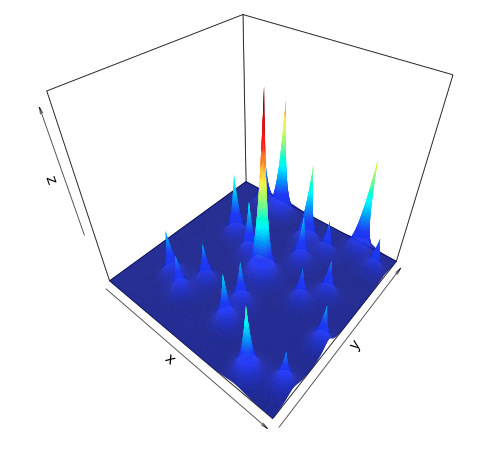
\includegraphics[width=0.4\textwidth]{Figures/Scaling/example_exp_mixture}
%\appcaption{Example of a synthetic density distribution obtained with the exponential mixture, with a grid of size $400\times 400$ and parameters $N=20$, $r_0=10$, $P_{max}=200$, $\alpha=0.5$, $\theta_C = 0.01$.}{Exemple de distribution synthétique}
%\label{fig:ex-distrib}
%\end{figure}
%%%%%%%%%%%%%%%%%%



%\begin{figure}
%\centering
%
%\caption{Validation of theoretical result through numerical simulation.}
%\label{fig:th_results}
%\end{figure}



%\paragraph{Random Perturbations}{Perturbations aléatoires}

%The simple model used is quite reducing for maximal densities and radius distribution. We aim to proceed to an empirical study of the influence of noise in the system by fixing $d_i^0$ and $r_i$ the following way :
%\begin{itemize}
%\item $d_i^0$ follows a reversed log-normal distribution with maximal value being a realistic maximal density
%\item Radiuses are computed to respect rank-size law and then perturbed by a white noise. \comment{(Florent)  pourquoi ?}
%\end{itemize}

%Results shown in Fig.~\ref{fig:random-density} are quantitatively different from previous one, as expected, but the same qualitative behavior is reproduced.


%\begin{figure}
%\centering

%\caption{Variation of exponents with variable origin density and radius.}
%\label{fig:random-density}
%\end{figure}



%\paragraph{Kernel Type}{Type de Noyau}

%We shall test the influence of the type of spatial kernel used on results. We can test gaussian kernels and quadratic kernels with parameters within reasonable ranges analog to the exponential kernel. %As shown in Fig.~\ref{fig:other-kernels}, we obtain the same qualitative results that is the significant variation of $\alpha(\theta)$ as a function of $\theta$.


%
%\begin{figure}
%\centering

%\caption{Scaling exponents for other kernels.}
%\label{fig:other-kernels}
%\end{figure}

%\paragraph{Two-parameters phase diagram}

%We introduce now a second spatial variable that has also an influence on the definition of urban entities, that is the proportion of actives working in city center, as done on empirical data in~\cite{cottineau2015scaling}. To simplify, it is used only to define urban parameter but assumed as having no influence on the local probability distribution of the amenity which stays the same function of the density. We write 

%\begin{figure}
%\centering

%\caption{Two parameters phase diagram.}
%\label{fig:two-params}
%\end{figure}

%%%%%%%%%%%%%%%%%%%%
%\subsection{Discussion}

%%%%%%%%%%%%%%%%%%%%
%\subsection{Conclusion}














%----------------------------------------------------------------------------------------


%%%%%%
% not really useful


%\newpage



%\section[Spatio-temporal Correlations][Correlations spatio-temporelles]{Linking dynamic and static spatio-temporal correlations under simplified assumptions}{Lien entre correlation spatio-temporelles statiques et dynamiques sous hypothèses simplifiées}
%\section{Spatio-temporal Correlations}{Correlations spatio-temporelles}



%\label{sec:app:spatiotempcorrs}


%\bpar{
%Space and Time are both crucial for the study of geographical systems when aiming to understand \emph{processes} (by definition dynamical~\cite{hypergeo}) 
% evolving in a \emph{spatial structure} in the sense of~\cite{dollfus1975some}. Space is more than coordinates for elements of the system, but a dimension in itself that drives interactions and thus system properties. Reading geographical systems from the point of view of \emph{spatio-temporal processes} emphasizes the fact that \emph{space actually matters}. Space and time are closely linked in such processes, and depending on the underlying mechanisms, one can expect to extract useful information from one on the other : in certain cases that we will investigate in this part, it is for example possible to learn about dynamics from static information. Spatio-temporal correlations approaches, linked to spatio-temporal dynamics, are present in very broad fields such as dynamical image processing (including video compression)~\cite{chalidabhongse1997fast,hansen2004accelerated,ke2007spatio}, target tracking~\cite{belouchrani1997direction,vuran2004spatio}, climate science~\cite{cressie1999classes}, Earth sciences~\cite{ma2002spatio}, city systems dynamics~\cite{hernando2015memory,pigozzi1980interurban}, among others.
%}{
%L'espace et le temps sont cruciaux pour l'étude des systèmes géographiques quand on cherche à comprendre les \emph{processus} (par définition dynamiques~\cite{hypergeo}) 
%\comment{(Florent)  c'est déjà une lecture, certes processus renvoie à une évolution,mais les échelles de temps du modèle/processus ne sont pas nécessairement les mêmes} 
%qui évoluent dans une structure spatiale au sens de~\cite{dollfus1975some}.
%\comment{(Florent) citer Cottineau ?}
%}
%
%\cite{cross1994spatiotemporal} : spatio-temporal chaos --> cf paper crutchfield
%
%
%The capture of neighborhood effects in statistical models is a wisely used practice in spatial statistics, as the technique of Geographically Weighted Regression illustrates~\cite{brunsdon1998geographically}. A possible interpretation among many definitions of spatial autocorrelation~\cite{griffith1992spatial} yields that by estimating a plausible characteristic distance for spatial correlations or auto-correlations, one can isolate independent effects between variables from effects due to neighborhood interactions\footnote{note that the formal link between models of spatial autocorrelation (see e.g. \cite{griffith2012advanced}) is not clear and should be further investigated}. The study of the spatial covariance structure is a cornerstone of advanced spatial statistics that was early formulated~\cite{griffith1980towards}. \comment{(Florent) cela semble tout de même loin du sujet ou alors il faut que tu expliques clairement}
% We propose now to study possible links between spatial and temporal correlations, using spatio-temporal covariance structure to infer information on dynamical processes.
%
%
%\subsection{Notations}{Notations}
%
%We consider a multivariate spatio-temporal stochastic process denoted by $\vec{Y}\left[\vec{x},t\right]$. At a given point $\vec{x}_0$ in space, we can define temporal covariance structure by
%\[
%\mathbf{C}_t (\vec{x}_0) = \Varb{\vec{Y}\left[\vec{x}_0, \cdot\right]}
%\]
%
%and spatial covariance structure at fixed time by
%\[
%\mathbf{C}_x (t) = \Varb{\vec{Y}\left[\cdot, t\right]}
%\]
%
%It is clear that these quantities will be in practice first ill-defined because of the difficulty in interpreting such a process by a spatio-temporal random variable, secondly highly non-stationary in space and time. We stay however at a theoretical level to gain structural knowledge,\comment{(Florent) sens ?}
% reviewing simple cases in which a formal link can be established.
%
%
%\subsection{Wave Equation}{Equation des Ondes}
%
%\comment{(Florent) pourquoi aborder cela ?}[cas idéal des STARMA, ondes d'innovation etc. : approche fondamentalement liée à l'analyse spatiale, mais bien plus complexe qu'une simple équation. justifie cette approche de lien spatio-temporel ?]
%
%In the case of propagating waves, there is an immediate link. Let assume that a wave equation if verified by ``deterministic'' parts of components
%
%\begin{equation}
%c^2 \cdot \partial^2_{t} \bar{Y}_i = \Delta \bar{Y}_i
%\end{equation}
%
%with $Y_i = \bar{Y}_i + \varepsilon_i$. If errors are uncorrelated and processes are stationary, we have then directly
%
%\begin{equation}
%\mathbf{C}_t \left[ \partial^2_t Y_i , \partial^2_t Y_j \right] = \frac{1}{c^2} \cdot\mathbf{C}_x \left[ \Delta Y_i , \Delta Y_j \right]
%\end{equation}
%
%This gives us however few insight on real systems as local diffusion, stationary assumptions and uncorrelated noises are far from being verified in empirical situations.
%
%\subsection{Fokker-Planck Equation}{Equation de Fokker-Planck}
%
%An other interesting approach may when the process verifies a Fokker-Planck equation on probabilities of the state of the system when it is given by its position (diffusion of particles in that case)
%
%\begin{equation}
%\partial_t P(x_i,t) = - d \cdot \partial_x P(x_i,t) + \frac{\sigma^2}{2} \partial^2_x P(x_i,t)
%\end{equation}
%
%With no cross-correlation terms in the Fokker-Planck equation, covariance between processes vanish. We have finally in that case only a relation between averaged spatial and temporal variances that brings no information to our question.
%
%\subsection{Master Equation}{Equation Maitresse}
%
%In the case of a master equation on probabilities of discrete states of the system
%
%\begin{equation}
%\partial_t \vec{P} = \mathbb{W} \vec{P}
%\end{equation}
%
%we have then for state $i$, $\partial_t P_i = \sum_j W_{ij}P_j$. As this relation is at a fixed time we can average in time to obtain an equation on temporal covariance. It is not clear how to make the link with spatial covariance as these will depend on spatial specification of discrete states. This question is still under investigation.
%
%
%\subsection{Consistent spatio-temporal sampling}{Echantillonnage spatial cohérent}
%
%In a more empirical way, we propose to not assume any contraint of process dynamics but to however investigate how the computation of spatial correlations can inform on temporal correlations. We try to formulate easily verifiable assumptions under which this is possible.
%
%We make the following assumptions on the spatio-temporal stochastic processes $Y_i\left[\vec{x},t\right]$ :
%\begin{enumerate}
%\item Local spatial autocorrelation is present and bounded by $l_{\rho}$ (in other words the processes are continuous in space) : at any $\vec{x}$ and $t$, $\left|\rho_{\norm{\Delta \vec{x}} < l_{\rho}}\left[Y_i (\vec{x}+\Delta \vec{x},t), Y_i (\vec{x},t) \right]\right| > 0$. \comment{(Florent) je ne comprends pas ce qui est écrit, qu'une abs soit > 0 ok, donc c'est autre mais quoi ?}[c'est le strict > 0 qui compte, c'est une façon de postuler que les processus sont continus à une certaine échelle fine]
%\item Processes are locally parametrized : $Y_i = Y_i\left[\alpha_i\right]$, where $\alpha_i (\vec{x})$ varies with $l_{\alpha}$, with $l_{\alpha} \gg l_{\rho}$.
%\item Spatial correlations between processes have a sense at an intermediate scale $l$ such that $l_{\alpha}\gg l \gg l{\rho}$.
%\item Processes covariance stationarity times scale as $\sqrt{l}$.
%\item Local ergodicity is present at scale $l$ and dynamics are locally chaotic.
%\end{enumerate}
%
%
%Assumptions one to three can be tested empirically and allow to compare spatial correlation estimated on spatial samplings at scale $l$. Assumption four is more delicate as we are precisely constructing this methodology because we have no temporal information on processes. It is however typical of spatial diffusion processes, and population or innovation diffusion should verify this assumption. \comment{(Florent)  cela devrait être un point de départ (expliquerait pourquoi ces modèles ; te ferait peut être en considérer d'autres}
% The last assumption can be tested if feasible space is known, by checking cribbing on image space on the spatial sample. Under these conditions, local spatial sampling is equivalent to temporal sampling and spatial correlation estimators provide estimator of temporal correlations.
%








%----------------------------------------------------------------------------------------

\newpage



\section{Generation of Correlated Synthetic Data}{Génération de données synthétiques corrélées}

\label{app:sec:syntheticdata}



%\stars

\textit{Cette section correspond à l'introduction et la formalisation de~\cite{raimbault2016generation}.}

\stars

\bpar{
Generation of hybrid synthetic data resembling real data to some criteria is an important methodological and thematic issue in most disciplines which study complex systems. Interdependencies between constituting elements, materialized within respective relations, lead to the emergence of macroscopic patterns. Being able to control the dependance structure and level within a synthetic dataset is thus a source of knowledge on system mechanisms. We propose a methodology consisting in the generation of synthetic datasets on which correlation structure is controlled. The method is applied in a first example on financial time-series and allows to understand the role of interferences between components at different scales on performances of a predictive model. A second application on a geographical system is then proposed, in which the weak coupling between a population density model and a network morphogenesis model allows to simulate territorial configurations. The calibration on morphological objective on european data and intensive model exploration unveils a large spectrum of feasible correlations between morphological and network measures. We demonstrate therein the flexibility of our method and the variety of possible applications.
}{
La génération de données synthétiques hybrides similaires à des données réelles présente des enjeux méthodologiques et thématiques pour la plupart des disciplines dont l'objet est l'étude de systèmes complexes. Comme l'interdépendance entre les éléments constitutifs d'un système, matérialisée par leur relations, conduit à l'émergence de ses propriétés macroscopiques, une possibilité de contrôle de l'intensité des dépendances dans un jeu de données synthétiques est un instrument de connaissance du comportement du système. Nous proposons une méthodologie de génération de données synthétiques hybrides sur lequel la structure de correlation est contrôlée. La méthode est illustrée sur des séries temporelles financières en~\ref{app:sec:syntheticdata-finance} et permet l'étude de l'interférence entre composantes à différentes fréquences sur la performance d'un modèle prédictif, en fonction des correlations entre composantes à différentes échelles. La section~\ref{sec:correlatedsyntheticdata} propose par ailleurs une application à un système géographique, dans laquelle le couplage faible d'un modèle de distribution de densité de population avec un modèle de génération de réseau permet la simulation de configurations territoriales. L'exploration intensive du modèle permet l'obtention d'un large spectre de valeurs pour la matrice de correlation entre mesures morphologiques et mesures du réseau. On démontre ainsi les possibilités d'applications variées et les potentialités de la méthode.
}




\subsection{Context}{Contexte}

\bpar{

The use of synthetic data, in the sense of statistical populations generated randomly under constraints of patterns proximity to the studied system, is a widely used methodology, and more particularly in disciplines related to complex systems such as therapeutic evaluation~\cite{abadie2010synthetic}, territorial science~\cite{moeckel2003creating,pritchard2009advances}, machine learning~\cite{bolon2013review} or bio-informatics~\cite{van2006syntren}. It can consist in data desegregation by creation of a microscopic population with fixed macroscopic properties, or in the creation of new populations at the same scale than a given sample, with criteria of proximity to the real sample. These criteria will depend on expected applications and can for example vary from a restrictive statistical fit on given indicators, to weaker assumptions of similarity in aggregated patterns. In the case of chaotic systems, or systems where emergence plays a strong role, a microscopic property does not directly imply given macroscopic patterns, which reproduction is indeed one aim of modeling and simulation practices in complexity science. With the rise of new computational paradigms~\cite{arthur2015complexity}, data (simulated, measured or hybrid) shape our understanding of complex systems. Methodological tools for data-mining and modeling and simulation (including the generation of synthetic data) are therefore crucial to be developed.
}{
L'utilisation de données synthétiques, au sens de populations statistiques d'individus générées aléatoirement sous la contrainte de reproduire certaines caractéristiques du système étudié, est une pratique méthodologique largement répandue dans de nombreuses disciplines, et particulièrement pour des problématiques liées aux systèmes complexes, telles que par exemple l'évaluation thérapeutique~\cite{abadie2010synthetic}, l'étude des systèmes territoriaux~\cite{moeckel2003creating,pritchard2009advances}, l'apprentissage statistique~\cite{bolon2013review} ou la bio-informatique~\cite{van2006syntren}. Il peut s'agir d'une désagrégation par création d'une population au niveau microscopique présentant des caractéristiques macroscopiques données, ou bien de la création de nouvelles populations au même niveau d'agrégation qu'un échantillon donné avec un critère de ressemblance aux données réelles.  Le niveau de ce critère peut dépendra des applications attendues et peut par exemple aller de la fidélité des distributions statistiques pour un certain nombre d'indicateurs à des contraintes plus faibles de valeurs pour des indicateurs agrégés, c'est-à-dire l'existence de motifs macroscopiques similaires. Dans le cas de systèmes chaotiques ou présentant de fortes caractéristiques d'émergence, une contrainte microscopique n'implique pas nécessairement le respect des motifs macroscopiques, et arriver à les reproduire est justement un des enjeux des pratiques de modélisation et simulation en sciences de la complexité. La donnée, qu'elle soit simulée, mesurée ou hybride est au coeur de l'étude des systèmes complexes de par la maturation de nouvelles approches computationelles~\cite{arthur2015complexity}, il est donc essentiel d'étudier des procédures d'extraction d'information des données (fouille de données) et de simulation d'une information similaire (génération de données synthétiques).
}




\bpar{
Whereas first order (in the sense of distribution moments) is generally well used, it is not systematic nor simple to control generated data structure at second order, i.e. covariance structure between generated variables. Some specific examples can be found, such as in~\cite{ye2011investigation} where the sensitivity of discrete choices models to the distributions of inputs and to their dependance structure is examined. It is also possible to interpret complex networks generative models~\cite{newman2003structure} as the production of an interdependence structure for a system, contained within link topology. We introduce here a generic method taking into account dependance structure for the generation of synthetic datasets, more precisely with the mean of controlled correlation matrices.
}{
Si le premier ordre est de manière générale bien maîtrisé, il n'est pas systématique ni aisé de contrôler le second ordre, c'est-à-dire les structures de covariance entre les variables générées, même si des exemples spécifiques existent, comme dans~\cite{ye2011investigation} où la sensibilité des sorties de modèles de choix discrets à la forme des distributions des variables aléatoires ainsi qu'à leur structures de dépendance. Il est également possible d'interpréter les modèles de génération de réseaux complexes~\cite{newman2003structure} comme la création d'une structure d'interdépendance au sein d'un système, représentée par la topologie des liens. Nous proposons ici une méthode générique prenant en compte l'interdépendance lors de la génération de données synthétiques, sous la forme de correlations.
}



\bpar{
Domain-specific methods aforementioned are too broad to be summarized into a same formalism. We propose a framework as generic as possible, centered on the control of correlations structure in synthetic data.
}{
L'ensemble des méthodologies mentionnées en introduction sont trop variées pour être résumées par un même formalisme. Nous proposons ici une formulation générique ne dépendant pas du domaine d'application, ciblée sur le contrôle de la structure de correlation des données synthétiques.
}


%%%%%%%%%%%%%
\subsection{Formalization}{Formalisation}


\bpar{
Let $\vec{X}_I$ a multidimensional stochastic process (that can be indexed e.g. with time in the case of time-series, but also space, or discrete set abstract indexation). We assume given a real dataset $\mathbf{X}=(X_{i,j})$, interpreted as a set of realizations of the stochastic process. We propose to generate a statistical population $\mathbf{\tilde{X}}=\tilde{X}_{i,j}$ such that
\begin{enumerate}
\item a given criteria of proximity to data is verified, i.e. given a precision $\varepsilon$ and an indicator $f$, we have $\norm{f(\mathbf{X})-f(\mathbf{\tilde{X}})} < \varepsilon$
\item level of correlation is controlled, i.e. given a matrix $R$ fixing correlation structure (symmetric matrix with coefficients in $[-1,1]$ and unity diagonal), we have $\hat{\Var{}}\left[(\tilde{X}_i)\right] = \Sigma R \Sigma$, where the standard deviation diagonal matrix $\Sigma$ is estimated on the synthetic population.
\end{enumerate}
}{
Soit un processus stochastique multidimensionnel $\vec{X}_I$ (l'ensemble d'indexation pouvant être par exemple le temps dans le cas de séries temporelles, l'espace, ou une indexation quelconque). On se propose, à partir d'un jeu de réalisations $\mathbf{X}=(X_{i,j})$, de générer une population statistique $\mathbf{\tilde{X}}=\tilde{X}_{i,j}$ telle que
\begin{enumerate}
\item d'une part un certain critère de proximité aux données est vérifié, i.e. étant donné une précision $\varepsilon$ et un indicateur $f$, $\norm{f(\mathbf{X})-f(\mathbf{\tilde{X}})} < \varepsilon$
\item d'autre part le niveau de correlation est controlé, i.e. étant donné une matrice fixant une structure de covariance $R$, $\Varb{(\tilde{X}_i)} = R$, où la matrice de variance/covariance est estimée sur la population synthétique.
\end{enumerate}
}


\bpar{
The second requirement will generally be conditional to parameter values determining generation procedure, either generation models being simple or complex ($R$ itself is a parameter). Formally, synthetic processes are parametric families $\tilde{X}_i[\vec{\alpha}]$. \comment{explicit the fact that real data may come out of different parameter values ?}
We propose to apply the methodology on very different examples, both typical of complex systems : financial high-frequency time-series and territorial systems. We illustrate the flexibility of the method, and claim to help building interdisciplinary bridges by methodology transposition and reasoning analogy. In the first case, proximity to data is the equality of signals at a fundamental frequency, to which higher frequency synthetic components with controlled correlations are superposed. It follows a logic of hybrid data for which hypothesis or model testing is done on a more realistic context than on purely synthetic data. This example that has no thematic link with the thesis, is presented in Appendix~\ref{app:syntheticdata}. In the second case, morphological calibration of a population density distribution model allows to respect real data proximity. Correlations of urban form with transportation network measures are empirically obtained by exploration of coupling with a network morphogenesis model. The control is in this case indirect as feasible space is empirically determined.
}{
La satisfaction du deuxième point sera généralement conditionnée par la valeur de paramètres, dont dépendra la procédure de génération, qu'il s'agisse de modèles simples ou complexes. Formellement, les processus synthétiques sont des familles paramétriques $\tilde{X}_i[\vec{\alpha}]$. Nous proposons de décliner cette méthode sur deux exemples très différents mais tous deux typiques des systèmes complexes : des séries temporelles financières à haute fréquence, et les systèmes territoriaux. On illustre ainsi la flexibilité de la logique, ouvrant des portes interdisciplinaires par l'exportation de méthodes ou raisonnements par exemple. Dans le premier cas, la proximité aux données est l'égalité des signaux à une fréquence fondamentale, auxquels on superpose des composantes synthétiques dont il est facile de contrôler le niveau de correlation. On se place dans une logique de données hybrides, pour tester des hypothèses ou modèles dans un contexte plus proche de la réalité que sur des données purement synthétiques. Cet exemple est présenté en Appendice~\ref{app:sec:syntheticdata-finance}. Dans le deuxième cas, la calibration morphologique d'un modèle de distribution de densité de peuplement permet de respecter le critère de proximité aux données. Les correlations de la forme urbaine avec celle d'un réseau de transport sont ensuite obtenues empiriquement par exploration du couplage avec un modèle de génération de réseau. Leur contrôle est dans ce cas indirect puisque constaté empiriquement.
}



\stars


%%%%%
% from space matters

%\paragraph{An alternative view : synthetic data}{Une vue alternative: données synthétiques}

%Let $M_{m}$ a stochastic model of simulation, which inputs are to simplify initial conditions $D_0$ and parameters $\vec{\alpha}$, and output $M_{m}\left[\vec{\alpha},D_0\right](t)$ at a given time $t$. We assume that it is partially data-driven in the sense that $D_0$ is supposed to represent a real situation at a given time, and model performance is measured by the distance of its output at final time to the real situation at the corresponding time, i.e. error function is of the form $\norm{\Eb{\vec{g}(M_{m}\left[\vec{\alpha},D_0\right](t_f))}-\vec{g}(D_f)}$ where $\vec{g}$ is a deterministic field corresponding to given indicators.


%Evaluating the model on real data is rapidly limited in control possibilities, being restricted to the search of datasets allowing natural control groups. Furthermore, statistical behaviors are generally poorly characterized because of the small number of realizations. Working with synthetic data first allows to solve this issue of robustness of statistics, and then gives possibilities of control on some ``meta-parameters'' in the sense described before.

%Some remarks can be made on the approach: We can ask what knowledge are brought by adding the upstream model, rather than exploring a large set of initial geometries ? To obtain a sufficiently large set of initial configuration, one quickly needs a model to generate them ; in that case a quasi-random generation followed by a filtering on morphological constraint will be a morphogenesis model, which parameters are the ones of the generation and the filtering methods. Furthermore, as detailed further, the determination of the derivative of the downstream model is made possible by the coupling and knowledge of the upstream model.
%\comment{(Florent) est-ce important pour la thèse ?}
%If statistical noise is added by coupling models, indeed repetitions needed for convergence are indeed larger as the final expectance has to be determined by repeating on the first times the second model ; but it is exactly the same as exploring directly many configuration, to obtain statistical robustness in that case one must repeat on similar configurations.
%Finally, if complexity is added by coupling models, coupling is simple and no complexity is thus added.

%\comment{link between synthetic data and model coupling ?}

% necessity of separation of scales and ontologies for space matters to work ? not necessarily (deleted paragraph). think to that.
















%%%%%%%%%%%%%%%%%%%%%%%%%%%%%






\cleardoublepage % Empty page before the start of the next part

%------------------------------------------------

\ctparttext{This part provides building blocks for the final objective of constructing models of co-evolution. These contain both stylized facts from empirical analyses and toy and hybrid modeling. They correspond to three distinct components of our overall construction: first analyses at the micro-scale confirming the chaotic and non-stationary nature of interactions between networks and territories, secondly a morphogenetic vision of these that corresponds roughly to a meso-scale, and finally an application of the evolutive urban theory at the macro-scale.}


% Part II : Empirical analysis / Toy-modeling
% Part 2 set up the elementary bricks for further work
%\part{Architecture and Building Bricks : preparing the construction}
\part{Briques Elémentaires}



%%%%%%%%%%%%%%%
% 1) Micro-level




% Chapter 

%\chapter{Interactions at the Micro Level}{Interactions au niveau microscopique} % Chapter title

\chapter{Echelles et Ontologies}

\label{ch:micro} % For referencing the chapter elsewhere, use \autoref{ch:name} 

%----------------------------------------------------------------------------------------


%\headercit{}{}{}


\bigskip



La richesse des interactions entre réseaux et territoires, développée dans le Chapitre~\ref{ch:thematic}, est que celle-ci se produisent à différentes échelles, entre ces échelles, et par des intermédiaires très variés, au sens des agents ou structures impliquées mais aussi de leur caractéristiques, ceux-ci allant de la congestion des réseaux aux dynamiques sur le temps long en passant par les re-localisations des activités par exemple. Le cas de Zhuhai développé en~\ref{sec:casestudies} illustre la complexité d'une trajectoire locale et régionale, d'une bifurcation politique induisant l'instauration de la Zone Economique Spéciale par \noun{Xi Jinping} conditionnée à une bifurcation historique bien plus ancienne liée à la colonisation européenne qui a conduit à l'existence de Macao\comment[FL]{mal dit}, à une bifurcation géographique\comment[FL]{trop simple, toutes les bifurcations sont a la fois geographique, historique, etc.} en terme d'accessibilité régionale et une nouvelle position centrale de la ville dans la Mega-city Region du Delta de la Rivière des Perles. Nous avons dans le chapitre précédent étudié empiriquement les manifestations morphologiques des interactions à l'échelle mesoscopique\comment[FL]{c'est dans ce chapitre qu'il faut discuter de ces echelles, pas avant}, mais également mis en évidence des effets de structure à cette même échelle sur un temps long dans le cas de l'Afrique du Sud. Quelle échelle minimale est-il pertinent de considérer, autrement dit l'étude de l'échelle microscopique peut-elle nous apporter de l'information ? Et peut-on clarifier certaines ontologies, ou au moins un certain degré de précision ou de complexité requis dans celles-ci ? Ce chapitre cherche à répondre à ces interrogations par le biais d'études empiriques. Ainsi, nous tentons de préciser itérativement la structure des modèles futurs, mais aussi leur non-structure.


Dans une première section~\ref{sec:transportationequilibrium}, nous explorons empiriquement un jeu de données à l'échelle microscopique sur le trafic routier en Ile-de-France, en ayant notamment à l'esprit la notion d'équilibre des flux de trafic qui est une hypothèse particulièrement répandue dans la modélisation du trafic. Nous démontrons que cet équilibre n'a aucun fondement empirique\comment[FL]{et alors ? en quoi est-ce problematique ?}, et que les trajectoires microscopiques du système sont chaotiques. Cela nous permettra d'une part de conforter nos choix épistémologiques de modèle loin de l'équilibre typique d'une appréhension de la complexité, d'autre part de confirmer que cette échelle n'est pas pertinente. Nous continuons sur le traffic routier dans une deuxième section~\ref{sec:energyprice}, en nous concentrons sur la composante du prix de transport via le proxy du prix de vente du carburant, et ces liens potentiels avec les caractéristiques socio-économiques des territoires, dans le cas des Etats-Unis avec une granularité spatiale au comté et temporelle à la journée. Nous obtenons le résultat assez inattendu des deux échelles endogènes proprement définies, correspondant aux échelles mesoscopique et macroscopique, mais aussi la mise en évidence de la superposition de processus de gouvernance à des processus locaux. Enfin, la dernière section~\ref{sec:grandparisrealestate} applique la méthode d'identification de causalités développée en~\ref{sec:causalityregimes} au différents projets de transport du Grand Paris et démontre des potentiels effets d'annonce des projets de transport sur la croissance de la population, confirmant la pertinence d'une échelle d'agrégation au moins mesoscopique et de se concentrer sur des variables territoriales relativement basiques.



\stars


\bpar{
\textit{This chapter is entirely adapted from diverse papers: section \ref{} was published}
}{
\textit{Ce chapitre est entièrement adapté de divers articles: la section~\ref{sec:transportationequilibrium} a été publiée en anglais comme \cite{raimbault2017investigating}; la section~\ref{sec:energyprice} également en anglais en collaboration avec \noun{A. Bergeaud} comme \cite{raimbault2017cost}; la section \ref{sec:grandparisrealestate} correspond à la partie d'application de \cite{raimbault2017identification}.}
}




%----------------------------------------------------------------------------------------









%%%%%%%%%%%%%%%



%%%%%%%%%%%%%%%
% 2) Urban Morphogenesis



% Chapter 

%\chapter{Urban Morphogenesis}{Morphogenèse Urbaine} % Chapter title
\chapter{Morphogenèse Urbaine}

\label{ch:morphogenesis} % For referencing the chapter elsewhere, use \autoref{ch:name} 

%----------------------------------------------------------------------------------------

%\headercit{}{}{}

%\bigskip


Il est bien établi en géographie l'importance des relations spatiales et de la mise en réseau, comme le formule \noun{Tobler} par sa ``première loi de la géographie''~\cite{tobler2004first}\comment[FL]{la citer}.\comment[CC]{phrase a reformuler: les relations spatiales ... sont bien etablies en geo, et comme le prouve par ex. la premiere loi de la geo de tobler "..."} Nous l'avons mis en évidence pour les relations entre réseaux et territoires par exemple en section~\ref{sec:interactiongibrat}. Toutefois, les travaux sur la non-stationnarité et la non-ergodicité, ainsi que la mise en valeur d'échelles locales endogènes, suggèrent une certaine pertinence à l'idée de sous-système relativement indépendant, au sens où il serait possible d'isoler certaines règles locales régissant celui-ci étant fixés certains paramètres exogène\comment[CC]{s} capturant justement les relations avec d'autres sous-systèmes\comment[CC]{pas clair. plutot faire 3 phrases sinon on perd completement le sens}. Cette question porte à la fois sur l'échelle d'espace, de temps, mais aussi sur les éléments concernés. Reprenons un exemple concret de terrain déjà évoqué en Chapitre~\ref{ch:thematic}: la laborieuse mise en place du tramway de Zhuhai. L'impact du retard de la mise en place et la remise en question de futures lignes, dus à un problème technique inattendu lié à une technologie de transfert de courant par troisième rail importée d'Europe qui n'avait jamais été testée dans les conditions climatiques locales, assez exceptionnelles en termes d'humidité, aura une nature très différentes selon l'échelle et les agents considérés\comment[CC]{hierarchise cette phrase: les details entre parentheses et l'info principale mise en valeur "le retard et l'incertitude affecte differents acteurs differement}. Le manque de coordination générale entre transports et urbanisme laisse supposer que les dynamiques urbaines en terme\comment[CC]{s} de populations et d'emplois y sont relativement insensibles à court terme\comment[FL]{sens ?}. Le Bureau des Transports de la Municipalité ainsi que le bureau technique Européen ont pu subir des répercussions politiques et économiques bien plus graves\comment[FL]{$\sim$}\comment[CC]{quel rapport? on est toujours a Zhuhai ou pas?}. D'autre part, que ce soit à Zhongshan, Macao ou Hong-Kong le problème a une repercussion quasi-nulle\comment[CC]{c'est un resultat ou une supposition? Avant de generaliser, a ta place, j'interpreterais cette info d'abord: dans ces 3 villes, pas d'incidence car connexion faible et diffferents sous-systemes qui amortissent}. Généralisant au système de transport local, celui-ci peut être relativement bien isolé des systèmes voisins ou à plus grande échelle\comment[CC]{supprimer "ou a plus grande echelle}, et donc ses relations avec la ville considérée dans un contexte local. On supposera à la fois une certaine forme de stationnarité locale (``régime urbain local'') mais aussi une certaine indépendance avec l'extérieur. Dans ce cadre, son auto-organisation locale impliquera nécessairement des relations fortes entre forme et fonction, de par la distribution spatiale des fonctions urbaines mais aussi car \emph{la forme fait la fonction} dans certains cas de figure, au sens des motifs d'utilisation entièrement conditionnés à cette forme\comment[CC]{je vois pas le lien avec les phrases precedentes}. Le type de raisonnement que nous avons esquissé mobilise les éléments essentiels propres à l'idée de \emph{morphogenèse urbaine}. Nous allons dans ce chapitre clarifier sa définition et montrer les potentialité\comment[CC]{s} qu'elle donne pour éclairer les relations entre réseaux et territoires. La morphogenèse, qui a été importée de la biologie vers de nombreux champs, a dans chaque cas ouvert des voies pour l'étude des systèmes complexes propres à ce champ selon un point particulier. Il est important de noter que le monument qu'est la Théorie des Catastrophes de \noun{René Thom} introduit une façon originale de comprendre la différentiation qualitative et donc la morphogenèse. Cette théorie, très mal comprise \comment[CC]{par qui? est-ce que c'est important dans ton argumentation ici? sinon ca fait un peu pedanterie gratuite}, contient un potentiel d'application immense aux problèmes qui nous concernent, comme l'a effleuré \comment[CC]{id} \noun{Durand-Dastès}~\cite{durand2003geographes} en évoquant la systèmogenèse, que nous développerons en ouverture. Dans un premier temps, un effort d'épistémologie par des points de vue complémentaires de plusieurs disciplines permet d'éclairer la nature de la morphogenèse dans la section~\ref{sec:interdiscmorphogenesis}. Cela permet de clarifier le concept en lui donnant une définition bien précise, distincte de celle de l'auto-organisation, qui appuie les relations causales circulaires entre forme et fonction. Nous explorons ensuite un modèle simple de morphogenèse urbaine, basé sur la densité de population seule, à l'échelle mesoscopique, dans la section~\ref{sec:densitygeneration}. La démonstration que les processus abstraits d'agrégation et de diffusion sont suffisants pour reproduire l'ensemble des formes d'établissements humains en Europe, en utilisant les résultats de~\ref{sec:staticcorrelations}, confirme la pertinence de l'idée de morphogenèse pour la modélisation à certaines échelles et pour certains aspects\comment[CC]{lesquels? si tu ne les mentionnes pas, ca n'apporte aucune information}. Ce modèle est ensuite couplé de manière séquentielle à un module de morphogenèse de réseau dans la section~\ref{sec:correlatedsyntheticdata}, afin d'établir un espace faisable \comment[CC]{faisable? ou bien plutot theorique / potentiel / possible} des correlations statiques entre indicateurs de forme urbaine et indicateurs de réseau, qui sont comme on l'a vu précédemment un témoin des relations locales entre réseaux et territoires \comment[CC]{cool}. Celui-ci s'avère relativement large, ce qui confirmera l'utilisation de ce type de modèle de manière fortement couplée par la suite\comment[CC]{pourquoi? il faut expliquer tes conclusions car ca n'est pas evident}.




\stars


\textit{Ce chapitre est composé de divers travaux. La première section est adaptée d'un travail en anglais en collaboration avec \noun{C. Antelope}, \noun{L. Hubatsch} et \noun{J.M. Serna} à la suite de l'école d'été 2016 du Santa Fe Institute~\cite{antelope2016interdisciplinary}; la deuxième section est traduite de~\cite{} \comment[CC]{pas de ref.}; et enfin la troisième section a été écrite pour les Actes des Journées de Rochebrune 2016~\cite{raimbault2016generation}.}



\comment[CC]{Attention. Les parties traduites sont tres claires et avec un niveau de langage soigne, tandis que les introductions / transitions sont brouillonnes et touffues. Il faudrait harmoniser le tout, c'est a dire surtout fluidifier les transitions qui sont la partie en propre de ton manuscript de these, le reste etant deja publie ailleur}





%----------------------------------------------------------------------------------------










%%%%%%%%%%%%%%%




%%%%%%%%%%%%%%%
% 3) Evolutive Urban Theory



% Chapter 

%\chapter{Evolutive Urban Theory}{Théorie Evolutive Urbaine} % Chapter title
\chapter{Théorie Evolutive Urbaine}

\label{ch:evolutiveurban} % For referencing the chapter elsewhere, use \autoref{ch:name} 

%----------------------------------------------------------------------------------------


%\headercit{Mais ce n'est pas une question d'{\^a}ge, de chiffres et de stats\\ Moi je te parle surtout de rage, de kif et d'espoir}{Youssoupha}{\textit{, Esperance de Vie}}

%\headercit{}{}{}


\bigskip



\todo{quel niveau de description de la théorie évolutive ici ? insérer l'étude méthodes mixtes en dernier opening : illustration/construction du cadre de connaissances.}


%As this quote suggests, a purely quantitative view of the world makes no sense without qualitative counterbalancing. More precisely, we argue that the \textit{clich{\'e}} of an opposition between quantitative and qualitative analysis is an illusion. No distinct boundary exists between both. We propose to call quantitative any process involving computation by a Turing machine, whereas the qualitative will be for us the modeling design process and its interpretations. \comment{(Florent) je ne sais pas si je rangerais l'interprétation dans le qualitatif ; ok pour dire (même si connait rien en machine de Turing) que certaines observations via ``Turing'' peuvent s'appeler quantitatives. mais dans un cas comme dans l'autre, ensuite, il faut interpreter}
% Therefore both are necessarily closely interlaced in any of our approaches. In particular concerning the construction and the validation or refutation of our theory, empirical analysis on real case studies, implying the extraction and qualification of stylized facts, follows that schema.

% articulation with theoretical questions
% articulation with modeling

%\comment{(Florent) Entre cette phrase (next) et le détail projet par projet, il serait bien que tu te positionnes sur le cadre analytique général, justement comme tu l'introduis en parlant des objets et des échelles}

%We propose in this chapter various empirical analysis on different objects at different scales. A first section begins the examination of static spatial correlations between morphological measures of population density and road network measures on Europe at a 500m resolution. Applying last section of the methodological chapter should provide information on typical spatial scales of interaction between these indicators \comment{(Florent) à quel niveau se situe l'indicateur ?}
% of territory and network and on dynamical correlations between these. These computation furthermore provide empirical measures on which one model will be calibrated. We then describe a roadmap for statistical analysis on dynamical data of interactions for Bassin Parisien in the last fifty years. An other project using Real Estate transaction data for Parisian Metropolitan Region aim at seeking early warning of network breakdowns. We finally describe potential analyses on South African historical data. \comment{(Florent) ah bon et maintenant la Chine ? :) }









%%%%%%%%%%%%%%%





%%%%%%%%%%%%%%%
% Stylized facts : empirical analysis


% Chapter 

\section{Empirical Analysis : Insights from Stylized Facts}{Analyse Empirique} % Chapter title

\label{ch:empirical} % For referencing the chapter elsewhere, use \autoref{ch:name} 

%----------------------------------------------------------------------------------------


\headercit{Mais ce n'est pas une question d'{\^a}ge, de chiffres et de stats\\ Moi je te parle surtout de rage, de kif et d'espoir}{Youssoupha}{\textit{, Esperance de Vie}}


\bigskip


%  plan : 

%  1) static morphological analysis : requires a formal link between temporal and spatial correlations ?  -- typology etc can already be interesting --


%  2) presentation of BP case study

%  3) base Bien

%  4) Work with Solène



%----------------------------------------------------------------------------------------


As this quote suggests, a purely quantitative view of the world makes no sense without qualitative counterbalancing. More precisely, we argue that the \textit{clich{\'e}} of an opposition between quantitative and qualitative analysis is an illusion. No distinct boundary exists between both. We propose to call quantitative any process involving computation by a Turing machine, whereas the qualitative will be for us the modeling design process and its interpretations. \comment{(Florent) je ne sais pas si je rangerais l'interprétation dans le qualitatif ; ok pour dire (même si connait rien en machine de Turing) que certaines observations via ``Turing'' peuvent s'appeler quantitatives. mais dans un cas comme dans l'autre, ensuite, il faut interpreter}
 Therefore both are necessarily closely interlaced in any of our approaches. In particular concerning the construction and the validation or refutation of our theory, empirical analysis on real case studies, implying the extraction and qualification of stylized facts, follows that schema.

% articulation with theoretical questions
% articulation with modeling

\comment{(Florent) Entre cette phrase (next) et le détail projet par projet, il serait bien que tu te positionnes sur le cadre analytique général, justement comme tu l'introduis en parlant des objets et des échelles}

We propose in this chapter various empirical analysis on different objects at different scales. A first section begins the examination of static spatial correlations between morphological measures of population density and road network measures on Europe at a 500m resolution. Applying last section of the methodological chapter should provide information on typical spatial scales of interaction between these indicators \comment{(Florent) à quel niveau se situe l'indicateur ?}
 of territory and network and on dynamical correlations between these. These computation furthermore provide empirical measures on which one model will be calibrated. We then describe a roadmap for statistical analysis on dynamical data of interactions for Bassin Parisien in the last fifty years. An other project using Real Estate transaction data for Parisian Metropolitan Region aim at seeking early warning of network breakdowns. We finally describe potential analyses on South African historical data. \comment{(Florent) ah bon et maintenant la Chine ? :) }















%%%%%%%%%%%%%%%




%%%%%%%%%%%%%%%
% Toy modeling : density model / correlated synthetic data


% Chapter 

\section{Modeling}{Modélisation} % Chapter title

\label{ch:modeling} % For referencing the chapter elsewhere, use \autoref{ch:name} 





%----------------------------------------------------------------------------------------

\headercit{Do or do not. There is no try.}{Yoda}{}


\bigskip


One does not simply \emph{try} to model something. On that point personal experience confirms indeed that point, as I remember as an early Master student giving in to the call of incautious agent-based modeling, \comment{(Florent) pas forcément approprié dans une thèse}
 naively thinking that integrated models of any aspect of an urban system could be constructed, producing numerous NetLogo code lines to build a gaz factory with unfounded internal processes, an extremely poor external validation and no internal validation. This was a try and therefore a step towards the dark side of models bricolage. The construction of a computational model of simulation is a rigorous exercise that one can not improvise, as much as statistical modeling. Recent progresses in the field~\cite{banos2013pour} help to that purpose, and modular model construction and validation is one tool useful to avoid becoming lost in shady places.

We propose in this chapter simple modeling experiments, conceived to be preliminaries for more elaborated tests of our theory. We begin with a simple diffusion-aggregation model of urban growth as a relatively small scale. Beginning with simple assumptions does not mean a non-rigorous exploration of the model, that is therefore explored and calibrated on real data. The fact that we reproduce existing urban forms \comment{(Florent) oui mais ce n'est pas du tout un problème pour ta thèse. Ta thèse porte sur FU $\leftrightarrow$ Réseaux ; le fait qu'on puisse faire des modèles forme urbaine purs (avec mécanismes abstraits) et idem pour les réseaux d'ailleurs ne change rien à l'affaire. tout tes modèles ne doivent pas viser à reproduire FU \& réseau mais à reproduire FU $\leftrightarrow$ Réseaux}
 without the use of networks suggest either the total absence of network influence at this scale, or its very strong influence yielding apparent random effects that disappear in average calibration. We propose then to simply couple this model with a network generation heuristic in order to study feasible correlations between morphology and network. The absence of coupled calibration \comment{(Florent) pourquoi ? remarque tu dis le contraire là ?}
  avoids to draw empirical conclusion but the method is satisfying in itself as it permits the generation of synthetic territorial configurations where correlation structure is controlled. We finally describe a project of benchmark of diverse heuristic models for network generation.

















%%%%%%%%%%%%%%%




\cleardoublepage % Empty page before the start of the next part




%------------------------------------------------

\ctparttext{The buildings bricks, methods and tools are mainly set up for the culminating part of our work, which consists in the construction of models of co-evolution at different scales.}


% Part III : co-evolution models
\part{Synthesis: Construction}





%%%%%%%%%%%%%%%
% introduction of part III




%\chapter*{Introduction}{Introduction}

% to have header for non-numbered introduction
%\markboth{Introduction}{Introduction}


%\headercit{}{}{}


\todo{Plutôt en Conclusion Partie III : Towards operational Models : what is possible ; what is desirable ; etc.}




\bigskip




\begin{table}
\begin{tabular}[6pt]{c|c|c|c|c}
Processus & Analyse Empirique & Echelles & Type \textit{find a typology of processes} & Modèle \\\hline
Attachement préférentiel & & Croissance Urbaine & & \\\hline
Diffusion/Etalement & & Forme Urbaine & &\\\hline
Accessibilité  & & Réseau / Ville & & \\\hline
Gouvernance des Transports & & & &\\\hline
Flux direct  & & & &\\\hline
Flux indirect/Effet tunnel \textit{c'est le même processus, vu sous un angle différent : l'effet tunnel est l'absence de nw feedback} & & & &\\\hline
Centralité de proximité (accessibilité : generalisation) & & & &\\\hline
Centralité de Chemin (correspond aux flux indirect : différents niveaux de généralité / sous-processus-sous-classif ?) & & & &\\\hline
Proximité au réseau & & & &\\\hline
Distance au centre (similar to agrégation ?) & & & RBD &\\\hline
\end{tabular}
\caption{Description des différents processus pris en compte dans les modèles de co-évolution}{}
\end{table}


\comment{faire le même tableau pour les modèles existants : vue plus large de l'ensemble des processus. pour chacun de ces modèles et de nos modèles, lister tous les processus potentiels ; faire une typologie ensuite. Q : typologie différente d'une pure empirique ? a creuser, et peut être intéressant dans le cadre du knowledge framework, comme illustration coevol connaissances.}




\paragraph{}{Echelles et processus}

Partant des hypothèses tirées des enseignements empiriques et théoriques, on postulera \emph{a priori} que certaines échelles privilégient certains processus, par exemple que la forme urbaine aura une influence au niveaux micro et mesoscopiques, tandis que les motifs émergeant des flux agrégés entre villes au sein d'un système se manifesteront au niveau macroscopique. Toutefois la distinction entre échelles n'est pas toujours si claire et certains processus tels la centralité ou l'accessibilité sont de bons candidats pour jouer un rôle à plusieurs échelles\footnote{on entend ici par ``jouer un rôle'' avoir une autonomie propre à l'échelle correspondante, c'est à dire qu'ils émergent \emph{faiblement}  des niveaux inférieurs.}% TODO somewhere clarification and discussion on definitions of emergence, Bedau etc.
 : il s'agira par la modélisation d'également tester ce postulat, par comparaison des processus nécessaires et/ou suffisants dans les familles de modèles à différentes échelles que nous allons mettre en place, en gardant à l'esprit des possibles développements vers des modèles multi-scalaires dans lesquels ces processus intermédiaires joueraient alors un rôle crucial. % TODO : multi-scale modeling : who does some and how much ?








% introduction de la partie 

\section*{A Roadmap for an Operational Family of Models of Coevolution}{Vers des Modèles Opérationnels de Coevolution} % Chapter title

\label{ch:operational}

%----------------------------------------------------------------------------------------

As previously stated, one of our principal aims is the validation of the network necessity assumption, that is the differentiating point with a classic evolutive urban theory. To do so, toy-model exploration and empirical analysis will not be enough as hybrid models are generally necessary to draw effective and well validated conclusions. We briefly give an overview of planned work in the following, that will be the conclusion of this Memoire.



%----------------------------------------------------------------------------------------



\section*{Objectives}{Objectifs}


We expect to product \emph{models of coevolution}, \comment{(Florent) expliciter la différence avec ce que tu as fait jusque là}
 with the emphasis on processes of coevolution, to directly confront the theory. They will be necessary a flexible family because of the variety of scales and concrete cases we can include and we already began to explore in preliminary studies. Processes already studied can serve either as a thematic bases for a reuse as building bricks in a multi-modeling context, or as methodological tools such as synthetic data generator for synthetic control. Finally, we mean by operational models hybrid models, in the sense of semi-parametrized or semi-calibrated on real datasets or on precise stylized facts extracted from these same datasets. This point is a requirement to obtain a thematic feedback on geographical processes and on theory.


%----------------------------------------------------------------------------------------

\section*{Case Studies}{Cas d'étude}

Currently we expect to work on the following case studies to build these hybrid models :

\begin{itemize}
\item Dynamical data for Bassin Parisien should allow to parametrize and calibrate a model at this temporal and spatial scale.
\item On larger scales, South African dataset of \noun{Baffi} will along empirical analysis also be used to parametrize hybrid co-evolution models.
\item A possibility that is not currently set up (and that may however be difficult because of a disturbing closed-data policy among a frightening large number of scientists !) is the exploitation of French railway growth dataset (with population dataset) used in~\cite{bretagnolle:tel-00459720}, that would also provide an interesting case study on other regimes, scales and transportation mode.
\end{itemize}



%----------------------------------------------------------------------------------------



\section*{Roadmap}{Feuille de Route}


We give the following (non-exhaustive and provisory) roadmap for modeling explorations (theoretical and empirical domains being still explored conjointly) :

\begin{enumerate}
\item Complete the exploration of independent and weak coupled urban growth and network growth processes (all models presented in chapter~\ref{ch:modeling}), in order to know precisely involved mechanisms when they are virtually isolated, and to obtain morphogenesis scales.
\item Go further into the exploration of toy-model of non conventional processes such as governance network growth heuristic to pave the road for a possible integration of such modules in hybrid models.
\item Build a Marius-like generic infrastructure that implement the theory in a family of models that can be declined into diverse case studies.
\item Launch it and adapt it on these case studies.
\end{enumerate}

Next steps would be too hypothetical if formulated, we propose thus to proceed iteratively in our construction of knowledge and naturally update this roadmap constantly.

\bigskip
\bigskip
\bigskip

\textit{ - La route est longue mais la voie est libre.}















% towards operational models -> merge ?



% introduction de la partie 

\section*{A Roadmap for an Operational Family of Models of Coevolution}{Vers des Modèles Opérationnels de Coevolution} % Chapter title

\label{ch:operational}

%----------------------------------------------------------------------------------------

As previously stated, one of our principal aims is the validation of the network necessity assumption, that is the differentiating point with a classic evolutive urban theory. To do so, toy-model exploration and empirical analysis will not be enough as hybrid models are generally necessary to draw effective and well validated conclusions. We briefly give an overview of planned work in the following, that will be the conclusion of this Memoire.



%----------------------------------------------------------------------------------------



\section*{Objectives}{Objectifs}


We expect to product \emph{models of coevolution}, \comment{(Florent) expliciter la différence avec ce que tu as fait jusque là}
 with the emphasis on processes of coevolution, to directly confront the theory. They will be necessary a flexible family because of the variety of scales and concrete cases we can include and we already began to explore in preliminary studies. Processes already studied can serve either as a thematic bases for a reuse as building bricks in a multi-modeling context, or as methodological tools such as synthetic data generator for synthetic control. Finally, we mean by operational models hybrid models, in the sense of semi-parametrized or semi-calibrated on real datasets or on precise stylized facts extracted from these same datasets. This point is a requirement to obtain a thematic feedback on geographical processes and on theory.


%----------------------------------------------------------------------------------------

\section*{Case Studies}{Cas d'étude}

Currently we expect to work on the following case studies to build these hybrid models :

\begin{itemize}
\item Dynamical data for Bassin Parisien should allow to parametrize and calibrate a model at this temporal and spatial scale.
\item On larger scales, South African dataset of \noun{Baffi} will along empirical analysis also be used to parametrize hybrid co-evolution models.
\item A possibility that is not currently set up (and that may however be difficult because of a disturbing closed-data policy among a frightening large number of scientists !) is the exploitation of French railway growth dataset (with population dataset) used in~\cite{bretagnolle:tel-00459720}, that would also provide an interesting case study on other regimes, scales and transportation mode.
\end{itemize}



%----------------------------------------------------------------------------------------



\section*{Roadmap}{Feuille de Route}


We give the following (non-exhaustive and provisory) roadmap for modeling explorations (theoretical and empirical domains being still explored conjointly) :

\begin{enumerate}
\item Complete the exploration of independent and weak coupled urban growth and network growth processes (all models presented in chapter~\ref{ch:modeling}), in order to know precisely involved mechanisms when they are virtually isolated, and to obtain morphogenesis scales.
\item Go further into the exploration of toy-model of non conventional processes such as governance network growth heuristic to pave the road for a possible integration of such modules in hybrid models.
\item Build a Marius-like generic infrastructure that implement the theory in a family of models that can be declined into diverse case studies.
\item Launch it and adapt it on these case studies.
\end{enumerate}

Next steps would be too hypothetical if formulated, we propose thus to proceed iteratively in our construction of knowledge and naturally update this roadmap constantly.

\bigskip
\bigskip
\bigskip

\textit{ - La route est longue mais la voie est libre.}








%%%%%%%%%%%%%%%


%%%%%%%%%%%%%%%



%%%%%%%%%%%%%%%
% Chapter 7 : Models of co-evolution at the macro scale
% Chapter 

%\chapter{Co-evolution at the macro-scale}{Co-évolution à l'Echelle Macroscopique}
\chapter{Co-évolution à l'Echelle Macroscopique}


\label{ch:macrocoevolution} 

%----------------------------------------------------------------------------------------

% chapter introduction


Les dynamiques des systèmes territoriaux à l'échelle macroscopique peuvent être partiellement comprises par une approche par les interactions, comme montré en Chapitre~\ref{ch:evolutiveurban}. Pour rappeler les idées sous-jacentes de manière synthétique, en echo au point de vue par la morphogenèse développé en Chapitre~\ref{ch:morphogenesis} qui au contraire se concentre sur les règles autonomes au sein des sous-systèmes a une échelle intermédiaire, le principe dans cette ontologie est de raffiner le role des interactions en capturant les variations propres dans des processus abstraits endogènes simples. Le pouvoir explicatif est alors different des modèles économiques plus classiques et concerne d'autre types de processus, bases sur les interactions à des échelles d'espace plus grandes et des échelles de temps plus longues. Le role des réseaux de transports dans ce cadre est crucial, comme suggéré par les résultats préliminaires obtenus précédemment. Dans quelle mesure la construction du lien ferroviaire par le tunnel sous la Manche a pu conforter le pouvoir économique de Londres ou renforcer ses interactions avec ses proches voisins Européens, et dans quelle mesure les évènements politiques recents peuvent-il conduire a une modification des trajectoires économiques puis par conséquent a une modification des motifs de transports par une retroaction de la demande ? D'une façon similaire, les projets de lignes à grande vitesse sur la cote Est des Etats-Unis et dans le corridor Californien sont-ils une consequence attendue des dynamiques régionale ou un choix de gouvernance plus difficile a cerner, et s'ils sont realises malgré le contexte politique plus difficile, dans quelle mesure influenceront-ils les trajectoires du système de ville ? Nous avons deja étudié des questions analogues dans le cas de l'Afrique du Sud de manière empirique en~\ref{sec:causalityregimes}, et nous proposons dans ce chapitre d'éclairer celles-ci à un plus grand niveau de généralité par la modélisation, en introduisant les processus de co-evolution dans les modèles d'interactions deja développés. Pour donner une idée de la nature des conclusions qu'il est possible de tirer d'une telle approche, nous commençons en~\ref{sec:macrocoevolexplo} par une exploration systématique du modele SimpopNet, état de l'art en modélisation de la co-evolution au sein des systèmes de villes, comme établi en Chapitre~\ref{ch:modelinginteractions}. Cela permet également d'introduire les indicateurs adaptes pour la comprehension des trajectoires des systèmes de villes en termes de dynamiques co-évolutives. Nous décrivons ensuite en~\ref{sec:macrocoevol} le modèle générique de co-evolution, qui est testé sur données synthétiques à deux niveaux de genericité pour le réseau, puis sur le système de ville français de manière à pouvoir comparer avec les modèles statiques précédemment étudiés.
%Enfin, nous décrivons en~\ref{sec:simpopsino} le cas d'application potentiel au système de ville Chinois et ses enjeux particuliers.




\stars


\textit{Ce chapitre est inédit pour sa premiere section. La deuxième section reprend les résultats de~\cite{} % medium conference
pour les données synthétiques, et va paraitre prochainement comme~\cite{}. % chapitre Rozenblat
%La dernière section est également inédite.
}


%----------------------------------------------------------------------------------------














%%%%%%%%%%%%%%%


%%%%%%%%%%%%%%%
% Chapter 8 : MesoCoevol
%
% Models of co-evolution at the meso scale

% Chapter 

%\chapter{Co-evolution at the meso-scale}{Co-évolution à l'Echelle Mesoscopique}
\chapter{Co-évolution à l'Echelle Mesoscopique}


\label{ch:mesocoevolution} 

%----------------------------------------------------------------------------------------



Les processus sous-jacents à la co-evolution ne sont pas exactement similaires lorsqu'on passe de l'échelle macroscopique a l'échelle mesoscopique, comme le suggèrent nos différentes analyses empiriques : par exemple, les régimes de causalités obtenus à petite échelle pour l'Afrique du Sud sont plus clairs que ceux pour les transactions immobilières et le Grand Paris. A l'échelle métropolitaine, les processus de relocalisation sont essentiels pour expliquer l'évolution de la forme urbaine, et ceux-ci peuvent partiellement être attribués aux différentiels d'accessibilité, sachant que l'évolution des réseaux répond quant à elle à des logiques complexes conditionnées par les distributions territoriales. Centralité, densité, accessibilité, autant de propriétés potentiellement impliquées dans les processus co-évolutifs, et propres au concept de forme urbaine.


Nous faisons le choix d'appuyer le rôle de la forme urbaine à l'échelle mesoscopique, et utilisons la morphogenèse urbaine comme paradigme de modélisation de la co-évolution : le couplage fort de la forme urbaine avec le réseau par la co-évolution permet de considérer les fonctions urbaines plus explicitement. Ce chapitre fait logiquement suite au Chapitre~\ref{ch:morphogenesis}, et étend les modèles qui y ont été développés.

Différentes heuristiques de génération de réseau sont comparées dans une première section~\ref{sec:networkgrowth}, toujours dans un paradigme de couplage simple, afin d'établir les topologies produites par différentes règles.

Cette étape permet d'introduire un modèle de co-évolution par morphogenèse en~\ref{sec:mesocoevolmodel}, qui est calibré sur les objectifs couplé de morphologie urbaine et de topologie de réseau.

Enfin, nous décrivons en~\ref{sec:lutecia} un modèle permettant l'exploration de processus complexes pour la croissance du réseau, notamment des processus endogènes de gouvernance impliquant des agents décideurs à l'échelle métropolitaine.




\stars


\textit{Les résultats des deux premieres sections de ce chapitre ont été présentés à CCS 2017 comme~\cite{raimbault:halshs-01590624}, et paraitront prochainement de façon synthétique comme chapitre d'ouvrage~\cite{raimbault2018urban}; la structure du modèle et des résultats préliminaires pour la troisième section ont été présentés à ECTQG 2015 comme \cite{le2015modeling}.}


%----------------------------------------------------------------------------------------





%
% Lutecia : particular case including specific thematic developments





%\section[Transportation Governance Modeling][Gouvernance du Système de Transport]{Transportation Governance Modeling}{Modélisation de la Gouvernance du Système de Transport} 
\section{Transportation Governance Modeling}{Modélisation de la Gouvernance du Système de Transport} 


\label{sec:lutecia}


%----------------------------------------------------------------------------------------


%\bpar{
%This part makes a step further towards more complex models. A toy-model introducing governance processes is described. Such exploration logically enters our theoretical framework to try to validate the network necessity assumption : if non-linear necessary processes are highlighted and validated against stylized facts, it argues towards the validation of this assumption. 
%}{
%Cette section fait un pas supplémentaire vers des modèles plus complexes. Un modèle jouet incluant des processus de gouvernance est décrit. Cette exploration répond de manière logique à notre cadre théorique et aux études précédentes, en particulier pour essayer de valider l'hypothèse de nécessité des réseaux : si des processus non-linéaires sont montrés nécessaires pour la validation sur des faits stylisés, cela pousse à argumenter pour sa validité.
%}

Cette section se propose de donner des pistes vers une modélisation plus complexe de la co-évolution, toujours à l'échelle macroscopique. Nous avons vu en~\ref{sec:networkterritories} que les processus de gouvernance relevaient d'un niveau qui couple intrinsèquement les réseaux et les territoires. Nous avons par ailleurs étudié le cas particulier d'une Méga-région urbaine (MCR) en~\ref{sec:casestudies}, et vu dans quelle mesure ce contexte était propice à une complexité des interactions. Nous introduisons donc ici un modèle de co-évolution à l'échelle d'une MCR, qui vise en particulier à endogénéiser certains processus de gouvernance du réseau de transport. Ce modèle étend en particulier celui introduit par~\cite{le2010approche} puis développé par~\cite{lenechet:halshs-00674059}.


%----------------------------------------------------------------------------------------


%%%%%%%%%%%%%%%%%%%%
\subsection{Context}{Contexte}


\subsubsection{Mega-city regions and Gouvernance}{Mega-régions urbaines et gouvernance}


\bpar{
\cite{neuman2009futures} points out that the future sustainability of these MCR will be closely linked to their ability to \emph{learn} new governance schemes, in the sense of an increased adaptability and flexibility of governance processes. \cite{innes2010strategies} suggests also that strategies implying self-organisation through the dialogue between stakeholders is a path to tackle the complexity of governing a MCR. 
}{
Nous rappelons qu'une Méga-région urbaine est un réseau de villes fortement connecté en termes de flux économiques et de population, au sein duquel les relocalisations se font à moindre coût, supposant une certaine cohérence géographique~\cite{hall2006polycentric}. Il s'agit du dernier ``régime urbain'' qui a émergé au sein des systèmes de villes, et il pourrait s'agir d'une trajectoire plus plausible que des villes monocentriques toujours plus grandes pour les agglomérats urbains considérables. \cite{neuman2009futures} souligne que la soutenabilité future de ces MCR sera intimement liée à leur capacité à \emph{apprendre} de nouveaux schémas de gouvernance, au sens d'une adaptabilité et flexibilité accrue des processus de gouvernance. \cite{innes2010strategies} suggère par ailleurs que des stratégies impliquant auto-organisation par le dialogue entre acteurs sont un moyen de répondre efficacement à la complexité de la gouvernance d'une MCR. Nous proposons par la suite de répondre partiellement à cette question du lien entre structure de gouvernance et évolution de la MCR, par l'intermédiaire du modèle que nous développons. 
}



\subsubsection{Modeling co-evolution with governance processes}{Modélisation de la co-évolution par des processus de gouvernance}


\bpar{
The role of governance processes in models coupling the evolution of transportation network with the evolution of land-use has already been investigated from different point of view in modeling approaches. \cite{Xie2011} introduces a theoretical economic model of infrastructure investment. Two levels of governance, local and centralized are considered in the model. For the provision of new infrastructure that has to be split between two contiguous districts (space being one-dimensional), a game between governance agents determines both the level of decision and the attribution of the stock proportion to each district. Governments either want to maximize the aggregated utility (Pigovian government), or include explicit political strategies to satisfy a median voter. Numerical exploration of the model show that these processes are equivalent to compromises between cost and benefits, and that the level of governance depends on the state of the network.
}{
Le rôle des processus de gouvernance dans les modèles couplant l'évolution des réseaux de transport à l'évolution de l'usage du sol a déjà été considéré de différents points de vue dans les approches de modélisation. \cite{Xie2011} introduit un modèle économique théorique d'investissement dans les infrastructures. Deux niveaux de gouvernance, local et centralisé, sont considérés dans le modèle. Pour la provision d'une nouvelle infrastructure qui doit être partagée entre deux zones contiguës (l'espace étant à une dimension), un jeu entre des agents de gouvernance détermine à la fois le niveau de décision et l'attribution de proportion du stock à chaque zone. Les gouvernements veulent soit maximiser l'utilité agrégée (gouvernement Pigovien), ou bien inclure des stratégies politiques explicites pour satisfaire un électeur médian. L'exploration numérique du modèle montre que ces processus sont équivalents à des compromis entre coûts et bénéfices, et que le niveau de gouvernance effectif dépend de l'état du réseau.
}

\bpar{
\cite{xie2011governance} proposes a more simple version of this model on the governance side but coupled with a more realistic travel side : it couples on a synthetic growing network a traffic model with a pricing model and an investment model, and show that under the assumption of centralization, an equilibrium between demand and network performance can be reached, but that investments are not efficient on the long run, with a higher loss for decentralized investments.
}{
\cite{xie2011governance} propose une version plus simple de ce modèle du point de vue de la gouvernance mais couplé à un modèle de transport plus réaliste : il couple sur un réseau synthétique croissant un modèle de traffic avec un modèle de prix et un modèle d'investissement, et montre que sous l'hypothèse d'une centralisation, un équilibre entre la demande et la perfromance du réseau peut être atteint, mais que les investissements ne sont pas efficients sur le long terme, avec une perte plus importante pour les investissements décentralisés.
}


\bpar{
\cite{li2016integrated} couples a network investment model with a traffic and localization model, and show that the obtained steady state configurations outperform an operational research approach to network design in terms of overall accessibility.
}{
\cite{li2016integrated} couple un modèle d'investissement de réseau avec un modèle de traffic et de localisation, et montre que les solutions stationnaires obtenues sont plus performantes qu'une approche en Recherche Opérationnelle pour la conception du réseau en termes d'accessibilité totale.
}

\bpar{
Concerning network growth only, \cite{jacobs2016transport} proposes a simulation model in which alternatives between plausible investments (by different investors) are evaluated with a discrete choice model which utility function takes into account returns on investment but also variables to optimize such as accessibility. It is applied to the growth of the Dutch railway in the 19th century, and shown to reproduce quite accurately the historical network.
}{
Concernant la croissance du réseau seule, \cite{jacobs2016transport} propose un modèle de simulation dans lequel les alternatives entre investissements plausibles (par des investisseurs différents) sont évalués avec un modèle de choix discrets dont la fonction d'utilité prend en compte les retours sur investissement mais également des variables à optimiser comme l'accessibilité. Il est appliqué à la croissance du réseau ferré néerlandais au 19ème siècle, et démontré capable de reproduire assez fidèlement le réseau historique. 
}


\bpar{
Some of these models include games in the sense of Game Theory, which as already been widely applied for modeling in social and political sciences for questions dealing with cognitive interacting agents with individual interests~\cite{ordeshook1986game}. Such a framework as already been used in transportation investment studies, as e.g. in~\cite{Roumboutsos2008209} where choices of operators (public and privates) to integrate their system in a global consistent commuter system is explored through the notion of Nash equilibrium.
}{
Certains de ces modèles, en particulier \cite{Xie2011}, se fondent sur la Théorie des Jeux pour modéliser le comportement des acteurs. Celle-ci a déjà été largement appliquée à des questions de modélisation en sciences sociales ou politiques pour des questions impliquant des agents cognitifs en interaction avec des intérêts individuels~\cite{ordeshook1986game}. \cite{abler1977spatial} (p.~487) formule un problème de décision de localisation pour des fermes de café au Kilimanjaro comme un jeu combinant une stratégie de production et une stratégie de localisation (fixant alors les conditions environnementales). Ce cadre a par ailleurs été utilisé pour étudier les investissements en termes de transports, comme par exemple par \cite{Roumboutsos2008209} qui utilise la notion d'équilibre de Nash pour comprendre les choix des opérateurs publics ou privés quant à l'intégration de leur système dans le système de mobilité plus global. Nous utiliserons des paradigmes de Théorie des Jeux pour intégrer la gouvernance de manière simple dans notre modèle.
}


%\subsubsection{Objective}{Objectif}

Le but de cette section est donc de se placer dans la lignée de ces différents modèles, et de proposer un modèle de co-évolution au sein duquel la croissance du réseau est intégrée de manière endogène, par la modélisation des processus de gouvernance impliqués.


%%%%%%%%%%%%%%%%%%%%
\subsection{Taking Governance into account in Network Production Processes : The Lutecia Model}{Le Modèle Lutecia}

Nous décrivons à présent le modèle LUTECIA\footnote{L'appellation est un acronyme lié à sa structure détaillée par la suite. Nommer les modèles est une opération délicate puisqu'elle induit une certaine réification voire personification, dans tous les cas relève d'un certain fétichisme. Celle-ci peut potentiellement perturber la place du modèle au sein du processus de production de connaissance et faire du modèle une fin en soi. Nous sommes convaincus qu'une dénomination endogène via les usages du modèles par la communauté est plus approprié. Nous faisons ici une exception vu l'histoire particulière de sa genèse.}, dans sa structure générale, puis dans la spécification que nous développerons par la suite.

\subsubsection{Global model structure}{Structure globale du modèle}


\bpar{
The model architecture couples in a complex way a module for land-use evolution with a module for transportation network growth. Submodules, detailed in the following, include in particular a governance module that rules processes of network evolution. The most important feature of the LUTECIA model is the inclusion of an endogenous infrastructure provision submodel, based on iterative increases in accessibility, within a Luti model.
}{
Le modèle couple de manière complexe un module pour l'évolution de l'usage du sol à un module de croissance de réseau de transport. Les sous-modèles (ou modules), détaillés par la suite, incluent en particulier un modèle de gouvernance pour régir l'évolution du réseau. L'inclusion d'un modèle endogène de provision d'infrastructures basé sur les augmentation itératives de l'accessibilité, au sein d'un modèle Luti, consiste en la contribution principale du modèle LUTECIA.
}

\bpar{
The accessibility, that we will define as a potential of access of actives to employments, is the cornerstone of the model. Indeed, micro-economic agents will relocate in order to maximize their accessibility, whereas new transportation infrastructure decisions will be taken by governance agents based on a criteria of maximization of accessibility increase in their area.
}{
L'accessibilité, que nous prendrons ici comme un potentiel d'accès des actifs aux emplois, est au coeur du modèle. En effet, les agents micro-économiques se relocalisent afin de maximiser leur accessibilité, tandis que les décisions de nouvelles infrastructures de transport sont prises par des agents de gouvernance selon un critère de maximisation de l'augmentation d'accessibilité dans leur zone. 
}

\bpar{
In practice, the LUTECIA model is generically based on 5 modules, of which only 3 will be studied in this paper given our application case to network growth in Pearl River Delta. The modules are the following :
\begin{itemize}
\item LU stands for Land Use module : it proceeds to the re-localization of actives and employments given current conditions of accessibility.
\item T stands for Transport module : it computes the transportation conditions such as flows and congestion in the Urban Region.
\item EC stands for Evaluation of Cooperation module : it evaluates the agent or agents that will proceed to build a new infrastructure. 
\item I stands for Infrastructure provision module : it finds the localization of the new transportation infrastructure, based on a criteria of accessibility maximization.
\item A stands for Agglomeration economies module : it evaluates the productivity of firms, depending on the accessibility to employments.
\end{itemize}
We will study here the coupling between the LU-EC-I modules.
}{
Dans sa structure la plus générale, le modèle LUTECIA est composé de cinq sous-modèles, parmi lesquels nous n'en développerons que trois ici, vu notre cas d'application au Delta de la Rivière des Perles. Les sous-modèles sont les suivants :
\begin{itemize}
	\item LU correspond à l'usage du sol : il opère la relocalisation des actifs et des emplois étant donné les conditions courantes d'accessibilité.
	\item T correspond à Transport : il évalue les conditions de transport (flux, congestion) dans la région urbaine.
	\item EC correspond à l'évaluation de la coopération : il évalue le ou les agents qui procéderont à la construction d'une nouvelle infrastructure.
	\item I correspond à provision d'infrastructure : il détermine la localisation de la nouvelle infrastructure de transport en fonction d'un critère de maximisation d'accessibilité.
	\item A correspond aux agglomérations d'économie : il évalue la productivité des firmes, selon l'accessibilité aux emplois.
\end{itemize}
Nous étudierons par la suite le couplage entre les sous-modèles LU-EC-I : nous supposons au premier ordre pas d'effet significatif de la congestion, et donc pas de rôle de la modélisation du transport ; et par ailleurs prenons des hypothèses simples sur le plan économique et négligeons les agglomérations d'économie.
}


\bpar{
Different time scales are included in the model : a short scale, corresponding to daily mobility that yields flows in the transportation network and to firms productivity (modules T and A); an intermediate scale for residential and firms dynamics (module LU) ; and a long time scale for the evolution of the network (modules EC and I). Levels of stochasticity are considered accordingly : the smallest scales have deterministic dynamics whereas the longer exhibits randomness.
}{
Des échelles de temps imbriquées sont incluses dans le modèle : un échelle courte, correspondant à la mobilité quotidienne qui produit les flux dans le réseau de transport et aux productivités des entreprises (modules T et A) ; une échelle intermédiaire pour les dynamiques de localisation des actifs et emplois (module LU) ; et une longue échelle de temps pour l'évolution du réseau (modules EC et I). Les niveau de stochasticité sont pris en conséquence : les échelles les plus petites ont des dynamiques déterministes tandis que la plus longue présente un comportement aléatoire.
}


\subsubsection{Model description}{Description détaillée du modèle}

\paragraph{World of the model}{Description de l'environnement}


\bpar{
MCR are modeled with a two level spatial zoning: the world is composed by a lattice of patches, that are the basic units to quantify land use. We assume that each patch $k$ is characterized at time $t$ by its resident actives $A_k(t)$ and number of employments $E_k(t)$. At a higher level, the MCR is decomposed into administrative areas that correspond to the city governance levels, to which we attribute $M$ abstract agents called \emph{mayors}: $M_k$ gives thus the administrative area to which each patch belongs. We assume furthermore the existence of a global governance agent that correspond to a regional authority at the level of the MCR.
}{
La Méga-région Urbaine est modélisée avec un zonage spatial à deux niveaux. L'environnement du modèle est composé par une grille, dont les cellules sont les unités élémentaires pour quantifier l'usage du sol. Nous supposons que chaque cellule $k$ est caractérisée au temps $t$ par le nombre d'actif y résidant $A_k(t)$ et son nombre d'emplois $E_k(t)$. A un niveau supérieur, la MCR est décomposée en unités administratives qui correspondent au niveau de gouvernance des villes, auxquelles sont attribués $M$ agents abstraits appelés \emph{maires} : $M_k$ désigne ainsi la zone administrative à laquelle chaque cellule appartient. Nous supposons de plus l'existence d'un agent de gouvernance global qui correspond à une autorité typiquement régionale, au niveau de la MCR.
}

\bpar{
On top of this patch-level land-use and governance setup, we introduce a transportation network $G = (V,E)$ localized in space by its nodes coordinates $(x_v,y_v)$, and characterized by a speed $v_G$ relative to movements in the euclidian space. Assuming that the network can be taken anywhere on each link, it unequivocally induces a geographical travel-time distance that we describe by the shortest path distance matrix between each patch $D = (d_{k,k'}(t))$. The accessibility of actives to employments is then defined for each patch as a Hansen accessibility with a decay of distance $\lambda$ capturing typical commuting range, by
}{
De manière complémentaire à cette configuration d'usage du sol et de gouvernance, nous introduisons un réseau de transport $G = (V,E)$ localisé dans l'espace par les coordonnées de ses noeuds $(x_v,y_v)$, et caractérisé par une vitesse $v_G$ relative aux déplacements dans l'espace euclidien. Sous l'hypothèse que le réseau peut être rejoint à tout endroit sur les liens, il induit de manière univoque une distance-temps géographique, que nous décrivons par la matrice des plus courts temps entre chaque cellule $D = (d_{k,k'}(t))$. L'accessibilité des actifs aux emplois est alors définie pour chaque cellule comme une accessibilité de Hansen, avec un paramètre de décroissance de la distance $\lambda$ qui capture la distance typique domicile-travail, par
}


\[
X^{(A)}_k = A_k\cdot \sum_{k'} E_{k'} \exp{\left(-\lambda \cdot d_{k,k'}\right)}
\]


\bpar{
The accessibility of employments to actives is defined in a similar manner. Dynamics are taken in a discrete way: $t \in \{t_0 = 0 , \ldots , t_f\}$, with time ticks corresponding to a time scale at which land use typically evolves, i.e. 5 to 10 years.
}{
L'accessibilité des emplois aux actifs est définie de manière similaire. La dynamique est considérée de façon discrete : $t \in \{t_0 = 0 , \ldots , t_f\}$, avec les pas de temps correspondant à une échelle à laquelle l'usage du sol évolue en moyenne, i.e. de 5 à 10 ans.
}



%%%%%%
%%% - not useful

%\subsubsection{NW  - JR Protocole de décision de construction infra : cas un seul acteur}{}

%Given a single actor and an already budgeted infrastructure, we make an intermediate assumption of rationality of planning. More precisely, the actor seeks to optimize the accessibility gain for all its patches. 


\paragraph{Land-use change}{Evolution de l'usage du sol}


\bpar{
For the Land-use module, the model is based on the Lowry model~\cite{lowry1964model}. We assume that residential/employments relocations are at equilibrium at the time scale of a tick, at which the evolution of transportation infrastructure is much slower~\citep{wegener2004land}\footnote{We do not consider land values, rents or transportation costs, that are the core of models in Urban Economics such as the Alonso and Fujita models for example (see \cite{lemoy2017exploring} for a recent agent-based approach to these).}. Actives and Employments relocate given some utilities that take into account both accessibility and the urban form. Indeed, one of the drivers of Urban Sprawl may be interpreted as a repulsion of residents by density. To aggregate both effects in a simple way, we take a Cobb-douglas function for utilities of actives and employments
}{
Pour le module d'usage du sol, le modèle s'inspire du modèle de Lowry~\cite{lowry1964model}. Les relocalisations d'une proportion fixe d'actifs et d'emplois sont supposées à l'équilibre à l'échelle d'un pas de temps. En comparaison, l'évolution de l'infrastructure de transport est largement plus lente~\cite{wegener2004land}\footnote{Nous ne considérons pas ici les valeurs foncières, les loyers ou les coûts de transport, qui sont au coeur des modèles d'Economie Urbaine comme le modèle d'Alonso ou de Fujita par exemple (voir \cite{lemoy2017exploring} pour une approche récente basée-agents à ceux-ci).}. Les actifs et les emplois se relocalisent selon des utilités qui prennent en compte à la fois l'accessibilité et la forme urbaine. En effet, l'un des moteurs de l'étalement urbain peut être interprété comme une répulsion des résidents par la densité. Pour agréger les deux effets de façon simple, nous prenons une fonction de Cobb-Douglas pour l'utilité
}

\begin{equation}\label{eq:utility}
U_k^{(A)} = {X_k^{(A)}}^{\gamma_A}\cdot {F_k^{(A)}}^{1-\gamma_A}
\end{equation}
%\[
%U_j (E) = X_j(E)^{\gamma_E}\cdot {F_j(E)}^{1-\gamma_E} ; F_j(E) = 1
%\]

\bpar{
what is equivalent to have a linear aggregation of the logarithm of explicative variables. Employments follow an analog expression with a dedicated weight parameter $\gamma_E$. Here the utility is simply influenced only by accessibility and by an indicator of local urban form called \emph{form factor}, given in the case of actives by $F_k^{(A)} = \frac{1}{A_k \cdot E_k}$, meaning that population is repulsed by density. The combination of the positive effect of accessibility to the negative effect of density produces a tension between contradictory objectives allowing a certain level of complexity already in the land-use sub-model alone. The form factor for jobs is taken as $F_k^{(E)}=1$ for the sake of simplicity and following the fact that jobs can aggregate far more than dwellings. 
}{
ce qui est équivalent à une agrégation linéaire du logarithme des variables explicatives. Les emplois suivent une expression analogue avec un paramètre de poids spécifique $\gamma_E$. L'utilité est influencée ici uniquement par l'accessibilité et par un indicateur de forme urbaine locale nommé \emph{facteur de forme}. Nous le définissons dans le cas des actifs par $F_k^{(A)} = \frac{1}{A_k \cdot E_k}$, ce qui signifie que la population est repoussée par la densité. La combinaison de l'effet positif de l'accessibilité à celui négatif de la densité produit une tension entre des objectifs contradictoires, permettant un certain niveau de complexité déjà dans le sous-modèle d'usage du sol seul. Le facteur de forme pour les emplois est pris comme $F_k^{(E)}=1$ pour simplifier et suivant la logique que les emplois peuvent s'agréger bien plus que les logements.
}

\bpar{
Relocations are then done deterministically following a discrete choice model that yield expected values of relocated variables as
}{
Les relocalisation sont ensuite faites de manière déterministe suivant un modèle de choix discret, qui donne les valeurs des actifs à l'étape suivante comme
}

\begin{equation}\label{eq:discretechoicereloc}
A_i(t+1) = \alpha \cdot \sum_i{A_i(t)}\cdot\frac{\exp{(\beta U_i(A))}}{\sum_i{\exp{(\beta U_i(A))}}}
\end{equation}
%\[
%E_j(t+1) = \sum_j{E_j(t)}\cdot\frac{\exp{(\beta U_j(E))}}{\sum_j{\exp{(\beta U_j(E))}}}
%\]

\bpar{
where $\beta$ is the Discrete Choice parameter that can be interpreted as a ``level of randomness''\footnote{When $\beta \rightarrow 0$, all destination patches have an equal probability from any origin patch, whereas $\beta \rightarrow \infty$ gives fully deterministic behavior towards the patch with the best utility.}. $\alpha$ is the fixed fraction of actives relocating. Employments follow again a similar expression.
}{
où $\beta$ est le paramètre de choix discrets qui peut être interprété comme un ``niveau d'aléatoire''\footnote{Quand $\beta \rightarrow 0$, toutes les cellules de destination ont une probabilité égale depuis l'ensemble des cellules d'origine, tandis que $\beta \rightarrow \infty$ donne un comportement totalement déterministe vers la cellule avec meilleure utilité.}. $\alpha$ est la fraction fixe d'actif se relocalisant. Les emplois suivent une expression similaire.
}




\subsubsection{Network evolution : governance process}{Evolution du réseau : processus de gouvernance}



\paragraph{Assumptions}{Hypothèses}

\bpar{
The governance part of the model has the following rationale :
\begin{itemize}
\item Three levels of governance are included, namely a central actor (the region, or regional government), local actors (municipalities) acting individually, and local actors cooperating what constitutes an intermediate level.
\item Assuming a new infrastructure is to be built, the planning can be either from top-down decision (region) or from the bottom-up (local actors). We make the assumption that the processes behind the determination of the level of decision are far too complex (since they are generally political processes) to be taken into account in the model. This step is thus determined exogenously following an uniform law given a parameter.\footnote{quand même je suis pour rediscuter ce choix de modélisation, ce serait beaucoup plus puissant de se passer de cela.}
\item If the decision is taken at the local level, negotiations between actors occur. We assume that
\begin{itemize}
\item One of the initiator of the new infrastructure can be any of the local actors, but richer cities will have more chance to built.
\item Negotiations for possible collaboration are only done between neighbor cities, what is related to the short range of infrastructures considered. %\comment[JR]{develop the example of a regional masterplan that is for some part locally implemented, with consequent adaptations ?}. \comment[FL]{il devrait y avoir quelque chose sur ce processus de masterplan plus haut dans le papier ; de façon générale, introduire une section plus spécifique au cas Chinois}. 
\item For this reason, and as $n$-players games have been shown to exhibit a chaotic behavior~\cite{2016arXiv161208111S} when $n$ increases, we consider negotiations between two actors only. The probability of cooperation that are endogenously determined can be furthermore directly interpreted.
\end{itemize}
\item For the sake of simplicity, the total stock of infrastructure built at one governance time step is constant, and decision times are also fixed\footnote{See the discussion for the implications of that hypothesis and possible relaxations. An endogenous infrastructure stock and decision times implies to model the answer of a single actor, and possibly in interaction with others, to transportation demand in time ; I think it is beyond the scope of our rationale.}.
\end{itemize}
}{
Le sous-modèle pour la gouvernance suit les hypothèses suivantes :
\begin{itemize}
	\item Trois niveaux de gouvernance sont inclus, qui sont un acteur central (la région, ou le gouvernement régional), les acteurs locaux (municipalités) qui agissent seuls, et les acteurs locaux qui coopèrent, ce qui constitue un niveau abstrait intermédiaire.%\comment{faire un schema ici}
	\item Sous l'hypothèse qu'une nouvelle infrastructure doit être construite, la planification peut être soit par le haut (région) soit par le bas (acteurs locaux). Nous supposons que les processus derrière la détermination du niveau de décision sont bien trop complexes (puisqu'il incluent généralement des processus politiques) pour être pris en compte par le modèle. Cette étape est donc déterminée de manière exogène selon une loi uniforme à paramètre fixe\footnote{Une piste alternative pour endogénéiser ce processus est proposée dans les développements.}.
	\item Si la décision est prise au niveau local, des négociations entre les acteurs ont lieu. Les concernant, nous supposons :
	\begin{itemize}
		\item L'initiateur de la nouvelle infrastructure peut être n'importe quel acteur local, mais les villes riches ont plus de chance de construire.
		\item Les négociations pour des possibles collaborations n'ont lieu qu'entre acteurs voisins, ce qui est en cohérence avec des segments d'infrastructure de longueur moyenne.
		\item Pour cette raison, et d'autant plus que les jeux à $n$ joueurs présentent des comportements chaotiques quand $n$ augmente~\cite{2016arXiv161208111S}, nous ne considérons des négociations qu'entre deux acteurs uniquement. De plus, la probabilité de coopération endogène peut alors être directement interprétée.
	\end{itemize}
	\item Pour rester simple, le stock total d'infrastructure construit à un pas de temps de gouvernance est constant, et les temps de décision sont également fixés\footnote{Voir également la discussion pour de possibles relaxations de ces hypothèses.}
\end{itemize}
}





%\comment[JR]{justify our simplistic choice of maximizing accessibility ; \cite{levinson2012forecasting} investigate far more precise rules of network growth but no interacting actors nor co-evolution, and more based on transportation constraints. In a similar vein, \cite{xie2009jurisdictional} compares centralized vs decentralized network growth, what is close to some questions we are tackling}

%\cite{yusufzyanova2011forecasting} very similar structure with global and local.


\paragraph{Network evolution}{Evolution du réseau}

\bpar{
The workflow for transportation network development is the following :
\begin{enumerate}
\item At each time step, 2 new road segments are built. Choice between local and global is done by a uniform draw with probability $\xi$. In the case of local building, roads are attributed successively to mayors with probabilities $\xi_i$ which are proportional to the number of employments of each, what means that richer areas will get more roads. %It stays consistent with the thematic assumption than each road correspond to the allocation of one public market which are done independently (with $N$ becoming greater, this assumption should be relaxed as attribution of subventions to local areas is of course not proportional to wealth, but we assume that it stays true with small $N$ values). 
\item Areas building a road will enter negotiations. Possible strategies for players (negotiating areas, $i=0,1$) are to not collaborate ($NC$) and to collaborate ($C$). Strategies are chosen simultaneously (non-cooperative game) as detailed below, in a probabilistic way. For $(C,NC)$ and $(NC,C)$ combinations, roads are built separately and the agent who wanted to collaborate looses a certain amount invested in the collaboration process. For $(NC,NC)$ both act as alone, and for $(C,C)$ a common development is done.
\item Depending on the level of governance and the strategies chosen, the corresponding optimal infrastructures are build.
\end{enumerate}
}{
Les étapes pour le développement du réseau de transport sont les suivantes :
\begin{enumerate}
	\item A chaque pas de temps, 2 nouveaux segments de route de longueur $l_r$ sont construits. Le choix entre le niveau local et global est déterminé par un tirage uniforme avec une probabilité $\xi$. Dans le cas d'une construction locale, les routes sont attribuées successivement aux maires avec des probabilités $\xi_i$ qui sont proportionnelles au nombre d'emplois de chacun, ce qui signifie que les zones plus riches auront plus de routes.
	\item Les zones devant construire chacun une route entrent en négociations. Les stratégies possibles pour les acteurs (zones en négociation, $i=0,1$, les stratégies étant notées $S_i$) sont de ne pas collaborer ($NC$) et de collaborer ($C$). Les stratégies sont choisies simultanément (jeu non-coopératif), de manière aléatoire selon des probabilités déterminées comme détaillé ci-dessous. Pour les combinaisons $(C,NC)$ et $(NC,C)$, les routes sont construites séparément et l'agent qui voulait collaborer perd un certain montant investi dans le processus de collaboration. Pour $(NC,NC)$ les deux agissent séparément et pour $(C,C)$ un développement commun est mené.
	\item Selon le niveau de gouvernance et les stratégies choisies, l'infrastructure optimale correspondante est construite.
\end{enumerate}
}


\paragraph{Evaluation of Cooperation}{Evaluation de la coopération}

\bpar{
We denote $Z^{\ast}_i(S_1,S_2)$ the optimal infrastructure for area $i$ with $(S_1,S_2)\in \{(NC,C),(C,NC),(NC,NC)\}$ which are determined in each zone separately, and $Z^{\ast}_C$ the optimal common infrastructure computed with a 2 segments infrastructure on the union of both areas. It corresponds to the case where both strategies are $C$. Marginal accessibilities for area $i$ and infrastructure $Z$ is defined as $\Delta X_i(Z)=X^Z_i - X_i$. We introduce the costs of construction,  noted $I$ for a road segment, assumed spatially uniform. We furthermore introduce a cost of collaboration $J$ that corresponds to a shared cost for building a larger infrastructure.
}{
Détaillons à présent la manière dont les probabilités de coopération sont détaillées. Nous notons $Z^{\ast}_i(S_0,S_1)$ l'infrastructure optimale en termes de gain d'accessibilité pour la zone $i$ avec $(S_1,S_2)\in \{(NC,C),(C,NC),(NC,NC)\}$ qui sont déterminées de manière heuristique pour chaque zone séparément (voir détails d'implémentation), et $Z^{\ast}_C$ l'infrastructure optimale commune calculée sur l'union des deux zones avec une infrastructure composée de deux segments élémentaires. Cette dernière correspond au cas où les deux stratégies sont $C$. Les accessibilités marginales pour la zone $i$ et l'infrastructure $Z$ sont définies comme $\Delta X_i(Z)=X^Z_i - X_i$. Nous introduisons des coûts de construction, notés $I$ pour un segment de route, supposés uniformes dans l'espace. Nous introduisons de plus un coût de collaboration $J$ qui correspond à un coût partagé pour construire une infrastructure plus grande.
}



\bpar{
The determination of probabilities defining mixed strategies is based on the notion of payoff matrix, that is the value of utility gains for each players and each possible decision configuration. The payoff matrix of the game is the following, with $\kappa$ a normalization constant (``price of accessibility'') :
}{
La détermination des probabilités donnant la composition des stratégies mixtes se base sur la matrice de gain, qui donne les gains d'utilité pour chaque joueur et chaque combinaison de décisions. La matrice de gain du jeu est la suivante, avec $\kappa$ une constante de normalisation (``prix de l'accessibilité''), et les joueurs étant notés $i\in \{ 0;1\}$ (tel que $1-i$ désigne le joueur opposé à $i$)
}

\begin{center}
\begin{tabular}{ |c|c|c| } 
 \hline
 0 $|$ 1  & C & NC \\ \hline
 C & $U_i = \kappa \cdot \Delta X_i(Z^{\ast}_C) - I - \frac{J}{2}$
   & $\begin{cases}U_0 = \kappa \cdot \Delta X_0(Z^{\ast}_0)-I \\U_1 = \kappa \cdot \Delta X_1(Z^{\ast}_1)-I - \frac{J}{2}\end{cases}$ \\ \hline
 NC & $\begin{cases}U_0 = \kappa \cdot \Delta X_0(Z^{\ast}_0)-I - \frac{J}{2}\\U_1 = \kappa \cdot \Delta X_1(Z^{\ast}_1)-I\end{cases}$
   & $U_i = \kappa \cdot \Delta X_i(Z^{\ast}_i) - I$ \\
 \hline
\end{tabular}
\end{center}

Pour simplifier, nous supposerons les paramètres de coût redimensionnés à une accessibilité ce qui revient à avoir $\kappa = 1$. Nous verrons par ailleurs que seul des différentiels d'utilité étant déterminants, le coût de construction $I$ ne joue finalement pas de rôle. Cette matrice de gain est utilisée dans deux jeux traduisant des processus complémentaires :
\begin{itemize}
	\item Le jeu de coordination dans lequel les joueurs ont une stratégie mixte, et pour lequel nous considérons l'équilibre de Nash\footnote{Un équilibre de Nash est un point de stratégies dans un jeu discret non-collaboratif pour lequel aucun joueur ne peut améliorer son gain en changeant sa stratégie~\cite{ordeshook1986game}.} pour les probabilités correspondantes. Ce jeu implique une compétition entre les joueurs.
	\item Une heuristique selon laquelle les joueurs prennent leur décision suivant un modèle de choix discrets. Celle-ci implique uniquement une maximisation du gain d'utilité et une compétition indirecte seulement.
\end{itemize}

Notons $p_i = \Pb{S_i = C}$ la probabilité de chaque joueur de collaborer.


\paragraph{Nash equilibrium}{Equilibre de Nash}

\bpar{
We can solve the mixed strategy Nash Equilibrium for this coordination game in all generality. The assumption of equilibrium implies that conditional expectancies of each player are equal given their two choices, i.e. that $\Eb{U_i|S_i=C} = \Eb{U_i|S_i=NC}$. It yields, by writing $U_i(S_0,S_1)$ the full payoff matrix, the expression of the probabilities
}{
L'équilibre de Nash à stratégie mixte pour ce jeu non-coopératif peut être obtenu en toute généralité. Nous détaillons le calcul en Annexe~\ref{app:sec:lutecia}. En écrivant $U_i(S_i,S_{1-i})$ la matrice de gain complète, on a l'expression des probabilités
}

\[
p_{1-i} = - \frac{U_i(C,NC) - U_i(NC,NC)}{\left(U_i(C,C) - U_i(NC,C)\right) - \left(U_i(C,NC) - U_i(NC,NC)\right)}
\]

\bpar{
We obtain generally
}{
Ce qui donne avec les expressions des utilités données précédemment,
}

\[
p_i = \frac{J}{\Delta X_{1 - i}{Z^{\star}_{C}} - \Delta X_{1 - i}{Z^{\star}_{1 - i}}}
\]


\bpar{
This expression can be interpreted in the way that in this competitive game, the likelihood of a player to cooperate will decrease as the other player gain increases, and somehow counterintuitively, will increase as collaboration cost increases.
}{
Cette expression peut être interprétée de la façon suivante : dans ce jeu compétitif, la chance qu'un joueur coopère décroit quand le gain de l'autre joueur augmente, et d'une certaine manière contre-intuitif, s'accroit quand le coût de collaboration augmente.
}

\bpar{
It also forces feasibility conditions on $J$ and accessibility gains to keep a probability : that are $ J \leq \Delta X_{1 - i}(Z^{\star}_{C}) - \Delta X_{1 - i}(Z^{\star}_{1 - i})$ (equivalent to a cost-benefit condition) and $\Delta X_{1 - i}(Z^{\star}_{C}) \leq \Delta X_{1 - i}(Z^{\star}_{1 - i})$.
}{
Cela impose également des conditions de faisabilité pour $J$ et les gains d'accessibilité pour conserver une probabilité : celles-ci sont $ J \leq \Delta X_{1 - i}(Z^{\star}_{C}) - \Delta X_{1 - i}(Z^{\star}_{1 - i})$ (équivalent à une condition coût-bénéfice) et $\Delta X_{1 - i}(Z^{\star}_{C}) \leq \Delta X_{1 - i}(Z^{\star}_{1 - i})$.
}





\paragraph{Discrete choice decisions}{Décisions par choix discrets}


\bpar{
Using the same payoff matrix with a random utility model allows to obtain also values for probabilities. We have
}{
Avec les mêmes fonctions d'utilité, un modèle d'utilité aléatoire pour un choix discret permet également d'obtenir des expressions des probabilités. On a pour le joueur $i$ le différentiel d'utilité entre le choix $C$ et le choix $NC$ donné par
}

\[
U_i(C) - U_i(NC) = p_{1 - i} \left( \Delta X_{i}{Z^{\star}_{C}} - \Delta X_{i}{Z^{\star}_{i}}\right) - J
\]


\bpar{}{
Sous l'hypothèse classique d'un modèle d'utilité aléatoire distribuée en loi de Gumbel~\cite{ben1985discrete}, on a $\Pb{S_i=C} = \frac{1}{1 + \exp{[-\beta_{DC}(U_i(C) - U_i(NC))]}}$, où $\beta_{DC}$ est le paramètre de choix discrets (que nous fixerons grand $\beta_{DC} = 400$, en supposant un certain déterminisme à ce niveau, puisqu'on a ensuite un deuxième niveau aléatoire). 
}


\bpar{
and therefore $p_i$ verifies the equation that is solved numerically
}{
On substitue l'expression de $p_{1-i}$ dans l'expression de $p_i$, ce qui conduit $p_i$ à vérifier l'équation suivante
}

\[
p_i = \frac{1}{1 + \exp{\left(-\beta_{DC}\cdot \left(\frac{\Delta X_{i}{Z^{\star}_{C}} - \Delta X_{i}{Z^{\star}_{i}}}{1 + \exp{\left(- \beta_{DC}(p_i \cdot (\Delta X_{1 - i}(Z^{\star}_{C}) - \Delta X_{\bar{i}}(Z^{\star}_{1 - i})) - J)\right)}} - J \right)\right)}}
\]

Nous démontrons (voir Annexe~\ref{app:sec:lutecia}) qu'il existe toujours une solution $p_i \in [0,1]$, et nous la résolvons numériquement pour déterminer la probabilité de collaboration dans le modèle.






%%%%%%%%%%%%%%
\subsubsection{Model implementation}{Implémentation du modèle}


L'ensemble des paramètres du modèle est rappelé en Table~\ref{tab:lutecia:parameters}. Nous ne donnons ici que les paramètres qui n'ont pas été fixés explicitement précédemment, et il s'agit des paramètres privilégiés sur lesquels l'exploration et l'application du modèle sera faite.


%%%%%%%%%%%%%%
\begin{table}
\caption[Summary of LUTECIA model parameters][Résumé des paramètres du modèle LUTECIA]{\textbf{Summary of LUTECIA model parameters.} with their default values.\label{tab:lutecia:parameters}}{\textbf{Résumé des paramètres du modèle LUTECIA.} Nous donnons également les processus correspondant, les bornes typiques de variation et leur valeur par défaut.\label{tab:lutecia:parameters}}
\begin{tabular}{|c|c|c|c|c|c|}
  \hline
 Sous-modèle & Paramètre & Nom & Processus & Domaine & Défaut\\
  \hline
\multirow{5}{*}{Usage du sol}& $\lambda$ & Portée de l'accessibilité & Accessibilité & $]0;1]$ & $0.001$ \\\cline{2-6}
 & $\gamma_A$ & Exposant de Cobb-Douglas actifs & \multirow{2}{*}{Utilité} & $[0;1]$ & $0.85$ \\\cline{2-3}\cline{5-6}
 & $\gamma_E$ & Exposant de Cobb-Douglas emplois &  & $[0;1]$ & $0.85$ \\\cline{2-6}
 & $\beta$ & Exposant choix discrets & \multirow{2}{*}{Relocalisation} & $[0;+\infty]$ & $1$ \\\cline{2-3}\cline{5-6}
 & $\alpha$ & Taux de relocalisation &  & $[0;1]$ & $0.05$ \\\hline
Transports & $v_G$ & Vitesse du réseau & Hiérarchie & $[1;+\infty [$ & $5$ \\\hline
\multirow{2}{*}{Gouvernance} & $J$ & Coût de collaboration & \multirow{2}{*}{Planification} & $[0;0.005]$ & $0.001$ \\\cline{2-3}\cline{5-6}
 & $l_r$ & Longueur de l'infrastructure &  & $]0;\sqrt{2}\cdot K [$ & $2$ \\\hline
\end{tabular}
\end{table}
%%%%%%%%%%%%%%



Le modèle est implémenté en Netlogo, pour des raisons d'ergonomie vu son niveau de complexité, ainsi que les possibilités d'exploration interactives. Une attention particulière a été portée aux points suivants :
\begin{itemize}
	\item Les calculs des matrices de distance sont nécessaires pour chaque segment d'infrastructure potentiel, ce qui rend le module de gouvernance très couteux sur le plan computationnel. Nous utilisons donc un calcul des plus courts chemins basé sur la programmation dynamique, inspiré de~\cite{tretyakov2011fast}, mettant à jour directement la matrice des distances plutôt que de recalculer les plus courts chemins à chaque fois.
	\item Le réseau est pour cette raison représenté de manière duale, sous forme vecteur et raster. Le passage de l'un à l'autre et leur cohérence est assuré.
	\item Pour la détermination de l'infrastructure optimale, l'ordre de grandeur du nombre total d'infrastructures à explorer est un $O(l_r\cdot N)$, si $N$ est le nombre de patches et en supposant que l'ensemble des infrastructures potentielles ont leur extrémités au centre d'une cellule \footnote{Pour chaque cellule, on aura une infrastructure pour chaque autre cellule à un rayon $l_r$, ce qui asymptotiquement revient au périmètre du cercle $2\pi l_r$. Par ailleurs, comme précisé en \ref{app:sec:lutecia}, on suppose une heuristique d'accrochage aux infrastructures existantes pour garder un réseau cohérent.}. Cela augmente considérablement le coût computationnel opérationnel, et nous utilisons une heuristique explorant un nombre fixé $N_I$ d'infrastructures choisies aléatoirement.
\end{itemize}


Plus de détails d'implémentation sont donnés en Annexe~\ref{app:sec:lutecia}.




%%%%%%%%%%%%%%
\subsubsection{Model validation}{Validation du modèle}


Différentes expériences nous permettent de valider le modèle dans une certaine mesure. Nous adoptons une stratégie modulaire, c'est à dire par tests relativement indépendants des sous-modèles pour commencer.


Nous travaillons sur des systèmes synthétiques. Les configurations de populations et d'emplois suivent des mélanges d'exponentielles. Nous donnons en Annexe~\ref{app:sec:lutecia} les détails des paramètres d'initialisation.


\paragraph{Land-use}{Usage du sol}

Les dynamiques d'usage du sol ont toujours un état stationnaire lorsque le réseau n'évolue pas. Nous démontrons l'existence de l'équilibre en~\ref{app:sec:lutecia}. Par ailleurs, les expériences numériques montrent que le modèle converge assez rapidement. Les expériences ciblant l'usage du sol uniquement et qui sont détaillées en~\ref{app:sec:lutecia} fournissent les résultats suivants :
\begin{itemize}
	\item Une grande diversité de trajectoires morphologiques dans le temps, c'est à dire l'évolution des indicateurs morphologiques pour la distribution de la population et des emplois, est obtenue en jouant sur les paramètres $\gamma_A, \gamma_E, \lambda, \beta$, ainsi que sur la structure d'un réseau statique.
	\item De même, ces trajectoires ne convergent pas vers les mêmes formes et on a donc une diversité des formes finales obtenues.
	\item Il est possible de minimiser à $\alpha = 1$ fixé la quantité totale de relocalisation. Nous jouerons toutefois sur ce paramètre pour contrôler la vitesse d'étalement urbaine, et prendrons typiquement des valeurs autour de $0.1$.
\end{itemize}



\paragraph{Governance}{Gouvernance}

Afin de comprendre l'influence des paramètres de gouvernance sur les formes produites par le modèle, nous menons une expérience simple dans le cas d'un système bi-centrique, sans réseau initial. Les paramètres du modèle d'usage du sol sont fixés à des valeurs standard $\gamma_A = \gamma_E = 0.8, \beta = 2 ; \lambda = 0.001, \alpha = 0.16$ et la longueur des tronçons est fixée à $l_r = 2$. Nous considérons uniquement le jeu à choix discrets. La situation de référence est donnée par un niveau de décision uniquement régional, correspondant à $\xi = 1$. Nous la comparons à deux situations dans lesquelles le niveau de décision est uniquement local ($\xi = 0$) mais pour lequel nous forçons les probabilités de collaboration à des valeurs extrêmes par l'intermédiaire du coût de coopération, pris respectivement comme $J=0$ et $J=0.005$.


La configuration initiale ainsi que trois exemples de formes de réseau obtenues pour chacune des configurations sont montrés en Fig.~\ref{fig:lutecia:governance}. Les formes de réseau sont visuellement\footnote{Cette expérience préliminaire n'implique pas d'exploration intensive, et il n'est donc pas possible de traduire ces conclusions de manière robuste en termes de statistiques des indicateurs.} différentes et témoignent de caractéristiques de structure particulière. Dans le cas de la décision régionale, un arc structurant relie les deux centre, à partir duquel se branchent des ramifications d'abord perpendiculaires puis parallèles. La structure obtenue dans le cas d'un local collaboratif est également arborescente mais comporte moins de branches, les prolongement se faisant majoritairement à la suite des branches existantes. Enfin, comme on pouvait s'y attendre, le réseau non-collaboratif parait moins optimal en termes de couverture que les deux premiers, et présente des redondances. Concernant la structure urbaine, on obtient que les niveaux locaux conservent plus la structure bicentrique en comparaison au niveau régional (voir la position des centres finaux par rapport à la position initiale) : via le réseau, la prise de décision au niveau régional a plus de potentiel pour créer de nouvelles centralités.


%%%%%%%%%%%%
\begin{figure}
	%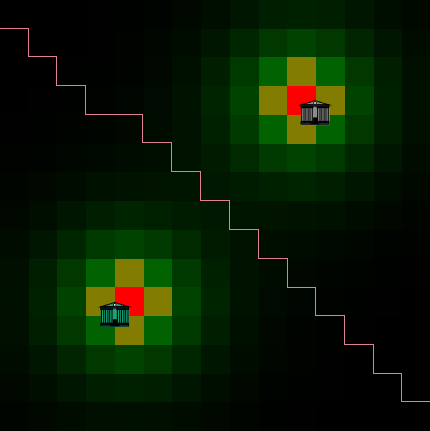
\includegraphics[width=0.49\linewidth]{Figures/Lutecia/ex_setup.png}
	%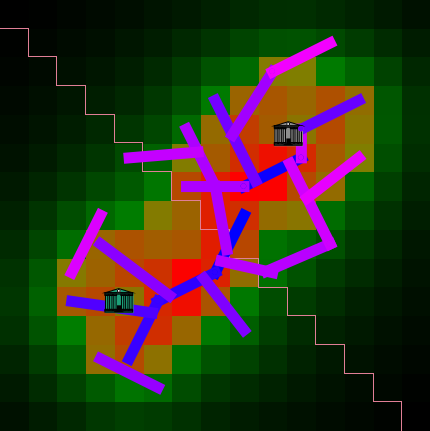
\includegraphics[width=0.49\linewidth]{Figures/Lutecia/ex_reg_infra50.png}
	%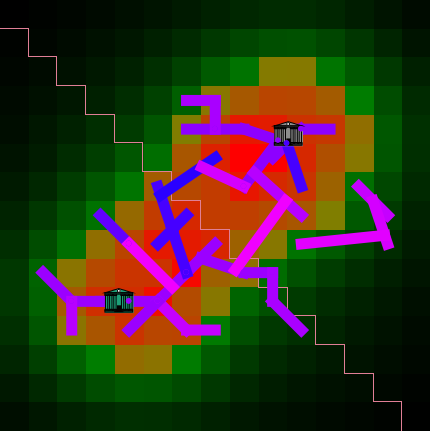
\includegraphics[width=0.49\linewidth]{Figures/Lutecia/ex_maxcollabcost_infra50.png}
	%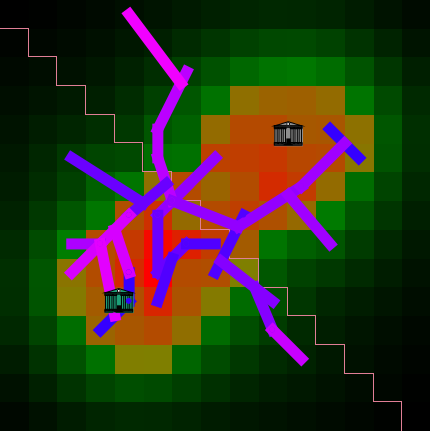
\includegraphics[width=0.49\linewidth]{Figures/Lutecia/ex_mincollabcost_infra50.png}
	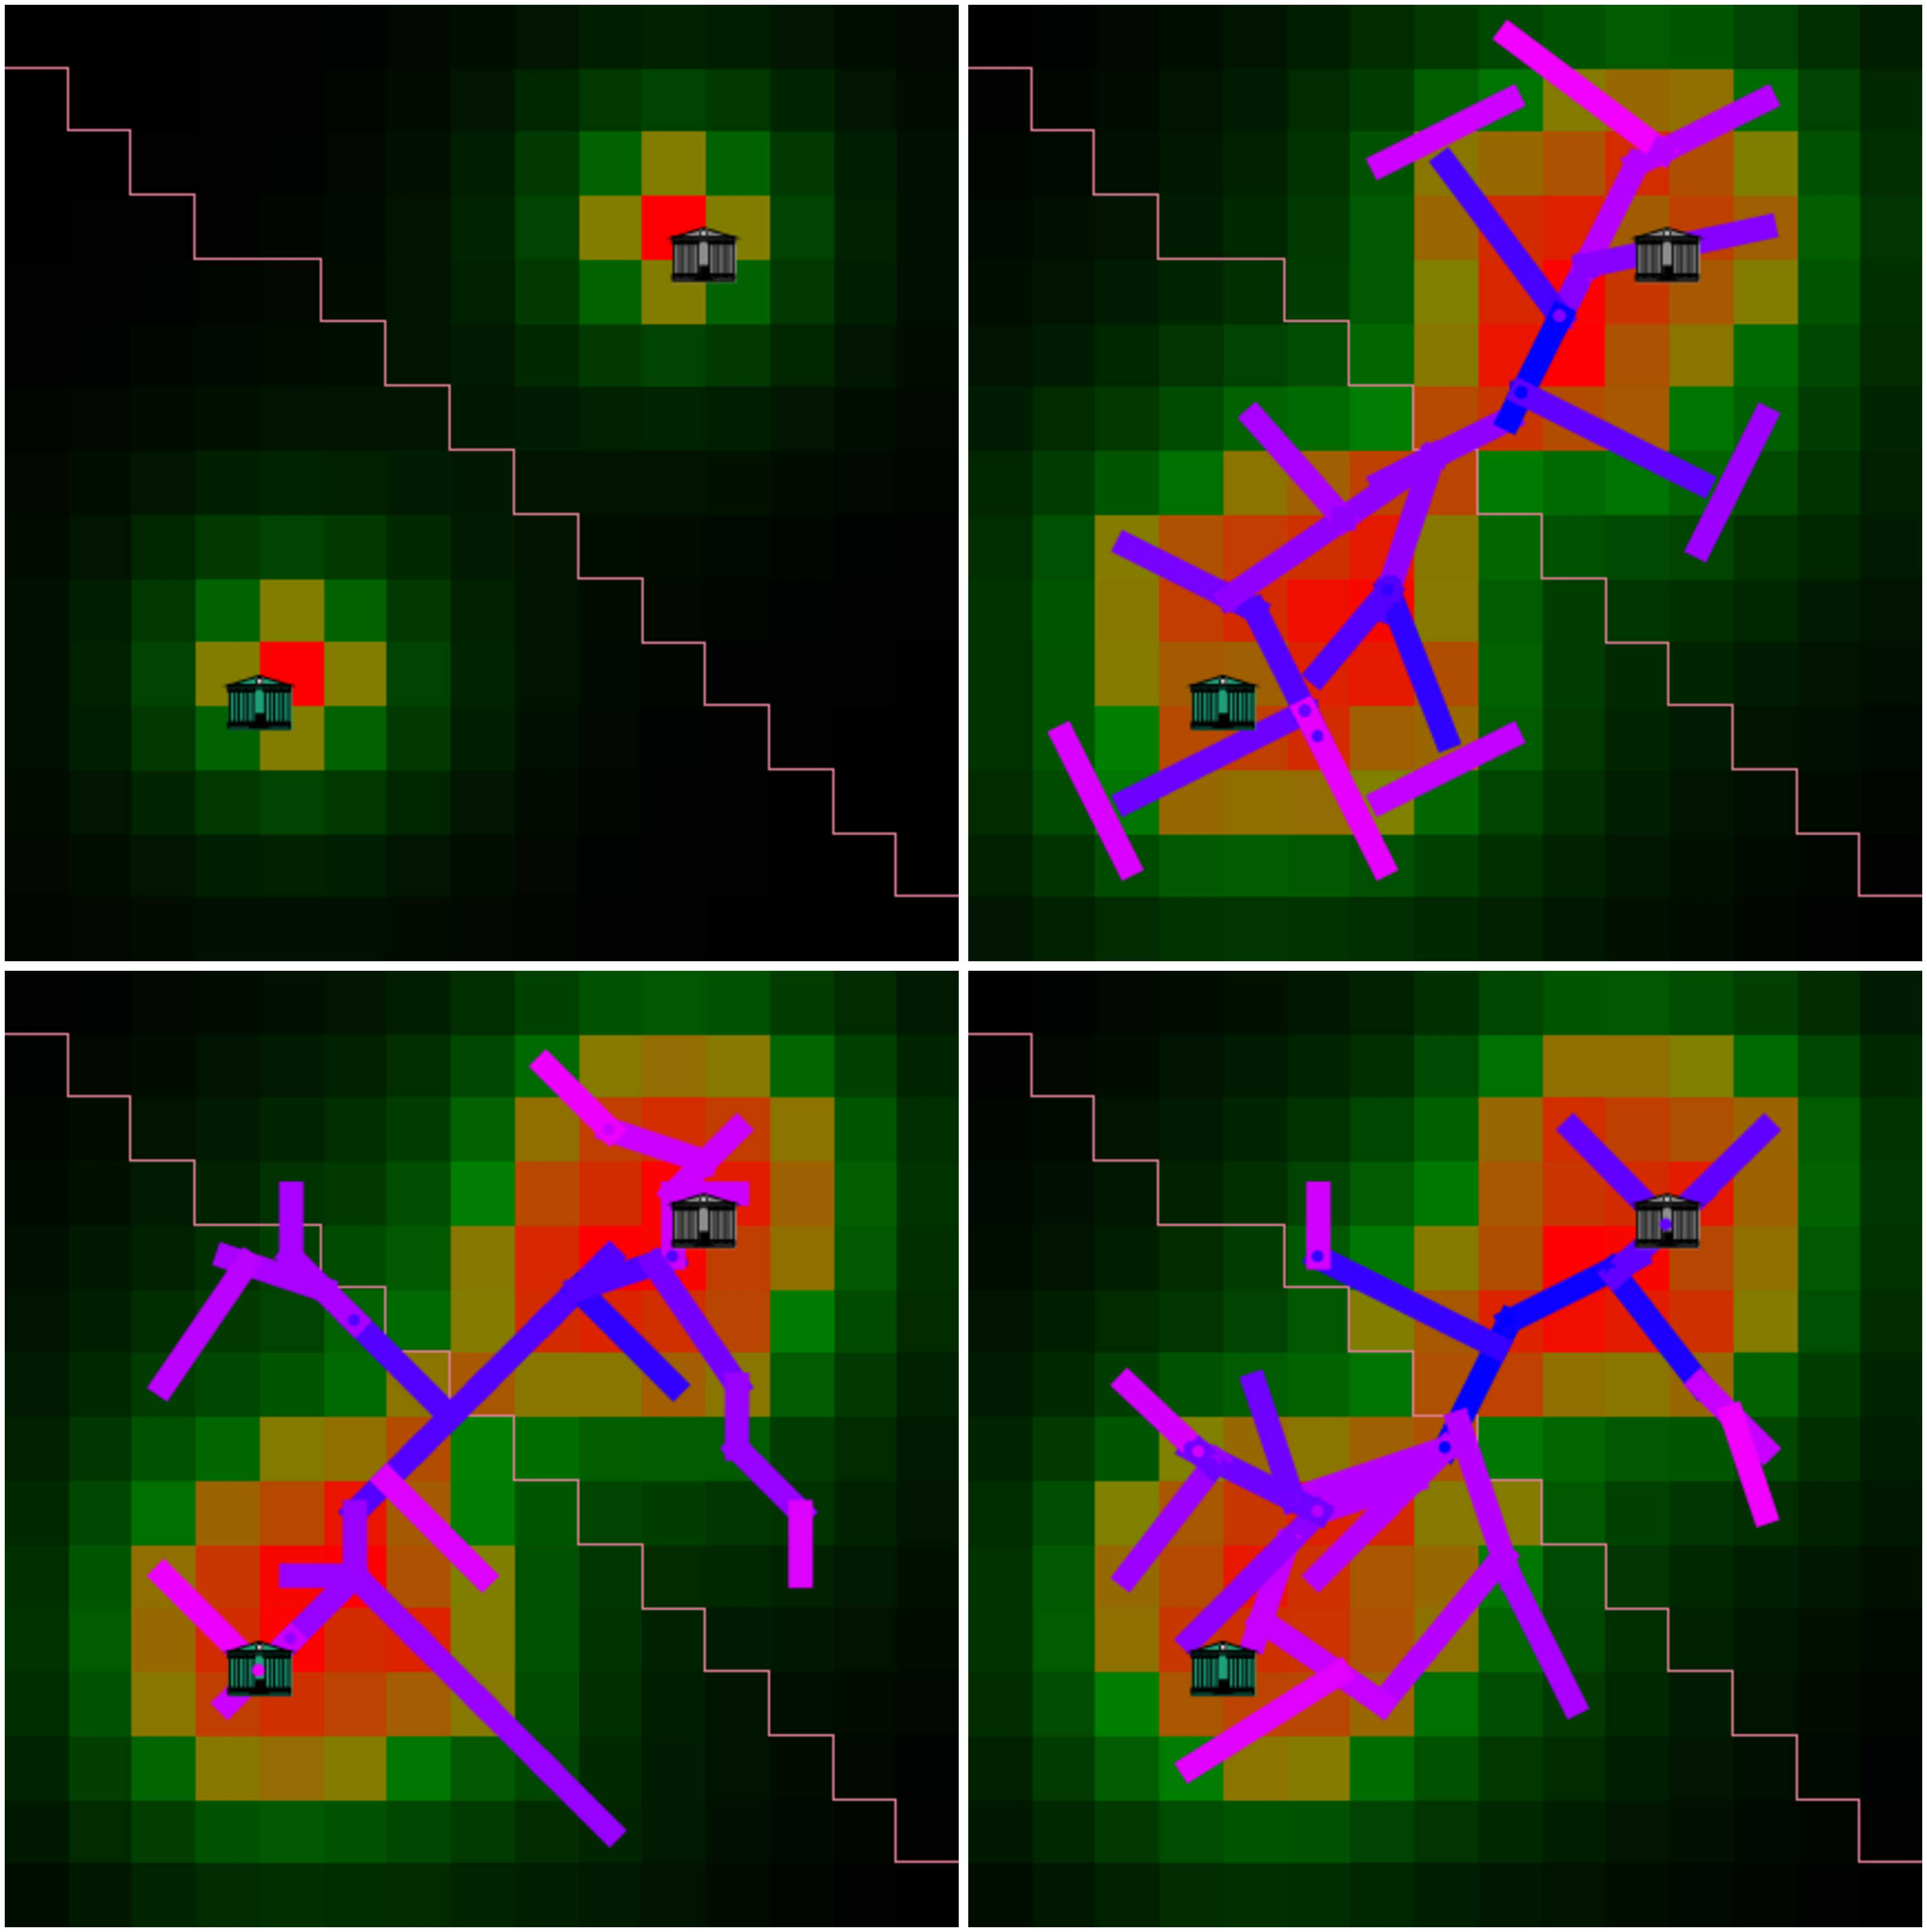
\includegraphics[width=\linewidth]{Figures/Final/7-3-3-fig-lutecia-governance.jpg}
	\caption[Network topologies obtained for different levels of governance][Formes de réseau obtenues pour différents niveaux de gouvernance]{\textbf{Network topologies obtained for different levels of governance.}\label{fig:lutecia:governance}}{\textbf{Formes de réseau obtenues pour différents niveaux de gouvernance.} Le modèle est initialisé sur une configuration synthétique symétrique à deux centres (\textit{Haut gauche}). Les paramètres pour l'évolution de l'usage du sol sont $\gamma_A = \gamma_E = 0.8 ; \beta = 2 ; \lambda = 0.001 ; \alpha = 0.16$, et pour l'évolution du réseau $l_r = 2$ et un jeu à choix discrets. L'évolution est stoppée à stock constant $S = 50$ et l'exploration heuristique faite pour $N_e = 200$. (\textit{Haut droite}) Niveau de décision régional ($\xi = 1$) ; (\textit{Bas gauche}) Niveau local ($\xi = 0$) et bas niveau de collaboration, obtenu avec un fort coût de coopération $J=0.005$ ; (\textit{Bas droite}) Niveau local et haut niveau de collaboration, avec $J=0$.\label{fig:lutecia:governance}}
\end{figure}
%%%%%%%%%%%%








%%%%%%%%%%%%%%%%%%%%
\subsection{Application to Pearl River Delta}{Application au Delta de la Rivière des Perles}


\bpar{
It was suggested by \cite{liao2017ouverture} that a sort of multi-level governance recently emerged in China, in the context of economic activities. We try with our model to test the relevance of this paradigm regarding the urban structure of the MCR.
}{
Il a été suggéré par \cite{liao2017ouverture} qu'une forme de gouvernance multi-niveau a récemment émergé en Chine, dans le contexte des activités économiques. Nous tentons par notre modèle de tester la pertinence de ce paradigme au regard de la structure urbaine de la MCR.
}






%
%
\subsubsection{Model setup}{Initialisation du modèle}

\bpar{
We work on a simplified raster configuration for population in Pearl River Delta, and on stylized highway networks. We choose to consider road network only since, following \cite{hou2011transport}, it has been the main driver of changes in accessibility patterns compared to railway network which development is only recent.
}{
Nous travaillons sur une configuration raster simplifiée (cellules de 5km) pour la population du Delta de la Rivière des Perles, ainsi que sur le réseau d'autoroute stylisé. Nous considérons le réseau routier uniquement puisque, selon \cite{hou2011transport}, il s'agit du moteur principal des changements dans les motifs d'accessibilité en comparaison au réseau ferré dont le développement accéléré est récent. Les réseaux sont stylisés à partir du plan donné par~\cite{hou2011transport} qui reproduit les documents officiels de la province du Guangdong en 2010. Nous considérons ainsi le réseau autoroutier en 2010 et celui planifié à cette époque. La Fig.~\ref{fig:lutecia:ex-prd} illustre la configuration stylisée pour le Delta de la Rivière des Perles.
}


%
%We show in Fig.~\ref{fig:ex-prd} an illustration of the stylized setup of the model and of its outcome with standard parameter values.


%%%%%%%%%%%%%%%%%%%%
\begin{figure}
%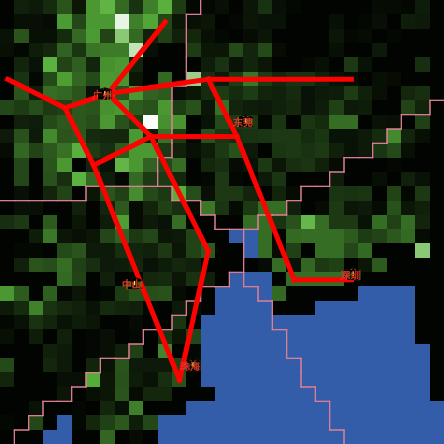
\includegraphics[width=0.49\linewidth]{Figures/Lutecia/exrun_2_tick0}
%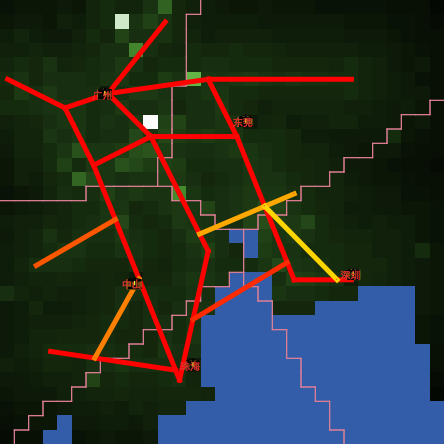
\includegraphics[width=0.49\linewidth]{Figures/Lutecia/exrun_2_tick6}
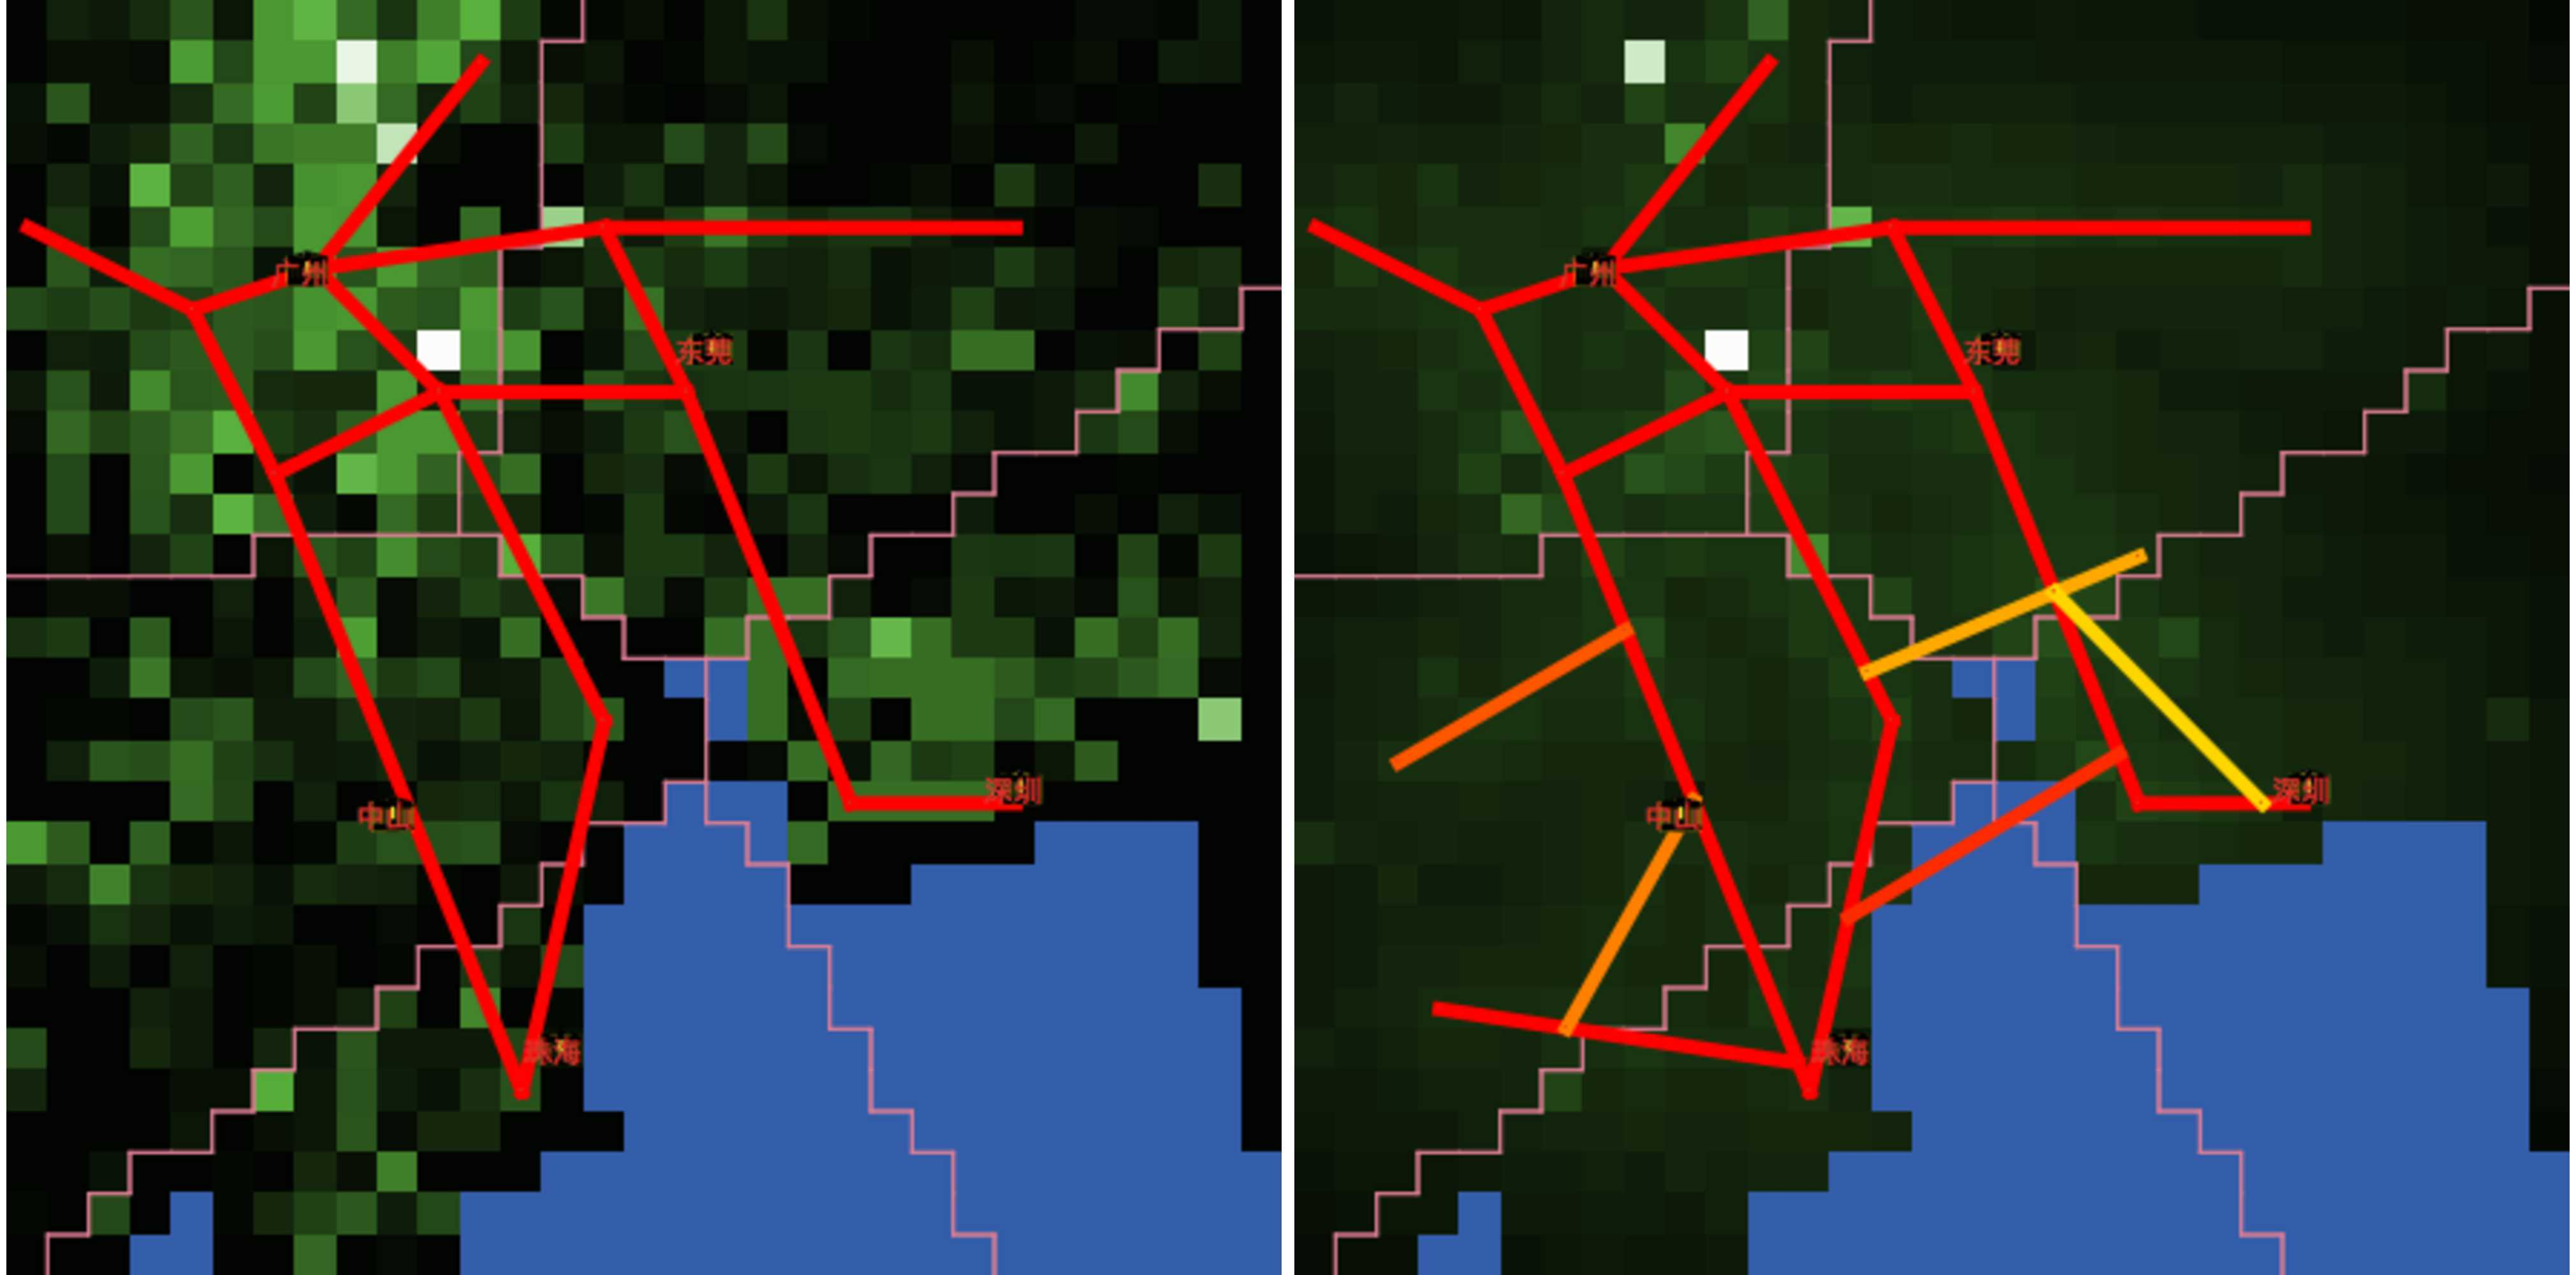
\includegraphics[width=\linewidth]{Figures/Final/7-3-3-fig-lutecia-ex-prd.jpg}
\caption[Application of Lutecia to PRD][Application de Lutecia au Delta de la Rivière des Perles]{\textbf{Example of run on the stylized Pearl River Delta.} (initial configuration and after 6 network iterations)\label{fig:lutecia:ex-prd}}{\textbf{Exemple d'application au Delta de la Rivière des Perles.} (\textit{Gauche}) Initialisation avec le raster de population 2010, agrégé à la résolution 5km, et le réseau autoroutier simplifié ; (\textit{Droite}) Etat après 6 pas de temps ($\alpha = 1$)\label{fig:lutecia:ex-prd}}
\end{figure}
%%%%%%%%%%%%%%%%%%%%





\subsubsection{Calibration procedure}{Procédure de calibration}


\bpar{
To apply such a complex model to a semi-real situation, one must be extremely careful. It is important to choose the adequate processes and level of granularity to reproduce. In particular, our model is not aimed at producing particularly accurate land-use patterns, but uses their approximation as the basis of network growth, which qualitative evolution and the corresponding qualitative patterns in governance processes. We propose therefore to ``calibrate'' on the shape of a given infrastructure, in the sense of determining parameter configurations for which in probability the successive built pieces of infrastructure are the closest to pieces of the target infrastructure. 
}{
Lors de l'application d'un modèle si complexe à une situation semi-réelle, il faut rester vigilant. Il est important de choisir les processus adéquats ainsi que le niveau de granularité à reproduire. En particulier, notre modèle produit des motifs d'usage du sol relativement précis, mais utilise leur approximation comme base de la croissance du réseau, dont l'évolution qualitative permet d'informer sur les processus de gouvernance. Nous proposons pour cela de ``calibrer'' sur la forme d'une infrastructure donnée, au sens de déterminer des configurations de paramètres pour lesquelles en probabilité les morceaux successifs d'infrastructure sont les plus proches d'une infrastructure visée.
}


\bpar{
To calibrate on the network produced by the simulation, it must be compared to a reference network. This is however a difficult problem, as different proximity measures with different significations can be used. Geometrical measures focuses on the spatial proximity of networks. For a network $(E,V)=((e_j),(v_i))$, a node-based distance is given by $\sum_{i \neq i'} d^2 \left(v_i,v_{i'}\right)$. A more accurate measure not biased by intermediate nodes is given by the cumulated area between each pair of edges $\sum_{j \neq j'} A \left(e_j,e_{j'}\right)$ (not a distance in the proper sense) where $A(e,e')$ is the area of the closed polygon formed by joining link extremities.
}{
Pour calibrer sur les réseaux produits par la simulation, il s'agit de comparer à un réseau de référence. C'est un problème difficile, puisque différentes mesures de proximité avec différentes signification peuvent être utilisées. Les mesures géométriques s'intéressent à la proximité spatiale des réseaux. Pour un réseau $(E,V)=((e_j),(v_i))$, une distance basée sur les noeuds est donnée par $\sum_{i \neq i'} d^2 \left(v_i,v_{i'}\right)$. Une mesure plus précise qui n'est pas biaisée par d'éventuels noeuds intermédiaires est donnée par l'aire cumulée entre chaque paire de liens $d_A = \sum_{j \neq j'} A \left(e_j,e_{j'}\right)$ (il ne s'agit pas d'une distance à proprement parler), où $A(e,e')$ est l'aire du polygone fermé constitué en reliant les sommets des liens. Nous considérerons cette dernière pour la calibration.
}




\subsubsection{Calibration}{Calibration}

Les expériences que nous menons sont à usage du sol fixé, le niveau de détail requis pour des données plus anciennes et plus récentes, voir des projections, pour la population et les emplois n'étant pas permis par les données à notre disposition.

Nous faisons varier les paramètres de gouvernance, incluant le type de jeu, avec $l_r = 2$ fixé, et explorons un échantillonnage LHS de 4000 points dans l'espace de ces paramètres, avec 10 répétitions du modèle pour chaque point. Les deux expériences menées correspondent à des configurations cible différentes :
\begin{itemize}
	\item pas de réseau initial et réseau de 2010 comme cible, dans l'esprit d'extrapoler la configuration de gouvernance la plus probable ayant mené à la configuration actuelle ;
	\item réseau 2010 initial, et réseau planifié comme cible : extrapolation de la configuration de gouvernance de la planification.
\end{itemize}

Nous obtenons des résultats qualitativement similaires pour les deux expériences, suggérant qu'il n'y a pas eu de transition de type de gouvernance entre réseau passé et réseau futur. Les résultats sont illustrés en Fig.~\ref{fig:lutecia:calib}. On obtient, à l'étude du graphe de $d_A$ en fonction de $\xi$, que le niveau régional est le plus fidèle pour reproduire la forme du réseau. Par contre, les jeux de choix discrets et de compétition se comporte différemment, et le jeu compétitif est le plus proche de la réalité quand $\xi$ diminue : les relations entre acteurs locaux seraient a priori de nature plus compétitive qu'égoïste. Quand on étudie la variation de la distance en fonction du niveau de collaboration observé, on obtient une forme intéressante en cloche inversée, c'est à dire que les situations les plus probables sont soit celles où il n'y a que de la collaboration, soit celles où il n'y en a pas du tout, mais pas de situations intermédiaires. Enfin, la comparaison des distributions statistiques des distances entre les configurations cibles et les types de jeux montre que la différence entre les jeux n'est considérable que pour le réseau réel mais pas le réseau planifié (conclusion difficile à interpréter).



%%%%%%%%%%%%%%%
\begin{figure}
	%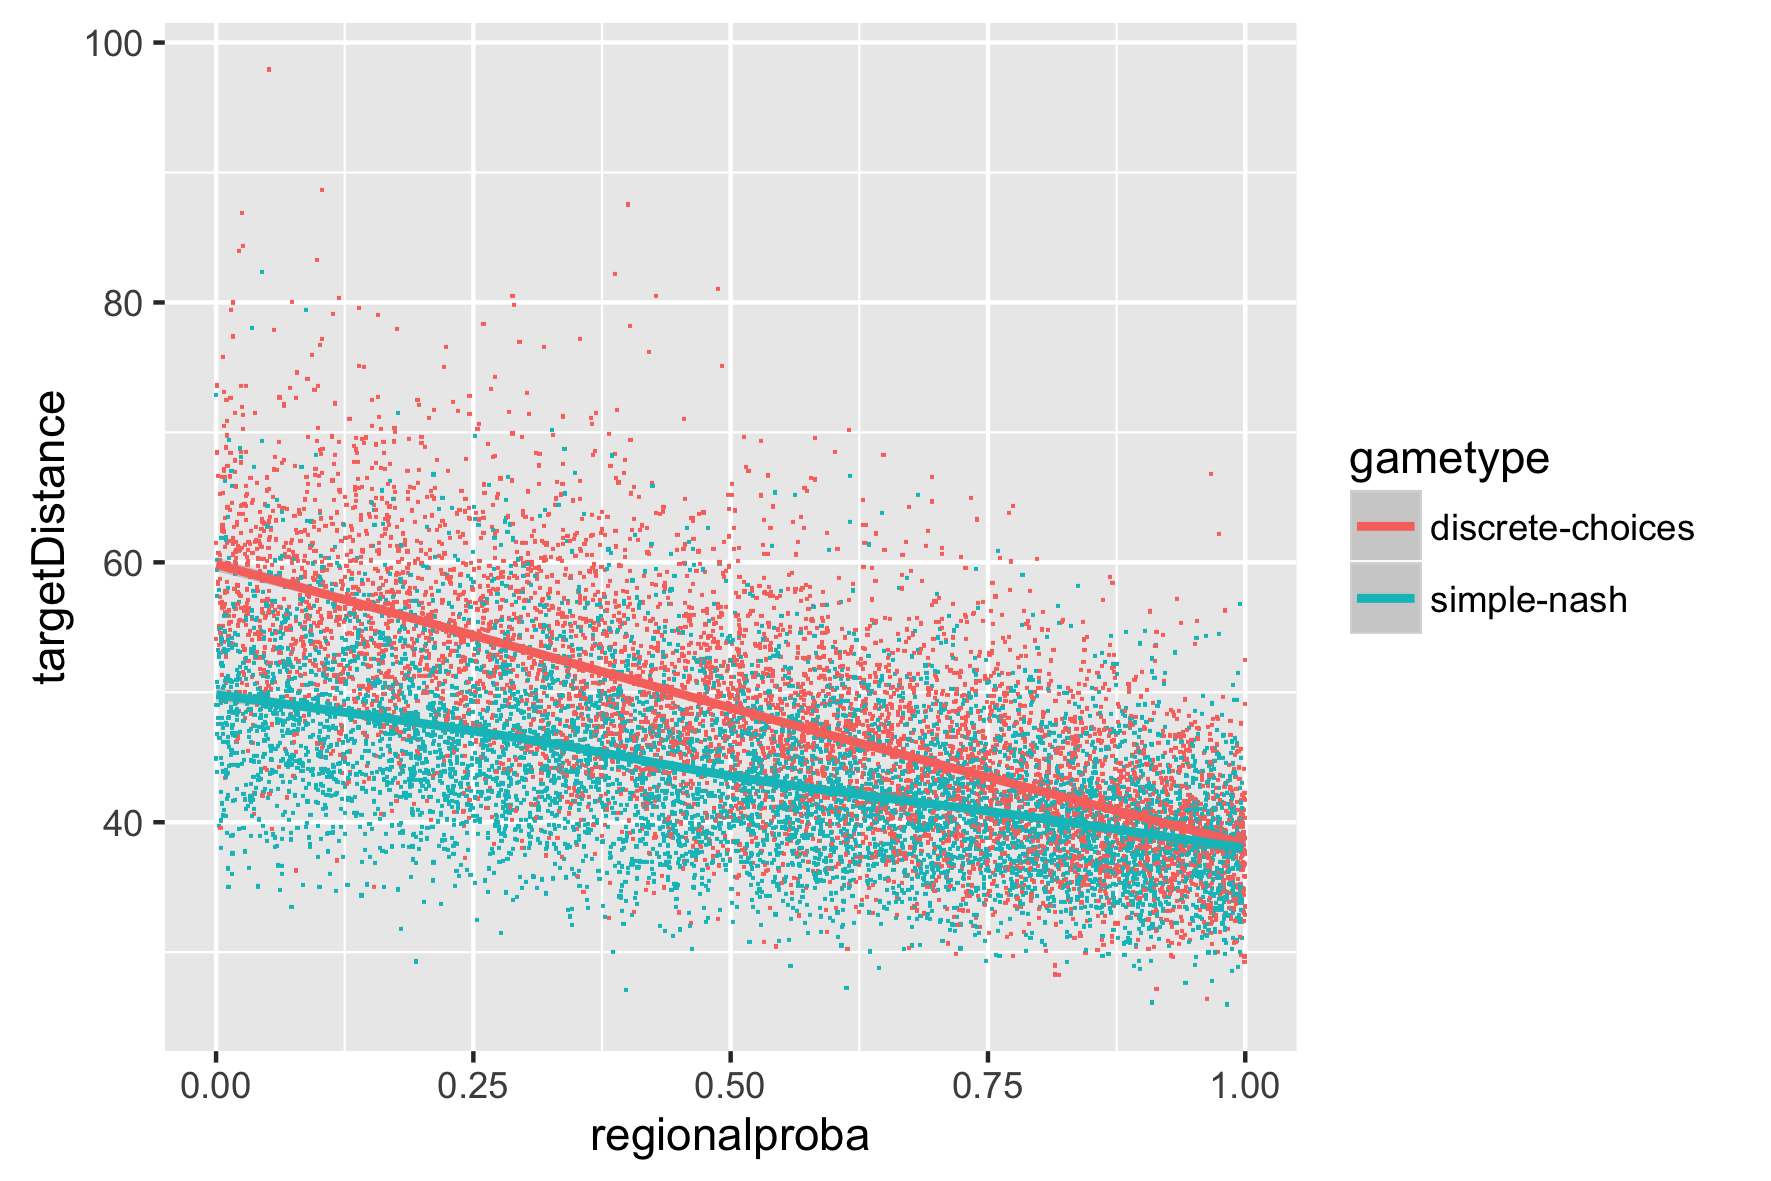
\includegraphics[width=0.49\linewidth]{Figures/Lutecia/regional-distance_colorgametype.png}
	%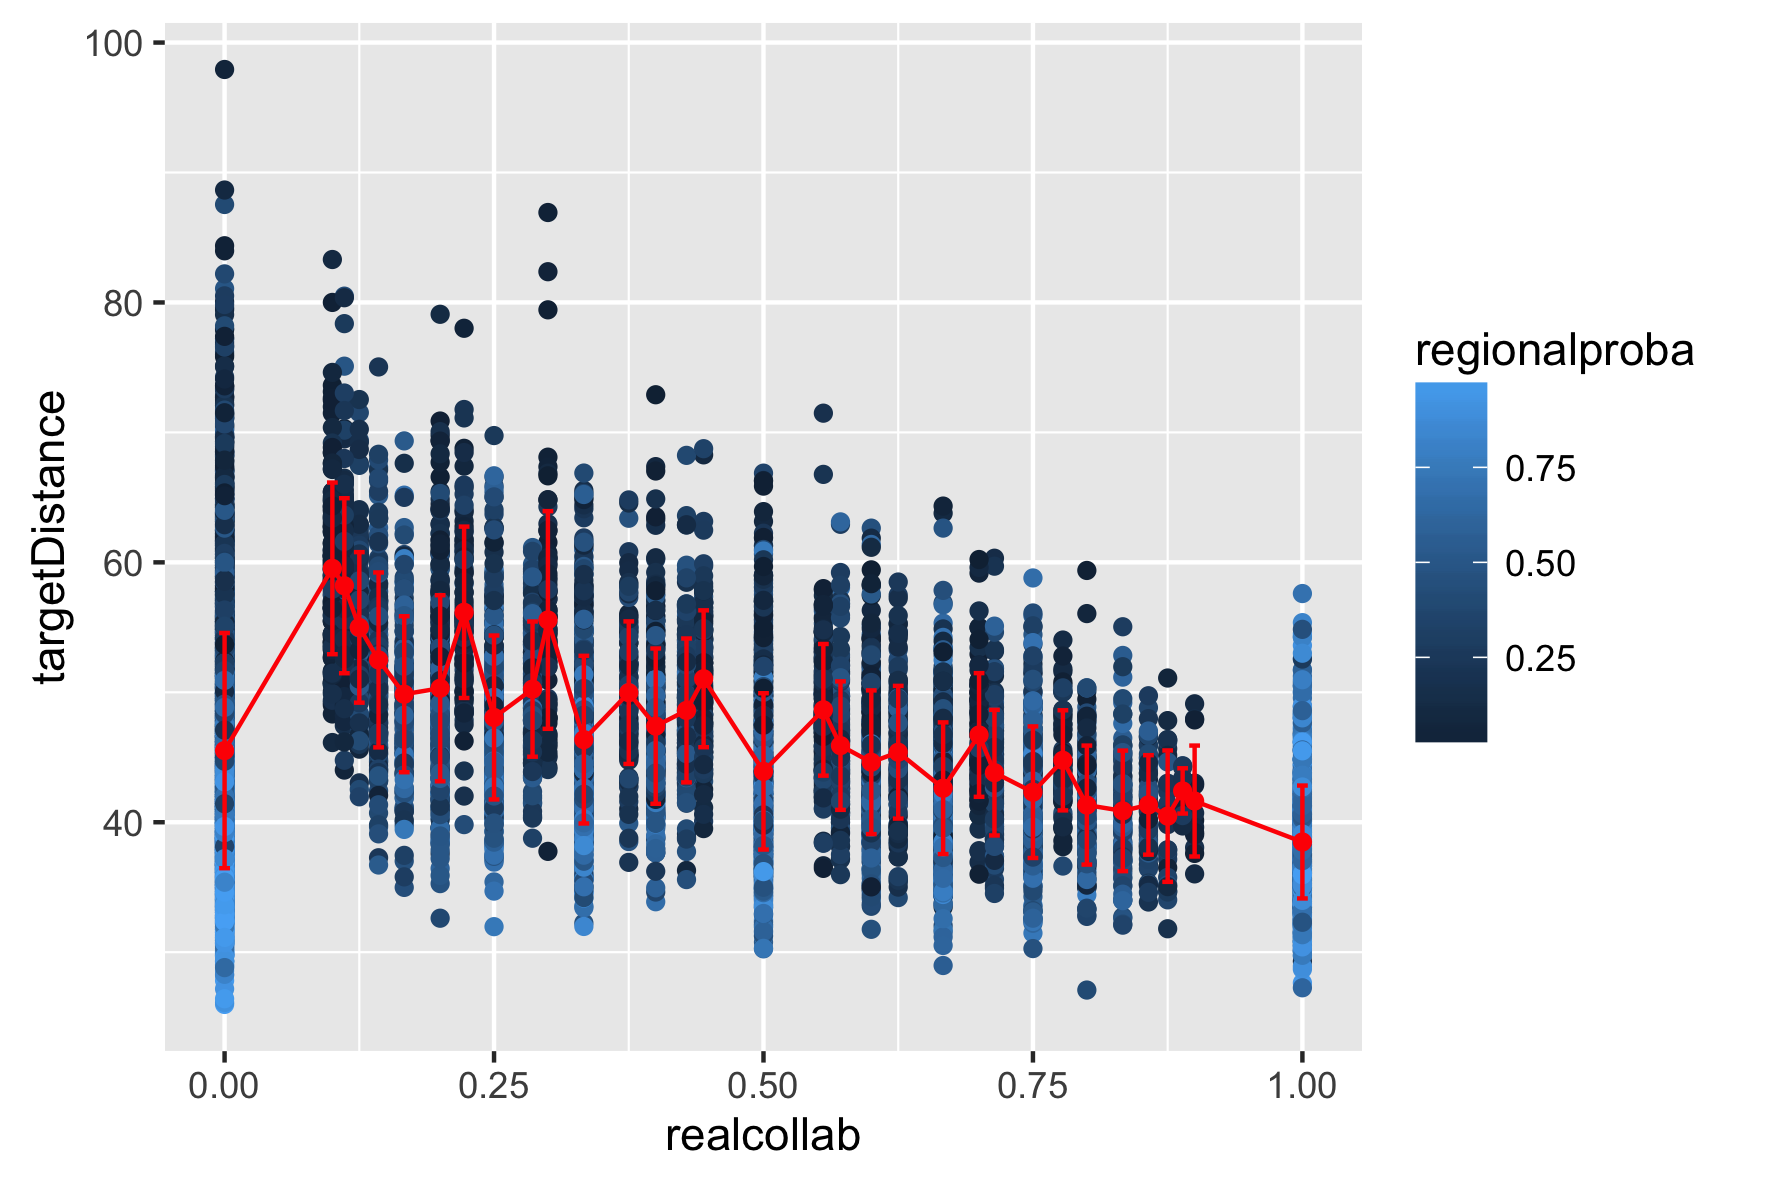
\includegraphics[width=0.49\linewidth]{Figures/Lutecia/collab-distance_colorregional.png}
	%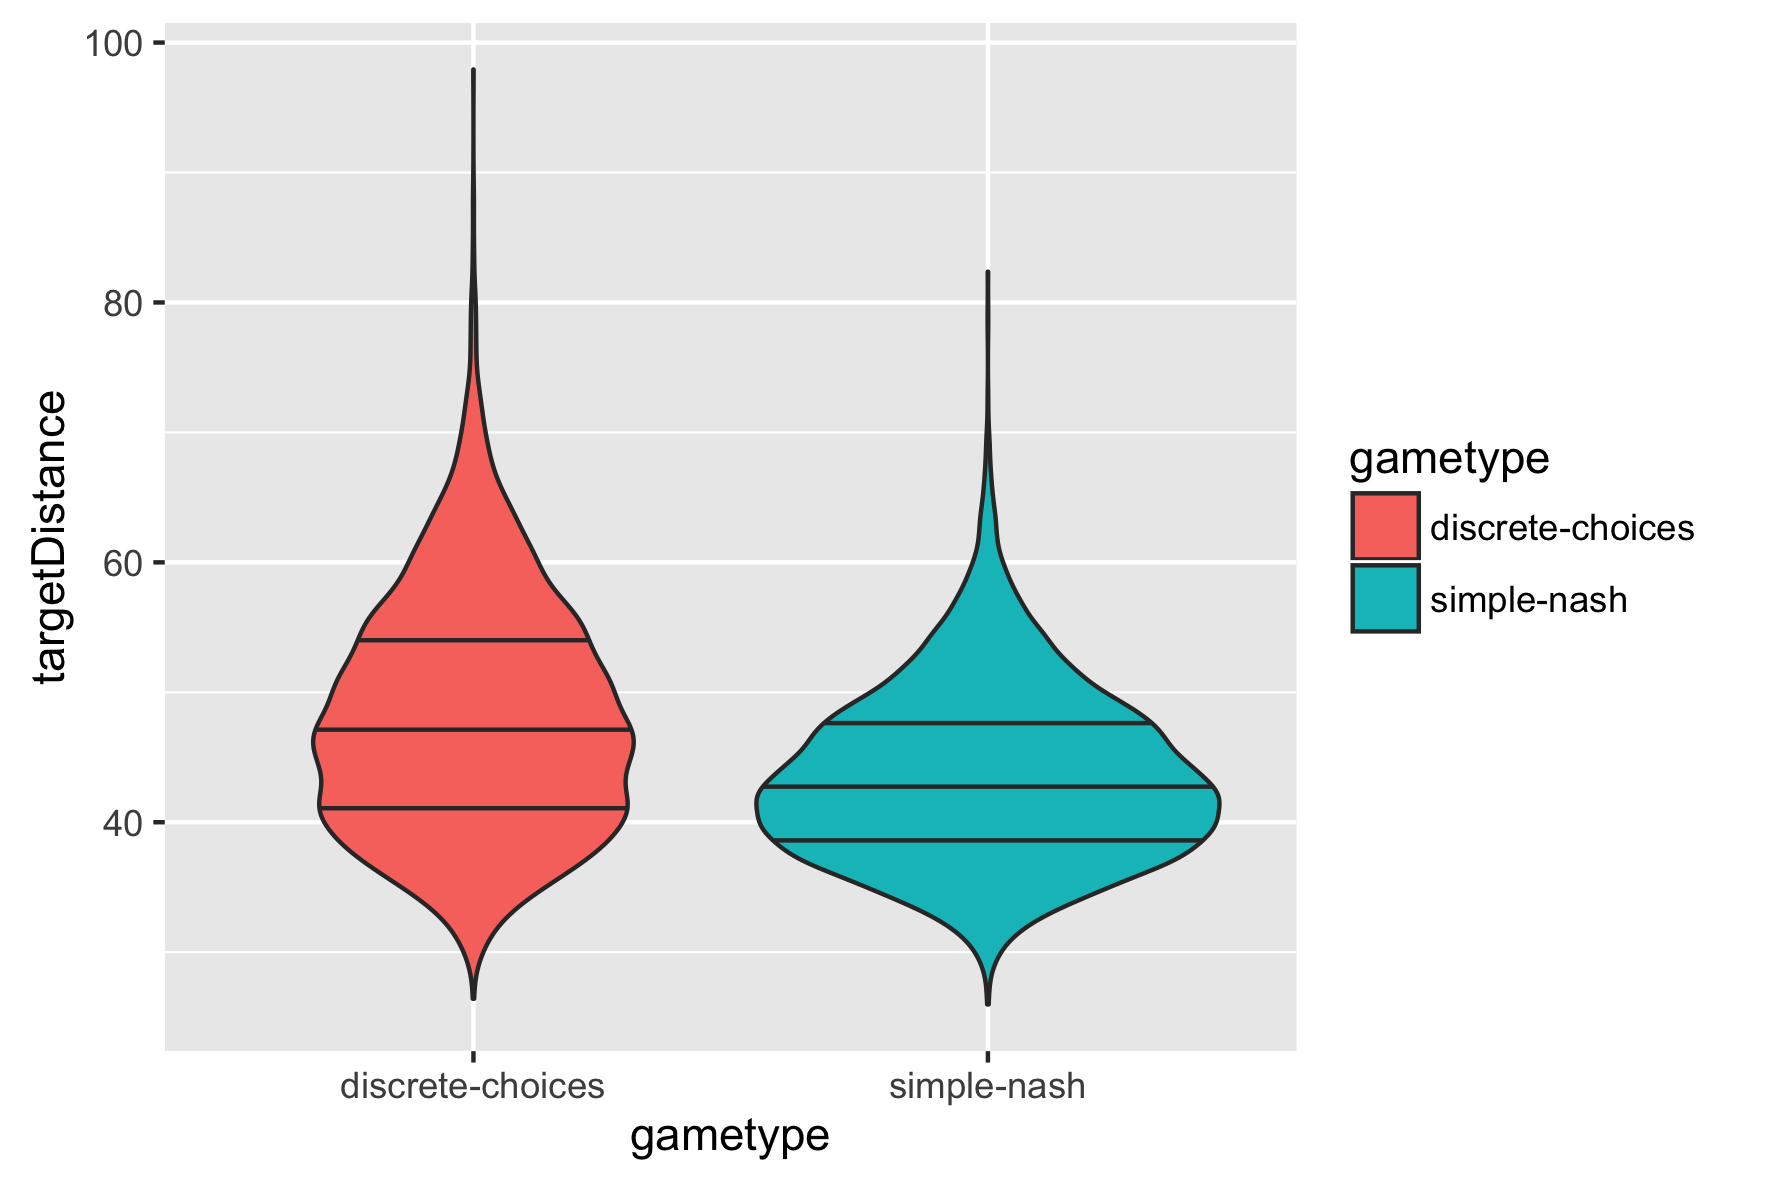
\includegraphics[width=0.49\linewidth]{Figures/Lutecia/distanceviolin_gametype.png}
	%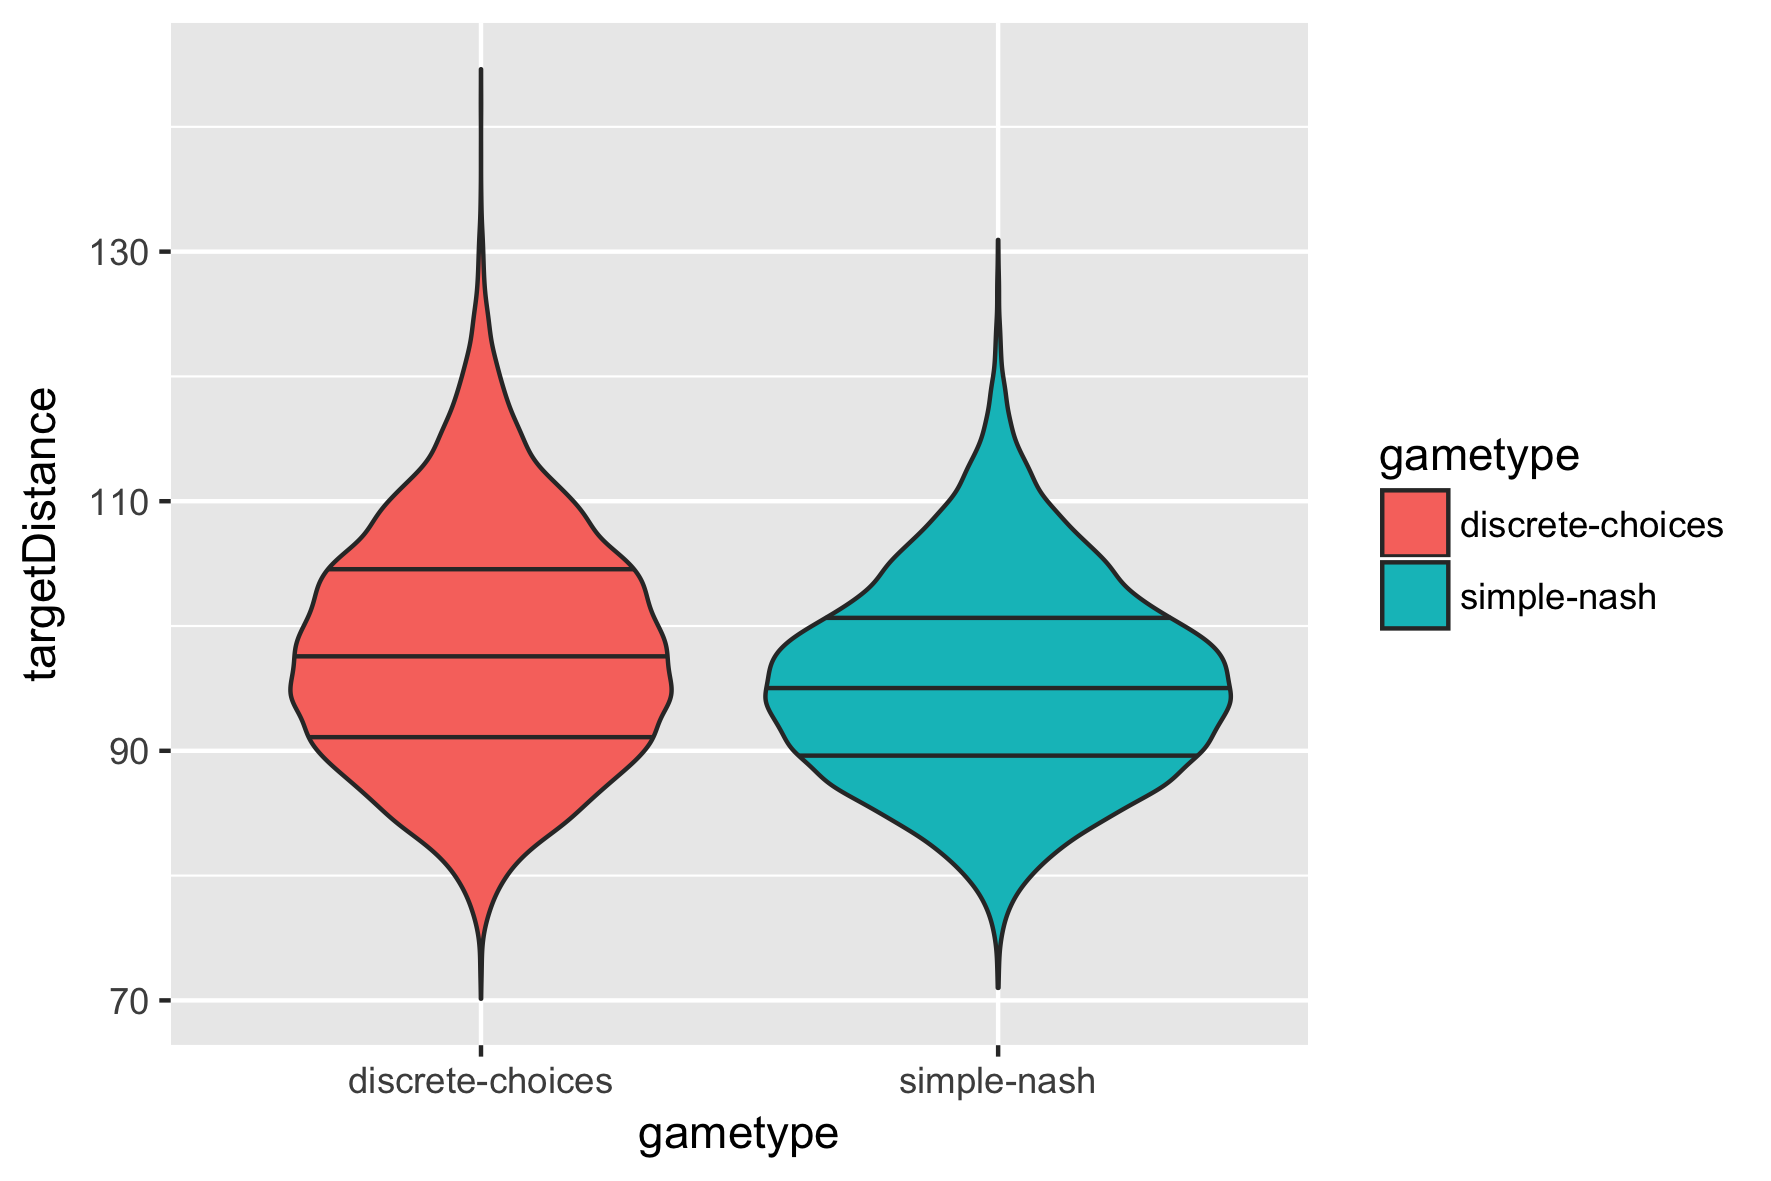
\includegraphics[width=0.49\linewidth]{Figures/Lutecia/distanceviolin_gametype_real.png}
	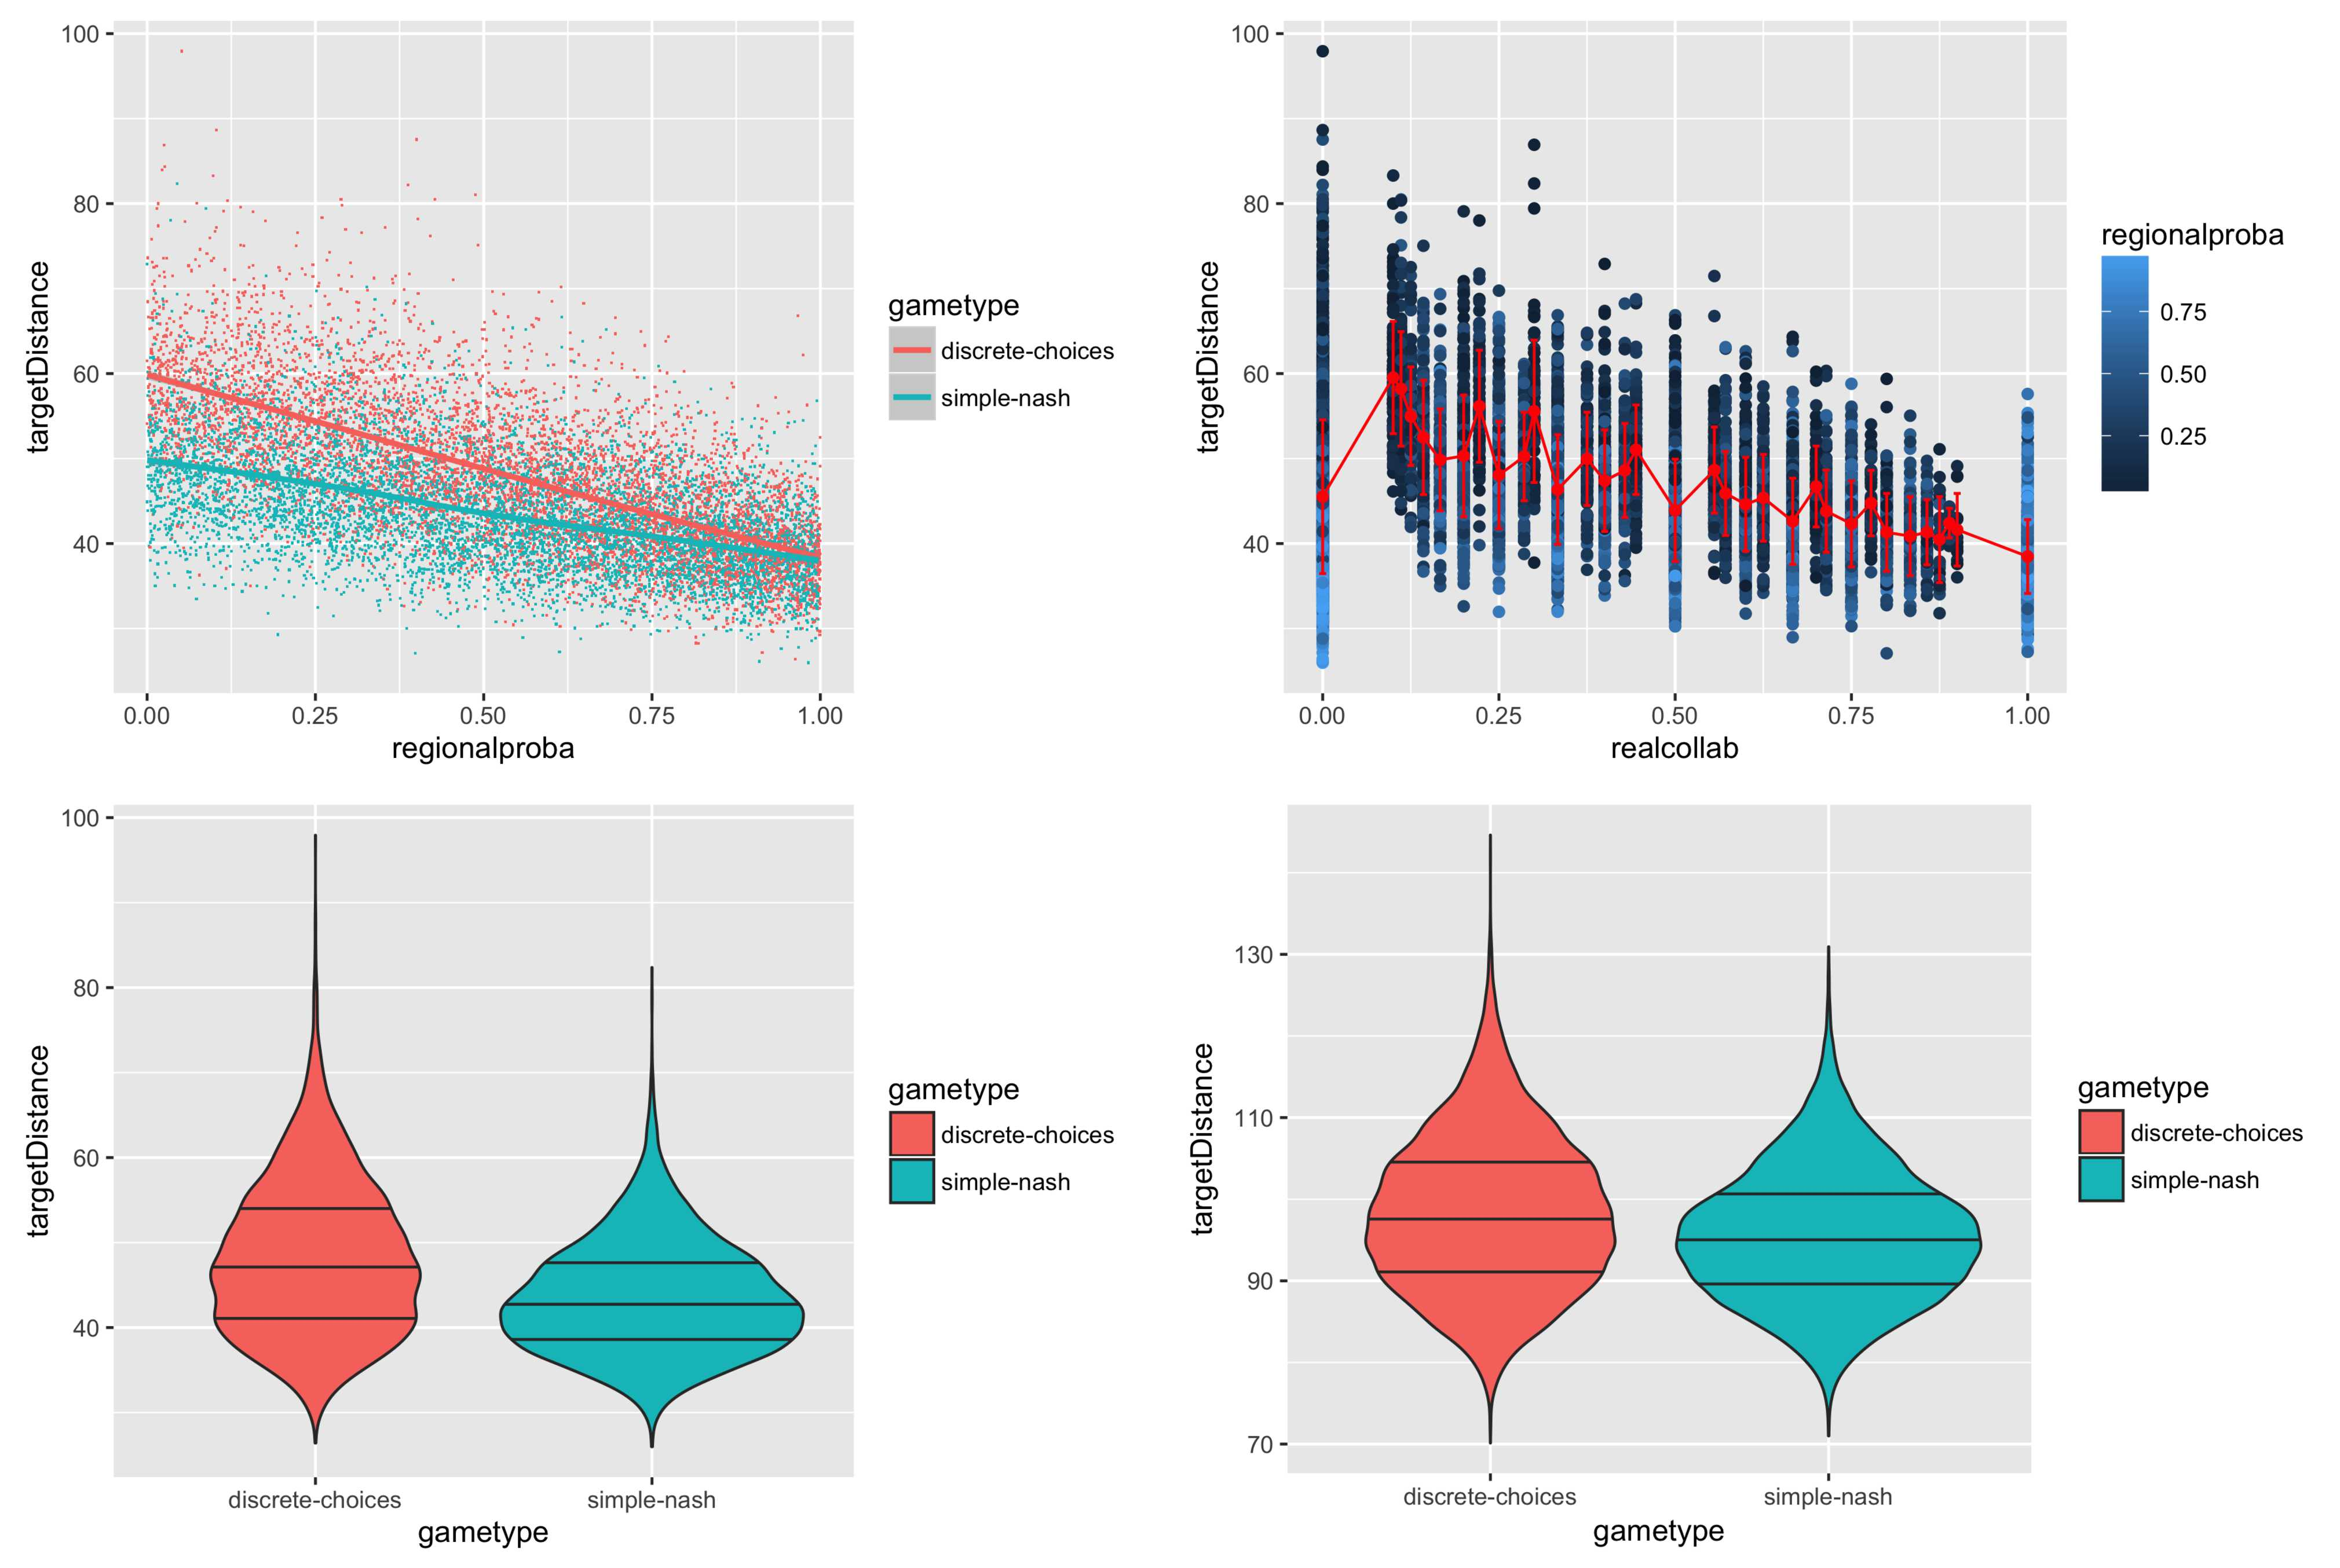
\includegraphics[width=\linewidth]{Figures/Final/7-3-3-fig-lutecia-calib.jpg}
	\caption[Calibration of the Lutecia model][Calibration du modèle Lutecia]{\textbf{Model calibration with fixed land use.}\label{fig:lutecia:calib}}{\textbf{Calibration du modèle à usage du sol fixé.} On prend $\alpha = 0$ pour ne faire évoluer que le réseau, et échantillonnons l'espace des paramètres de gouvernance. (\textit{Haut Gauche}) Distance $d_A$ au réseau cible (targetDistance), dans le cas du réseau réel, en fonction de la probabilité de décision régionale $\xi$ (regionalproba), pour les deux types de jeu (couleur). (\textit{Haut Droite}) Distance $d_A$ en fonction de la probabilité de collaboration observée (realcollab) ; la courbe rouge donne les moyennes avec les barres d'erreur. (\textit{Bas Gauche}) Distribution statistique de la distance en fonction du type de jeu, dans le cas du réseau réel ; (\textit{Bas Droite}) dans le cas du réseau planifié. \label{fig:lutecia:calib}}
\end{figure}
%%%%%%%%%%%%%%%



Nous tirons donc de cette expérience les conclusions suivantes, à prendre bien sûr avec prudence :
\begin{itemize}
	\item Une compétition entre les acteurs est plus probable qu'un comportement égoïste dans le cas de décisions locales.
	\item Les compromis de collaboration forment des réseaux moins probables que les situations avec pleine collaboration ou avec aucun collaboration.
\end{itemize}


Ces conclusions peuvent être mises en perspective avec la compétition accrue au sein du Delta révélée par~\cite{xu2005city}. Ainsi, cette application du modèle permet d'inférer indirectement des processus de gouvernance.  





\subsubsection{Discussion}{Discussion}

Bien que le modèle ait encore à être exploré plus en profondeur et pour l'ensemble de ses modules, certains développements possibles peuvent retenir notre attention.


\paragraph{Endogenous level of decision}{Niveau de décision endogène}


\bpar{
One interesting aspect to study would be the emergence of larger administrative zones, i.e. the emergence of new levels of governance in polycentric metropolitan areas. The reality is of course not as simple, as bottom-up initiatives such as collaboration between neighbor cities are interlaced with top-down decisions such as e.g. the ``M{\'e}tropole du Grand Paris'' which is a new administrative structure for Paris Area decided at the state level~\cite{gilli2009paris}. It would be however interesting to test conditions for emergence of governance patterns from the bottom-up in a conceptual way by extending the model and adding interactions and fusion between administrative entities.
}{
Une extension pertinente serait l'étude de l'émergence de zones administratives par agrégation, c'est à dire l'émergence de nouveaux niveaux de gouvernance dans une région métropolitaine polycentrique. L'exemple de la Métropole du Grand Paris en est une bonne illustration, puisqu'elle se situe entre les collectivités locales et la région ainsi que l'état~\cite{gilli2009paris}. Une extension du modèle avec des règles de fusion des entités est une direction potentielle pour étudier cette question.
}


\paragraph{Competition for an external ressource}{Compétition pour une ressource externe}


\bpar{
An interesting extension to the model would be to simulate the competition of territory for an external ressource (an airport for example). The rationale is to explore if different centers of the MCR will tend to cooperate or compete given an externality.
}{
L'influence des territoires extérieurs ou des externalités sur l'évolution d'une MCR est une question ouverte. Dans le cas d'une ressource commune, localisée dans l'emprise de la MCR, des dynamiques de compétition ou de collaboration peuvent s'instituer entre acteurs pour son exploitation. Ce modèle est une solution pour étudier cette situation de manière stylisée, et réaliser ainsi une expérience contrôlée sur les dynamiques de co-évolution, qui permettrait de répondre à des questions plus générales quant au rôle de l'isolation territoriale dans les processus de co-évolution.
}



Nous avons ainsi posé les premières briques de modèles visant à une intégration plus complexe des processus de co-évolution, en introduisant le modèle Lutetia qui a ensuite été validé de manière préliminaire et dont les potentialités ont été démontrée par l'application au cas d'étude du Delta de la Rivière des Perles.










\stars





%%%%%%%%%%%%%%%





%%%%%%%%%%%%%%%%%%%%%%%%%%%%%
% Chapter 9 : Opening
% Theoretical Framework




%----------------------------------------------------------------------------------------

\newpage

%\section[A Geographical Theory][Une Théorie Géographique]{A Geographical Theory for Networks and Territories}{Une Théorie Géographique des Territoires et des Réseaux}

\section{A geographical theory}{Une théorie géographique}

\label{sec:theory}

%----------------------------------------------------------------------------------------


%%%%%%%
%% -- Points restant à éclaircir --

% - \comment{(Florent)  peut être que des schémas pourraient aider le lecteur} pour la transition d'échelle morphogénétique notamment
% - \comment{(Florent) et y'a t'il des territorial niches ? par ailleurs pourquoi pas tester hypothèse niche mais pourquoi pas autre chose ?} -> a creuser selon résultats empiriques et de modélisation
% - sur morphogenese : \cite{desmarais1992premisses} ; \cite{levy2005formes}
% - \comment{(Arnaud) Notion de Niche}
%  - definition of scale and stationarity
%        \textit{Equivalence between existence of discrete scales and discrete stationarity levels ?}
%         // equivalence between space and time - ergodicité / non ergodicité
%  - Sur la demo stationarité locale : \comment{(Florent) on ne peut pas te suivre, on se demande si par ailleurs on doit le faire} ; \comment{(Florent) manque toute une discussion sur els objets géographiques, villes/systèmes de villes, etc. et les échelles de temps des dynamiques territoriales}
%    !!! Plus : !!! on suppose que la décomposition modulaire est fixe dans le temps, voir avec une décomposition variable ?
% \comment{(Florent) je ne comprends pas du tout sur quoi tu bâtis à ce stade. les objectifs, je pensais le fil, mais ou est la matière ? même si tu gardes cette approche très théorique, il faut que tu décomposes beaucoup plus}
% \comment{(Florent) a revoir, trop de choses sont non définies}
% \comment{(Arnaud) morphogenetic}
% 
% Network Necessity : \comment{(Florent) je ne suis pas convaincu qu'il y a beaucoup de faits stylisés absolument impossibles à reproduire sans réseaux. mais les inclure (les réseaux) a des avantages que tu vas défendre}
% 
% \comment{(Florent) parfait je pense que c'est une bonne idée. peux tu néanmoins le justifier dans le contexte actuel d'incertitude et de développement durable cela me semble pertinent.}
%
% Stationarité :  \comment{(Florent) peux tu expliquer pourquoi tu souhaites cette propriété ?}
% \comment{(Florent) je ne suis pas convaincu par cette distinction sur les échelles : c'est sans doute différent mais pas qualitativement}
%
% sur le réseau de neurones : \comment{(Florent) tu es dans la méthode c'est un autre point de discussion}




\bpar{
\noun{Raffestin} highlights in his preface of~\cite{offner1996reseaux} that a geographical theory that articulates spaces, networks and territories has never been formulated in a consistent way, since each approach has a vision reduced to some components only and does not aim at constructing an integrative theory. A research direction we propose to introduce here is the conjunction of approaches of the evolutive urban theory and of morphogenesis, to produce a theory that is both multi-scalar and fully integrates networks and territories.
}{
\noun{Raffestin} souligne dans sa préface de~\cite{offner1996reseaux} qu'une théorie géographique articulant espaces, réseaux et territoires n'a jamais été formulée de manière cohérente, chaque approche ayant une vision réduite à certaines composantes seulement et ne visant pas à construire une théorie intégrée. Une piste que nous proposons d'introduire ici est la conjonction des approches de la théorie évolutive des villes et de la morphogenèse, pour produire une théorie à la fois multi-scalaire et intégrant pleinement réseaux et territoires.
}




%%%%%%%%%%%
\subsection{Foundations}{Fondations}


\bpar{
Our theoretical construction relies on four pillars that we will detail below\footnote{Or more precisely a funding horizontal pillar which gives fundamental objects, i.e. foundations introduced in Chapter~\ref{ch:thematic}, two vertical pillars for the structure, and an horizontal synthesis pillar allowing to link these two.}.
}{
Notre construction théorique repose sur quatre piliers que nous détaillons ci-dessous\footnote{Ou plutôt un pilier horizontal de fondement qui précise les objets fondamentaux, c'est-à-dire les fondations introduites en Chapitre~\ref{ch:thematic}, deux piliers verticaux de structure, et un pilier horizontal de synthèse permettant de faire le lien entre ceux-ci.}.
}


%%%%%%%%%%%%%%
\subsubsection{Networked human territories}{Territoires humains en réseau}


\bpar{
Our first pillar corresponds to the theoretical construction elaborated in~\ref{sec:networkterritories}. We rely on the notion of \emph{Human Territory} elaborated by \noun{Raffestin} as the basis for a definition of a territorial system. It allows to capture complex human geographical systems in all the extent of their concrete and abstract characteristics, and also their representations. For example, a metropolitan territory can be apprehended simply by the functional extent of daily commuting flows, or by the perceived or lived space for different populations, the choice depending on the precise question that is considered.
}{
Notre premier pilier correspond à la construction théorique que nous avons élaborée en~\ref{sec:networkterritories}. Nous nous basons sur la notion de \emph{Territoire Humain} élaborée par \noun{Raffestin} comme la base de la définition d'un système territorial. Elle permet de capturer les systèmes complexes géographiques humains dans l'ensemble de leur caractéristiques concrètes et abstraites, ainsi que dans leur représentations. Par exemple, un territoire métropolitain peut être appréhendé simplement par l'étendue fonctionnelle des flux pendulaires journaliers, ou par l'espace perçu ou vécu des différentes populations, le choix dépendant de la question précise à laquelle on cherche à répondre.
}


\bpar{
The territory of \noun{Raffestin} indeed corresponds to a consistent system of \emph{synergetic inter-representation networks}, which are both a theory and a model for spatial cognition of individual and societies, constructed by \noun{Portugali} and \noun{Haken} (see~\cite{portugali2011sirn} for a synthetic presentation). It postulates that representations are the product of a strong coupling between individuals of cognitions and their individual and collective behaviors. This approach to the territory is of course a particular choice and other entries, possibly compatible, can be taken~\cite{murphy2012entente}.
}{
Le territoire de \noun{Raffestin} correspond en fait à un système cohérent de réseaux synergétiques d'inter-représentations (\emph{synergetic inter-representation networks}), qui sont à la fois une théorie et un modèle pour la cognition spatiale des individus et des sociétés, construite par \noun{Portugali} et \noun{Haken} (voir~\cite{portugali2011sirn} pour une présentation synthétique). Elle postule que les représentations sont le produit du couplage fort entre les individus des cognitions et de leurs comportements individuels et collectifs. Cette approche au territoire est bien sûr un choix particulier et d'autres entrées, possiblement compatibles, peuvent être prises~\cite{murphy2012entente}.
}

\bpar{
The concrete of this pillar in reinforced by the territorial theory of networks of \noun{Dupuy}, yielding the notion of networked human territory, as a human territory in which a set of potential transactional networks have been realized, which is in accordance with visions of the territory as networked places~\cite{champollion:halshs-00999026}. We will not use the implications of the development of the notion of \emph{place}, these being too sparse (see the definition of \cite{hypergeo}), and because of the redundancy with the territory in the vision of a complex link between representations and the physical reality. We will assume for this first pillar the fundamental assumption, already introduced in Chapter~\ref{ch:thematic}, that real networks are necessary ele;ents of territorial systems.
}{
Le ciment de ce pilier est renforcé par la théorie territoriale des réseaux de \noun{Dupuy}, fournissant la notion de territoire humain en réseau, comme un territoire humain dans lequel un ensemble de réseaux transactionnels potentiels ont été réalisés, ce qui s'accorde par ailleurs avec les visions du territoire comme un lieu des réseaux~\cite{champollion:halshs-00999026}. Nous n'utiliserons pas les implications du développement de la notion de \emph{lieu}, celles-ci étant trop éparses (voir définition de \cite{hypergeo}), et à cause de la redondance avec le territoire dans la vision de lien complexe entre représentation et réalité physique. Nous ferons pour ce premier pilier l'hypothèse fondamentale, déjà introduite en Chapitre~\ref{ch:thematic}, que les réseaux réels sont des éléments nécessaires des systèmes territoriaux.
}

% beware confusion between place and space : lieu en réseau ≠ lieu des réseaux ≠ espace en réseau ≠ espace des réseaux ???


%%%%%%%%%%%%%%%
\subsubsection{Evolutive urban theory}{Théorie évolutive des villes}



\bpar{
The second pillar of our theoretical construction is \noun{Pumain}'s evolutive urban theory, in close relation with the complex approach that we generally take. It has already been presented with details and its implications have been explored in Chapter~\ref{ch:evolutiveurban}. Here, this theory allows us to interpret territorial systems as complex adaptive systems and to introduce the co-evolution.
}{
Le second pilier de notre construction théorique est la théorie évolutive des villes de \noun{Pumain}, en relation étroite avec l'approche complexe que nous prenons de manière générale. Celle-ci a déjà été présenté en détails et ses implications ont été explorées en Chapitre~\ref{ch:evolutiveurban}. Ici, cette théorie nous permet d'interpréter les systèmes territoriaux comme systèmes complexes adaptatifs et d'introduire la co-évolution.
}





%%%%%%%%%%%
\subsubsection{Urban morphogenesis}{Morphogenèse Urbaine}

% -> make a link between city systems and urban form/cityscape / territorial configurations

% Why morphogenesis is important : linked with modularity and scale -> if a submodule can be explained independantly (ie morphigeneis process is isolated), then we have the characteristic scale. then when size grows and interaction within city system -> can not explain alone (or with externalities ?) -> need a change in scale. ex. influecne of city system for size, activities; posiiton of an airport in a metropoltian region ; emergence of MCR.  ==> Assimptions to be tested with models ?.

% Alexander and Salingaros

% include transportation network, hierarchy and congestion in transport : Remy vs Benjamin (paper ? -> see with René)



\bpar{
The notion of morphogenesis has been deeply explored and with an interdisciplinary point of view in~\ref{sec:interdiscmorphogenesis}. We recall here important axis and to what extent these contribute to the construction of our theory. Morphogenesis has been formalized especially by~\cite{turing1952chemical} which proposes to isolate elementary chemical rules that could lead to the emergence of the embryo and its form.
}{
Le concept de morphogenèse a été déjà exploré en profondeur et selon un point de vue interdisciplinaire en~\ref{sec:interdiscmorphogenesis}. Nous rappelons ici certains grands axes et dans quelle mesure ceux-ci contribuent à la construction de notre théorie. La morphogenèse a été formalisée notamment par~\cite{turing1952chemical} qui propose d'isoler des règles chimiques élémentaires qui pourraient mener à l'émergence de l'embryon et à sa forme.
}


\bpar{
The morphogenesis of a system consists in evolution rules that produce the emergence of its successives states, i.e. the precise definition of self-organization, with the additional property that an emergent architecture exists, in the sense of causal circular relations between the form and the function. Progresses towards the understanding of embryo morphogenesis (in particular the isolation of particular processes producing the differentiation of cells from an unique cell) have been made only recently with the use of complexity approaches in integrative biology~\cite{delile2016chapitre}.
}{
La morphogenèse d'un système consiste en des règles d'évolution qui produisent l'émergence de ses états successifs, i.e. la définition précise de l'auto-organisation, avec la propriété supplémentaire qu'une architecture émergente existe, au sens de relations causales circulaires entre la forme et la fonction. Les progrès vers la compréhension de la morphogenèse de l'embryon (en particulier l'isolation de processus particuliers induisant la différentiation de cellules à partir d'une unique) sont relativement récents grâce à l'application des approches complexes en biologie intégrative~\cite{delile2016chapitre}.
}


\bpar{
In the case of urban systems, the idea of urban morphogenesis, i.e. of self-consistent mechanisms that would produce the urban form, is more used in the field of architecture and urban design (as for example the generative grammar of ``Pattern Language'' of \cite{alexander1977pattern}), in relation with theories of urban form~\cite{moudon1997urban}. This idea can be pushed into very large scales such as the one of the building~\cite{whitehand1999urban} but we will use it more at a mesoscopic scale, in terms of land-use changes within an intermediate scale of territorial systems, with similar ontologies as the urban morphogenesis modeling literature (for example \cite{bonin2012modele} describes a model of urban morphogenesis with qualitative differentiation, whereas \cite{makse1998modeling} give a model of urban growth based on a mono-centric population distribution perturbed with correlated noises).
}{
Dans le cas des systèmes urbains, l'idée de morphogenèse urbaine, i.e. de mécanismes auto-cohérents qui produiraient la forme urbaine, est plutôt utilisé dans les champs de l'architecture et de l'urbanisme (comme par exemple la grammaire générative du ``Pattern Language'' de \cite{alexander1977pattern}), en relation avec des théories de la forme urbaine~\cite{moudon1997urban}. Cette idée peut être poussée jusqu'à de très grandes échelles comme celle du bâtiment~\cite{whitehand1999urban} mais nous la considérons à une échelle mesoscopique, en termes de changements d'usage du sol à une échelle intermédiaire des systèmes territoriaux, avec des ontologies similaires à la littérature de modélisation de la morphogenèse urbaine (par exemple \cite{bonin2012modele} décrit un modèle de morphogenèse urbaine avec différentiation qualitative, tandis que \cite{makse1998modeling} donne un modèle de croissance urbaine basé sur une distribution monocentrique de la population perturbée par des bruits corrélés).
}


\bpar{
The concept of morphogenesis is important in our theory in link with modularity and scale. Modularity of a complex system consists in its decomposition into relatively independent sub-modules, and the modular decomposition of a system can be seen as a way to disentangle non-intrinsic correlations~\cite{2015arXiv150904386K} (to have an idea, think of a block diagonalisation of a first order dynamical system). In the context of large-scale cyber-physical systems design and control, similar issues naturally raise and specific techniques are needed to scale up simple control methods~\cite{2017arXiv170105880W}. The isolation of a subsystem yields a corresponding characteristic scale. Isolating possible morphogenesis processes implies a controlled extraction (controlled boundary conditions e.g.) of the considered system, corresponding to a modularity level and thus a scale.
}{
Le concept de morphogenèse est important dans notre théorie en lien avec la modularité et l'échelle. La modularité d'un système complexe consiste en sa décomposition en sous-modules relativement indépendants, et la décomposition modulaire d'un système peut être vue comme un moyen de supprimer les corrélations non intrinsèques \cite{2015arXiv150904386K} (pour donner une image, penser à une diagonalisation par blocs d'un système dynamique du premier ordre). Dans le cadre de la conception et du contrôle de systèmes cyber-sociaux à grande échelle, des problèmes similaires surgissent naturellement et des techniques spécifiques sont nécessaires pour le passage à l'échelle des techniques simple de contrôle \cite{2017arXiv170105880W}. L'isolation d'un sous-système fournit une échelle caractéristique correspondante. Isoler des processus de morphogenèse possibles implique une extraction contrôlée (conditions au bord contrôlées par exemple) du système considéré, ce qui correspond à un niveau de modularité et donc à une échelle.
}

\bpar{
When local processes are not enough to explain the evolution of a system (with reasonable variations of initial conditions), a change of scale is necessary, caused by an underlying phase transition in modularity. The example of metropolitan growth is a good example: complexity of interactions within the metropolitan region will grow with size and the diversity of functions, leading to a change in the scale necessary to understand processes. The characteristic scales and the nature of processes for which these change occur can be precise questions investigated through modeling.
}{
Quand des processus locaux ne sont pas suffisants pour expliquer l'évolution d'un système (dans des variations raisonnables des conditions initiales), un changement d'échelle est nécessaire, causé par une transition de phase implicite dans la modularité. L'exemple de la croissance métropolitaine en est une très bonne illustration : la complexité des interactions au sein de la région métropolitaine sera croissante avec sa taille et la diversité des fonctions urbaines, ce qui conduit à un changement de l'échelle nécessaire pour comprendre les processus. Les échelles caractéristiques et la nature des processus pour lesquels ces changements ont lieu peuvent être des questions précisément approchées par l'angle de la modélisation.
}

% L'émergence d'un aéroport international pourra dans certains cas influencer fortement le développement local, ce qui correspondra à une intégration significative dans un système plus vaste.


\bpar{
Finally, it is important to remark as we did in~\ref{sec:interdiscmorphogenesis} that a territorial subsystem for which morphogenesis makes sense, which boundaries are well defined and which processes allow it to maintain itself as a network of processes, is close to an \emph{auto-poietic system} in the extended sense of \noun{Bourgine} in~\cite{bourgine2004autopoiesis}\footnote{Which are however not cognitive, making these morphogenetic systems not alive in the sense of auto-poietic and cognitive. Given the difficulty to define the delineation of cities for example, we will leave open the issue of the existence of auto-poietic territorial systems, and will consider in the following a less restrictive point of view on boundaries.}. These systems regulate then their boundary conditions, what underlines the importance of boundaries that we will finally develop.
}{
Enfin, il est important de noter comme nous l'avons fait en~\ref{sec:interdiscmorphogenesis} qu'un sous-système territorial pour lequel la morphogenèse prend sens, dont les frontières sont bien définies et dont les processus lui permettent de se maintenir en tant que réseau de processus, est proche d'un \emph{système auto-poiétique} au sens étendu de \noun{Bourgine} dans~\cite{bourgine2004autopoiesis}\footnote{Qui ne sont toutefois pas cognitifs, ne rendant pas ces systèmes morphogénétiques vivants au sens de auto-poiétique et cognitif. Vu la difficulté de définir la délimitation des villes par exemple, nous laisserons ouverte la question de l'existence de systèmes territoriaux auto-poiétiques, et considérerons par la suite un point de vue moins restrictif sur les frontières.}. Ces systèmes régulent alors leur conditions aux bords, ce qui souligne l'importance des frontières sur lesquelles nous allons finalement nous attarder.
}



%%%%%%%%%%%
\subsubsection{Co-evolution}{Co-évolution}

% other insight : Holland Signal and Boundaries, ecological niche etc. : contextualize within this framework, clarify definition of co-evolution


\bpar{
Our last pillar consists in an approach to the concept of \emph{co-evolution} complementary to the definition we already introduced. It is brought by \noun{Holland} which sheds a relevant light through an approach of complex adaptive systems (CAS) by a theory of CAS as agents which fundamental property is to process signals thanks to their boundaries~\cite{holland2012signals}.
}{
Notre dernier pilier consiste en une approche du concept de \emph{co-evolution} complémentaire à la définition que nous avons déjà introduite. Celle-ci est amenée par \noun{Holland} qui apporte un éclairage pertinent à travers son approche des systèmes complexes adaptatifs (CAS) par une théorie des CAS comme agents dont la propriété fondamentale est de traiter des signaux grâce à leur frontières~\cite{holland2012signals}.
}


\bpar{
In this theory, complex adaptive systems form aggregates at diverse hierarchical levels, which correspond to different level of self-organization, and boundaries are vertically and horizontally intricated in a complex way. That approach introduces the notion of \emph{niche} as a relatively independent subsystem in which ressources circulate (the same way as communities in a network as used in chapter~\ref{ch:modelinginteractions}): numerous illustrations such as economical niches or ecological niches can be given. Agents within a niche are then said to be \emph{co-evolving}.
}{
Dans cette théorie, les systèmes complexes adaptatifs forment des agrégats à différents niveaux hiérarchiques, qui correspondent à différents niveaux d'auto-organisation, et les frontières sont intriquées horizontalement et verticalement de manière complexe. Cette approche introduit la notion de \emph{niche} comme un sous-système relativement indépendant au sein duquel les ressources circulent (de la même façon que des communautés dans un réseau comme utilisé en chapitre~\ref{ch:modelinginteractions}) : de nombreuses illustrations telles les niches écologiques ou économiques peuvent être données. Les agents au sein d'une niche sont alors dits en \emph{co-évolution}.
}

\bpar{
Empirically, results obtained witness a co-evolution at the mesoscopic scale such as in~\ref{sec:causalityregimes}, confirming the existence of niches for some aspects of territorial systems. The co-evolution in that sense implies then strong interdependencies with circular causal processes (rejoining the definition we took) and a certain independence regarding the exterior of the niche.
}{
Empiriquement, les résultats obtenus témoignant d'une co-évolution à l'échelle mesoscopique comme en~\ref{sec:causalityregimes}, confirment l'existence de niches pour certains aspects des systèmes territoriaux. La co-évolution dans ce sens implique ainsi de fortes interdépendances avec des processus causaux circulaires (rejoignant la définition que nous en avons prise) et une certaine indépendance au regard de l'extérieur de la niche.
}

\bpar{
The notion is naturally flexible as it will depend on ontologies, on the resolution, on thresholds, etc. that we consider to define the system. We postulate given the clues of existence obtained in empirical results, but also models reproducing processes in a credible manner under a reasonable independence assumption, that this concept can easily be transmitted to the evolutive urban theory and corresponds to the notion of co-evolution we took (and in particular at the level of a population of entities): co-evolving agents in a system of cities consist in a niche with their own flows, signals and boundaries and thus co-evolving entities in the sense of \noun{Holland}.
}{
Le concept est flexible puisqu'il dépendra des ontologies, de la résolution, des seuils, etc. que l'on considère pour définir le système. Nous postulons vu les indices d'existence obtenus dans les résultats empiriques, mais aussi les modèles reproduisant les processus de manière crédible sous une hypothèse d'indépendance raisonnable, que ce concept peut se transmettre à la théorie évolutive urbaine et correspond à la notion de co-évolution que nous avons prise (et en particulier au niveau d'une population d'entités) : des agents co-évolutifs dans un système de villes consistent en une niche avec leur propres flux, signaux et limites et sont donc des entités co-évolutives au sens de \noun{Holland}.
}

% This notion will be important for us in the definition of territorial subsystems and their coupling.
% Cette notion sera importante pour nous dans la définition des sous-systèmes territoriaux et de leur couplage. Nous gardons à l'esprit les potentialités et limitation du parallèle entre systèmes biologiques et systèmes sociaux décrits en~\ref{sec:epistemology}.




%%%%%%%%%%
%% -- TRAD --
%%%%%%%%%%





%%%%%%%%%%%
%\subsection[A theory of co-evolutive networked territorial systems][Une théorie des systèmes territoriaux co-évolutifs en réseau]{Synthesis: a theory of co-evolutive networked territorial systems}{Synthèse : une théorie des systèmes territoriaux co-évolutifs en réseau}
\subsection{A theory of co-evolutive networked territorial systems}{Une théorie des systèmes territoriaux co-évolutifs en réseau}



\bpar{
We synthesize the different pillars as a geographical theory of territorial systems in which networks play a central role in the co-evolution of system components.
}{
Nous synthétisons les différents piliers en une théorie géographique des systèmes territoriaux pour lesquels les réseaux jouent un rôle central pour la co-évolution des composantes du système.
}


%  See the foundation subsection for definitions and references. The formulation is intended to be minimalistic.
%  Pour les définitions des termes et les références, se référer à la section précédente.
% La formulation ici est voulue minimaliste.


\medskip


\bpar{
\begin{definition}
\textbf{ - Territorial System.} A territorial system is a set of networked human territories, i.e. human territories in and between which real networks are materialized.
\end{definition}
}{
\begin{definition}
\textbf{ - Système Territorial.} Un système territorial est un ensemble de territoires humains en réseau, c'est-à-dire des territoires humains au sein desquels et entre lesquels des réseaux concrets sont matérialisés.
\end{definition}
}

\medskip


\bpar{
The territory is indeed an element of the territorial system, which more generally connects different territories with networks. At this stage complexity and the evolutive and dynamical character of territorial systems are implied by the positions taken but not an explicit part of the theory. We will assume to simplify a discrete definition of temporal, spatial and ontological dimensions, under modularity and local stationarity assumptions. This aspect, both for the discrete and the stationarity, corresponds to an ontological simplification of the assumption of a ``minimal scale'' at which subsystems give a simple modular decomposition of the global system.
}{
Le territoire est bien un élément du système territorial, qui de manière plus générale connecte différents territoires par les réseaux. À cette étape la complexité et le caractère évolutif et dynamique des systèmes territoriaux sont impliqués par les partis pris mais pas une partie explicite de la théorie. Nous supposerons pour simplifier une définition discrète des dimensions temporelles, spatiales et ontologiques, sous des hypothèses de modularité et de stationnarité locale. Cet aspect, à la fois pour le discret et la stationnarité, correspond à une simplification ontologique de la supposition d'une ``échelle minimale'' à laquelle les sous-systèmes fournissent une décomposition modulaire simple du système global.
}

% Elle reflète nos conclusions empiriques obtenues en Chapitre~\ref{ch:micro} et les modèles développés par la suite.
% On suppose également ergodicité locale, pour obtenir grâce à la démonstration proposée en~\ref{sec:staticcorrelations} la propriétés de non-ergodicité globale typique des systèmes urbains.

    

\medskip

% assumption : existence of scales
% Q here : does the master eq needs to be stochastic ?

\bpar{
\begin{assumption}
\textbf{ - Discrete scales.} Assuming a discrete modular decomposition of a territorial system, the existence of a discrete set of temporal and functional scales for the territorial system is equivalent to the local temporal stationarity of a random dynamical system specification of the system.
\end{assumption}
}{
\begin{assumption}
\textbf{ - Echelle discrètes.} Supposant une décomposition modulaire discrète d'un système territorial, l'existence d'un ensemble discret d'échelles temporelles et fonctionnelles pour le système territorial est équivalent à la stationnarité temporelle locale d'une spécification par système dynamique stochastique du système.
\end{assumption}
}


%\bpar{
%\begin{proof}
%\textbf{(Sketch of).} We underlie that any territorial system can be represented by random variables, what is equivalent to have well defined objects and states and use the Transfer Theorem on events of successive states. If $X=(X_j)$ is the modular decomposition, we have necessarily quasi-independence of components in the sense that $\Covb{dX_j}{dX_{j'}}\simeq 0$ at any time. General stationarity transitions induce modular transitions that are kept or not depending if they correspond to an effective transition within the subsystem, what provide temporal scales as characteristic times of sub-dynamics. Functional scales are the corresponding extent in the state space.\qed
%\end{proof}
%}{
%\textbf{Preuve (Tentative).} Nous partons de l'hypothèse que tout système territorial peut être représenté par un ensemble de variables aléatoires, ce qui revient à avoir des objets et états bien définis et utiliser le Théorème de Transfert sur les évènements des états successifs. Si $X=(X_j)$ est la décomposition modulaire, on a nécessairement quasi-indépendance des composantes au sens que $\Covb{dX_j}{dX_{j'}}\simeq 0$ à tout moment.\comment[FL]{a discuter} Les transitions de stationnarité globales induise des transitions dans chaque module, qui sont conservées si elles correspondent effectivement à un transition dans le sous-système. On obtient ainsi les échelles temporelles comme temps caractéristiques des sous-dynamiques. Les échelles fonctionnelles sont les étendues correspondantes dans l'espace d'état.\qed
%}




\medskip


\bpar{
This proposition postulates a representation of system dynamics in time. Note that even in the absence of a modular representation, the system as a whole will verify the property. We will assume the case in which scales always exist, i.e. verifying one of the specifications of this assumption.
}{
Cette proposition postule une représentation des dynamiques du système dans le temps. Nous pouvons noter que même en l'absence de représentation modulaire, l'hypothèse s'appliquera au système dans son ensemble. Nous nous placerons dans le cadre où les échelles existent toujours, c'est-à-dire vérifiant l'une des spécifications de cette hypothèse.
}

\bpar{
This definition of scales allows to explicitly introduce feedback loops, since we can for example condition the evolution of a scale to the evolution of an other containing it, and thus emergence and complexity, making the theory compatible with the evolutive urban theory.
}{
Cette définition des échelles permet d'introduire explicitement des boucles de rétroaction, puisqu'on peut par exemple conditionner l'évolution d'une échelle à celle d'une autre qui la contient, et ainsi l'émergence et la complexité, rendant la théorie compatible avec la théorie évolutive urbaine.
}



\bpar{
\begin{assumption}
\textbf{ - Intrication of scales and subsystems. } Complex networks of feedbacks exist both between and within scales~\cite{bedau2002downward}. Furthermore, a horizontal and vertical imbrication of boundaries will not always be hierarchical.
\end{assumption}
}{
\begin{assumption}
\textbf{ - Imbrication des échelles et des sous-systèmes. } Des réseaux complexes d'interactions existent à la fois entre et à l'intérieur des échelles~\cite{bedau2002downward}. De plus, un emboîtement horizontal et vertical des limites ne sera généralement pas hiérarchique.
\end{assumption}
}

% co-evolution

\bpar{
Within these complex subsystems intrications we can isolate co-evolving components using morphogenesis. The following proposition is a consequence of the equivalence between the independence of a niche and its morphogenesis. Morphogenesis provides the modular decomposition (under the assumption of local stationarity) necessary for the existence of scales, giving minimal vertically (scale) and horizontally (space) independent subsystems.
}{
Au sein de ces imbrications de sous-systèmes nous pouvons isoler des composantes en co-évolution en utilisant la morphogenèse. La proposition suivante est une conséquence de l'équivalence entre l'indépendance d'une niche et sa morphogenèse. La morphogenèse fournit la décomposition modulaire (sous hypothèse de stationnarité locale) nécessaire pour l'existence des échelles, donnant des sous-systèmes minimaux indépendants de manière verticale (échelle) et horizontale (espace).
}


\bpar{
\begin{assumption}
\textbf{ - Co-evolution of components. } Morphogenesis processes of a territorial system are an equivalent formulation of the existence of co-evolutive subsystems.
\end{assumption}
}{
\begin{assumption}
\textbf{ - Co-évolution des composantes. } Les processus morphogénétiques d'un système territorial sont une formulation équivalente de l'existence de sous-systèmes co-évolutifs.
\end{assumption}
}



% importance of nws as necessary subcomponents
%  maybe where we diverge from Denise theory ?


\bpar{
Finally we make a key assumption putting real networks at the center of co-evolutive dynamics, introducing their necessity to explain dynamical processes of territorial systems.
}{
Nous formulons finalement la dernière hypothèse clé qui met les réseaux réels au centre des dynamiques co-évolutives, introduisant leur nécessité pour expliquer les processus dynamiques des systèmes territoriaux.
}


\bpar{
\begin{assumption}
\textbf{ - Necessity of networks. } The evolution of networks can not be explained only by the dynamics of other territorial components and reciprocally, i.e. co-evolving territorial subsystems include real networks. They can thus be at the origin of regime changes (transition between stationarity regimes) or more dramatic bifurcations in dynamics of the whole territorial system.
\end{assumption}
}{
\begin{assumption}
\textbf{ - Nécessité des réseaux. } L'évolution des réseaux ne peut pas être expliquée simplement par la dynamique des autres composantes territoriales et réciproquement, i.e. les sous-systèmes territoriaux co-évolutifs contiennent les réseaux réels. Ceux-ci peuvent ainsi être à l'origine de changements de régime (transitions entre régimes stationnaires) ou de bifurcations plus conséquentes dans les dynamiques de l'ensemble du système territorial.
\end{assumption}
}




\subsection{Contextualization}{Contextualisation}


\bpar{
Co-evolution is more or less easy to show empirically (see for example the debate on structuring effects) but we assume the existence of co-evolution processes at all scales of the system. Regional examples for the French system of cities may illustrate that aspect: Lyon has not the same interactions with Clermont-Ferrand than with Saint-Etienne, and network connectivity has probably a role in that (among intrinsic interaction dynamics, and distance for example). At a even larger scale, we speculate that effects are even less observable, but precisely because of the fact that co-evolution is stronger and local bifurcations will occur with stronger amplitude and greater frequency than in macroscopic systems where attractors are more stable and stationarity scales smaller. It is for this reason that we tried to identify bifurcations and phase transitions in toy models, hybrid models, and empirical analyses, at different scales, on different case studies and with different ontologies.
}{
La co-évolution est plus ou moins facile à mettre en évidence empiriquement (par exemple débat sur les effets structurants) mais nous supposons la présence de processus de co-évolution à toutes les échelles du système. Des exemples régionaux pour le système de villes français peuvent illustrer ce fait : Lyon n'a pas les mêmes interactions avec Clermont-Ferrand qu'avec Saint-Etienne, et la connectivité de réseau a probablement un rôle à y jouer (parmi les effets des dynamiques intrinsèques des interactions, et de la distance par example). À une plus grande échelle encore, nous partons du principe que les effets sont encore moins observables, mais précisément à cause du fait que la co-évolution est plus forte et les bifurcations locales se produisent avec une plus grande amplitude et une plus grande fréquence que dans les systèmes macroscopiques où les attracteurs sont plus stables et les échelles de stationnarité plus petites. C'est pour cela que nous avons tenté d'identifier des bifurcations ou des transitions de phase dans des modèles jouets, des modèles hybrides, et des analyses empiriques, à différentes échelles, sur différents cas d'études et avec différentes ontologies. 
}



\bpar{
One difficulty in our construction is the local stationarity assumption, which is essential to formulate models at the corresponding scale. Even if it seems a reasonable assumption on several scales and has already been observed in empirical data~\cite{sanders1992systeme}, we were able to verify it more or less in our empirical studies.
}{
Une difficulté dans notre construction est l'hypothèse de stationnarité locale, qui est essentielle pour formuler des modèles à l'échelle correspondante. Même si cela paraît une hypothèse raisonnable à plusieurs échelles et qui a déjà été observée avec des données empiriques~\cite{sanders1992systeme}, nous avons plus ou moins pu le vérifier dans nos études empiriques.
}

\bpar{
Indeed, this question is at the center of current research efforts to apply deep learning techniques to geographical systems: \noun{Paul Bourgine}\footnote{Personal communication, January 2016.} has recently proposed a framework to extract patterns from complex adaptive systems. Using a representation theorem~\cite{knight1975predictive}, any discrete stationary process is a \emph{Hidden Markov Model}. Given the definition of a causal state as as the set of states allowing an equivalent prediction of the future, the partition of system states induced by the corresponding equivalence relations allows to derive a \emph{Recurrent Network} that is sufficient to determine the next state of the system, as it is a \emph{deterministic} function of previous states and hidden states~\cite{shalizi2001computational}: $(x_{t+1},s_{t+1}) = F\left[(x_t,s_t)\right]$ if $x_t$ is the state of the system and $s_t$ the hidden states. The estimation of hidden states and of the recurrent function thus captures entirely through deep learning dynamical patterns of the system, i.e. full information on its dynamics and internal processes.
}{
En effet, cette question est au centre des efforts de recherche courants pour appliquer les techniques d'apprentissage profond aux systèmes géographiques : \noun{Paul Bourgine}\footnote{Communication personnelle, janvier 2016.} a récemment proposé un cadre pour extraire des motifs des systèmes complexes adaptatifs. En utilisant un théorème de représentation~\cite{knight1975predictive}, tout processus stationnaire discret est un Modèle de Markov Caché. Étant donné la définition d'un état causal comme l'ensemble des états permettant une prédiction équivalente du futur, la partition des états du système par la relation d'équivalence correspondante permet de produire un \emph{Réseau Récurrent} qui est suffisant pour déterminer l'état suivant du système, puisqu'il s'agit d'une fonction \emph{déterministe} des états précédents et des états cachés~\cite{shalizi2001computational} : $(x_{t+1},s_{t+1}) = F\left[(x_t,s_t)\right]$ si $x_t$ est l'état du système et $s_t$ les états cachés. L'estimation des états cachés et de la fonction récurrente capture ainsi entièrement par apprentissage profond le comportement dynamique du système, i.e. l'information complète sur ses dynamiques et les processus internes.
}

\bpar{
The issues that raise then are if the stationarity assumptions can be tackled through augmentation of system states, and if heterogeneous and asynchronous data can be used to bootstrap long enough time-series necessary for a correct estimation of the neural network or any other estimator. These issue are related to the stationarity assumption for the first and to non-ergodicity for the second.
}{
Les questions qui se posent ensuite sont si les hypothèses de stationnarité peuvent être réglés par augmentation des états du système, et si des données hétérogènes et asynchrones peuvent être utilisées pour initialiser des séries temporelles assez longues pour une estimation correcte du réseau de neurones ou de tout autre type d'estimateur. Ces questions sont reliées à l'hypothèse de stationnarité pour la première et à la non-ergodicité pour la seconde.
}






\stars


\bpar{
This section has thus given a theoretical opening, by proposing as hypothesis an articulation between the different complementary approaches that we developed. This articulation allows a global perspective and reinforces our definition of co-evolution.
}{
Cette section nous a ainsi permis une ouverture théorique, en proposant sous la forme d'hypothèses une articulation entre les différentes approches complémentaires que nous avons développées. Cette articulation permet une perspective globale et renforce notre définition de la co-évolution.
}


\bpar{
The next section concludes this opening from an epistemological point of view, by placing our work in the perspective of a knowledge framework, and opening thus reflexive approaches on it.
}{
La section suivante conclut cette ouverture d'un point de vue épistémologique, en plaçant notre travail dans une perspective d'un cadre de connaissance, et ouvrant ainsi des pistes de réflexivité sur celui-ci.
}



\stars










% opening is not a good formulation ?
% this part should make a "meta-synthesis" (include here theories ? and research project for the future - lines of research and fundamental questions)
%%%%%%%%%%%%%%%%%%%%%%%%%%%%%







\cleardoublepage


%------------------------------------------------

\ctparttext{A building is never used the way it was designed, that is a reality which grasping makes the difference between good and excellent architects. The effective functional use give sense to any construction. So goes it for a knowledge edifice. We shall now take a look back on what we constructed and try to take a step back. This part develops first theoretical apparels emerging from the various aspects already tackled. It then proposes to extract fundamental open questions that future research on territorial complex systems will have to tackle in the incoming decades.}


% Conclusion
\part*{Conclusion}

\cleardoublepage

%%%%%%%%%%%%%%%%%%%%%%%%%%%%%
% Chapter : Opening


%\chapter*{Opening}{Ouvertures}

\chapter*{Ouvertures Générales}

\label{ch:opening}

%----------------------------------------------------------------------------------------

%\newpage


Comme nous l'avons suggéré précédemment, l'ouverture permet en fait une prise de recul et dans notre cas une clarification du cadre global. Nous proposons donc ici l'exercice de recension des travaux d'ouverture déjà menés, celle des problèmes ouverts par notre travail, et leur synthèse dans un projet de recherche à long terme.


%%%%%%%%%%
\section*{Thematic and General Perspectives}{Perspectives thématiques et générales}



%%%%%%%%%%
\subsection*{Global perspective}{Mise en perspective globale}



Une relecture de la thèse à la lumière de l'articulation théorique proposée en~\ref{sec:theory} nous confirme que (i) l'approche morphogénétique était naturellement induite par la contrainte de niche écologique dans la définition de la co-évolution ; (ii) la théorie évolutive des villes est ainsi précisée pour le cas précis de la co-évolution ; (iii) les systèmes territoriaux doivent intrinsèquement induire de tels processus, puisqu'ils sont à la fois support et objets de ceux-ci. La question de la nécessité des réseaux pour représenter les systèmes territoriaux reste ouverte, et nous l'avons postulée dans notre construction théorique. Nos résultats suggèrent la pertinence de leur prise en compte, et ouvrent la question d'une démonstration de ce postulat.


Ensuite, une relecture par les domaines de connaissance permet de mieux comprendre l'articulation entre les différentes composantes : les constructions conceptuelles et empiriques de la première partie permettent une définition de la co-évolution, puis la mise en place de méthodes et de modèles en deuxième partie, qui en retour alimentent ces autres domaines en troisième partie. Nous proposons une analyse quantitative brève de ces dynamiques en~\ref{app:reflexivity}. Ainsi, l'interdépendance dans le cheminement, donnée par le diagramme en introduction (Encadré~\ref{frame:intro:organisation}), est en fait bien plus complexe et pas forcément linéaire. Une deuxième lecture de notre monographie sera ainsi plus riche, par émergence des liens implicites. Nous proposons en Encadré~\ref{frame:opening:organisation} une relecture possible de l'organisation de notre travail, au regard de la problématique générale et des domaines de connaissance.



%%%%%%%%%%%%%%
\begin{figure}
	\begin{mdframed}
	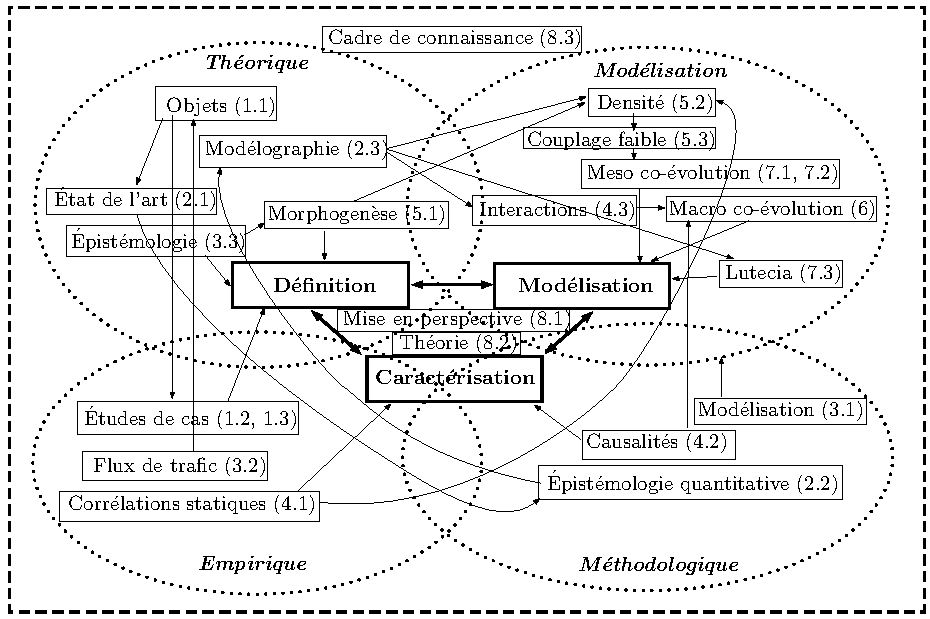
\includegraphics[width=\linewidth]{Figures/Theory/orga.pdf}
	\medskip
	\framecaption{\textbf{Perspective on the organisation.}}{\textbf{Relecture de l'organisation à la lumière des domaines de connaissance.} Nous plaçons au coeur le triptyque issu de la problématique générale de définition, caractérisation et modélisation de la co-évolution. Différentes composantes irriguent ses éléments qui sont indissociables, et soudés finalement par la conclusion et ouverture. Les sections sont placées à titre indicatif dans le domaine de connaissance qui leur correspond le plus (sachant qu'elles sont toutes à cheval sur plusieurs domaines). Les domaines de données et outils sont laissés de côté ici pour faciliter la lecture (et nécessiteraient un découpage plus précis du travail). Les relations entre composantes sont également données à titre indicatif et ne sont pas exhaustives, mais permettent de se rendre compte de la complexité de l'articulation globale.\label{frame:opening:organisation}}
	\end{mdframed}
\end{figure}
%%%%%%%%%%%%%%




Notre travail peut également se placer dans une perspective plus large. Précisons la ``méta-articulation'' de notre travail, c'est à dire la structure implicite des divers développements et ouvertures et donc le cadre global dans lequel s'inscrit le coeur (trois premières parties). L'Encadré~\ref{frame:opening:perspective} schématise cette articulation. Le coeur, qui consiste en la réponse à la problématique, est constitué de trois axes en interaction forte : la définition, la caractérisation et la modélisation de la co-évolution des réseaux de transport et des territoires. Chacun appelle à sa manière des développements dans divers champs\footnote{Nous n'utilisons pas le terme domaine ici pour ne pas entrainer une confusion avec les domaines de connaissance, ceux-ci étant mobilisés différemment comme nous le verrons en Annexe~\ref{app:reflexivity}.} : des développements épistémologiques et en épistémologie quantitative, principalement liés à l'aspect de définition ; des développements de cadres systémiques, induits par les problématiques liées à la modélisation ; et des développements thématiques liés à la caractérisation.

Détaillons le contenu de chacun de ces développements, en les reliant au contenu correspondant principalement en Annexes :
\begin{enumerate}
	\item Epistémologie quantitative : principalement en lien avec les méthodes et outils de revue systématique et d'exploration d'un paysage scientifique en~\ref{ch:modelinginteractions}, nous incluons le cas d'étude original qui a initié la méthode, le corpus du journal Cybergeo, en~\ref{app:sec:cybergeo}, ainsi qu'une application à un corpus massif de brevets en~\ref{app:sec:patentsmining}.
	\item Epistémologie : la mise en contexte de l'étude de Cybergeo avec d'autres approches complémentaires permet une prise de recul épistémologique dans~\ref{app:sec:cybergeonetworks} ; nous amorçons également une réflexion sur les liens entre Economie et Géographie en~\ref{app:sec:ecogeo}.
	\item Cadres systémiques : un cadre de connaissance, contribuant à organiser une connaissance complexe, a déjà été proposé en~\ref{sec:knowledgeframework} ; un cadre formalisant le couplage des modèles des systèmes socio-techniques, suggérant des pistes de formalisation du cadre de connaissance, est développé dans~\ref{app:sec:csframework} ; un cadre pour l'étude de la robustesse des évaluations multi-attributs est développé dans~\ref{app:sec:robustness}.
	\item Thématique : les études de cas des systèmes de transport effectuées en \ref{sec:reproducibility} et en~\ref{sec:energyprice} permettent en l'occurence une confirmation des échelles pertinentes ; l'étude de la génération de données synthétiques,  en lien avec la méthodologie développée en~\ref{sec:computation}, est faite en~\ref{app:sec:syntheticdata} pour la méthode et en~\ref{app:sec:syntheticdata-finance} pour un exemple d'application ; la modélisation des dynamiques migratoires au sein du Delta de la Rivière des Perles ébauchée en~\ref{app:sec:migrationdynamics}, introduit une piste de modèles multi-échelle et raffine les interactions entre villes au niveau des flux individuels.
\end{enumerate}


%%%%%%%%%%%%%%
\begin{figure}
	\begin{mdframed}
	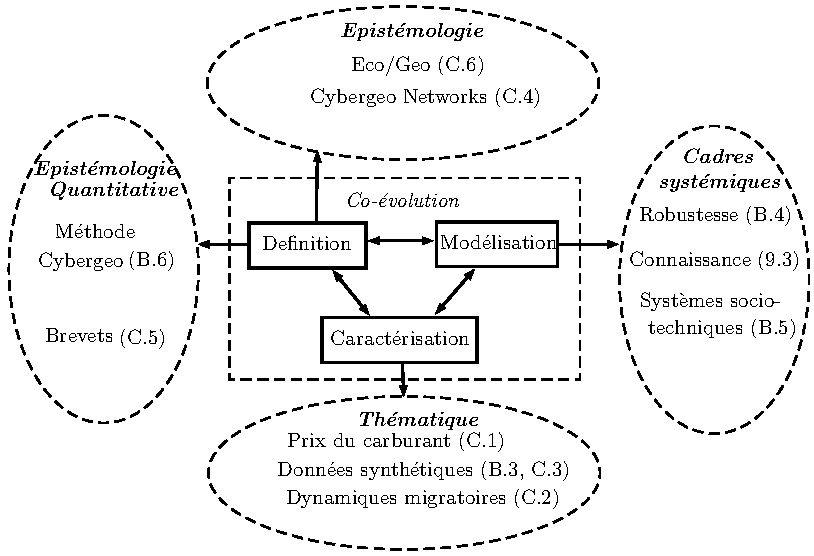
\includegraphics[width=\linewidth]{Figures/Theory/metacadre_norefs.pdf}
	\medskip
	\framecaption{\textbf{Perspective on the global frame.}}{\textbf{Mise en perspective du cadre global.} Le coeur de la problématique, la co-évolution, est composé de trois composantes qui appellent des extensions dans des champs divers (leurs intersections n'étant pas représentées pour faciliter la lecture). Nous y listons dans chaque les différentes ouvertures, menées principalement en Annexes.\label{frame:opening:perspective}}
	\end{mdframed}
\end{figure}
%%%%%%%%%%%%%%



Ces différents champs sont bien sûr à intersections non vides (le cadre de connaissance de~\ref{sec:knowledgeframework} relève par exemple à la fois du cadre systémique et de l'épistémologie, ou l'étude des brevets est un important aspect thématique en lien avec la théorie évolutive des villes) et en interaction : les études d'épistémologie quantitative informent l'épistémologie, qui guide les études thématiques, qui peuvent être mises en perspective dans les cadres systémiques, qui eux dépendent également du positionnement épistémologique.

Ainsi, nous mettons en évidence une structure plus globale pour notre travail, qui dessine en partie la structure d'un projet de recherche que nous détaillerons par la suite.



% \paragraph{External integration}
%At all stages of my thesis project, different types of reflexivity play a crucial role and allow to enlarge the scope of results and theories constructed. I also led some auxiliary projects with aim to increase the integration of my work within disciplines and knowledge domains. For example, in the domain of methodology, \cite{raimbault2017discrepancy} investigates the quantification of robustness of multi-attribute optimisations, that can apply to any type of complex systems. Scientific communication is also a crucial aspect for socio-technical systems, and \cite{raimbault2016game} is an exploration of using agent-based modeling to transmit concepts in ecology. The work of \cite{raimbault2016indirect} was done in the frame of the collaborative development of an interactive platform to explore scientific corpuses, with the aim to promote open science and reflexivity. % These two examples are in the domain of tools, which both can apply to our work and link it to broader fields. 
%Finally, I also explored empirical questions close to my research subjects, such as technological innovation. The diffusion of innovations between cities is indeed one crucial components of the Evolutive Urban Theory. In \cite{bergeaud2017classifying}, we extended the corpus analysis tools to apply to the full corpus of US Patents spanning 1976-2012, to create an endogenous classification that we show to be complementary to the existing office classification. This opens ways for future projects, as the combination with existing inventor localisation databases is a potential candidate for empirical testing of the diffusion hypothesis of the Evolutive Urban Theory. Such a knowledge loop is an illustration how integration of fields can be beneficial. 






\subsection*{Open questions}{Questions ouvertes}


Nous développons à présent des questions fondamentales qui ont été abordées ou ouvertes tout au long de notre travail, que nous classons en trois axes : pratique scientifique (épistémologie appliquée), modélisation et fondements des systèmes complexes spatiaux.


\subsubsection*{Applied Epistemology}{Epistémologie appliquée}


\paragraph{A Truly Open Science}{Pour une science totalement ouverte}

Un premier axe de développement crucial pour l'ensemble de l'écosystème de production de connaissance dans lequel nous nous inscrivons (voir chapitre~\ref{ch:positioning}) est la contribution à une ouverture maximale de la pratique scientifique, c'est à dire la combinaison de l'ensemble des approches résumées par \cite{fecher2014open}, en particulier les aspects démocratique et public qui encouragent l'accès de tous à la production de connaissance et à ses résultats\footnote{Sachant que l'ouverture des produits de la connaissance est évidente dans une perspective complexe, puisque comme le souligne \cite{morin1991methode}, nos idées prennent une certaine indépendance dans la noosphère et ne nous appartiennent pas.}, et les aspects pragmatique et d'infrastructure qui appuient l'efficience augmentée dans un cadre ouvert.

La transparence et mise en disponibilité des données brutes ou au moins pré-traitées, et du code informatique produisant les sorties de simulation ou les figures, semble être plutôt l'exception que la règle en géographie. Comme le rappelle \cite{banos2013pour} qui y dédie l'un de ses principes, ``le modélisateur n'est pas le gardien de la vérité prouvée'', et comme rappelé en~\ref{sec:reproducibility}, une reproductibilité parfaite des résultats est nécessaire pour une reconnaissance d'une quelconque valeur par la communauté scientifique, comme une théorie qui ne fournit pas de possibilité de falsification ne peut être considérée comme scientifique au sens de \noun{Popper}. Des experiences de revue pour \emph{Cybergeo} ont confirmé à l'unanimité ce problème fondamental. Rappelons que la revue \emph{PNAS} exige les données brutes et tableau produisant toute figure, pour prévenir tout biais de visualisation qu'il soit volontaire (ce qui est rédhibitoire et conduit à un signalement) ou non.

Par ailleurs, la communication scientifique est un aspect important de la Science Ouverte. Le mode actuel de publication scientifique est loin d'être idéal. Un article n'est pas un format compréhensible ni vraiment reproductible, et pousse au biais. L'écriture d'un article en répondant au normes de façon à être accepté peut être assimilé à ``un jeu'' dont les règles sont subtiles et qu'il faut maitriser pour faire carrière. Selon notre positionnement, un tel mode de communication est contraire à l'honnêteté et l'intégrité intellectuelle nécessaires à une science éthique et ouverte. Les initiatives se multiplient pour proposer des modèles alternatifs : la revue post-publication en est une, l'utilisation de systèmes de contrôle de version et de dépôts publics une autre, ou la publication éclair de pistes de recherche\footnote{Voir par exemple le \emph{Journal of Brief Ideas} à \url{http://beta.briefideas.org/about}. Les descriptions courtes de pistes de recherche sont souvent reléguées à la discussion ou la conclusion des articles, qui s'écrivent de manière conventionnelle, souvent avec un biais pour justifier a posteriori l'intérêt de \emph{sa nouvelle méthode} qu'il faut malheureusement vendre. On fait alors des plans sur la comète, propose des développements ayant peu de rapport, ou des domaines d'application \emph{qui auront un impact} (lire qui sont à la mode ou qui reçoivent le plus de financements à la période de l'écriture). Ce manuscrit tombe bien évidemment partiellement sous ces critiques, comme les articles qui lui sont associés.}. Par exemple, \cite{bon2017novel} décrit une expérience d'articles dynamiques évalués de manière ouverte par la communauté, avec des métriques associées permettant de faire émerger les travaux jugés intéressants.

% Journal of Design and Science ; Journal mec Paris Sud (CEA ?)


De la même façon, nous soutenons qu'une présentation linéaire d'un projet de recherche est trop fortement réducteur, et que l'invention de modes de communication alternatifs est un enjeu futur pour la Science Ouverte. On peut par exemple imaginer des réseaux interactifs, traduisant la structure de la connaissance sous-jacente, et dans lesquels le lecteur peut naviguer entre les concepts et les analyses, être renvoyé directement vers les données, modèles et analyses. Les grilles de lecture principales en accord avec l'argument que prendrait une explication linéaire peuvent alors être superposées au réseau pour revenir à un mode plus classique de lecture. Une communication par le jeu est également une alternative crédible, notamment dans le cas d'une communication pour le public, et nous en donnons une illustration pour un problème d'écologie en Annexe~\ref{app:sec:mediationecotox}.


\paragraph{For an evidence-based science}{Pour une science Evidence-based}

Nous postulons qu'une science entièrement \emph{evidence-based}, quel que soit son objet, est possible et souhaitable en articulation avec la science ouverte. L'idée est de chercher à déconnecter la connaissance scientifique de tout dogmatisme, de tout a priori politique et de tout jugement de valeur\footnote{Sachant que par ailleurs ceux-ci doivent être plus que jamais développés et réfléchis pour articuler la science avec la société, mais doivent le moins possible interférer avec le processus de production de connaissance en lui-même. Suivant \cite{morin2004methode}, une éthique de la connaissance et une pensée complexe induit naturellement une éthique plus large, permettant l'autonomie de la connaissance scientifique sans la rendre inhumaine.}. Dans le cas de l'étude de sujets en lien avec des individus ou des sociétés (c'est à dire les sciences humaines), un tel positionnement n'est possible selon \cite{morin1991methode} que par le passage par l'établissement d'un ``méta-point de vue'', c'est à dire par une certaine réflexivité qui permet au connaisseur de comprendre sa position et sa propre démarche. Nous donnons des pistes pour la construction de tels points de vue, sous la forme de ce que nous appelons \emph{perspectivisme appliqué}, en Annexe~\ref{app:sec:cybergeonetworks} ainsi qu'en Annexe~\ref{app:sec:csframework} pour une piste de formalisation.


Cette problématique est directement reliée à la question récurrente de la dichotomie ``qualitatif-quantitatif'', que nous jugeons peu pertinente dans le cadre de sciences intégratives. En effet, si la dichotomie se base sur une différence entre objectif et subjectif, nous rappelons que toute connaissance est subjective, et que celles où le rôle du sujet est particulièrement déterminant peuvent ``s'objectiver'' par la prise du méta-point de vue, par exemple par le couplage avec d'autres approches, c'est à dire précisément par la prise d'une position intégrative. Si elle se base sur une question de nature des données, elle n'est que partiellement pertinente puisque la limite est floue : un texte d'interview peut très bien faire l'objet d'analyse textuelle alors qu'une régression doit être interprétée qualitativement. En fait, nous pensons qu'il existe différentes méthodes plus ou moins appropriées selon la connaissance à produire (voir par exemple \cite{gros2017quantifier} qui fustige l'utilisation de statistiques inférentielles pour un corpus ethnographique), mais qu'il n'y a pas ``chasse gardée'' de telle discipline sur telle méthode et que les couplages et transferts seront toujours plus nécessaires à l'avenir.


%%%%
%% -- ON HOLD -- : hardcore
%Le mantra du mariage entre qualitatif et quantitatif est asséné mécaniquement par de nombreux auteurs, mais lorsqu'il s'agit de mise en application, on peut se permettre de soupçonner dans le meilleur des cas une naïveté, dans le pire des cas une hypocrisie. Quel sens à faire semblant de faire des analyses quantitatives en tartinant des pages de régression linéaires dont le $R^2$ ne dépasse pas 0.1 ?  % find thèse which Renaud was talking about
% Quel sens à simuler à grande échelle des Gaussiennes pour en calculer la moyenne ?\footnote{au moment de l'écriture, l'application étrange était toujours en ligne à \texttt{http://shiny.parisgeo.cnrs.fr/gibratsim/}, onglet simulation, malgré des signalements répétés} % maybe not do bad pub, insist on other noce aspects of the application ? ; surtout ne pas citer cette merde. Quel sens à faire semblant de détenir une connaissance qualitative fine pour justifier la mise en place de modèles relevant de l'usine à gaz technocratique ?\footnote{cette remarque est partiellement une auto-critique, puisqu'il faut rappeler le caractère très peu qualitatif de notre travail}
%\comment{sur l'evidence-based : même le subjectif est objectif en un sens ? question d'honneteté et d'intégrité intellectuelle - lié nature connaissance, à developper. arreter les arnaques quel que soit le type de méthode, rigueur et reproducibilité à mettre en place.}
%\comment{in link ``Complexity, Complexities, and Complex Knowledges'', importance of Nature of Complexity ?}
%\comment[JR]{evoquer ouverture des cours, formation interdisciplinaire etc. : pas ici, plutot en ouverture finale ?}

% needs to do experiments to apply knowledge framework.
%  -> exemples : - MigrationDynamics
%                - SimpopSan
%


\paragraph{Quantitative epistemology}{Epistémologie quantitative}

% - full-text mining ?
% - integrated platform -> mention here CybergeoNetworks ?
%

Les points précédents doivent être traités conjointement avec l'utilisation de méthodes d'épistémologie quantitative permettant une réflexivité accrue, comme par exemple la méthode par hyperréseau utilisée en~\ref{sec:quantepistemo}, appliquée au corpus Cybergeo en~\ref{app:sec:cybergeo}, à un corpus de brevets en~\ref{app:sec:patentsmining} et à notre propre travail en~\ref{app:reflexivity}. La plateforme CybergeoNetworks\footnote{Accessible à \url{http://shiny.parisgeo.cnrs.fr/cybergeonetworks/}.} est une collaboration dans cette direction, présentée en détails en~\ref{app:sec:cybergeonetworks}. Elle permet notamment la prise d'autonomie par les auteurs mais également par les journaux libres qui peuvent alors rivaliser avec les entreprises prédatrices d'édition qui valorisent à leur profit les analyses de corpus.




%%%%%%%%%%%%%%%%
\subsubsection*{Modeling}{Modélisation}

Sur le plan de la méthodologie de la modélisation, nous donnons des axes précis complémentaires à ceux mis en place par~\cite{pumain2017urban} (multi-modélisation, exploration des modèles).


\paragraph{Coupling models}{Couplage des modèles}

% - questions ouvertes sur le couplage, enjeux, def possibles, etc.
% - link dynamical systems/ABM

La définition du couplage de modèles ou d'approches, et notamment du degré de couplage (couplage fort ou couplage faible) dépend des cadres utilisés et n'a pas forcément de fondement théorique. La construction de théories permettant une telle définition qui serait par ailleurs opérationnelle est une question ouverte. Une approche possible utilise par exemple les rapports entre complexités de Kolmogorov des différents modèles concernés. Une approche formelle est donnée en~\ref{app:sec:csframework} pour le couplage de perspectives. Cette approche est profondément liée aux questions épistémologiques, puisqu'il pourrait s'agir d'une manière de formaliser la logique du cadre de connaissance.


La question du couplage de modèles hétérogènes est bien sûr liée : dans quelle mesure est-il pertinent de choisir tel ou tel type de modèle et comment les coupler ? \cite{banos2015coupling} l'illustre pour un modèle épidémiologique, couplant un modèle classique par équations différentielles à un modèle de microsimulation. Le lien entre modèles agents et système dynamiques peut être établi dans certaines configurations, comme nous l'avons fait pour le modèle de Simon et le modèle de Gibrat en~\ref{app:sec:stochurbgrowth}, mais la question de classes de problèmes pour lesquels des liens seraient systématiques ou non reste une question ouverte.


Enfin, la nécessité du benchmarking de modèles comparables a été soulevée depuis un certain temps \cite{axtell1996aligning}, mais reste très peu appliquée : le développement d'outils et de méthodes facilitant de telles comparaisons est également un point important.



\paragraph{Empowering Models of Simulation with validation and assessment tools}{Construire des outils de validation pour les modèles de simulation}

% -> robustness
% -> empirical AIC
% Note : sur le seed, on est un peu evasifs. etre plus explicite ? (cf Clem spaceMatters)


L'essentiel de l'entreprise d'OpenMole est orientée dans ce but de construction d'outils et de méthodes pour la validation des modèles. Nous contribuons à cet effort dans notre travail, par exemple en~\ref{sec:interactiongibrat} par la construction d'un critère de sur-ajustement, ou en~\ref{app:sec:robustness} par l'élaboration d'une mesure de la robustesse d'un modèle aux données manquantes. L'étude du comportement des modèles par rapport au sur-ajustement, notamment dans le cadre de la multi-modélisation, est un enjeu fondamental pour le développement futur de ces approches.





\subsubsection*{Foundations of spatial complex systems}{Fondements des systèmes complexes spatiaux}

Certaines questions fondamentales ont été suggérées au sujet des systèmes complexes ayant une structure spatiale.

\paragraph{Non-stationarity, non-ergodicity and path-dependancy}{Non-stationnarité, non-ergodicité et dépendance au chemin}

% - link geosim/spatial stat/economics

Le lien entre non-stationnarité spatiale et/ou temporelle et non-ergodicité, pouvant éclairer les propriétés de dépendance au chemin, n'a à notre connaissance pas été étudié systématiquement, au moins dans le cadre des systèmes territoriaux. Nous suggérons qu'un lien accru entre géosimulation, statistiques spatiales et économie géographique, contribuerait à la compréhension de ce type de question.



\paragraph{Multi-scale Models}{Modèles Multi-scalaires}

% coupling between scales.

Comme nous l'avons déjà amplement répété, il existe très peu de modèles des systèmes territoriaux effectivement multi-scalaires, et leur développement à des échelles pertinentes et à un degré de complexité raisonnable, est également un défi futur important.

% -- ON HOLD --
%\paragraph{Towards Operational Models}{Vers des Modèles Opérationnels}
% Concrete operationalization of models : is it desirable ? what needed to reach it ?


\paragraph{Methodological standards}{Standards méthodologiques}

% For the application of suited methods : ex not use hierarchical clustering for time-series, not use linear models when not suited, fit well a power law -> on that, try to apply golden standard (Crutchfield) to existing works (cf thèse Olivier) and look if conclusions hold

Enfin, un effort considérable doit être fait, particulièrement en géographie, pour respecter des standards méthodologiques a minima : par exemple utilisation de classifications de séries temporelles appropriées~\cite{liao2005clustering}, ajustement de loi puissances sur des données empiriques selon la méthode standard de \cite{clauset2009power} et non une simple régression des moindres carrés, utilisation de modèles non-linéaires si besoin.



%%%%%%%%%%%%%%%%%
% Other possible developments


%Other targeted projects such as the exploration of an hybrid macro-economic/accessibility-based model to explore transportation companies line implementation strategies are still at the state of ideas and are not described here.


%
%\comment{lister les principaux contributeurs etc. ; quoi est compatible avec quoi quest ce quon pourrait coupler etc ; faire analyse epistemo quanti.}




\stars


%----------------------------------------------------------------------------------------

%\newpage


%%%%%%%%%%%%%%%%%%%%%%%%
\section*{Towards a Research Program}{Vers un programme de recherche}

\label{sec:researchprogram}


\subsection*{For an Integrated Geography}{Pour une Géographie Intégrée}

% develop here position for a renewal of TQG : additional three dimensions in the knowledge framework ; position at the core of fundamental CS - cannot ignore fundamental questions.




\bpar{
}{
Comme déjà souligné en~\ref{sec:epistemology}, les bouleversements techniques et méthodologiques qu'une discipline peut subir sont souvent accompagnés de profondes mutations épistémologiques, voire de la nature même de la discipline. Il est impossible de juger si l'état actuel des connaissances est transitoire, et s'il l'est quelle est le régime stable qui terminerait la transition s'il en existe un.
}

\bpar{}{
La spéculation est le seul moyen de lever partiellement le voile, sachant que celle-ci sera nécessairement auto-réalisatrice : proposer des visions ou des programmes de recherche oriente les moyens et questions. L'incomplétude théorique en physique, lorsqu'il s'agit par exemple de lier relativité générale et physique quantique, c'est à dire le microscopique stochastique au macroscopique déterministe, orientent les visions du futur de la discipline qui elle-même conditionnent les actions concrètes qui dans ce domaine sont indispensables (financement du CERN ou de l'interféromètre d'ondes gravitationnelles spatial LISA).
}

\bpar{}{
En géographie, même si les investissements techniques sont incomparables, ceux-ci existent (accès aux moyens de calcul, financement de laboratoires intégrés, etc.) et sont déterminés également par les perspectives pour la discipline. Nous proposons ici une vision et un manifeste d'une nouvelle géographie, qui est déjà en train de se faire et dont les bases sont solidement construites petit à petit. L'aventure de l'ERC Geodivercity \cite{pumain2017urban} en est l'allégorie, d'autant plus qu'elle a confirmé la plupart des directions proposées par~\cite{banos2017knowledge}. L'intégration de la théorie, de l'empirique, de la modélisation, mais aussi de la technique et de la méthode, n'a jamais été aussi creusée et renforcée que dans les divers développements du projet. Sans l'accès à la grille de calcul et aux nouveaux algorithmes d'exploration permis par OpenMole, les connaissances tirées du modèle SimpopLocal auraient été moindres, mais les développements techniques ont aussi été conduits par la demande thématique.
}


\bpar{
}{
Nous appuyons le fait que le cadre de connaissance proposé en~\ref{sec:knowledgeframework} est particulièrement favorable à une application à la continuité contemporaine de la Géographie Théorique et Quantitative. Ce cadre permet en effet de répondre aux contraintes suivantes : (i) transcender les frontières artificielles entre quantitatif et qualitatif ; (ii) ne pas favoriser de composante particulière parmi les moyens de production de connaissance (aussi divers que l'ensemble des méthodes qualitatives et quantitatives classiques, les méthodes de modélisation, les approches théoriques, les données, les outils), mais bien le développement conjoint de chaque composante.
}


\bpar{}{
Nous rappelons que le cadre étend celui de~\cite{livet2010}, qui consacre le triptyque des domaines empiriques, conceptuels et de la modélisation, en y ajoutant les domaines à part entière que sont les méthodes, les outils (qu'on peut voir comme des proto-méthodes) et les données. Toute démarche de production de connaissance, vue comme une \emph{perspective} au sens de~\cite{giere2010scientific}, est alors une combinaison complexe des six domaines, les fronts de connaissance dans chacun étant en co-évolution.
}

\bpar{}{
Nous postulons que l'application de notre cadre de connaissance est de mise avec l'émergence d'une \emph{Géographie Intégrée}, que nous nommons ainsi pour souligner à la fois l'intégration des différents domaines mais aussi des connaissances qualitatives et quantitatives, puisque les deux se fondent dans chacun des domaines.
}

% other illustration : neural networks-deep learning-cuda etc : coevol of methodo, tools, etc (includes Hardware -> as tools or should be a different domain.. ?)
% the CybergeoNetworks is also a good illustration.







%%%%%%%%%%%%%%%%%%%%%%%%
\subsection*{Research project}{Projet de recherche}

% le projet postdoc étendu : AI / th geo / epistemo
% presentation White sur l'AI



% My long term research objective is therefore to construct \emph{Integrative Theories} for Territorial Systems, in the sense of an integration of fields (horizontal integration of the Complex Systems roadmap \cite{2009arXiv0907.2221B}), an integration of scales (vertical integration of the roadmap) which is one of the main missing leg in my thesis, and an integration of Knowledge Domains through different types of reflexivity. I plan therefore my future research as a continuation of my thesis work in its purpose and spirit, in particular by conjointly advancing knowledge in the field of urban systems and at a general level by continuing producing theories, methodologies and tools applying to complex systems in general. The project is articulated around one main axis and two auxiliary directions, with a strong interdependency between each.

%The principal question I propose to investigate is to dig further into the non-stationarity, non-ergodic and multi-scalar nature of territorial systems, and how these can be better understood conjointly and taken into account in existing approaches. The fundamental difficulties in studying territorial systems raise from the combination of regularities in involved processes with the essential role of local particularities, making stationarity or ergodicity properties impossible. The heterogeneity of components of such socio-technical systems is also combined with their manifestation at different time and spatial scales. The main theoretical, empirical and practical difficulties encountered in our thesis can somehow be related to these questions. I postulate that a powerful entry to it is the tentative of constructing bridges between geographical theories of territorial systems in the spirit of the Evolutive Urban Theory and Scaling Theories of Cities. The first emphasize particularities of territorial entities whereas the second focuses on universal laws, and both provide credible explanations for scaling laws. Open questions to bridge these theories can for example include: (i) find endogenous modular decompositions of territorial systems and corresponding scales that make local derivations of growth from scaling laws compatible with a global non-ergodicity; (ii) couple models from both theories at different scales, to test for stationarity of different components. I already started a collaboration that could inform the second point, on an agent-based model for the establishment of a circular economy network embedded within a city system. The first point will be the subject of the concrete core project during the postdoctoral positions, for which a suggestion of methodology and steps can be: (i) proceed to a systematic review and meta-analysis of studies and datasets studying scaling laws; (ii) on spatially consistent consolidated datasets, investigate endogenous stationarity scales using for example optimal fitting range methods; (iii) construct an interaction models between territorial subsystems, similar to models inspired from the Evolutionary Urban Theory I already developed, that would at an upper level determine local parameters for the Scaling theory. The already suggested investigation of the diffusion of innovation through our Patent semantic classification database would be an interesting way to externally validate this model.


Nous détaillons finalement un projet de recherche à long terme qui (i) s'inscrit dans la continuité de cette monographie ; (ii) s'inscrit dans le cadre d'une géographie intégrée, et plus généralement d'une intégration verticale et horizontale, mais aussi des domaines et des types de connaissance ; (iii) s'attaque à un certain nombre de questions ouvertes mentionnées ci-dessus ; et (iv) est intrinsèquement réflexif et complexe.


%\paragraph{Towards a global take on urban systems}{Vers une compréhension globale des systèmes urbains}

\bpar{
The aim would be to solve a multi-scale geographical problem, that is to understand how and when interdependencies between cities have built regional systems of cities and to identify the most probable scenario of their potential coalescence as a consequence of globalisation processes. These high-level questions have direct practical implications for measuring global and local inequalities and managing urban growth.
}{
Le couplage multi-échelle des modèles urbains suggéré en~\ref{sec:contributions} peut en fait se projeter dans une problématique plus globale. L'idée serait d'aborder un problème géographique multi-échelle, qui est de comprendre comment et quand les interdépendances entre les villes ont conduit à l'émergence de systèmes régionaux de villes, et d'identifier le scenario le plus probable de leur fusion potentielle comme conséquence des processus de globalisation. Ces questions abstraites ont des implications directes pour la mesure des inégalités globales et locales et la gestion de la croissance urbaine.
}

\bpar{
The principal question we propose to investigate finds roots in the multi-scalar nature of territorial systems. Converging evidence suggest the relative independent historical development of regional urban systems across the world, and an increased interdependency between these in the processes of globalisation. Can we already quantify these at different scales ? How does the coupling and the opening of subsystems operate, and what are its most plausible consequences, from convergence of dynamics to an increase of inter- and intra-subsystems inequalities ?
}{
Cette question trouve sa source dans la nature multi-échelle des systèmes territoriaux. Des résultats convergents suggèrent une certaine indépendance du développement historique des systèmes urbains régionaux tout autour du monde, et une interdépendance accrue entre ceux-ci dans les processus de globalisation. Est-il possible de déjà les identifier à différentes échelles ? De quelle manière le couplage et l'ouverture des sous-systèmes s'opère, et quelles sont ses conséquences les plus plausibles, de la convergence des dynamiques à l'augmentation des inégalités inter et intra système ?
}


\bpar{
We postulate that a powerful entry to this research question is the construction of bridges between geographical theories of territorial systems in the spirit of the Evolutive Urban Theory and Scaling Theories of Cities. The first emphasize particularities of territorial entities whereas the second focuses on universal laws, and both provide credible explanations for scaling laws. A strategy to answer the question and combining both would consist in: (i) finding endogenous modular decompositions of territorial systems and corresponding scales, and quantifying their universality through inter and intra scaling; (ii) modeling this multi-scalar system by coupling models of urban growth, that would be validated through scaling properties. The models developed here are good candidates as sub-models, since co-evolution inside and between scales is a characteristic feature of complex urban systems.
}{
Nous postulons qu'une entrée puissante pour cette question de recherche est la construction de ponts entre les théories géographiques des systèmes territoriaux dans l'esprit de la théorie évolutive des villes~\cite{pumain1997pour} et de la théorie du \emph{Scaling}~\cite{west2017scale}. La première appuie les particularités des entités territoriales tandis que la seconde se concentre sur des lois universelles, et chacune fournissent des explications crédibles aux lois d'échelles urbaines. Une stratégie pour répondre à la question tout en combinant les deux théories consisterait en : (i) la mise en évidence empirique de décompositions modulaires des systèmes territoriaux et des échelles correspondantes, et la quantification de leur universalité par le scaling intra- et inter-système ; (ii) la modélisation de ce système multi-échelle par le couplage de modèles de croissance urbaine, qui seraient validés par les propriétés de scaling. Les modèles que nous avons développé ici sont de bons candidats comme sous-modèles, puisque la co-évolution au sein et entre les échelles est une caractéristiques des systèmes urbains complexes, comme nous l'avons montré.
}





\bpar{
An auxiliary research direction that I will conjointly tackle is the exploration of potential relations between territorial systems and artificial intelligence. It comes naturally as a corollary and is informative for the main question, for at least two very different reasons. The first is rather practical and linked to the emergence of ubiquitous information and computing in cities, that some observers design as ``smart cities'': the new large datasets available have been proven to be a powerful analysis tool as witness the numerous recent works by physicists on cities for example, and these new urban behavior may probably induce some regime changes partly because of of their self-fulfilling nature. The second is more difficult to grasp: the importance of morphogenesis in my current understanding of territorial systems and the possible application of this concept at different levels such as knowledge production. Morphogenesis can be used to conceptualize both the evolution of territories and of ideas: to what extent the emergence of territories contains an endogenous intelligence. The success of using slime mould network generation in my thesis, which have been shown otherwise to be powerful computation tools, is an other clue of a possible connexion.
}{
Deux axes de recherches sous-jacents apparaissent alors comme nécessaires à la cohérence globale du projet. Le premier consiste en l'exploration des relations potentielles entre les systèmes territoriaux et l'intelligence artificielle. Celui-ci vient comme corollaire et enrichit la question principale pour au moins deux raisons très différentes. La première est plutôt pratique et liée à l'émergence de l'information et du calcul omniprésents dans les villes, qui peuvent être compris comme participant à l'émergence des \emph{smart cities} \cite{batty2018artificial} : les jeux de données massifs nouvellement disponibles ont été montrés des outils efficaces comme en témoigne la quantité de travaux récents des physiciens sur la ville par exemple, et ces nouveaux comportements urbains peuvent probablement induire des changement de régime en partie à cause de leur nature auto-prophétrice. La seconde est plus difficile à saisir : l'importance que nous avons donné à la morphogenèse et la possibilité d'appliquer ce concept à différents niveaux, notamment celui de la production de connaissance. La morphogenèse peut être utilisée pour conceptualiser à la fois l'évolution des territoires et des idées : dans quelle mesure l'émergence des territoires contient-elle une intelligence endogène ? L'utilisation du modèle de slime mould en~\ref{sec:networkgrowth}, qui est par ailleurs doté de capacités de calcul, et un autre indice d'une connexion possible. Nous notons également la contribution de \noun{White} rapportée en~\ref{app:sec:ecogeo} qui suggère la construction de modèles intelligents et autonomes comme le futur de la modélisation des systèmes territoriaux.
} 

\bpar{
A second auxiliary subject is the theoretical and applied study of knowledge production on Complex Systems. %It also logically follows from many components I already explored or on which I am currently working: I also started a collaboration aiming at a parsimonious spatialized agent-based model for the emergence of language, and more particularly to understand the influence of geography on language differentiation. Cultural evolution is a crucial component for the understanding of knowledge production.
This axis will be necessary to the project, first to continue to enhance the reflexivity and interdisciplinarity through the further development of quantitative epistemology methods and tools such as more elaborated text-mining and meta-analysis tools, and secondly precisely because of reflexivity as concrete case studies such as the aforementioned language evolution precisely apply to territorial systems which main components are cognitive agents.
}{
Un deuxième axe complémentaire est l'étude théorique et appliquée de la production de connaissance sur les systèmes complexes. Cet axe est nécessaire, d'une part pour continuer à favoriser la réflexivité et l'interdisciplinarité par le développement des méthodes et outils d'épistémologie quantitative comme des outils plus élaborés de fouille de textes complets et de meta-analyse, et dans un second temps, précisément grâce à la réflexivité, parce que des cas d'étude potentiels comme l'évolution culturelle (pouvant être étudiée par l'intermédiaire de l'innovation technologique dans la continuité de~\ref{app:sec:patentsmining}, ou de l'évolution du langage sur laquelle une collaboration est en cours) s'appliquent aux systèmes territoriaux dont les principales composantes sont des agents cognitifs.
}


\bpar{
The strongly coupled elaboration of these different components, i.e. their co-evolution, in the exact spirit of what I achieved until now, is necessary for the integrated nature of the project and achieve its objective of integrative theories.
}{
L'élaboration fortement couplée de ces trois différentes composantes, c'est à dire leur co-évolution, dans l'esprit de tout ce qui a été accompli jusque là, est nécessaire pour le caractère intégré du projet et l'atteinte de son objectif de production de théories intégratives des systèmes territoriaux.
}





\stars








%%%%%%%%%%%%%%%%%%%%%%%%%%%%%



%%%%%%%%%%%%%%%%%%%%%%%%%%%%%
% Conclusion




\vfill

\stars

{\raggedleft
\textit{
Cet hiver a des airs de printemps\\
Des peuples ou de l'esprit, au diable l'âme.\\
Le vent se lève, ça faisait longtemps\\
Triste de s'enfermer pour quelques grammes.\\
}
}
\medskip

{\raggedright

\textit{
Cet avenir des airs de passé\\
S'il fallait juste trouver le régime,\\
Assassinée la complexité\\
Maintes perspectives se cachent en les crimes.\\
}
}

\medskip
{\raggedleft

\textit{
Pour une morphogenèse politique\\
Adieu le coron, ses tristes briques\\
Murs qui s'érigent tuent votre espérance.\\
}
}

\medskip
{\raggedright


\textit{
Perle de la mer, sirène hante la crique\\
Du haut des tours s'amuser du cirque\\
L'hiver d'idées qui peuple la France.\\
}
}

\stars

\vfill




%------------------------------------


\newpage






%\chapter*{Conclusion}{Conclusion}
\chapter*{Conclusion}


% to have header for non-numbered introduction
\markboth{Conclusion}{Conclusion}


\headercit{Explorer sans relâche les systèmes géographiques\ldots}{Arnaud Banos}{}

% not appropriate (removed incipit)
% Le lecteur qui aura tenu jusqu'ici et qui a la mémoire solide ou bien sélective, ou encore qui aura adopté un style de lecture roman policier, se plaindra du manque d'originalité dans l'origine des citations introductives.


Notre thèse est un système complexe qui exhibe une finalité auxiliaire déterministe : cette conclusion par un adage de \noun{Banos}. Les principes de son contexte, simples mais efficaces et profonds, traversent en effet ce travail : les ``9 principes de Banos'' sont implicitement présents dans la majorité des travaux menés et perspectives ouvertes. Même si une application idéale de ces principes relèverait d'un ``Démon de Banos'', à l'instar du Démon de Laplace ou de Maxwell, qui serait capable d'articuler interdisciplinaire et disciplinaire sans se perdre tout en respectant l'ensemble des principes, leur appréhension comme utopie scientifique, naturellement réflexive donc évolutive et adaptive, nous semble une entrée puissante pour de nouvelles approches intégratives des systèmes territoriaux. 


Notre contribution épistémologique, méthodologique en lien avec ces points est essentielle, même si celle ci est difficile à expliciter et nécessitera un certain recul pour être effectivement cernée. D'une certaine manière, nous avons apporté une brique supplémentaire comme \emph{proof-of-concept} du système de principes banosien, mais également comme implémentation et approfondissement de celui-ci sur certains points. Nous avons montré que leur application est loin d'être simple, et que toujours guette le risque de sombrer dans le réductionnisme malgré ces principes fondamentalement complexes. Le dixième commandement serait-il alors : \textit{S'efforcer à appliquer ces principes en ne perdant jamais de vue la complexité et le rôle de la réflexivité} ?


Notre contribution thématique n'est pas forcément facile à situer et nécessitera un recul considérable pour appréhender ses implications. Avons-nous résolu le noeud gordien de la co-évolution ? L'avons-nous tranché ? La réponse la plus fidèle serait que nous en avons tranché une partie, celle naïve comprenant la définition dont nous sommes parti en introduction ou les positionnement de type ``poule-et-oeuf'' typique des débats des effets structurants, mais que nous avons noué un autre bien plus considérable, en révélant la complexité de ce concept et de ses manifestations.


Revenant à notre problématique fondatrice, nous rappelons que (i) nous avons donné une définition de la co-évolution propre aux systèmes territoriaux ainsi qu'une méthode opérationnelle de caractérisation ; (ii) nous avons exploré des pistes de modélisation à différentes échelles, qui s'accordent avec un cadre théorique global. Répondre à cette problématique nous a permis par ailleurs de progressivement dégager un cadre plus large et de vastes perspectives de recherche.


Notre modeste mission est accomplie, et un fantastique voyage commence tout juste. L'accomplissement passager devient les fondations de ceux à venir. La cumulativité des connaissances ne s'improvise pas, et nous espérons que le tissu complexe dont nous avons cousu les premières mailles sera assez robuste pour s'y insérer. \textit{la route est longue mais la voie est libre.}




\stars










%%%%%%%%%%%%%%%%%%%%
%% Add epilogue -> may be separated




%\chapter{When Science meets Art}{Quand la science se mêle à l'art} % Chapter title

%\label{app:art} % For referencing the chapter elsewhere, use \autoref{ch:name} 

%----------------------------------------------------------------------------------------


%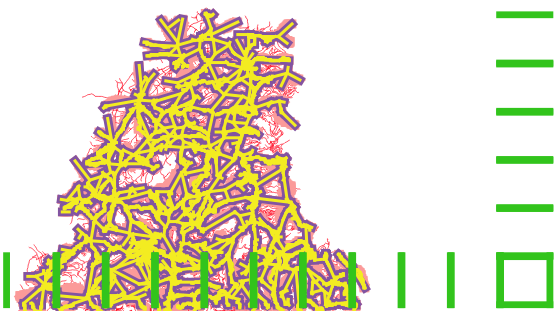
\includegraphics[angle=90]{Figures/Art/Capture d’écran 2016-08-08 à 11.46.55}


\begin{figure}
	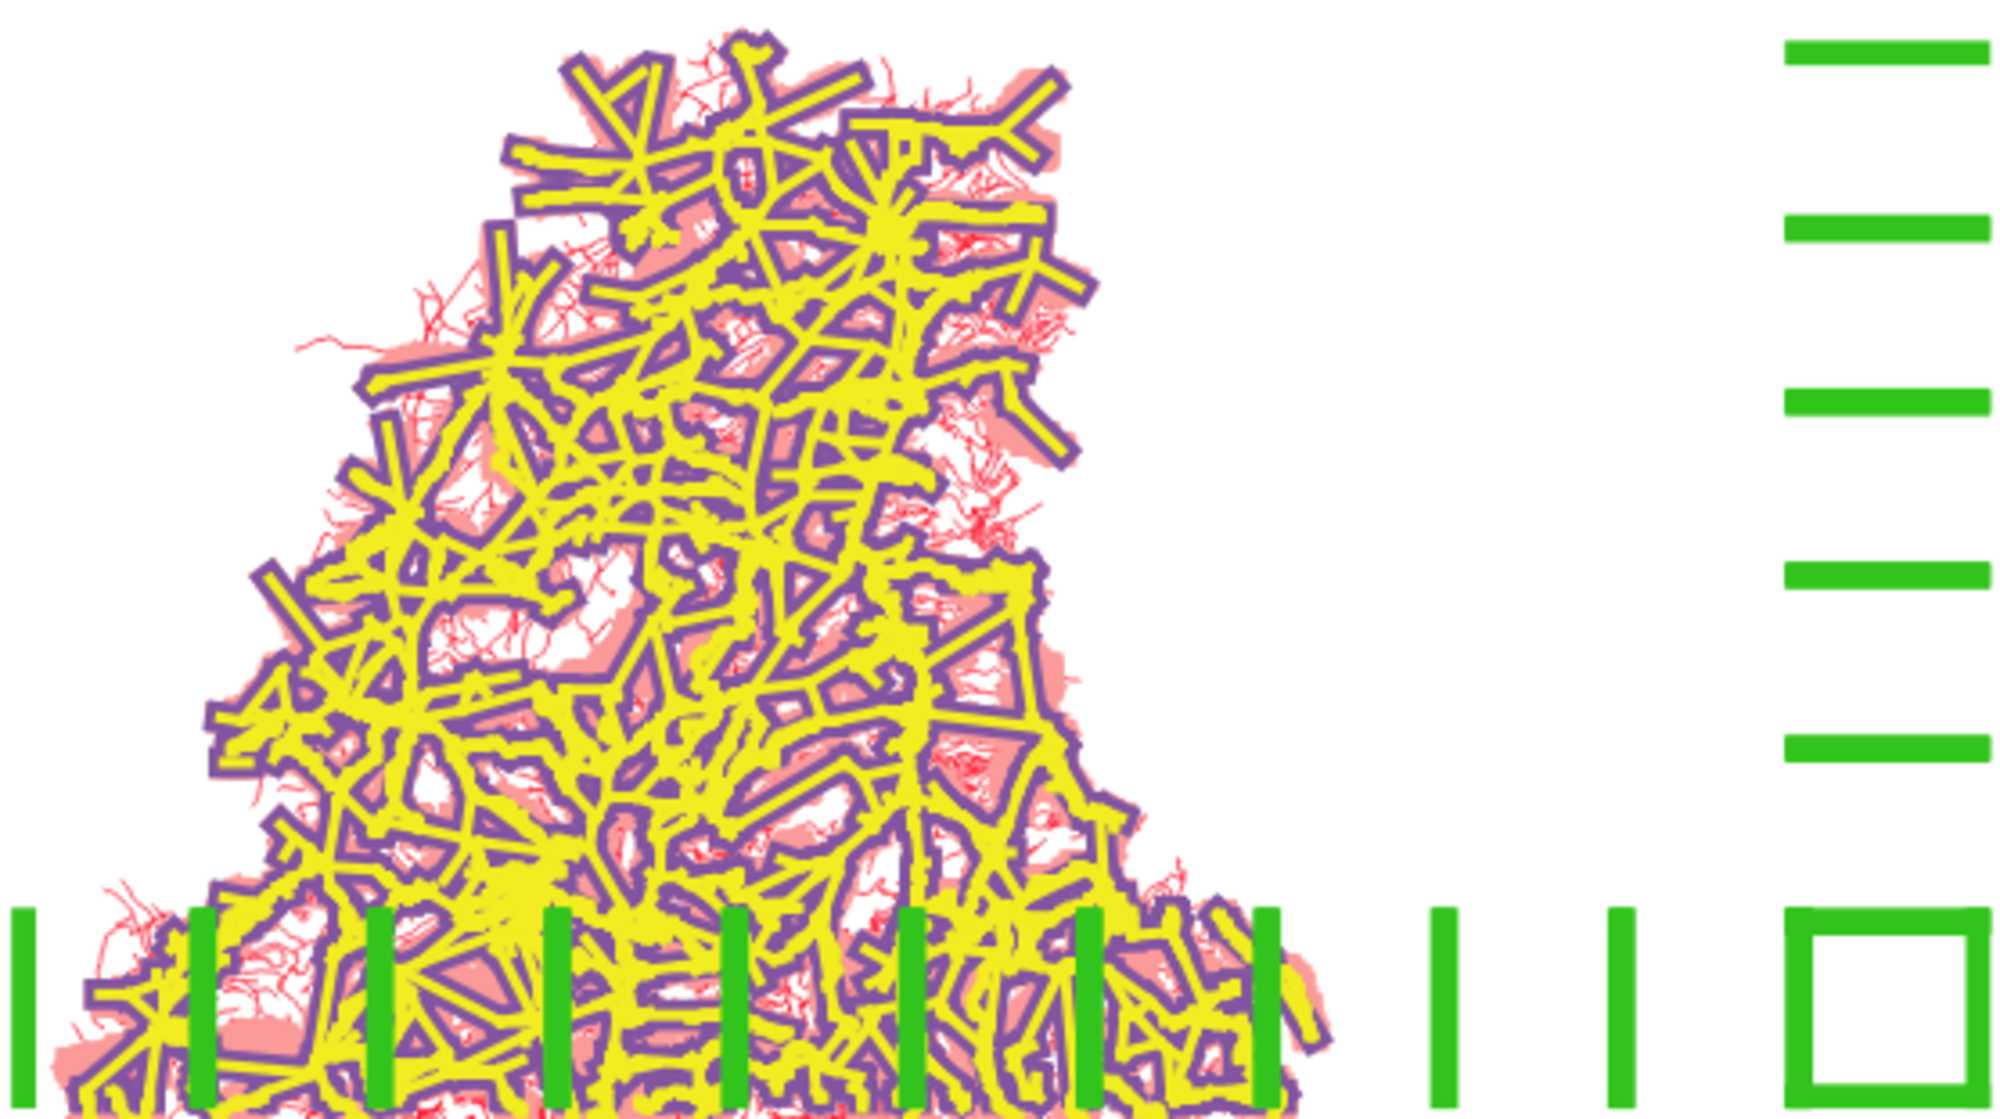
\includegraphics[width=\textheight,angle=90]{Figures/Final/CL-artwork.jpg}
\end{figure}












%%%%%%%%%%%%%%%%%%%%%%%%%%%%%





%------------------------------------------------
% Provisory chapters 





%------------------------------------------------
% Bibliography


\cleardoublepage
% Bibliography

\label{app:bibliography} % Reference the bibliography elsewhere with \autoref{app:bibliography}

\manualmark % Work-around to have small caps also here in the headline
\markboth{\spacedlowsmallcaps{\bibname}}{\spacedlowsmallcaps{\bibname}} % Work-around to have small caps also
\phantomsection
\refstepcounter{dummy}

\addtocontents{toc}{\protect\vspace{\beforebibskip}} % Place the bibliography slightly below the rest of the document content in the table of contents
\addcontentsline{toc}{chapter}{\tocEntry{\bibname}}



\printbibliography
%[title={Bibliographie principale}]

 % Bibliography



%----------------------------------------------------------------------------------------
%	THESIS CONTENT - APPENDICES
%----------------------------------------------------------------------------------------

%\appendix

\ctparttext{}

\part{Appendix} % New part of the thesis for the appendix


%%%%%%%%%%%%%%%%%%
% Appendix A (10) : Supplementary Information
%
%% Technical developments
\chapter{Supplementary Information}{Informations supplémentaires}

\label{app:supplementary} % For referencing the chapter elsewhere, use \autoref{ch:name} 

%----------------------------------------------------------------------------------------


\headercit{C'est hardcore tes calculs.}{Anonyme}{}



This chapter gathers various technical developments, that have the common points to be not essential to the core of the thesis and difficult to digest.



\section{Technical Developments}{Technical Developments}




\subsection{Derivations for Urban Growth Models}{Dérivations pour les modèles de croissance urbaine}





\begin{lemma}
The limit of a Preferential Attachment model when $\lambda \ll 1$ is a linear-growth Gibrat model, with limit parameters $\mu_i(t)=1+\frac{\lambda}{m\cdot (t-1)}$.
\end{lemma}

\begin{proof}

Starting with first moment, we denote $\bar{P}_i(t)=\Eb{P_i(t)}$. Independence of Gibrat growth rate yields directly $\bar{P}_i(t)=\Eb{R_i(t)}\cdot \bar{P}_i(t-1)$. Starting for the preferential attachment model, we have $\bar{P}_i(t) = \Eb{P_i(t)} = \sum_{k=0}^{+\infty}{k\Pb{P_i(t)=k}}$. But
\[
\{P_i(t)=k\}=\bigcup_{\delta=0}^{\infty}{\left(\{P_i(t-1)=k-\delta\}\cap \{P_i\leftarrow P_i + 1\}^{\delta}\right)}
\]

where the second event corresponds to city $i$ being increased $\delta$ times between $t-1$ and $t$ (note that events are empty for $\delta \geq k$). Thus, being careful on the conditional nature of preferential attachment formulation, stating that $\Pb{\{P_i\leftarrow P_i + 1\} | P_i(t-1)=p} = \lambda\cdot\frac{p}{P(t-1)}$ (total population $P(t)$ assumed deterministic), we obtain

\begin{equation*}
\begin{split}
\Pb{\{P_i\leftarrow P_i + 1\}} & = \sum_{p}{\Pb{\{P_i\leftarrow P_i + 1\} | P_i(t-1)=p}\cdot \Pb{P_i(t-1)=p}}\\
&=\sum_{p}{\lambda\cdot\frac{p}{P(t-1)}\Pb{P_i(t-1)=p}}=\lambda\cdot\frac{\bar{P}_i(t-1)}{P(t-1)}\\
\end{split}
\end{equation*}

It gives therefore, knowing that $P(t-1)=P_0 + m\cdot (t-1)$ and denoting $q=\lambda\cdot\frac{\bar{P}_i(t-1)}{P_0 + m\cdot (t-1)}$

\[
\begin{split}
\bar{P}_i(t) & =\sum_{k=0}^{\infty}{\sum_{\delta=0}^{\infty}{k\cdot \left(\lambda\cdot\frac{\bar{P}_i(t-1)}{P_0 + m\cdot (t-1)}\right)^{\delta}\cdot \Pb{P_i(t-1)=k-\delta}}}\\
& = \sum_{\delta^{\prime}=0}^{\infty}{\sum_{k^{\prime}=0}^{\infty}{\left(k^\prime + \delta^{\prime}\right)\cdot q^{\delta^{\prime}} \cdot \Pb{P_i(t-1)=k^\prime}}}\\
& = \sum_{\delta^{\prime}=0}^{\infty}{q^{\delta^{\prime}}\cdot \left(\delta^{\prime} + \bar{P}_i(t-1)\right)} = \frac{q}{(1-q)^2} + \frac{\bar{P}_i(t-1)}{(1-q)}\\
& = \frac{\bar{P}_i(t-1)}{1-q}\left[1 + \frac{1}{\bar{P}_i(t-1)}\frac{q}{(1-q)}\right]
\end{split}
\]

%& = \bar{P}_i(t-1)\cdot \frac{1}{1-\lambda\cdot\frac{\bar{P}_i(t-1)}{P_0 + m\cdot (t-1)}} \left[1 + \frac{\lambda}{P_0 + m\cdot (t-1)}\cdot \frac{1}{1-\lambda\cdot\frac{\bar{P}_i(t-1)}{P_0 + m\cdot (t-1)}} \right]


As it is not expected to have $\bar{P}_i(t)\ll P(t)$ (fat tail distributions), a limit can be taken only through $\lambda$. Taking $\lambda \ll 1$ yields, as $0 < \bar{P}_i(t)/P(t) < 1$, that $q=\lambda\cdot\frac{\bar{P}_i(t-1)}{P_0 + m\cdot (t-1)} \ll 1$ and thus we can expand in first order of $q$, what gives $\bar{P}_i(t)=\bar{P}_i(t-1)\cdot \left[1 + \left(1+\frac{1}{\bar{P}_i(t-1)}\right)q + o(q))\right]$

\[
\bar{P}_i(t) \simeq \left[1 + \frac{\lambda}{P_0 + m\cdot (t-1)}\right]\cdot \bar{P}_i(t-1)
\]

It means that this limit is equivalent in expectancy to a Gibrat model with $\mu_i(t) = \mu(t)=1 + \frac{\lambda}{P_0 + m\cdot (t-1)}$.

For the second moment, we can do an analog computation. We have still \[\Eb{P_i(t)^2} = \Eb{R_i(t)^2}\cdot \Eb{P_i(t-1)^2}\]
and
\[\Eb{P_i(t)^2}=\sum_{k=0}^{+\infty}{k^2 \Pb{P_i(t)=k}}\] 

We obtain the same way 

\[
\begin{split}
\Eb{P_i(t)^2} & = \sum_{\delta^{\prime}=0}^{\infty}{\sum_{k^{\prime}=0}^{\infty}{\left(k^\prime + \delta^{\prime}\right)^2\cdot q^{\delta^{\prime}} \cdot \Pb{P_i(t-1)=k^\prime}}}\\ 
& = \sum_{\delta^{\prime}=0}^{\infty}{q^{\delta^{\prime}}\cdot \left(\Eb{P_i(t-1)^2}+2\delta^{\prime}\bar{P}_i(t-1) + {\delta^{\prime}}^2\right)}\\
& = \frac{\Eb{P_i(t-1)^2}}{1-q} + \frac{2 q \bar{P}_i(t-1)}{(1-q)^2} + \frac{q(q+1)}{(1-q)^3}\\
& = \frac{\Eb{P_i(t-1)^2}}{1-q}\left[1 + \frac{q}{\Eb{P_i(t-1)^2}}\left(\frac{2\bar{P}_i(t-1)}{1-q} + \frac{(1+q)}{(1-q)^2}\right)\right]
\end{split}
\]



We have therefore an equivalence between the Gibrat model as a continuous formulation of a Preferential Attachment (or Simon model) in a certain limit. \qed

\end{proof}







%-------------------------------------------------------




%%%%%%%%%%%%%%%%%%%%
\subsection{Sensitivity of Urban Scaling}{Sensibilité des Lois d'Echelle Urbaines}

\label{sec:formalization}

We formalize the simple theoretical context in which we will derive the sensitivity of scaling to city definition. Let consider a polycentric city system, which spatial density distributions can be reasonably constructed as the superposition of monocentric fast-decreasing spatial kernels, such as an exponential mixture model~\cite{anas1998urban}. Taking a geographical space as $\mathbb{R}^2$, we take for any $\vec{x}\in\mathbb{R}^2$ \comment{(Florent) attention à la sensibilité de certains géographes}
the density of population as
\begin{equation}
d(\vec{x}) = \sum_{i=1}^{N}{d_i(\vec{x})} = \sum_{i=1}^{N}{d_i^0\cdot \exp{\left(\frac{-\norm{\vec{x}-\vec{x}_i}}{r_i}\right)}}
\end{equation}

where $r_i$ are spread parameters of kernels, $d_i^0$ densities at origins, $\vec{x}_i$ positions of centers. We furthermore assume the following constraints :

\begin{enumerate}
\item To simplify, cities are monocentric, in the sense that for all $i\neq j$, we have $\norm{\vec{x}_i - \vec{x}_j}\gg r_i$.
\item It allows to impose structural scaling in the urban system by the simple constraint on city populations $P_i$. One can compute by integration that $P_i=2\pi d_i^0 r_i^2$, what gives by injection into the scaling hypothesis $\ln{P_i}=\ln{P_{max}}-\alpha \ln{i}$, the following relation between parameters : $\ln{\left[d_i^0 r_i^2\right]}=K' - \alpha \ln{i}$.
\end{enumerate}

To study scaling relations, we consider a random scalar spatial variable $a(\vec{x})$ representing one aspect of the city, that can be everything but has the dimension of a spatial density, such that the indicator $A(D)=\Eb{\iint_D{a(\vec{x})d\vec{x}}}$ represents the expected quantity of $a$ in area $D$. We make the assumption that $a\in \{0;1\}$ (``counting'' indicator) and that its law is given by $\Pb{a(\vec{x})=1}=f(d(\vec{x}))$. Following the empirical work done in~\cite{cottineau2015scaling}, the integrated indicator on city $i$ as a function of $\theta$ is given by
\[
A_i(\theta) = A(D(\vec{x}_i, \theta))
\]

where $D(\vec{x}_i, \theta)$ is the area centered in $\vec{x}_i$ where $d(\vec{x})>\theta$. Assumption 1 ensures that the area are roughly disjoint circles. We take furthermore a simple amenity such that it follows a local scaling law in the sense that $f(d)=\lambda\cdot d^\beta$. It seems a reasonable assumption since it was shown that many urban variable follow a fractal behavior at the intra-urban scale~\cite{keersmaecker2003using} and that it implies necessarily a power-law distribution~\cite{chen2010characterizing}. We make the additional assumption that $r_i=r_0$ does not depend on $i$, what is reasonable if the urban system is considered from a large scale. This assumption should be relaxed in numerical simulations. The estimated scaling exponent $\alpha(\theta)$ is then the result of the log-regression of $(A_i(\theta))_i$ against $(P_i(\theta))_i$ where $P_i(\theta)=\iint_{D(\vec{x}_i,\theta)}{d}$.


%%%%%%%%%%%%%%%%%%%%
\subsection{Analytical Derivation of Sensitivity}{Dérivation Analytique de la Sensibilité}

With above notations, let derive the expression of estimated exponent for quantity $a$ as a function of density threshold parameter $\theta$. The quantity computed for a given city $i$ is, thanks to the monocentric assumption and in a spatial range and a range for $\theta$ such that $\theta \gg \sum_{j\neq i}{d_j(\vec{x})}$, allowing to approximate $d(\vec{x})\simeq d_i(\vec{x})$ on $D(\vec{x}_i,\theta)$, is computed by
\[
\begin{split}
A_i(\theta) & = \lambda\cdot \iint_{D(\vec{x}_i,\theta)}{d^\beta} = 2\pi\lambda {d_i^0}^{\beta} \int_{r=0}^{r_0 \ln{\frac{d_i^0}{\theta}}}{r\exp{\left(-\frac{r\beta}{r_0}\right)}dr}\\
& = \frac{2\pi {d_i^0}^\beta r_0^2}{\beta^2} \left[1 + \beta \ln{\frac{\theta}{d_i^0}\left(\frac{\theta}{d_i^0}\right)^\beta} - \left(\frac{\theta}{d_i^0}\right)^\beta\right]
\end{split}
\]

We obtain in a similar way the expression of $P_i(\theta)$
\[
P_i(\theta) = 2\pi d_i^0 r_0^2 \left[1 + \ln{\left[\frac{\theta}{d_i^0}\right]}\frac{\theta}{d_i^0} - \frac{\theta}{d_i^0}\right]
\]

The Ordinary-Least-Square estimation, solving the problem $\inf_{\alpha,C}\norm{(\ln{A_i(\theta)} - C - \alpha \ln{P_i(\theta)})_i}^2$, gives the value $\alpha(\theta) = \frac{\Covb{(\ln{A_i(\theta)})_i}{(\ln{P_i(\theta)})_i}}{\Varb{(\ln{P_i(\theta)})_i}}$. As we work on city boundaries, threshold is expected to be significantly smaller than center density, i.e. $\theta / d_i^0 \ll 1$. We can develop the expression in the first order of $\theta / d_i^0$ and use the global scaling law for city sizes, what gives $\ln{A_i(\theta)} \simeq K_A - \alpha \ln{i} + (\beta - 1)\ln{d_i^0} + \beta \ln{\frac{\theta}{d_i^0}\left(\frac{\theta}{d_i^0}\right)^\beta} $ and $\ln{P_i(\theta)} = K_P - \alpha \ln{i} + \ln{\left[\frac{\theta}{d_i^0}\right]}\frac{\theta}{d_i^0}$. Developing the covariance and variance gives finally an expression of the scaling exponent as a function of $\theta$, where $k_j,{k_j}'$ are constants obtained in the development :

\begin{equation}
\label{eq:th}
\alpha(\theta) = \frac{k_0 + k_1 \theta + k_2 \theta^\beta + k_3 \theta^{\beta + 1} +  k_4 \theta \ln{\theta} + k_5 \theta^\beta \ln{\theta} + k_6 \theta^\beta (\ln{\theta})^2 + k_7 \theta^{\beta + 1}(\ln{\theta})^2 + k_8 \theta^{\beta + 1}\ln{\theta}}{k_0'+k_1' \ln{\theta} + k_2' \theta \ln{\theta} + k_3' \theta^2 + k_4' \theta^2\ln{\theta} + k_5' \theta^2 (\ln{\theta})^2}
\end{equation}

This rational fraction predicts the evolution of the scaling exponent when the threshold varies. We study numerically its behavior in the next section, among other numerical experiments.


%%%%%%%%%%%%%%%%%%%%
\subsection{Numerical Simulations}{Simulations Numériques}

\paragraph{Implementation}{Implémentation}


\comment{(Florent) définir ton champ d'investigation (des grilles carrées de taille prédéfinies, ce n'est pas du tout standard)}

We implement empirically the density model given in section~\ref{sec:formalization}. Centers are successively chosen such that in a given region of space only one kernel dominates in the sense that the sum of other contributions are above a given threshold $\theta_e$.\comment{(Florent) est-ce toujours possible, y'a t-il unicité du centre ? Par quelle méthode précise détermine tu le centre ?}
 In practice, adapting $N$ to world size allows to respect the monocentric condition. Population are distributed in order to follow the scaling law with fixed $\alpha$ and $r_i$ (arbitrary choice) by computing corresponding $d_i^0$. Technical details of the implementation done in R~\cite{R-Core-Team:2015fk} and using the package \texttt{kernlab} for efficient kernel mixture methods~\cite{Karatzoglou:2004uq} are given as comments in source code\footnote{available at \texttt{https://github.com/JusteRaimbault/CityNetwork/tree/master/Models/Scaling}}. \comment{(Florent) cela ne suffit pas, il faut en dire plus sur la méthode}[sure, surtout qu'on formule cette requete dans la partie méthodologique précédente, tout cela est un peu contradictoire..]
  We show in figure~\ref{fig:ex-distrib} example of synthetic density distributions on which the numerical study is conducted. The validation of theoretical results on these experimental mixtures must still be conducted, along with sensitivity tests to random perturbations, influence of kernel type, and two-parameters phase diagram when adding in the computational model functional density distribution and associated cut-off threshold.
%Theoretical result obtained in Eq.~\ref{eq:th} are studied and confronted to emprically computed values for various parameter as shown in Fig.~\ref{fig:th_results}.

\comment{(Florent) TB mais la encore, on ne sait pas précisément pourquoi tu te lances là dedans}


%%%%%%%%%%%%%%%%%%
\begin{figure}
\centering
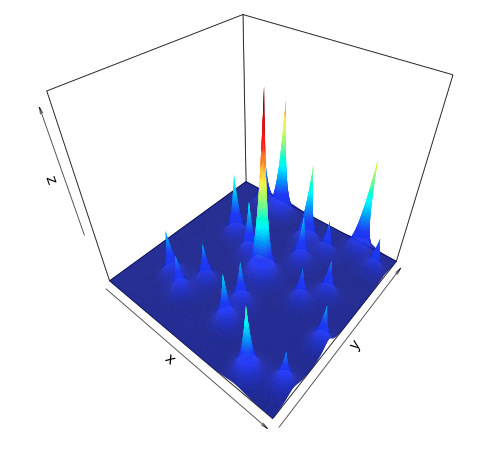
\includegraphics[width=0.4\textwidth]{Figures/Scaling/example_exp_mixture}
\caption[Synthetic density distribution]{Example of a synthetic density distribution obtained with the exponential mixture, with a grid of size $400\times 400$ and parameters $N=20$, $r_0=10$, $P_{max}=200$, $\alpha=0.5$, $\theta_C = 0.01$.}{}
\label{fig:ex-distrib}
\end{figure}
%%%%%%%%%%%%%%%%%%



%\begin{figure}
%\centering
%
%\caption{Validation of theoretical result through numerical simulation.}
%\label{fig:th_results}
%\end{figure}



\paragraph{Random Perturbations}{Perturbations aléatoires}

The simple model used is quite reducing for maximal densities and radius distribution. We aim to proceed to an empirical study of the influence of noise in the system by fixing $d_i^0$ and $r_i$ the following way :
\begin{itemize}
\item $d_i^0$ follows a reversed log-normal distribution with maximal value being a realistic maximal density
\item Radiuses are computed to respect rank-size law and then perturbed by a white noise. \comment{(Florent)  pourquoi ?}
\end{itemize}

%Results shown in Fig.~\ref{fig:random-density} are quantitatively different from previous one, as expected, but the same qualitative behavior is reproduced.


%\begin{figure}
%\centering

%\caption{Variation of exponents with variable origin density and radius.}
%\label{fig:random-density}
%\end{figure}



\paragraph{Kernel Type}{Type de Noyau}

We shall test the influence of the type of spatial kernel used on results. We can test gaussian kernels and quadratic kernels with parameters within reasonable ranges analog to the exponential kernel. %As shown in Fig.~\ref{fig:other-kernels}, we obtain the same qualitative results that is the significant variation of $\alpha(\theta)$ as a function of $\theta$.


%
%\begin{figure}
%\centering

%\caption{Scaling exponents for other kernels.}
%\label{fig:other-kernels}
%\end{figure}

%\paragraph{Two-parameters phase diagram}

%We introduce now a second spatial variable that has also an influence on the definition of urban entities, that is the proportion of actives working in city center, as done on empirical data in~\cite{cottineau2015scaling}. To simplify, it is used only to define urban parameter but assumed as having no influence on the local probability distribution of the amenity which stays the same function of the density. We write 

%\begin{figure}
%\centering

%\caption{Two parameters phase diagram.}
%\label{fig:two-params}
%\end{figure}

%%%%%%%%%%%%%%%%%%%%
%\subsection{Discussion}

%%%%%%%%%%%%%%%%%%%%
%\subsection{Conclusion}














%% Models behavior and refined exploration



\section{Model Explorations}{Exploration des Modèles} % Chapter title


This appendix gathers more precise model explorations, generally needed to support conclusions in main text but too long or repetitive to be included.


% Q : model behavior to be put in the thesis or in metadata link to git repo ?
%  -> as code, unreadable directly : put listing of statistical analysis
% TODO : find a way to automatically generate stat anal files from R ?







%%%%%%%%%%%%%%%%%%%%%%%
\section{Causalities in RBD model}{Causalités dans le modèle RBD}



%%%%%%%%%%%%%%%
\begin{figure}
%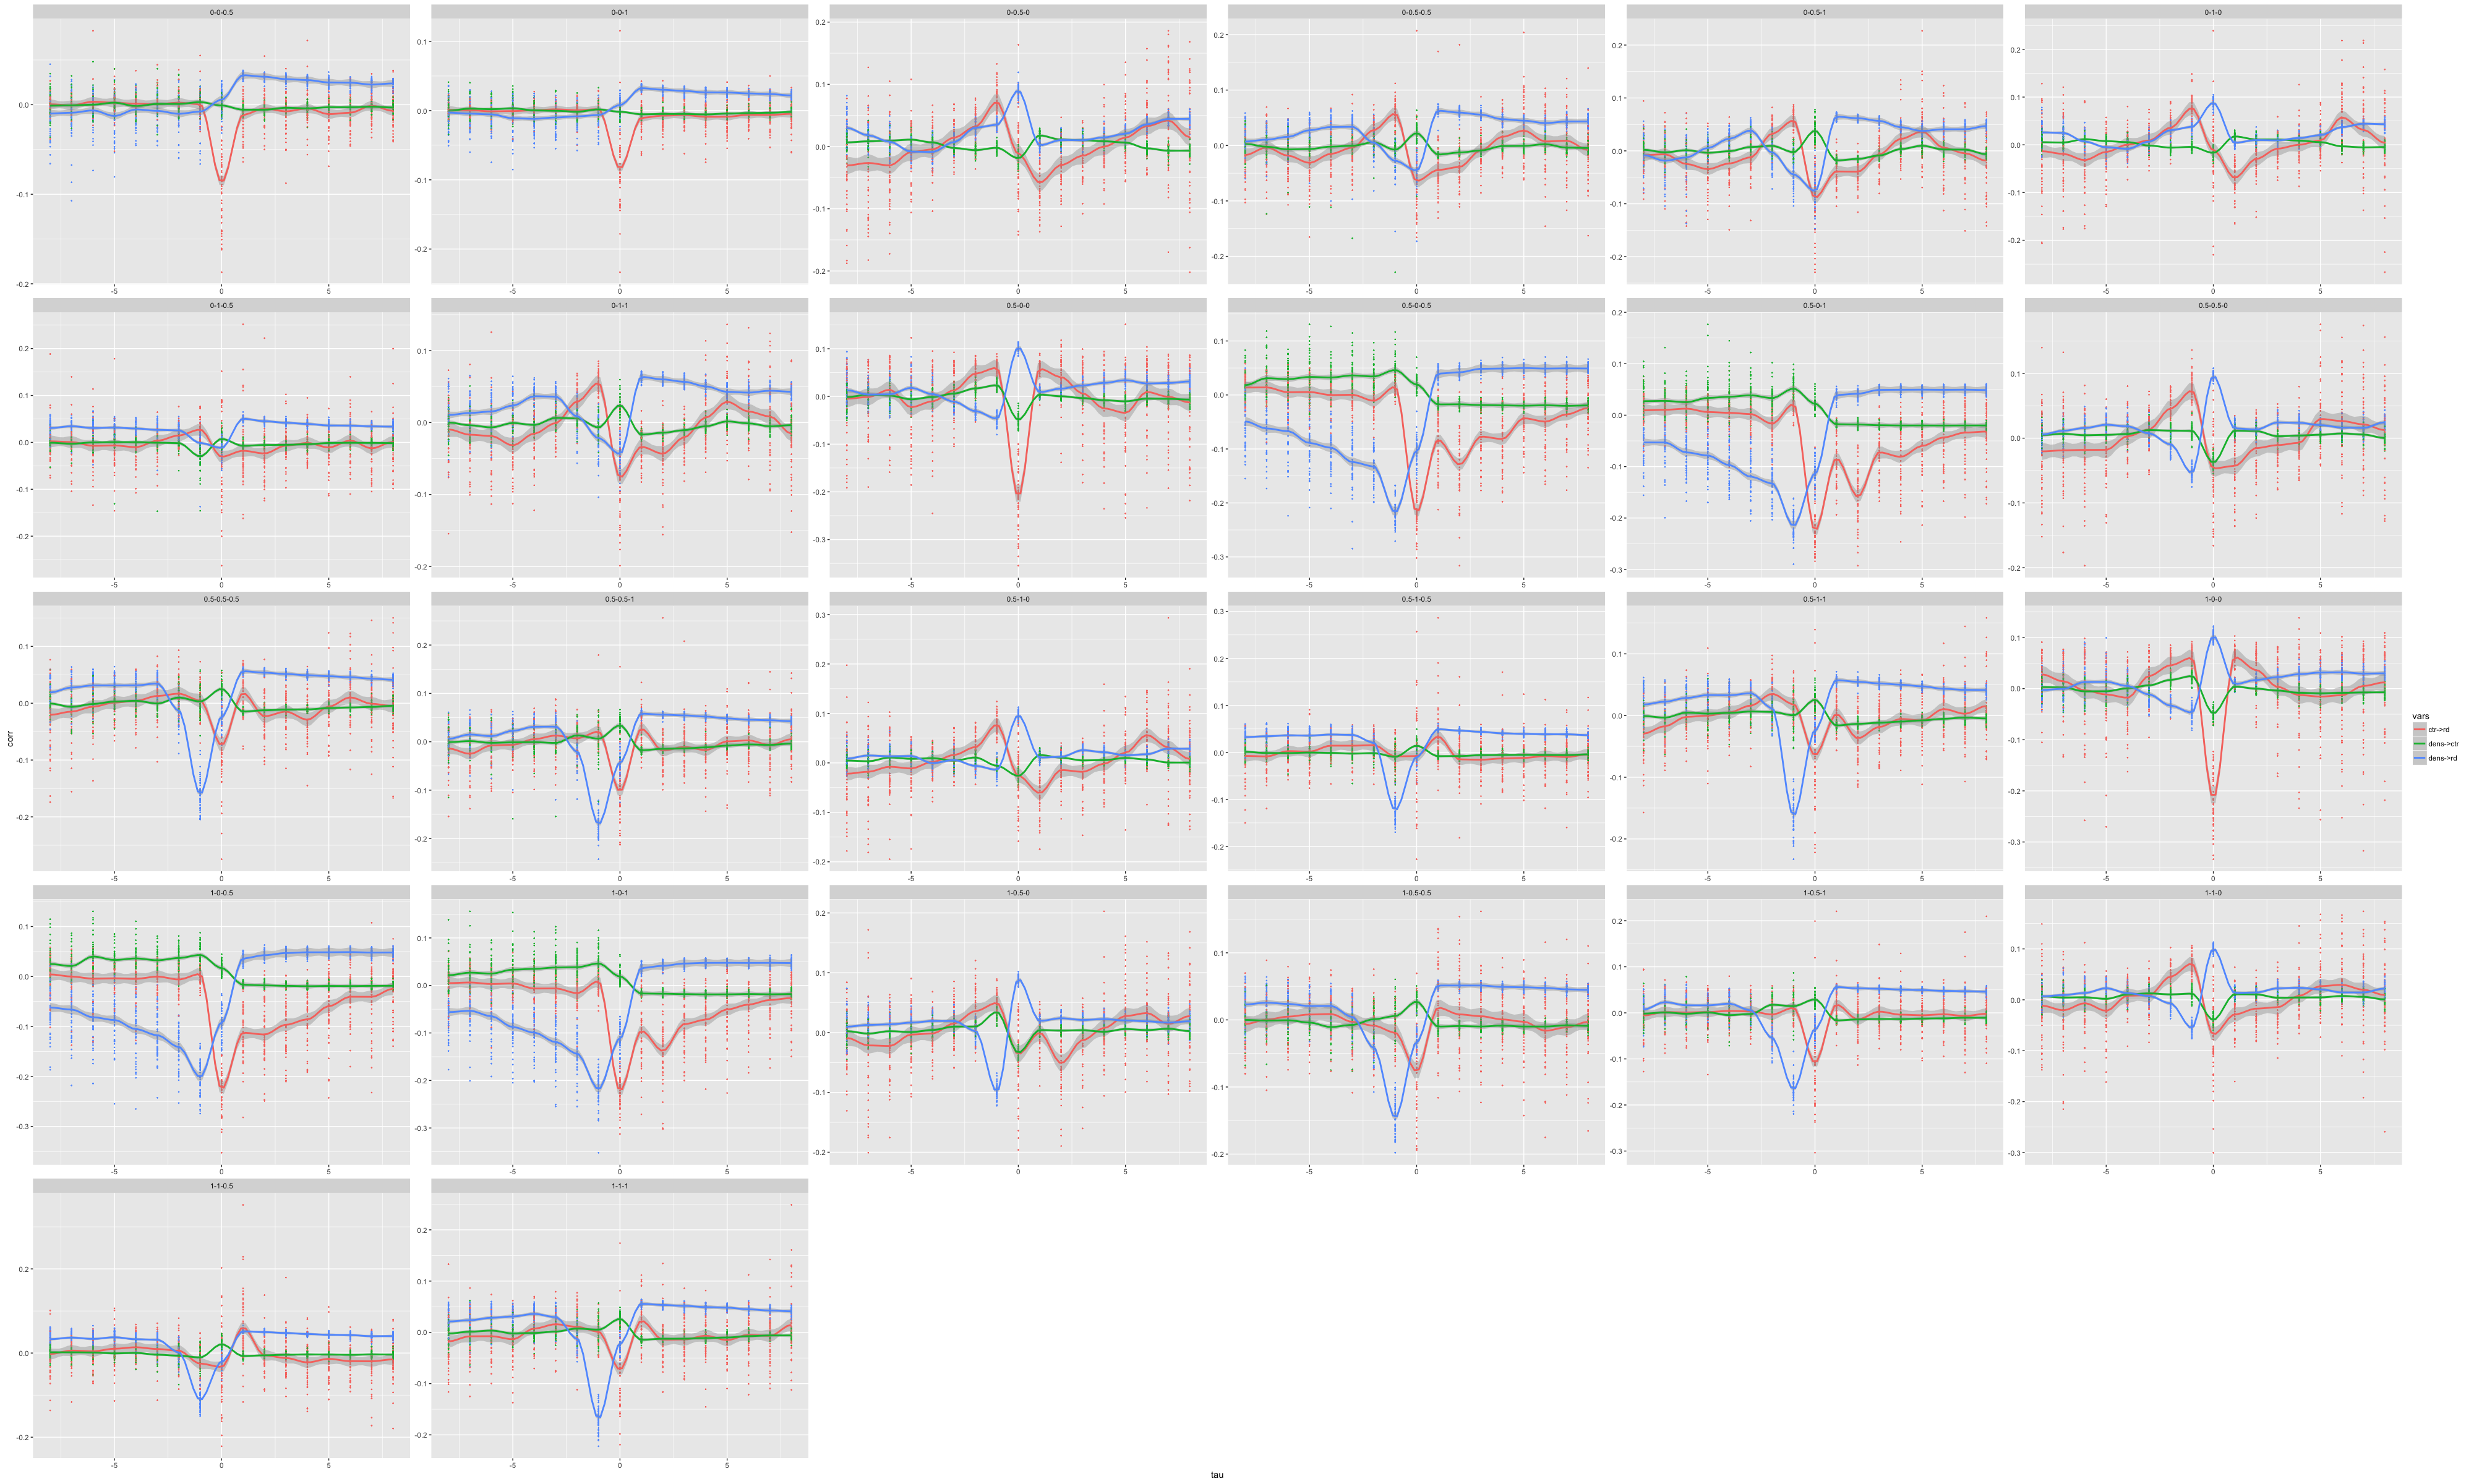
\includegraphics[height=\textwidth,angle=90]{Figures/SynthRBD/laggedcorrs_facet.png}
\caption[][]{}{}
\end{figure}
%%%%%%%%%%%%%%%





%%%%%%%%%%%%%%%%%%





%%%%%%%%%%%%%%%%%%%%%%%%%%%%%
% Appendix B (11) : Methodology
% Robustness Discrepancy

\newpage

%\section[A Discrepancy-based Framework][Un Cadre basé sur la Discrépance]{A Discrepancy-based Framework to Compare Robustness between Multi-Attribute Evaluations}{Un Cadre basé sur la Discrépance pour Comparer la Robustesse des Evaluations Multi-attributs} 
\section{A Discrepancy-based Framework}{Robustesse d'une évaluation multi-attributs}


\label{app:sec:robustness}


%----------------------------------------------------------------------------------------




\stars



\textit{Cette section a été publiée en anglais comme~\cite{raimbault2017discrepancy}. Elle est ici traduite et adaptée.}


\stars


\bpar{
Multi-objective evaluation is a necessary aspect when managing complex systems, as the intrinsic complexity of a system is generally closely linked to the potential number of optimization objectives. However, an evaluation makes no sense without its robustness being given (in the sense of its reliability). Statistical robustness computation methods are highly dependent of underlying statistical models. We propose a formulation of a model-independent framework in the case of integrated aggregated indicators (multi-attribute evaluation), that allows to define a relative measure of robustness taking into account data structure and indicator values. We implement and apply it to a synthetic case of urban systems based on Paris districts geography, and to real data for evaluation of income segregation for Greater Paris metropolitan area. First numerical results show the potentialities of this new method. Furthermore, its relative independence to system type and model may position it as an alternative to classical statistical robustness methods.
}{
Les évaluations multi-objectifs sont un aspect essentiel de la gestion de systèmes complexes, puisque la complexité intrinsèque d'un système est généralement étroitement liée au nombre d'objectifs d'optimisation potentiels. Cependant, une évaluation ne fait pas sens si sa robustesse, au sens de sa fiabilité, n'est pas donnée. Les méthodes statistiques usuelles fournissant une mesure de robustesse sont très dépendantes des modèles sous-jacents. Nous proposons une formulation d'un cadre indépendant du modèle, dans le cas d'indicateurs intégrés et agrégés (évaluation multi-attributs), qui permet de définir une mesure de robustesse relative prenant en compte la structure des données et les valeurs des indicateurs. La méthode est testée sur données urbaines synthétiques associées aux arrondissements de Paris, et à des données réelles de revenus pour l'évaluation de la ségrégation urbaine dans la région métropolitaine du Grand Paris. Les premiers résultats numériques montrent les potentialités de cette nouvelle méthode. De plus, sa relative indépendance au type de système et au modèle pourrait la positionner comme une alternative aux méthodes statistiques classiques d'évaluation de la robustesse.
}


%%%%%%%%%%%%%%%%
%% Intro
%%%%%%%%%%%%%%%%
\subsection{Introduction}{Introduction}

%%%%%%%%%%%%%%%%
\subsubsection{General Context}{Contexte Général}


\bpar{
Multi-objective problems are organically linked to the complexity of underlying systems. Indeed, either in the field of \emph{Complex Industrial Systems}, in the sense of engineered systems, where construction of Systems of Systems (SoS) by coupling and integration often leads to contradictory objectives~\cite{marler2004survey}, or in the field of \emph{Natural Complex Systems}, in the sense of non engineered physical, biological or social systems that exhibit emergence and self-organization properties, where objectives can e.g. be the result of heterogeneous interacting agents (see~\cite{newman2011complex} for a large survey of systems concerned by this approach), multi-objective optimization can be explicitly introduced to study or design the system but is often already implicitly ruling the internal mechanisms of the system. The case of socio-technical Complex Systems is particularly interesting as, following~\cite{haken2003face}, they can be seen as hybrid systems embedding social agents into ``technical artifacts'' (sometimes to an unexpected degree creating what \noun{Picon} describes as \emph{cyborgs}~\cite{picon2013smart}), and thus cumulate propensity to be at the origin of multi-objective issues\footnote{We design by \emph{Multi-Objective Evaluation} all practices including the computation of multiple indicators of a system (it can be multi-objective optimization for system design, multi-objective evaluation of an existing system, multi-attribute evaluation ; our particular framework corresponds to the last case).}. The new notion of \emph{eco-districts}~\cite{souami2012ecoquartiers} is a typical example where sustainability implies contradictory objectives. The example of transportation systems, which conception shifted during the second half of the 20th century from cost-benefit analysis to multi-criteria decision-making, is also typical of such systems~\cite{bavoux2005geographie}. Geographical system are now well studied from such a point of view in particular thanks to the integration of multi-objective frameworks within Geographical Information Systems~\cite{carver1991integrating}. As for the micro-case of eco-districts, meso and macro urban planning and design may be made sustainable through indicators evaluation~\cite{jegou2012evaluation}.
}{
Les problèmes multi-objectifs sont organiquement liés à la complexité des systèmes sous-jacents. En effet, que ce soit dans le champ des \emph{Systèmes Complexes Industriels}, dans le sens de systèmes conçus par ingénierie, où la construction de Systèmes de Systèmes (SoS) par couplage et intégration induit souvent des objectifs contradictoires~\cite{marler2004survey}, ou dans le champ des \emph{Systèmes Complexes Naturels}, au sens de systèmes non désignés, physiques, biologiques ou sociaux, qui présentent des propriétés d'émergence et d'auto-organisation, pour lesquels les objectifs peuvent e.g. être le résultat de l'interaction d'agents hétérogènes (voir~\cite{newman2011complex} pour une revue étendue des types de systèmes concernés par cette approche), l'optimisation multi-objectifs peut être explicitement introduite pour étudier ou désigner le système, mais régit généralement déjà implicitement les mécanismes internes du système. Le cas des Systèmes Complexes Sociaux-techniques est particulièrement intéressant puisque selon Haken~\cite{haken2003face}, ils peuvent être vus comme des systèmes hybrides embarquant des agents sociaux dans des ``artefacts techniques'' (parfois jusqu'à un niveau inattendu, créant ce que \noun{Picon} décrit comme \emph{cyborgs}~\cite{picon2013smart}), et cumulent ainsi la potentialité d'être à l'origine de problèmes multi-objectifs\footnote{Nous désignons ici par \emph{Evaluation Multi-objectifs} toutes les pratiques incluant le calcul de multiples indicateurs d'un système (il peut s'agir d'optimisation multi-objectif pour un design de système, une évaluation multi-objectif d'un système existant, une évaluation multi-attributs ; notre cadre particulier correspondra au dernier cas).}. La notion récente d'\emph{éco-quartier}~\cite{souami2012ecoquartiers} est un exemple typique pour lequel la durabilité implique des objectifs contradictoires. L'exemple des systèmes de transport, dont la conception a glissé durant la seconde moitié du 20ème siècle d'analyses coût-bénéfices à la price de décision multi-critères, est également typique de tels systèmes~\cite{bavoux2005geographie}. Les systèmes géographiques sont à présent bien étudiés d'un tel point de vue, en particulier grâce à l'intégration des cadres multi-objectifs au sein des Systèmes d'Information Géographiques~\cite{carver1991integrating}. Comme dans le cas microscopique des éco-quartiers, la planification et le design urbains mésoscopiques et macroscopiques peuvent être rendus durables grâce aux évaluations par indicateurs~\cite{jegou2012evaluation}.
}



\bpar{
A crucial aspect of an evaluation is a certain notion of its reliability, that we call here \emph{robustness}. % Various definitions of robustness are possible in different frames, and it will have a precise definition in our framework.
Statistics naturally include this notion since the construction and estimation of statistical models give diverse indicators of the consistence of results~\cite{launer2014robustness}. The first example that comes to mind is the application of the law of large numbers to obtain the \emph{p-value} of a model fit, that can be interpreted as a confidence measure of estimates. Besides, confidence intervals and \emph{beta-power} are other important indicators of statistical robustness. Bayesian inference provide also measures of robustness when distribution of parameters are sequentially estimated. Concerning multi-objective optimization, in particular through heuristic algorithms (for example genetic algorithms, or operational research solvers), the notion of robustness of a solution concerns more the stability of the solution on the phase space of the corresponding dynamical system. Recent progresses have been done towards unified formulation of robustness for a multi-objective optimization problem, such as~\cite{deb2006introducing} where robust Pareto-front as defined as solutions that are insensitive to small perturbations. In~\cite{1688537}, the notion of degree of robustness is introduced, formalized as a sort of continuity of other solutions in successive neighborhood of a solution.
}{
Un aspect crucial de l'évaluation est une certaine notion de sa fiabilité, que nous nommerons ici \emph{robustesse}. Les méthodes statistiques incluent naturellement cette notion puisque la construction et l'estimation de modèles statistiques donne divers indicateurs de la consistence des résultats~\cite{launer2014robustness}. Le premier exemple venant à l'esprit est l'application de la loi des grands nombres pour obtenir la \emph{p-valeur} d'une estimation de modèle, qui peut être interprété comme une mesure de confiance en les valeurs estimées. D'autre part, les intervalles de confiance et le  \emph{beta-power} sont d'autres indicateurs importants de robustesse statistique. L'inférence bayésienne fournit également des mesures de robustesse quand la distribution des paramètres est estimée de manière séquentielle. Concernant les optimisations multi-objectifs, en particulier par des algorithmes heuristiques (comme par exemple les algorithmes génétiques, ou les solveurs de recherche opérationelle), la notion de robustesse d'une solution consiste plus en la stabilité de la solution dans l'espace des phases du système dynamique correspondant. Des progrès récents ont été faits vers une formulation unifiée de la robustesse pour les problèmes d'optimisation multi-objectifs, comme dans~\cite{deb2006introducing} où les fronts de Pareto robustes sont définis comme des solutions insensibles aux petites perturbations. Dans~\cite{1688537}, la notion de degré de robustesse est introduite, formalisée comme une sorte de continuité des autres solutions dans des voisinages successifs d'une solution.
}


\bpar{
However, there still lack generic methods to estimate robustness of an evaluation that would be model-independent, i.e. that would be extracted from data structure and indicators but that would not depend on the method used. Some advantages could be for example an \emph{a priori} estimation of potential robustness of an evaluation and thus to decide if the evaluation is worth doing. We propose here a framework answering this issue in the particular case of Multi-attribute evaluations, i.e. when the problem is made unidimensional by objectives aggregation. It is data-driven and not model-driven in the sense that robustness estimation does not depend on how indicators are computed, as soon as they respect some assumptions that will be detailed in the following.
}{
Cependant, il n'existe pas de méthode générique qui permettrait une évaluation de la robustesse de façon indépendante au modèle, i.e. qui serait extraite de la structure des données et des indicateurs mais ne dépendrait pas de la méthode utilisée. Un avantage serait par exemple une estimation \emph{a priori} de la robustesse potentielle d'une évaluation et de décider ainsi si elle vaut la peine d'être faite. Nous proposons un cadre répondant à cette contrainte dans le cas particulier des évaluations multi-attributs, i.e. quand le problème est rendu unidimensionnel par agrégation des objectifs. Il est basé sur les données et non sur les modèles, au sens ou l'estimation de la robustesse ne dépendra pas de la manière dont les indicateurs sont calculés, tant qu'ils respectent certaines hypothèses détaillées par la suite.
}



%%%%%%%%%%%%%%%%
\subsubsection{Proposed Approach}{Approche Proposée}



\paragraph{Objectives as Spatial Integrals}{Objectifs comme intégrales spatiales}


\bpar{
We assume that objectives can be expressed as spatial integrals, so it should apply to any territorial system and our application cases are urban systems. It is not that restrictive in terms of possible indicators if one uses suitable variables and integrated kernels : in a way analog to the method of geographically weighted regression~\cite{brunsdon1998geographically}, any spatial variable can be integrated against regular kernels of variable size and the result will be a spatial aggregation which sense depends on kernel size. The example we use in the following such as conditional means or sums suit well the assumption. Even an already spatially aggregated indicator can be interpreted as a spatial indicator by using a Dirac distribution on the centroid of the corresponding area.
}{
Nous supposons que les objectifs peuvent être exprimés comme intégrales spatiales, ce qui devrait s'appliquer à tout système territorial, et nos cas d'application sont des systèmes urbains. Ce n'est pas si restrictif en terme d'indicateurs possibles si l'on utilise les bonnes variables et noyaux intégrés : de façon analogue à la méthode de Regression Géographique Pondérée~\cite{brunsdon1998geographically}, toute variable spatiale peut être intégrée contre des noyaux réguliers de taille variable et le résultats sera une agrégation spatiale dont la signification dépendra de l'étendue du noyau. Les exemples utilisés par la suite comme des moyennes conditionnelles ou des sommes vérifient parfaitement cette hypothèse. Même un indicateur déjà agrégé dans l'espace peut être interprété comme une intégrale spatiale en utilisant une distribution de Dirac au centroïde de la zone correspondante. 
}



\paragraph{Linearly Aggregated Objectives}{Objectifs agrégés linéairement}

\bpar{
A second assumption we make is that the multi-objective evaluation is done through linear aggregation of objectives, i.e. that we are tackling a multi-attribute optimization problem. If $(q_i(\vec{x}))_i$ are values of objectives functions, then weights $(w_i)_i$ are defined in order to build the aggregated decision-making function $q(\vec{x})=\sum_i{w_i q_i(\vec{x})}$, which value determines then the performance of the solution. It is analog to aggregated utility techniques in economics and is used in many fields. The subtlety lies in the choice of weights, i.e. the shape of the projection function, and various approaches have been developed to find weights depending on the nature of the problem. Recent work~\cite{dobbie2013robustness} proposed to compare robustness of different aggregation techniques through sensitivity analysis, performed by Monte-Carlo simulations on synthetic data. Distribution of biases where obtained for various techniques and some showed to perform significantly better than others. Robustness assessment still depended on models used in that work.
}{
Une seconde hypothèse que nous faisons est que l'évaluation multi-objectifs est effectuée par agrégation linéaire des objectif, c'est à dire qu'on se place dans le cadre d'un problème d'optimisation multi-attributs. Si $(q_i(\vec{x}))_i$ sont les valeurs des fonctions objectifs, on définit alors des poids $(w_i)_i$ afin de construire la fonction de prise de décision $q(\vec{x})=\sum_i{w_i q_i(\vec{x})}$, dont la valeur détermine ensuite la performance d'une solution. Cette approche est analogue aux utilités agrégées en économie et est utilisée dans de nombreux domaines. La subtilité réside dans le choix des poids, i.e. de la forme de la fonction de projection, et différentes solutions ont été dévelopées pour obtenir des poids selon la nature du problème. Récemment, \cite{dobbie2013robustness} a proposé de comparer la robustesse des différentes techniques d'agrégation par une analyse de sensibilité, effectuée par simulations de Monte-Carlo pour produire des données synthétiques, ce qui permet d'obtenir la distribution des biais pour les différentes techniques, certaines étant significativement plus performantes que d'autres. Toutefois, la quantification de la robustesse dépend toujours des modèles utilisés dans ce travail.
}


\bigskip


\bpar{
The rest of the paper is organized as follows : section 2 describes intuitively and mathematically the proposed framework ; section 3 then details implementation, data collection for case studies and numerical results for an artificial intra-urban case and a metropolitan real case ; section 4 finally discuss limitations and potentialities of the method.
}{
Le reste de cette monographie est organisé de la façon suivante : la section 2 décrit intuitivement puis mathématiquement le cadre proposé ; la section 3 détaille ensuite l'implémentation, la collecte des données pour les cas d'étude et les résultats numériques pour une évaluation intra-urbaine synthétique et un cas réel métropolitain ; la section 4 discute finalement les limitations et les potentialités de la méthode.
}




%%%%%%%%%%%%%%%%
%% Framework Description
%%%%%%%%%%%%%%%%
\subsection{Framework Description}{Description du Cadre}


%%%%%%%%%%%%%%%%
\subsubsection{Intuitive Description}{Description Intuitive}


\bpar{
We describe now the abstract framework allowing theoretically to compare robustnesses of evaluations of two different urban systems. Our framework is a generalization of an empirical method proposed in~\cite{ecodistrictReport} besides a more general benchmarking study on indicator sense and relevance in a sustainability context. Intuitively, it relies on empirical base resulting from the following axioms :
\begin{itemize}
\item Urban systems can be seen from the information available, i.e. raw data describing the system. As a data-driven approach, this raw data is the basis of our framework and robustness will be determined by its structure.
\item From data are computed indicators (objective functions). We assume that a choice of indicators is an intention to translate particular aspects of the system, i.e. to capture a realization of an ``urban fact'' (\emph{fait urbain}) in the sense of \noun{Mangin}~\cite{mangin1999projet} - a sort of stylized fact in terms of processes and mechanisms, having various realizations on spatially distinct systems, depending on each precise context.
\item Given many systems and associated indicators, a common space can be built to compare them. In that space, data represents more or less well real systems, depending e.g. on initial scale, precision of data, missing data. We precisely propose to capture that through the notion of point cloud discrepancy, which is a mathematical tool coming from sampling theory expressing how a dataset is distributed in the space it is embedded in~\cite{dick2010digital}. %Coupling discrepancies with appropriate weights depending on indicator importance allows to introduce a relative ratio of robustness between two evaluations.
\end{itemize}


Synthesizing these requirements, we propose a notion of \emph{Robustness} of an evaluation that captures both, by combining data reliability with relative importance,
\begin{enumerate}
\item \emph{Missing Data} : an evaluation based on more refined datasets will naturally be more robust.
\item \emph{Indicator importance} : indicators with more relative influence will weight more on the total robustness.
\end{enumerate}
}{
Nous décrivons à présent le cadre proposé pour permettre théoriquement de comparer la robustesse d'évaluation de deux systèmes urbains différents. Ce cadre est une généralisation d'une méthode empirique proposée dans~\cite{ecodistrictReport} pour accompagner une étude dans un autre contexte effectuant une comparaison du sens et de la pertinence des indicateurs dans un contexte de durabilité. Intuitivement, la base empirique se base sur les principes suivants :

\begin{itemize}
\item Les systèmes urbains peuvent être vus selon l'information disponible, i.e. les données brutes décrivant le système. Dans une approche basée sur les données, celles-ci sont la base de notre cadre et la robustesse sera déterminée par leur structure.
\item A partir des données sont capturés des indicateurs (fonctions objectifs). Nous supposons qu'un choix d'indicateurs est une intention particulière de traduire des aspects particuliers du système, i.e. de capturer une réalisation d'un ``fait urbain'' au sens de \noun{Mangin}~\cite{mangin1999projet} - une sorte de fait stylisé en terme de processus et de mécanismes, ayant différentes réalisations sur des systèmes distincts dans l'espace, dépendant de chaque contexte géographique précis.
\item Etant donné plusieurs systèmes et indicateurs associés, un espace commun peut être construit pour les comparer. Dans cet espace, les données représentent plus ou moins bien le système réel, c'est à dire qu'elles sont imprécises en fonction de l'échelle initiale, de la précision effective des données. Nous proposons de capturer exactement ces différents aspects au travers de la notion de discrépance d'un nuage de points, qui est un outil mathématique provenant des théories d'échantillonnage, permettant d'exprimer la façon dont un jeu de données rempli l'espace dans lequel il s'insère~\cite{dick2010digital}.
\end{itemize}

Synthétisant ces contraintes, nous proposons une notion de \emph{Robustesse} d'une évaluation qui capture à la fois, en combinant la fiabilité des données à l'importance relative des indicateurs,


\begin{enumerate}
\item \emph{Données manquantes} : une évaluation se basant sur des jeux de données plus raffinés sera naturellement plus robuste.
\item \emph{Importance des indicateurs} : les indicateurs avec plus d'importance relative pèseront plus dans la robustesse totale.
\end{enumerate}
}




%%%%%%%%%%%%%%%%
\subsubsection{Formal Description}{Description Formelle}


%%%%%%%%%%%%%%%%
\paragraph{Indicators}{Indicateurs}


\bpar{
Let $(S_{i})_{1\leq i\leq N}$ be a finite number of geographically disjoints territorial systems, that we assume described through raw data and intermediate indicators, yielding $S_{i}=(\mathbf{X}_{i},\mathbf{Y}_{i})\in\mathcal{X}_{i}\times\mathcal{Y}_{i}$ with $\mathcal{X}_{i}=\prod_{k}\mathcal{X}_{i,k}$ such that each subspace contain real matrices : $\mathcal{X}_{i,k}=\mathbb{R}^{n_{i,k}^{X}p_{i,k}^{X}}$ (the same holding for $\mathcal{Y}_{i}$). We also define an ontological index function $I_{X}(i,k)$ (resp. $I_{Y}(i,k)$) taking integer values which coincide if and only if the two variables have the same ontology in the sense of~\cite{livet2010}, i.e. they are supposed to represent the same real object. We distinguish ``raw data'' $\mathbf{X}_{i}$ from which indicators are computed via explicit deterministic functions, from ``intermediate indicators'' $\mathbf{Y}_{i}$ that are already integrated and can be e.g. outputs of elaborated models simulating some aspects of the urban system. We define the partial characteristic space of the ``urban fact'' by 

\begin{equation}
%\begin{split}
%(\mathcal{X},\mathcal{Y}) & \underset{def}{=} \left(\prod\tilde{\mathcal{X}}_{c}\right)\times\left(\prod\tilde{\mathcal{Y}}_{c}\right)\\
%& =  \left(\prod_{\mathcal{X}_{i,k}\in\mathcal{D}_{\mathcal{X}}}\mathbb{R}^{p_{i,k}^{X}}\right)\times\left(\prod_{\mathcal{Y}_{i,k}\in\mathcal{D}_{\mathcal{Y}}}\mathbb{R}^{p_{i,k}^{Y}}\right)
%\end{split}
(\mathcal{X},\mathcal{Y}) \underset{def}{=} \left(\prod\tilde{\mathcal{X}}_{c}\right)\times\left(\prod\tilde{\mathcal{Y}}_{c}\right) = \left(\prod_{\mathcal{X}_{i,k}\in\mathcal{D}_{\mathcal{X}}}\mathbb{R}^{p_{i,k}^{X}}\right)\times\left(\prod_{\mathcal{Y}_{i,k}\in\mathcal{D}_{\mathcal{Y}}}\mathbb{R}^{p_{i,k}^{Y}}\right)
\end{equation}


with $\mathcal{D}_{\mathcal{X}}=\{\mathcal{X}_{i,k}|I(i,k)\textrm{ distincts},n_{i,k}^{X}\mbox{ maximal}\}$
(the same holding for $\mathcal{Y}_{i}$). It is indeed the abstract space on which indicators are integrated. The indices $c$ introduced as a definition here correspond to different indicators across all systems. This space is the minimal space common to all systems allowing a common definition for indicators on each.
}{
Soit $(S_{i})_{1\leq i\leq N}$ un nombre fini de systèmes territoriaux géographiquement disjoints, \comment{Q pourquoi nécessaire des les avoir spatially disjoints, could be different indicators on the same area ? maybe makes less sense ? missing point for comparability ?}
que nous supposons décrits par les données brutes et des indicateurs intermédiaires, donnés par $S_{i}=(\mathbf{X}_{i},\mathbf{Y}_{i})\in\mathcal{X}_{i}\times\mathcal{Y}_{i}$ avec $\mathcal{X}_{i}=\prod_{k}\mathcal{X}_{i,k}$ tel que chaque sous-espace contient des matrices réelles : $\mathcal{X}_{i,k}=\mathbb{R}^{n_{i,k}^{X}p_{i,k}^{X}}$ (de la même façon pour $\mathcal{Y}_{i}$). Nous définissons également une fonction d'indice ontologique $I_{X}(i,k)$ (resp. $I_{Y}(i,k)$) prenant des valeurs entières qui coincident si et seulement si les deux variables ont même ontologie au sens de~\cite{livet2010}, c'est à dire qu'elles sont supposées représenter le même objet réel. On distingue les ``données brutes'' $\mathbf{X}_{i}$ à partir desquelles les indicateurs sont calculés généralement par des fonctions déterministes explicites, \comment{not that free on the computation here !}
 des ``indicateurs intermédiaires'' $\mathbf{Y}_{i}$ qui sont déjà intégrés et peuvent être par exemple les sorties de modèles élaborés simulant certains aspects du système urbain. Nous définissons l'espace caractéristique du ``fait urbain'' par


\begin{equation}
(\mathcal{X},\mathcal{Y}) \underset{def}{=} \left(\prod\tilde{\mathcal{X}}_{c}\right)\times\left(\prod\tilde{\mathcal{Y}}_{c}\right) = \left(\prod_{\mathcal{X}_{i,k}\in\mathcal{D}_{\mathcal{X}}}\mathbb{R}^{p_{i,k}^{X}}\right)\times\left(\prod_{\mathcal{Y}_{i,k}\in\mathcal{D}_{\mathcal{Y}}}\mathbb{R}^{p_{i,k}^{Y}}\right)
\end{equation}

avec $\mathcal{D}_{\mathcal{X}}=\{\mathcal{X}_{i,k}|I(i,k)\textrm{ distincts},n_{i,k}^{X}\mbox{ maximal}\}$
(de même pour $\mathcal{Y}_{i}$). Il s'agit en fait de l'espace abstrait sur lequel les indicateurs sont intégrés. Les indices $c$ introduit par définition correspondent aux différents indicateurs au sein des différents systèmes. Cette espace est l'espace minimal commun à tous les systèmes permettant une définition commune des indicateurs pour tous.
}



\bpar{
Let $\mathbf{X}_{i,c}$ be the data canonically projected in the corresponding subspace, well defined for all $i$ and all $c$. We make the key assumption that all indicators are computed by integration against a certain kernel, i.e. that for all $c$, there exists $H_{c}$ space of real-valued functions on $(\tilde{\mathcal{X}}_{c},\tilde{\mathcal{Y}}_{c})$, such that for all $h\in H_{c}$ :
\begin{enumerate}
\item $h$ is ``enough'' regular (tempered distributions e.g.)
\item $q_c=\int_{(\tilde{\mathcal{X}}_{c},\tilde{\mathcal{Y}}_{c})}h$ is a function describing the ``urban fact'' (the indicator in itself)
\end{enumerate}

Typical concrete example of kernels can be :

\begin{itemize}
\item A mean of rows of $\mathbf{X}_{i,c}$ is computed with $h(x)=x\cdot f_{i,c}(x)$ where $f_{i,c}$ is the density of the distribution of the assumed underlying variable.
\item A rate of elements respecting a given condition $C$, $h(x)=f_{i,c}(x)\chi_{C(x)}$ 
\item For already aggregated variables $\mathbf{Y}$, a Dirac distribution allows to express them also as a kernel integral. 
\end{itemize}
}{
Soit $\mathbf{X}_{i,c}$ les données projetées canoniquement sur le sous-espace correspondant, bien définies pour tout $i$ et tout $c$. Nous faisons donc l'hypothèse clé que tous les indicateurs sont calculés par intégration contre un noyau donné, i.e. pour tout $c$ il existe $H_{c}$ espace de fonctions à valeurs réelles sur $(\tilde{\mathcal{X}}_{c},\tilde{\mathcal{Y}}_{c})$, tel que pour tout $h\in H_{c}$ : 

\begin{enumerate}
\item $h$ est ``suffisamment'' régulière (distribution tempérée par exemple)
\item $q_c=\int_{(\tilde{\mathcal{X}}_{c},\tilde{\mathcal{Y}}_{c})}h$ est une fonction décrivant le ``fait urbain'' (l'indicateur en lui-même)
\end{enumerate}

Des exemples typiques de noyaux peuvent être :


\begin{itemize}
\item Une moyenne des lignes de $\mathbf{X}_{i,c}$ est calculée par $h(x)=x\cdot f_{i,c}(x)$ où $f_{i,c}$ est la densité de la distribution de la variable sous-jacente.
\item Un taux d'éléments du jeu de données respectant une condition donnée $C$, $h(x)=f_{i,c}(x)\chi_{C(x)}$.
\item Pour des variables déjà agrégées $\mathbf{Y}$, une distribution de Dirac permet des les exprimer également comme des intégrales de noyaux.
\end{itemize}

}


%%%%%%%%%%%%%%%%
\paragraph{Aggregation}{Agrégation}


\bpar{
Weighting objectives in multi-attribute decision-making is indeed the crucial point of the processes, and numerous methods are available (see~\cite{wang2009review} for a review for the particular case of sustainable energy management). Let define weights for the linear aggregation. We assume the indicators normalized, i.e. $q_c \in [0,1]$, for a more simple construction of relative weights. For $i,c$ and $h_{c}\in H_{c}$ given, the weight $w_{i,c}$ is simply constituted by the relative importance of the indicator $w_{i,c}^{L}=\frac{\hat{q}_{i,c}}{\sum_{c}\hat{q}_{i,c}}$ where $\hat{q}_{i,c}$ is an estimator of $q_{c}$ for data $\mathbf{X}_{i,c}$ (i.e. the effectively calculated value). Note that this step can be extended to any sets of weight attributions, by taking for example $\tilde{w}_{i,c} = w_{i,c} \cdot w'_{i,c}$ if $\mathbf{w}'$ are the weights attributed by the decision-maker. We focus here on the relative influence of attributes and thus choose this simple form for weights.
}{
La détermination des poids est en fait le point crucial des processus de prise de décision multi-attributs, et de nombreuses méthodes sont disponibles (voir~\cite{wang2009review} pour une revue dans le cas particulier de la gestion de l'énergie durable). Définissons les poids pour l'agrégation linéaire. Nous supposons les indicateurs normalisés, i.e. $q_c \in [0,1]$, pour une construction plus simple des poids relatifs. \comment{indeed $h_c \in [0,1]$ is the right assumption}
Pour $i,c$ et $h_{c}\in H_{c}$ donnés, le poids $w_{i,c}$ est simplement constitué par l'importance relative de l'indicateur $w_{i,c}^{L}=\frac{\hat{q}_{i,c}}{\sum_{c}\hat{q}_{i,c}}$ où $\hat{q}_{i,c}$ est un estimateur de $q_{c}$ pour les données $\mathbf{X}_{i,c}$ (i.e. la valeur calculée effectivement). On peut noter que cette étape n'est pas contraignante et que cela peut être étendu à tout ensemble d'attribution de poids, en prenant par exemple $\tilde{w}_{i,c} = w_{i,c} \cdot w'_{i,c}$ si $\mathbf{w}'$ sont les poids fixés par le preneur de décisions. Nous nous concentrons sur l'influence relative des attributs et pour cela choisissons cette forme simple pour les poids. 
}










%%%%%%%%%%%%%%%%
\paragraph{Robustness Estimation}{Estimation de la Robustesse}


\bpar{
The scene is now set up to be able to estimate the robustness of the evaluation done through the aggregated function. Therefore, we apply an integral approximation method similar to methods introduced in~\cite{varet2010developpement}, since the integrated form of indicators indeed brings the benefits of such powerful theoretical results. Let $\mathbf{X}_{i,c}=(\vec{X}_{i,c,l})_{1\leq l\leq n_{i,c}}$ and $D_{i,c}=Disc_{\tilde{\mathcal{X}}_{c},L^2}(\mathbf{X}_{i,c})$ the discrepancy of data points cloud\footnote{The discrepancy is defined as the $L2$-norm of local discrepancy which is for normalized data points $\mathbf{X}=(x_{ij})\in \left[0,1\right]^d$, a function of $\mathbf{t}\in \left[0,1\right]^d$ comparing the number of points falling in the corresponding hypercube with its volume, by $disc(\mathbf{t}) = \frac{1}{n}\sum_i \mathbbm{1}_{\prod_j x_{ij}<t_j} - \prod_j t_j$. It is a measure of how the point cloud covers the space.}~\cite{niederreiter1972discrepancy}. With $h\in H_{c}$, we have the upper bound on the integral approximation error

\[
\left\Vert \int h_{c}-\frac{1}{n_{i,c}}\sum_{l}h_{c}(\vec{X}_{i,c,l})\right\Vert \leq K\cdot\left|\left|\left|h_{c}\right|\right|\right|\cdot D_{i,c}
\]

where $K$ is a constant independent of data points and objective function. It directly yields

\[
\left\Vert \int\sum w_{i,c}h_{c}-\frac{1}{n_{i,c}}\sum_{l}w_{i,c}h_{c}(\vec{X}_{i,c,l})\right\Vert \leq K\sum_{c}\left|w_{i,c}\right|\left|\left|\left|h_{c}\right|\right|\right|\cdot D_{i,c}
\]

Assuming the error reasonably realized (``worst case'' scenario for knowledge of the theoretical value of aggregated function), we take this upper bound as an approximation of its magnitude. Furthermore, taking normalized indicators implies $\left|\left|\left|h_c\right|\right|\right| = 1$. We propose then to compare error bounds between two evaluations. They depend only on data distribution (equivalent to \emph{statistical robustness}) and on indicators chosen (sort of \emph{ontological robustness}, i.e. do the indicators have a real sense in the chosen context and do their values make sense), and are a way to combine these two type of robustnesses into a single value.
}{
La scène est à présent apprêtée pour construire une estimation de la robustesse d'une évaluation faite par la fonction d'agrégation. Pour cela, nous appliquons un théorème d'approximation d'intégrale similaire au méthodes introduites dans~\cite{varet2010developpement}, puisque la forme intégrée des indicateurs permet justement de bénéficier de tels résultats théoriquement puissant. Soit $\mathbf{X}_{i,c}=(\vec{X}_{i,c,l})_{1\leq l\leq n_{i,c}}$ et $D_{i,c}=Disc_{\tilde{\mathcal{X}}_{c},L^2}(\mathbf{X}_{i,c})$ le discrépance du jeu de données\footnote{La discrépance est définie comme la norme-$L2$ de la discrépance locale qui est pour des points de données normalisés $\mathbf{X}=(x_{ij})\in \left[0,1\right]^d$, une fonction de $\mathbf{t}\in \left[0,1\right]^d$ comparant le nombre de points compris dans le volume de l'hypercube correspondant, donné par $disc(\mathbf{t}) = \frac{1}{n}\sum_i \mathbbm{1}_{\prod_j x_{ij}<t_j} - \prod_j t_j$. C'est une mesure de la manière dont le nuage de points couvre l'espace.}~\cite{niederreiter1972discrepancy}. Avec $h\in H_{c}$, on a la borne supérieure sur l'erreur d'approximation de l'intégrale

\[
\left\Vert \int h_{c}-\frac{1}{n_{i,c}}\sum_{l}h_{c}(\vec{X}_{i,c,l})\right\Vert \leq K\cdot\left|\left|\left|h_{c}\right|\right|\right|\cdot D_{i,c}
\]

où $K$ est une constante indépendante des points de données et des fonctions objectifs. Cela donne directement

\[
\left\Vert \int\sum w_{i,c}h_{c}-\frac{1}{n_{i,c}}\sum_{l}w_{i,c}h_{c}(\vec{X}_{i,c,l})\right\Vert \leq K\sum_{c}\left|w_{i,c}\right|\left|\left|\left|h_{c}\right|\right|\right|\cdot D_{i,c}
\]


En supposant l'erreur réalisée de manière raisonnable (scénario du ``pire de cas'' pour la connaissance de la valeur théorique de la fonction agrégée), nous prenons cette borne supérieure comme une approximation de sa magnitude. De plus, la normalisation des indicateurs implique que $\left|\left|\left|h_c\right|\right|\right| = 1$. Nous proposons alors de comparer les bornes d'erreurs entre deux évaluations. Elle dépendent seulement de la distribution des données (équivalence à la \emph{robustesse statistique}) et des indicateurs choisis (sorte de \emph{robustesse ontologique}, i.e. est-ce que les indicateurs ont un sens réel dans le contexte choisi et est-ce que leur valeur fait sens), et sont un moyen de combiner ces deux types de robustesse dans une seule valeur.

}


\bpar{
We thus define a \emph{robustness ratio} to compare the robustness of two evaluations by
}{
Nous définissons ainsi un \emph{ratio de robustesse} pour comparer la robustesse de deux évaluations par 
}

\begin{equation}
R_{i,i'}=\frac{\sum_{c}w_{i,c}\cdot D_{i,c}}{\sum_{c}w_{i',c}\cdot D_{i',c}}
\end{equation}

\bpar{
The intuitive sense of this definition is that one compares robustness of evaluations by comparing the highest error done in each based on data structure and relative importance.
}{
L'interprétation intuitive de cette définition est que l'on compare la robustesse des évaluations en comparant la plus grande erreur faite dans chaque cas selon la structure des données et l'importance relative.
}



\bpar{
By taking then an order relation on evaluations by comparing the position of the ratio to one, it is obvious that we obtain a complete order on all possible evaluations. This ratio should theoretically allow to compare any evaluation of an urban system. To keep an ontological sense to it, it should be used to compare disjoints sub-systems with a reasonable proportion of indicators in common, or the same sub-system with varying indicators. Note that it provides a way to test the influence of indicators on an evaluation by analyzing the sensitivity if the ratio to their removal. On the contrary, finding a ``minimal'' number of indicators each making the ratio strongly vary should be a way to isolate essential parameters ruling the sub-system.
}{
En construisant une relation d'ordre sur les évaluations en comparant la position du ratio par rapport à un, il est clair qu'on obtient un ordre complet sur l'ensemble des évaluations possibles. Ce ratio devrait en théorie permettre de comparer n'importe quelle évaluation d'un système urbain. Afin de garder un sens ontologique à cela, il devrait être utilisé pour comparer des sous-systèmes disjoints  avec une proportion raisonnable d'indicateurs en commun, ou le même sous-système avec des indicateurs différents. On peut noter que cela fournit un moyen de tester l'influence des indicateurs sur une évaluation, en analysant la sensibilité du ratio à leur suppression. Au contraire, la détermination d'un nombre ``minimal'' d'indicateurs faisant chacun varier le ratio fortement pourrait être un moyen d'isoler des paramètres essentiels régissant le sous-système.
}





%%%%%%%%%%%%%%%%
%% Results
%%%%%%%%%%%%%%%%
\subsection{Results}{Résultats}

%We apply our framework to a ``toy-model'', as elaborated indicator definition nor raw data collection was not the primary aim of this work, which was more to theoretically introduce the framework. It is however essential for such a data-driven paradigm to demonstrate through simulation the potentialities of the method, what we do here on semi-synthetic data.


%%%%%%%%%%%%%%%%
\paragraph{Implementation}{Implémentation}


\bpar{
Preprocessing of geographical data is made through QGIS~\cite{qgis2011quantum} for performance reasons. Core implementation of the framework is done in R~\cite{team2000r} for the flexibility of data management and statistical computations. Furthermore, the package \texttt{DiceDesign}~\cite{franco20092} written for numerical experiments and sampling purposes, allows an efficient and direct computation of discrepancies. Last but not least, all source code is openly available on the \texttt{git} repository of the project\footnote{at \url{https://github.com/JusteRaimbault/RobustnessDiscrepancy}} for reproducibility purposes~\cite{ram2013git}.
}{
Le pré-traitement des données géographiques est fait via QGIS~\cite{qgis2011quantum} pour des raisons de performances.\comment{plutôt ergonomie ?}
L'implémentation du coeur est faite en R~\cite{team2000r} pour la flexibilité de la gestion des données et du traitement statistique. De plus, le package \texttt{DiceDesign}~\cite{franco20092} conçu pour les expériences numériques et l'échantillonnage, permet un calcul efficient et direct des discrépances. Enfin, tout aussi important, l'ensemble du code source est disponible de manière ouverte sur le dépôt \texttt{git}du projet\footnote{à \url{https://github.com/JusteRaimbault/RobustnessDiscrepancy}} pour permettre la reproductibilité et la réutilisation~\cite{ram2013git}.
}



%%%%%%%%%%%%%%%%
\subsubsection{Implementation on Synthetic Data}{Implémentation sur Données Synthétiques}


\bpar{
We propose in a first time to illustrate the implementation with an application to synthetic data and indicators, for intra-urban quality indicators in the city of Paris.
}{
Nous proposons dans un premier temps d'illustrer l'implémentation par une application à des données et indicateurs synthétiques, pour des indicateurs de qualité de vie intra-urbaine pour la ville de Paris.
}


%%%%%%%%%%%%%%%%
\paragraph{Data Collection}{Collecte des données}

\bpar{
We base our virtual case on real geographical data, in particular for \emph{arrondissements} of Paris. We use open data available through the OpenStreetMap project~\cite{bennett2010openstreetmap} that provides accurate high definition data for many urban features. We use the street network and position of buildings within the city of Paris. %\footnote{for which the third-party website \url{https://mapzen.com/metro-extracts/} provides already packaged extracts as for many metropolitan areas of the world}
Limits of \emph{arrondissements}, used to overlay and extract features when working on single districts, are also extracted from the same source. We use centroids of buildings polygons, and segments of street network. Dataset overall consists of around $200k$ building features and $100k$ road segments.
%An example of visualization of used data is shown in Fig.~\ref{fig:data_ex}.
}{
Le cas virtuel se base sur des données géographiques réelle, en particulier pour les arrondissements parisiens. Nous utilisons les données disponibles par le projet OpenStreetMap~\cite{bennett2010openstreetmap} qui fournit déjà des données précises en haute définition pour de nombreux aspects urbains. Nous utilisons le réseau de rues et la position des bâtiments dans la ville de Paris. Les limites des arrondissements, utilisées pour agréger et extraire les features lorsqu'on travaille sur un seul district, sont aussi pris de la même source. Nous utilisons les centroïdes des polygones des bâtiments et les segments du réseau de rues. Le jeu de données brutes consiste d'environ $200k$ bâtiments et $100k$ segments de rues.
}


%%%%%%%%%%%%%%%%
\paragraph{Virtual Cases}{Cas Virtuel}

\bpar{
We work on each district of Paris (from the 1st to the 20th) as an evaluated urban system. We construct random synthetic data associated to spatial features, so each district has to be evaluated many time to obtain mean statistical behavior of toy indicators and robustness ratios. The indicators chosen need to be computed on residential and street network spatial data. We implement two mean kernels and a conditional mean to show different examples, linked to environmental sustainability and quality of life, that are required to be maximized. Note that these indicators have a real meaning but no particular reason to be aggregated, they are chosen here for the convenience of the toy model and the generation of synthetic data. With $a\in \{1\ldots 20\}$ the number of the district, $A(a)$ corresponding spatial extent, $b\in B$ building coordinates and $s\in S$ street segments, we take
\begin{itemize}
\item Complementary of the average daily distance to work with car per individual, approximated by, with $n_{cars}(b)$ number of cars in the building (randomly generated by associated of cars to a number of building proportional to motorization rate $\alpha_m ~ 0.4$ in Paris), $d_w$ distance to work of individuals (generated from the building to a uniformly generated random point in spatial extent of the dataset), and $d_{max}$ the diameter of Paris area, $\bar{d}_w = 1 - \frac{1}{|b\in A(a)|} \cdot \sum_{b\in A(a)}{n_{cars}(b)\cdot \frac{d_w}{d_{max}}}$
\item Complementary of average car flows within the streets in the district, approximated by, with $\varphi(s)$ relative flow in street segment $s$, generated through the minimum of 1 and a log-normal distribution adjusted to have $95\%$ of mass smaller than 1 what mimics the hierarchical distribution of street use (corresponding to betweenness centrality), and $l(s)$ segment length, $\bar{\varphi} = 1 - \frac{1}{|s\in A(a)|} \cdot \sum_{s \in A(a)}{\varphi(s)\cdot \frac{l(s)}{\max{(l(s))}}}$

\item Relative length of pedestrian streets $\bar{p}$, computed through a randomly uniformly generated dummy variable adjusted to have a fixed global proportion of segments that are pedestrian.
\end{itemize}
}{
Nous travaillons sur chaque arrondissement de Paris (du 1er au 20ème) comme un système urbain évalué. Des données synthétiques aléatoires sont associées aux features spatiales, chaque arrondissement pouvant alors être évalué de manière stochastique, et des répétitions permettent d'obtenir le comportement statistique moyen des indicateurs jouets et des ratios de robustesse. Les indicateurs choisis doivent être calculés comme des indicateurs résidentiels et du réseau de rues. Pour montrer différents exemples, nous implémentons deux kernels moyens et une moyenne conditionnelle, tous liés à la durabilité environnementale et la qualité de vie, chacun devant être maximisés. On peut noter que ces indicateurs ont un sens réel mais pas de raison particulière d'être agrégés, ils sont ici choisis pour l'aspect pratique du modèle jouet et de la génération de données synthétiques. Avec $a\in \{1\ldots 20\}$ le nombre d'arrondissements, $A(a)$ l'aire spatiale correspondante à chacun, $b\in B$ les coordonnées des bâtiments et $s\in S$ les segments de rues, nous prenons

\begin{itemize}
\item Le complémentaire de la distance journalière moyenne au travail en voiture par individu, approché par, avec $n_{cars}(b)$ nombre de voiture dans le bâtiment (généré aléatoirement en associant des voiture à bâtiments proportionnel au taux de motorisation attendu $\alpha_m ~ 0.4$ à Paris), $d_w$ distance des individus à leur travail (généré à partir du bâtiment vers un point aléatoire distribué uniformément dans l'étendue spatiale du jeu de données), et $d_{max}$ le diamètre de l'aire de Paris, $\bar{d}_w = 1 - \frac{1}{|b\in A(a)|} \cdot \sum_{b\in A(a)}{n_{cars}(b)\cdot \frac{d_w}{d_{max}}}$
\item Le complémentaire des flots moyens de voitures des rues dans la zone, approché par, avec $\varphi(s)$ flot relatif dans le segment de rue $s$, généré par le minimum entre 1 et une distribution log-normale ajustée pour avoir $95\%$ de masse plus petite que 1, ce qui mimique la distribution hiérarchique de l'utilisation des rues (qui correspond à la centralité de chemin), et $l(s)$ longueur du segment, $\bar{\varphi} = 1 - \frac{1}{|s\in A(a)|} \cdot \sum_{s \in A(a)}{\varphi(s)\cdot \frac{l(s)}{\max{(l(s))}}}$
\item Longueur relative de rues piétonnes $\bar{p}$, calculé vie une dummy variable aléatoire uniforme ajustée pour obtenir une proportion fixée de segments pédestre.
\end{itemize}
}




%%%%%%%%%%%%%%%%%
%% Results table
%%%%%%%%%%%%%%%%

\begin{table}[h!]
\hspace{-1cm}
\begin{tabular}[6pt]{c|c|c|c|c}
Arrdt & $<\bar{d}_w> \pm \sigma (\bar{d}_w)$ & $<\bar{\varphi}> \pm \sigma (\bar{\varphi})$ & $<\bar{p}> \pm \sigma (\bar{p})$ & $R_{i,1}$ \\[3pt]
\hline
1 th & 0.731655 $\pm$ 0.041099 & 0.917462 $\pm$ 0.026637 & 0.191615 $\pm$ 0.052142 & 1.000000 $\pm$ 0.000000\\[3pt]
\hline
2 th & 0.723225 $\pm$ 0.032539 & 0.844350 $\pm$ 0.036085 & 0.209467 $\pm$ 0.058675 & 1.002098 $\pm$ 0.039972\\[3pt]
\hline
3 th & 0.713716 $\pm$ 0.044789 & 0.797313 $\pm$ 0.057480 & 0.185541 $\pm$ 0.065089 & 0.999341 $\pm$ 0.048825\\[3pt]
\hline
4 th & 0.712394 $\pm$ 0.042897 & 0.861635 $\pm$ 0.030859 & 0.201236 $\pm$ 0.044395 & 0.973045 $\pm$ 0.036993\\[3pt]
\hline
5 th & 0.715557 $\pm$ 0.026328 & 0.894675 $\pm$ 0.020730 & 0.209965 $\pm$ 0.050093 & 0.963466 $\pm$ 0.040722\\[3pt]
\hline
6 th & 0.733249 $\pm$ 0.026890 & 0.875613 $\pm$ 0.029169 & 0.206690 $\pm$ 0.054850 & 0.990676 $\pm$ 0.031666\\[3pt]
\hline
7 th & 0.719775 $\pm$ 0.029072 & 0.891861 $\pm$ 0.026695 & 0.209265 $\pm$ 0.041337 & 0.966103 $\pm$ 0.037132\\[3pt]
\hline
8 th & 0.713602 $\pm$ 0.034423 & 0.931776 $\pm$ 0.015356 & 0.208923 $\pm$ 0.036814 & 0.973975 $\pm$ 0.033809\\[3pt]
\hline
9 th & 0.712441 $\pm$ 0.027587 & 0.910817 $\pm$ 0.015915 & 0.202283 $\pm$ 0.049044 & 0.971889 $\pm$ 0.035381\\[3pt]
\hline
10 th & 0.713072 $\pm$ 0.028918 & 0.881710 $\pm$ 0.021668 & 0.210118 $\pm$ 0.040435 & 0.991036 $\pm$ 0.038942\\[3pt]
\hline
11 th & 0.682905 $\pm$ 0.034225 & 0.875217 $\pm$ 0.019678 & 0.203195 $\pm$ 0.047049 & 0.949828 $\pm$ 0.035122\\[3pt]
\hline
12 th & 0.646328 $\pm$ 0.039668 & 0.920086 $\pm$ 0.019238 & 0.198986 $\pm$ 0.023012 & 0.960192 $\pm$ 0.034854\\[3pt]
\hline
13 th & 0.697512 $\pm$ 0.025461 & 0.890253 $\pm$ 0.022778 & 0.201406 $\pm$ 0.030348 & 0.960534 $\pm$ 0.033730\\[3pt]
\hline
14 th & 0.703224 $\pm$ 0.019900 & 0.902898 $\pm$ 0.019830 & 0.205575 $\pm$ 0.038635 & 0.932755 $\pm$ 0.033616\\[3pt]
\hline
15 th & 0.692050 $\pm$ 0.027536 & 0.891654 $\pm$ 0.018239 & 0.200860 $\pm$ 0.024085 & 0.929006 $\pm$ 0.031675\\[3pt]
\hline
16 th & 0.654609 $\pm$ 0.028141 & 0.928181 $\pm$ 0.013477 & 0.202355 $\pm$ 0.017180 & 0.963143 $\pm$ 0.033232\\[3pt]
\hline
17 th & 0.683020 $\pm$ 0.025644 & 0.890392 $\pm$ 0.023586 & 0.198464 $\pm$ 0.033714 & 0.941025 $\pm$ 0.034951\\[3pt]
\hline
18 th & 0.699170 $\pm$ 0.025487 & 0.911382 $\pm$ 0.027290 & 0.188802 $\pm$ 0.036537 & 0.950874 $\pm$ 0.028669\\[3pt]
\hline
19 th & 0.655108 $\pm$ 0.031857 & 0.884214 $\pm$ 0.027816 & 0.209234 $\pm$ 0.032466 & 0.962966 $\pm$ 0.034187\\[3pt]
\hline
20 th & 0.637446 $\pm$ 0.032562 & 0.873755 $\pm$ 0.036792 & 0.196807 $\pm$ 0.026001 & 0.952410 $\pm$ 0.038702\\[3pt]
\hline
\end{tabular}

\bigskip

\caption[Numerical results of synthetic simulations][Résultats numériques des simulations synthétiques]{Numerical results of simulations for each district with $N=50$ repetitions. Each toy indicator value is given by mean on repetitions and associated standard deviation. Robustness ratio is computed relative to first district (arbitrary choice). A ratio smaller than 1 means that integral bound is smaller for upper district, i.e. that evaluation is more robust for this district. Because of the small size of first district, we expected a majority of district to give ratio smaller than 1, what is confirmed by results, even when adding standard deviations.}{Résultats numériques des simulations pour chaque arrondissement avec $N=50$ répétitions. Chaque valeur des indicateurs factice est donnée par sa moyenne sur les répétitions et la déviation standard associée. Le ratio de robustesse est calculé par rapport au premier arrondissement (choix arbitraire). Un ratio inférieur à 1 signifie que la borne de l'intégrale est plus petite pour le premier système, i.e. que l'évaluation est plus robuste pour celui-ci.}
\comment{wrong à l'oral 15th block size ? A cause de la petite taille du 1er arrondissement, on s'attend que la majorité des arrondissements aient un ratio plus petit que 1, ce qui se confirme dans les résultats même lorsque l'on ajoute la déviation standard.}


\end{table}



\bpar{
As synthetic data are stochastic, we run the computation for each district $N=50$ times, what was a reasonable compromise between statistical convergence and time required for computation. Table 1 shows results (mean and standard deviations) of indicator values and robustness ratio computation. Obtained standard deviation confirm that this number of repetitions give consistent results. Indicators obtained through a fixed ratio show small variability what may a limit of this toy approach. However, we obtain the interesting result that a majority of districts give more robust evaluations than 1st district, what was expected because of the size and content of this district : it is indeed a small one with large administrative buildings, what means less spatial elements and thus a less robust evaluation following our definition of the robustness.
}{
Comme les données synthétiques sont stochastiques, les simulations sont lancées pour chaque quartier $N=50$ fois, ce qui était un compromis raisonnable entre convergence statistique et temps nécessaire au calcul. La table 1 montre les résultats (moyennes et déviations standard) des valeurs des indicateurs et le calcul du ratio de robustesse. Les déviations standard obtenues confirment que ce nombre de simulations donnent des résultats consistants. Les indicateurs obtenus en fixant un ratio fixe montre peu de variabilité, ce qui peut être une limite de cette approche jouet. On obtient toutefois le résultat intéressant que la majorité des arrondissements donne des évaluations plus robustes que le 1er arrondissement, ce qui était attendu par la taille et la fonction de ce quartier: il s'agit en effet d'un petit quartier avec de grand bâtiment administratifs, ce qui implique moins d'éléments spatiaux et pour cela une évaluation moins robuste selon la définition qu'on en a donnée.
}






%%%%%%%%%%%%%%%%
\subsubsection{Application to a Real Case: Metropolitan Segregation}{Application à un cas réel : ségrégation métropolitaine}


\bpar{
The first example was aimed to show potentialities of the method but was purely synthetic, hence yielding no concrete conclusion nor implications for policy. We propose now to apply it to real data for the example of metropolitan segregation.
}{
Le premier exemple avait pour but de montrer les potentialités de la méthode mais était purement synthétique, ne pouvant pour cela fournir pas de conclusion concrete ni d'implications pour la gouvernance. Nous proposons maintenant de l'appliquer à des données réelles dans le cas de la ségrégation métropolitaine.
}


\paragraph{Data}{Données}

\bpar{
We work on income data available for France at an intra-urban level (basic statistical units IRIS) for the year 2011 under the form of summary statistics (deciles if the area is populated enough to ensure anonymity), provided by INSEE\footnote{\texttt{http://www.insee.fr}}. Data are associated with geographical extent of statistical units, allowing computation of spatial analysis indicators. 
}{
Nous travaillons sur les données de revenus, disponible pour la France à un niveau intra-urbain (unités statistiques élémentaires IRIS) pour l'année 2011 sous la forme de résumé statistiques (déciles uniquement si la zone est peuplée suffisamment pour assurer l'anonymat), fournies par l'INSEE\footnote{\texttt{http://www.insee.fr}}. Les données sont associées à l'étendue géographique des unités statistiques, permettant le calcul d'indicateurs d'analyse spatiale.
}


\paragraph{Indicators}{Indicateurs}


\bpar{
We use here three indicators of segregation integrated on a geographical area. Let assume the area divided into covering units $\mathcal{S}_i$ for $1\leq i \leq N$ with centroids $(x_i,y_i)$. Each unit has characteristics of population $P_i$ and median income $X_i$. We define spatial weights used to quantify strength of geographical interactions between units $i,j$, with $d_{ij}$ euclidian distance between centroids : $w_{ij} = \frac{P_i P_j}{\left(\sum_k P_k\right)^2}\cdot \frac{1}{d_{ij}}$ if $i\neq i$ and $w_{ii} = 0$. The normalized indicators are the following

\begin{itemize}
\item Spatial autocorrelation Moran index, defined as weighted normalized covariance of median income by $\rho = \frac{N}{\sum_{ij}w_{ij}}\cdot \frac{\sum_{ij}w_{ij}\left(X_i - \bar{X}\right)\left(X_j - \bar{X}\right)}{\sum_i \left(X_i - \bar{X}\right)^2}$
\item Dissimilarity index (close to Moran but integrating local dissimilarities rather than correlations), given by $d =  \frac{1}{\sum_{ij}w_{ij}} \sum_{ij} w_{ij} \left|\tilde{X}_i - \tilde{X}_j\right|$\\ with $\tilde{X}_i = \frac{X_i - \min(X_k)}{\max(X_k) - \min(X_k)}$
\item Complementary of the entropy of income distribution that is a way to capture global inequalities $\varepsilon = 1 + \frac{1}{\log(N)} \sum_i \frac{X_i}{\sum_k X_k} \cdot \log\left(\frac{X_i}{\sum_k X_k}\right)$
\end{itemize}
}{
Nous utilisons ici trois indicateurs de ségrégation intégrés sur une zone géographique. Supposons la zone divisée en unités couvrantes $\mathcal{S}_i$ pour $1\leq i \leq N$ avec pour centroïdes $(x_i,y_i)$. Chaque unité a des caractéristiques de population $P_i$ et de revenu médian $X_i$. On définit des poids spatiaux utilisés pour quantifier l'intensité des interactions géographiques entre unités $i,j$, avec $d_{ij}$ distance euclidienne entre centroïdes: $w_{ij} = \frac{P_i P_j}{\left(\sum_k P_k\right)^2}\cdot \frac{1}{d_{ij}}$ si $i\neq j$ \comment{typo eng paper}
 et $w_{ii} = 0$. Les indicateurs normalisés sont les suivants


\begin{itemize}
\item Indice d'autocorrelation spatiale de Moran, défini comme la covariance pondérée normalisée du revenu médian par $\rho = \frac{N}{\sum_{ij}w_{ij}}\cdot \frac{\sum_{ij}w_{ij}\left(X_i - \bar{X}\right)\left(X_j - \bar{X}\right)}{\sum_i \left(X_i - \bar{X}\right)^2}$
\item Indice de dissimilarité (proche du Moran mais intégrant les dissimilarités locales plutôt que les corrélations), donné par $d =  \frac{1}{\sum_{ij}w_{ij}} \sum_{ij} w_{ij} \left|\tilde{X}_i - \tilde{X}_j\right|$\\ avec $\tilde{X}_i = \frac{X_i - \min(X_k)}{\max(X_k) - \min(X_k)}$
\item Le complémentaire de l'entropie de la distribution des revenus, qui est une façon de capturer des inégalités globales $\varepsilon = 1 + \frac{1}{\log(N)} \sum_i \frac{X_i}{\sum_k X_k} \cdot \log\left(\frac{X_i}{\sum_k X_k}\right)$
\end{itemize}
}


\bpar{
Numerous measures of segregation with various meanings and at different scales are available, as for example at the level of the unit by comparison of empirical wage distribution with a theoretical null model~\cite{louf2015patterns}. The choice here is arbitrary in order to illustrate our method with a reasonable number of dimensions.
}{
De nombreuses mesures de ségrégation avec différentes signification à différentes échelles existent, comme par exemple à l'échelle d'une unité spatiale élémentaire par comparaison de la distribution de revenus empirique avec un modèle nul~\cite{louf2015patterns}. Le choix est ici arbitraire, afin d'illustrer la méthode avec un nombre raisonnable de dimensions.
}


%%%%%%%%%%%%%%%%
\begin{figure}
%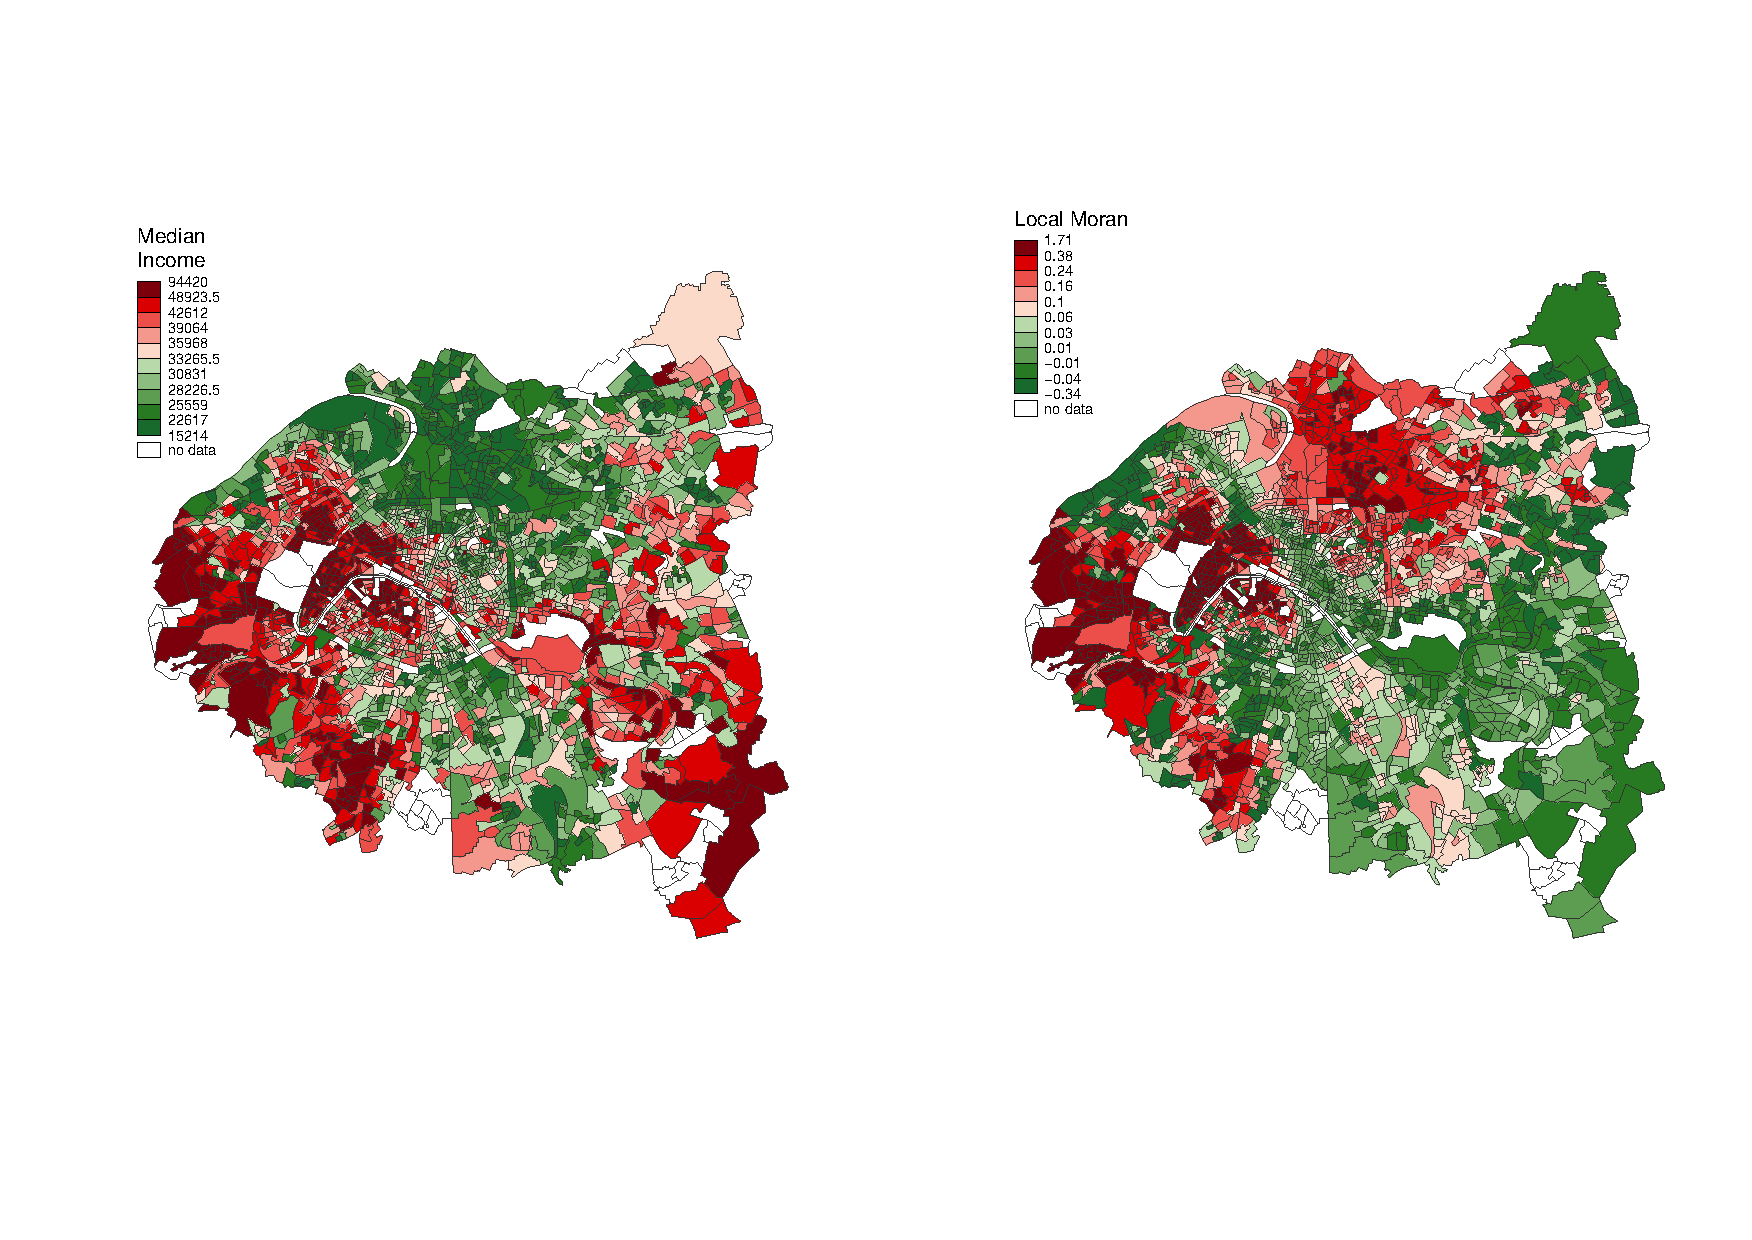
\includegraphics[width=\linewidth]{Figures/RobustnessDiscrepancy/grandParis_income_moran.pdf}
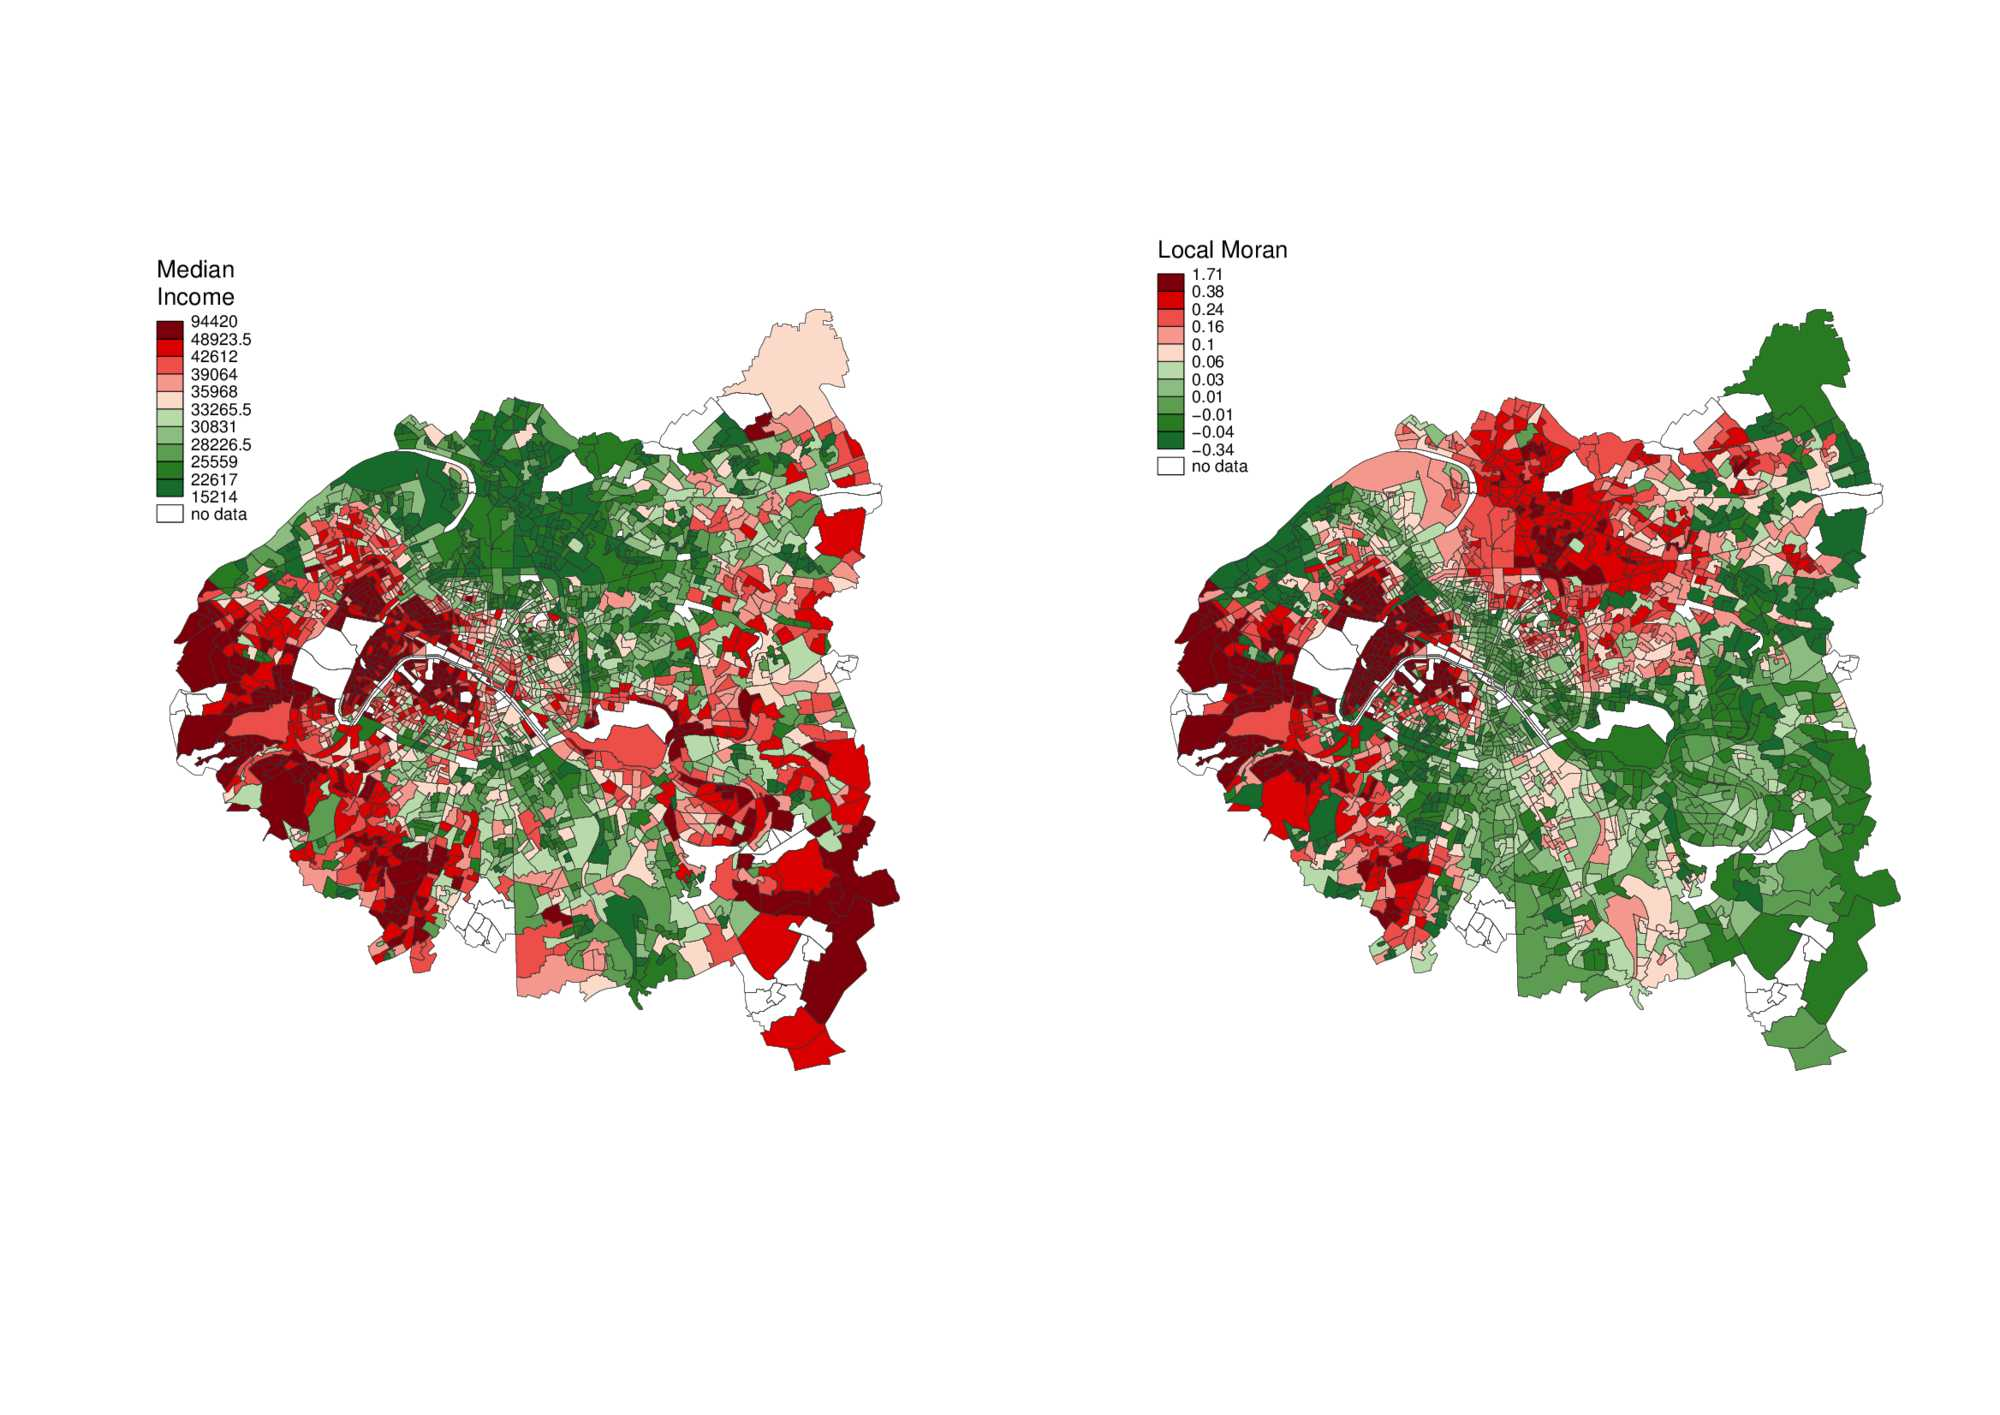
\includegraphics[width=\linewidth]{Figures/Final/B-robustness-segreg.jpg}
\appcaption{\textbf{Maps of Metropolitan Segregation.} Maps show yearly median income on basic statistical units (IRIS) for the three departments constituting mainly the Great Paris metropolitan area, and the corresponding local Moran spatial autocorrelation index, defined for unit $i$ as $\rho_i = N/\sum_{j}w_{ij} \cdot \frac{\sum_{j} w_{ij} (X_j - \bar{X})(X_i - \bar{X})}{\sum_i (X_i - \bar{X})^2}$. The most segregated areas coincide with the richest and the poorest, suggesting an increase of segregation in extreme situations.}{\textbf{Cartes de ségrégation métropolitaine.} Les cartes montrent le revenu annuel médian pour les unités statistiques élémentaires (IRIS) pour les trois départements correspondant globalement à la métropole du Grand Paris, et l'index local d'autocorrelation spatiale de Moran correspondant, défini pour l'unité $i$ par $\rho_i = N/\sum_{j}w_{ij} \cdot \frac{\sum_{j} w_{ij} (X_j - \bar{X})(X_i - \bar{X})}{\sum_i (X_i - \bar{X})^2}$. Les zones les plus ségréguées coincident avec les plus riches et les plus pauvres, suggérant une augmentation de la ségrégation dans les cas extremes.\label{fig:robustness:segreg}}
\end{figure}
%%%%%%%%%%%%%%%%

\paragraph{Results}{Résultats}


\bpar{
We apply our method with these indicators on the Greater Paris area, constituted of four \emph{d{\'e}partements} that are intermediate administrative units. The recent creation of a new metropolitan governance system~\cite{gilli2009paris} underlines interrogations on its consistence, and in particular on its relation to intermediate spatial inequalities. We show in Fig.~\ref{fig:robustness:segreg} maps of spatial distribution of median income and corresponding local index of autocorrelation. We observe the well-known West-East opposition and district disparities inside Paris as they were formulated in various studies, such as~\cite{guerois2009dynamique} through the analysis of real estate transactions dynamics. We then apply our framework to answer a concrete question that has implications for urban policy : \textit{how are the evaluation of segregation within different territories sensitive to missing data ?} To do so, we proceed to Monte Carlo simulations (75 repetitions) during which a fixed proportion of data is randomly removed, and the corresponding robustness index is evaluated with renormalized indicators. Simulations are done on each \emph{department} separately, each time relatively to the robustness of the evaluation of full Greater Paris. Results are shown in Fig. 2. All areas present a slightly better robustness than the reference, what could be explained by local homogeneity and thus more fiable segregation values. Implications for policy that can be drawn are for example direct comparisons between areas : a loss of 30\% of information on 93 area corresponds to a loss of only 25\% in 92 area. The first being a deprived area, the inequality is increased by this relative lower quality of statistical information. The study of standard deviations suggest further investigations as different response regimes to data removal seem to exist.
}{
La méthode est appliquée avec ces indicateurs à la zone du Grand Paris, constitué de 4 département qui sont des niveaux administratifs intermédiaires. La création récente d'un nouveau système de gouvernance métropolitaine~\cite{gilli2009paris} met en évidence des interrogations sur sa pertinence, notamment sur ses capacités d'atténuer les inégalités spatiales. On peut voir en Fig.~\ref{fig:robustness:segreg} les cartes de la distribution spatiale du revenu médian et de l'index local d'autocorrelation spatiale correspondant. La dichotomie bien connue entre est et ouest est retrouvée ainsi que la disparité des quartiers intra-muros, comme cela été présenté par diverses études, comme~\cite{guerois2009dynamique} à travers l'analyse des dynamiques des transactions immobilières. Notre cadre d'étude est ensuite appliqué à une question concrète ayant des implications pour la prise de décision : \textit{dans quelle mesure une évaluation de la ségrégation au sein de différents territoires est sensible aux données manquantes ?} Pour cela, on procède à des simulations de Monte-Carlo (75 répétitions) pour lesquelles une proportion fixe de données est supprimée aléatoirement, et l'indice de robustesse correspondant est évalué avec les indicateurs normalisés. Les simulations sont faites sur chaque département de façon indépendante, à chaque fois pour une robustesse relative à l'évaluation du Grand Paris complet. Les résultats sont présentés en Fig.~\ref{fig:robustness:sensitivity}. Toutes les zones ont une robustesse légèrement meilleure que la référence, ce qui pourrait être expliqué par une homogénéité locale et donc des indices de ségrégation plus fiables. Les implications pour la prise de décision qui peuvent être par exemple tirées sont des comparaisons directes entre les zones : une perte de 30\% de l'information sur le 93 correspond à une perte de seulement 25\% pour le 92. La première zone étant déjà défavorisée socio-économiquement, l'inégalité est augmentée par cette qualité moindre de l'information statistique. L'étude des déviations standard suggère des études plus approfondies comme différents régimes de réponse à la suppression de données semblent exister.
}



%%%%%%%%%%%%%%%%
\begin{figure}
%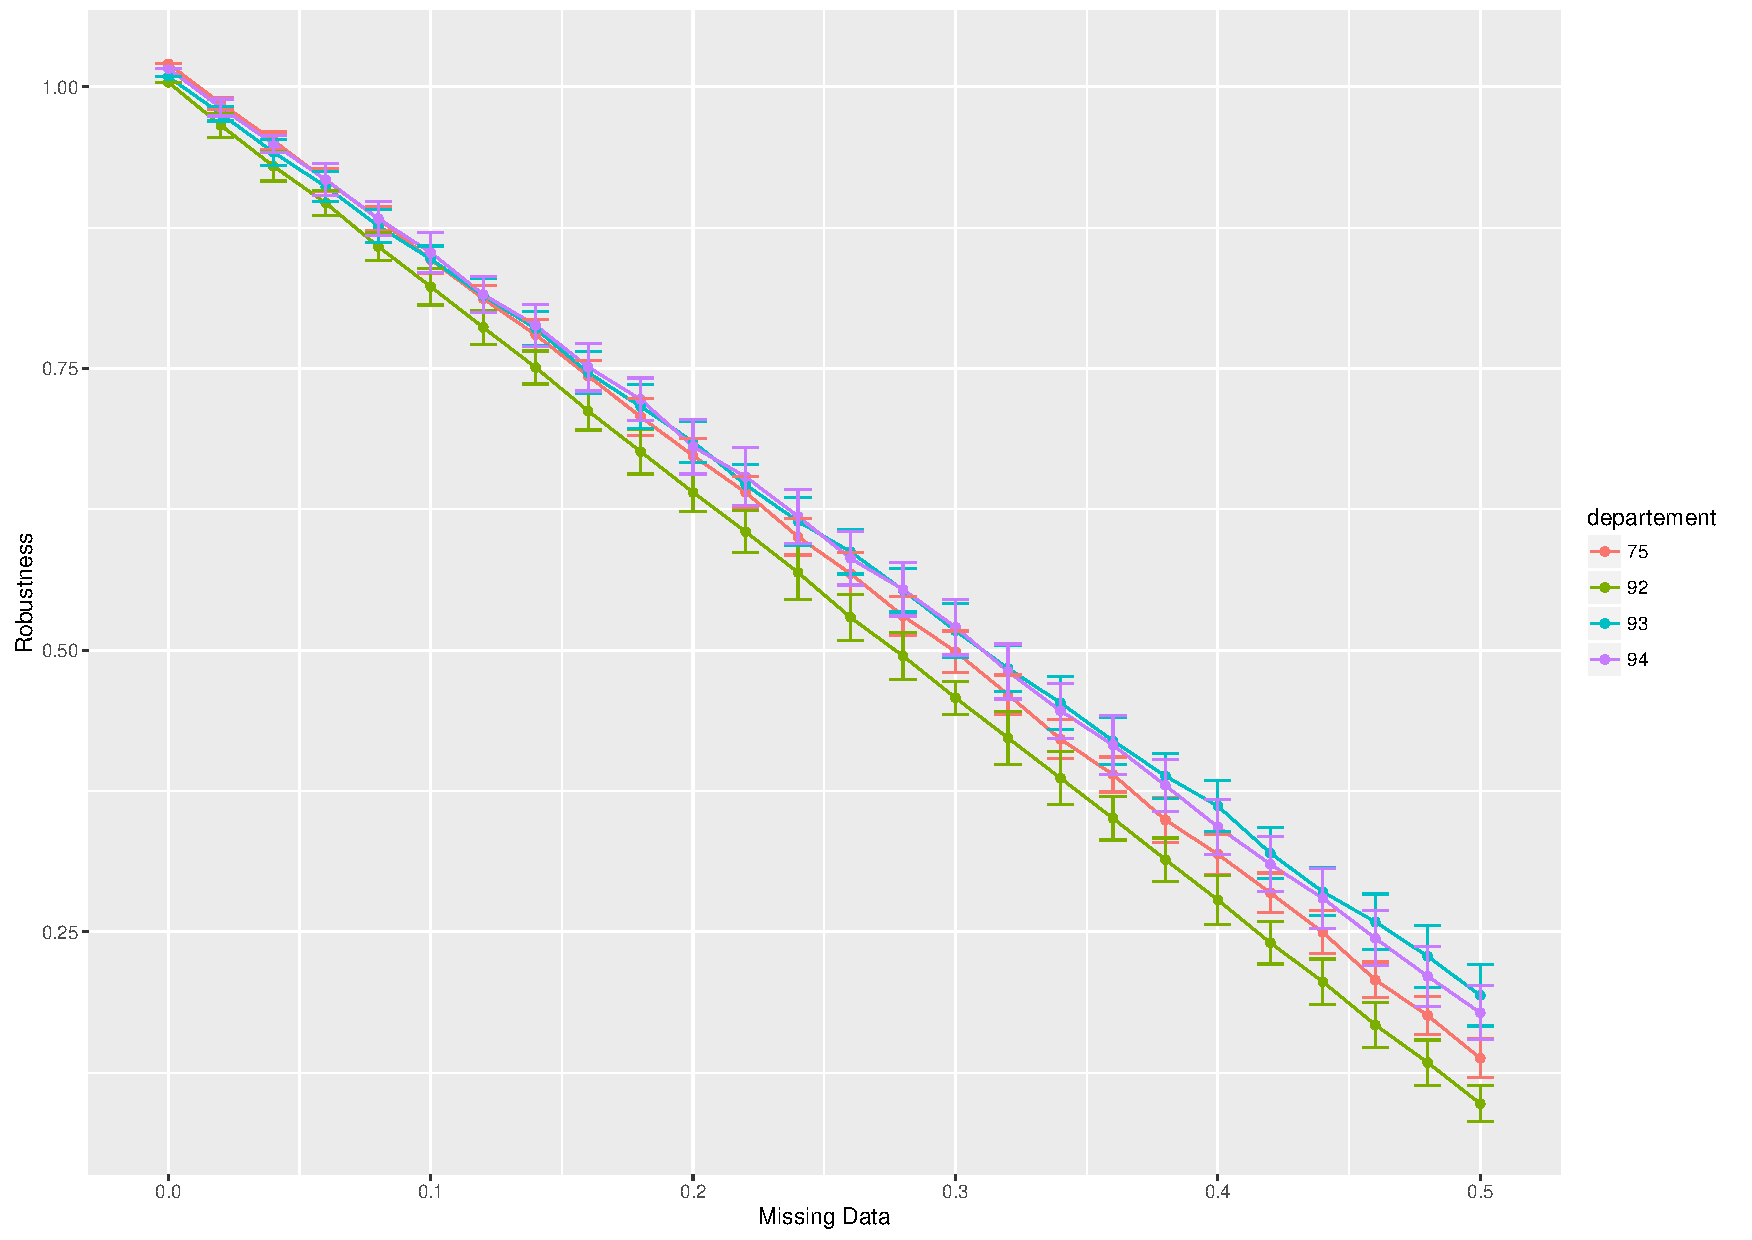
\includegraphics[width=\textwidth]{Figures/RobustnessDiscrepancy/alldeps_rob_renormindics.pdf}
%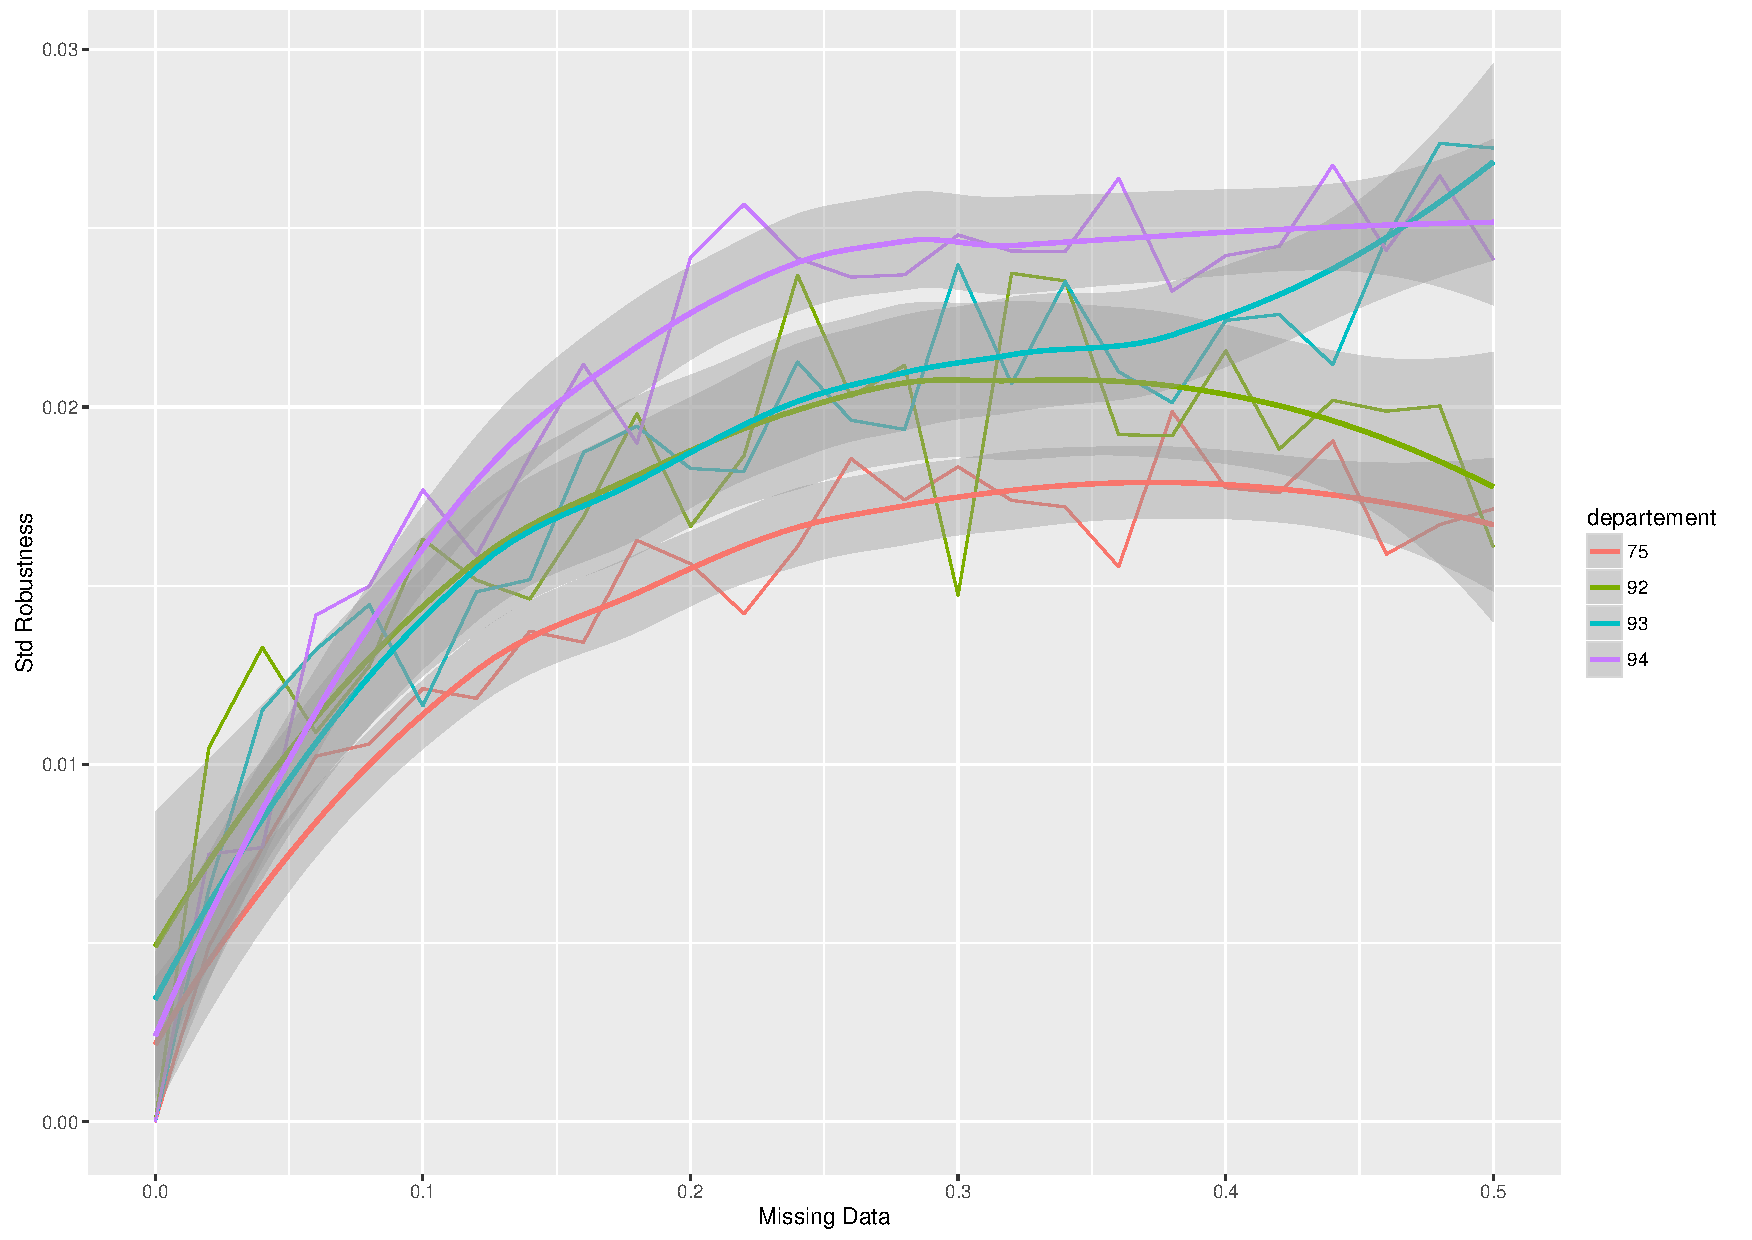
\includegraphics[width=\textwidth]{Figures/RobustnessDiscrepancy/alldeps_robsd_renormindics.pdf}
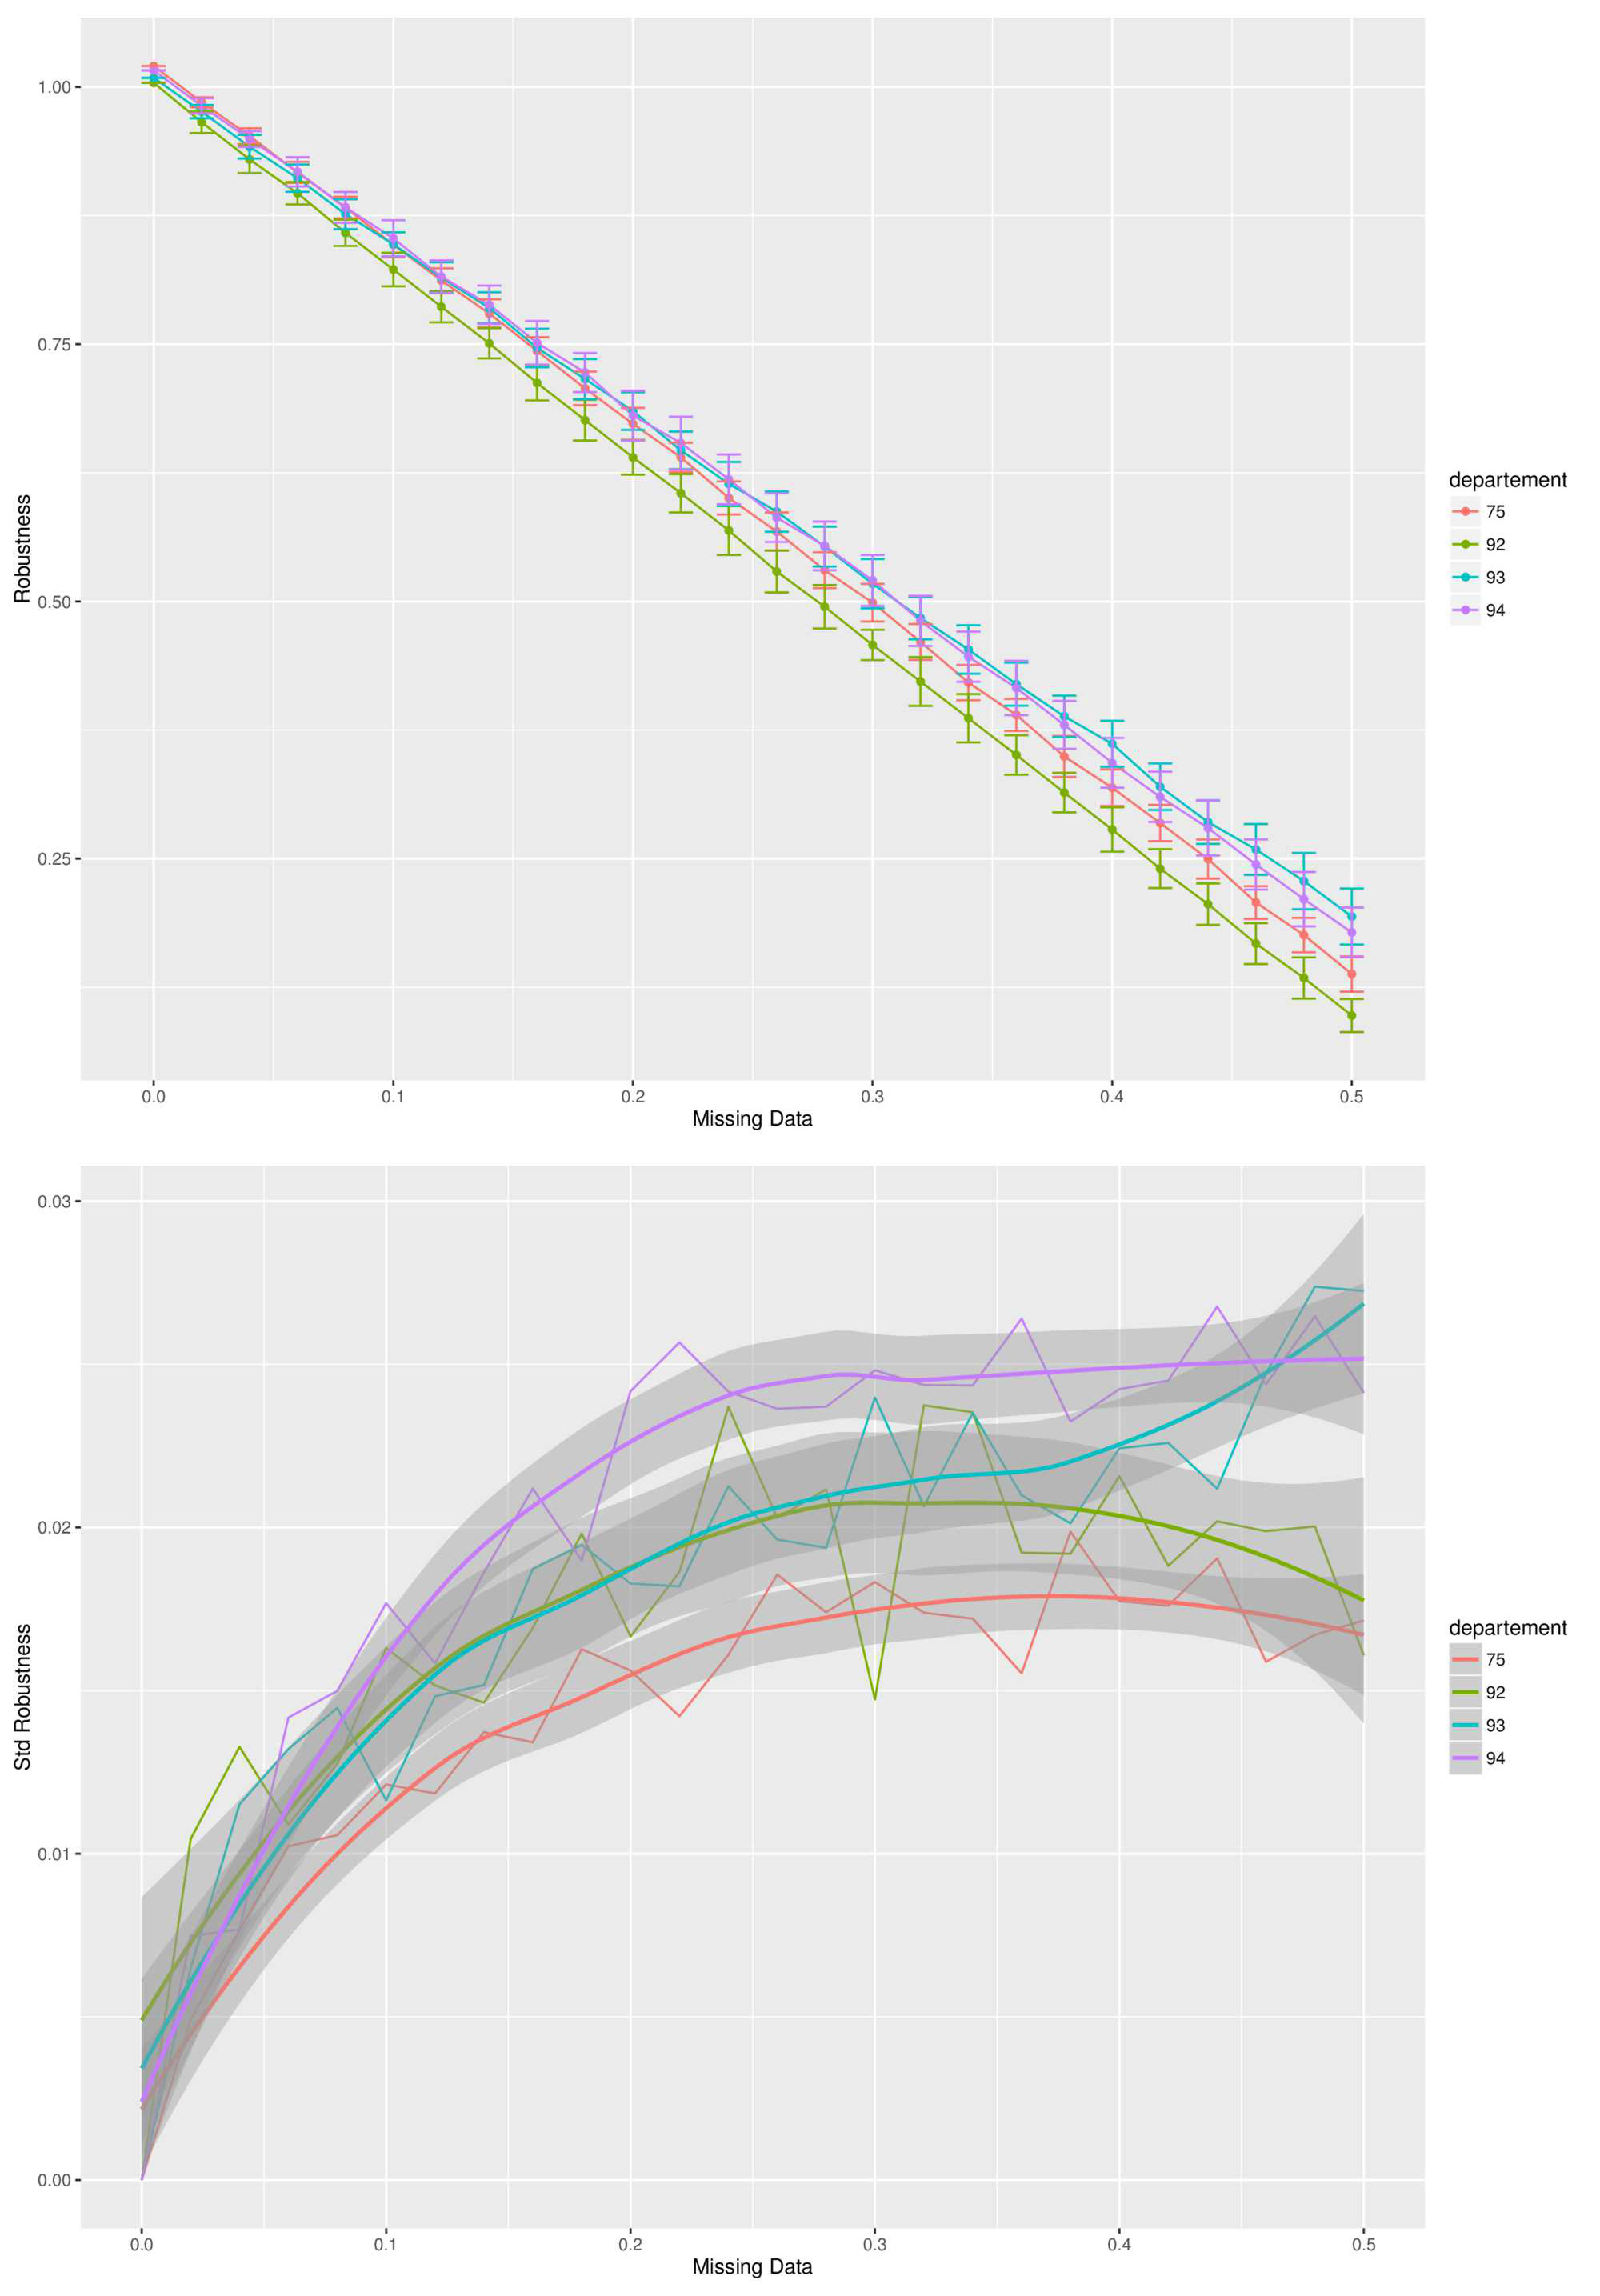
\includegraphics[width=0.9\linewidth]{Figures/Final/B-robustness-sensitivity.jpg}
\appcaption{\textbf{Sensitivity of robustness to missing data.} \textit{Left.} For each department, Monte Carlo simulations (N=75 repetitions) are used to determine the impact of missing data on robustness of segregation evaluation. Robustness ratios are all computed relatively to full metropolitan area with all available data. Quasi-linear behavior translates an approximative linear decrease of discrepancy as a function of data size. The similar trajectory of poorest departments (93,94) suggest the correction to linear behavior being driven be segregation patterns. \textit{Right.} Corresponding standard deviations of robustness ratios. Different regimes (in particular 93 against others) unveil phase transitions at different levels of missing data, meaning that the evaluation in 94 is from this point of view more sensitive to missing data.}{\textbf{Sensibilité de la robustesse aux données manquantes.} \textit{Gauche.} Pour chaque département, des simulations de Monte-Carlo (N=75 répétitions) sont utilisées pour déterminer l'impact des données manquantes sur la robustesse de l'évaluation de la ségrégation. Les ratios de robustesse sont tous calculés relativement à la région métropolitaine complète avec toutes les données disponibles. Le comportement quasi-linéaire traduit une décroissance approximativement linéaire de la discrépance en fonction de la taille des données. Les trajectoires similaires des départements les plus pauvres (93,94) suggère que la correction au comportement linéaire est fonction des motifs de ségrégation. \textit{Droite.} Déviations standard des ratios de robustesse. Les différents régimes (en particulier le 93 contre les autres) révèlent des transitions de phase à différents niveaux de données manquantes, signifiant que l'évaluation dans le 94 est de ce point de vue plus sensible aux données manquantes.\comment{typo département ?}}
\label{fig:robustness:sensitivity}
\end{figure}
%%%%%%%%%%%%%%%%





%%%%%%%%%%%%%%%%
%% Discussion
%%%%%%%%%%%%%%%%
\subsection{Discussion}{Discussion}


%%%%%%%%%%%%%%%%
\subsubsection{Applicability to Real situations}{Applicabilité à des situations réelles}


\paragraph{Implications for Decision-making}{Implications pour la prise de décision}


\bpar{
The application of our method to concrete decision-making can be thought in different ways. First in the case of a comparative multi-attribute decision process, such as the determination of a transportation corridor, the identification of territories on which the evaluation may be flawed (i.e. has a poor relative robustness) could allow a more refined focus on these and a corresponding revision of datasets or an adapted revision of weights. In any case the overall decision-making process should be made more reliable. A second direction lays in the spirit of the real application we have proposed, i.e. the sensitivity of evaluation to various parameters such as missing data. If a decision appears as reliable because data have few missing points, but the evaluation is very sensitive to it, one will be more careful in the interpretation of results and taking the final decision. Further work and testing will however be needed to understand framework behavior in different contexts and be able to pilot its application in various real situations.
}{
L'application de notre méthode à des situations concrètes de prise de décision peu être pensée de différentes manières. Tout d'abord dans le cas d'un processus multi-attributs à but comparatif, comme la détermination d'un corridor pour une nouvelle infrastructure de transport, l'identification des territoires sur lesquels l'évaluation pourrait être biaisée (i.e. avec une mauvaise robustesse relative) devrait permettre une attention particulière pour ceux-ci, et l'adaptation des jeux de données ou la révision des points en conséquence. Dans tous les cas le processus total devrait être plus fiable. Une autre possibilité ressemble à l'application réelle que nous avons développé, i.e. la sensibilité de l'évaluation à divers paramètres comme les données manquantes. Si une décision parait fiable car la taille de données est grande, mais que l'évaluation est très sensible à la suppression de données, il faudra être prudent pour l'interprétation des résultats et pour la prise de décision finale. Un travail approfondi et de test sera cependant nécessaire pour comprendre le comportement du cadre dans différents contextes et pouvoir piloter son application dans des situations réelles diverses.
}


\paragraph{Integration Within Existing Frameworks}{Intégration au sein de cadres existants}


\bpar{
The applicability of the method on real cases will directly depend on its potential integration within existing framework. Beyond technical difficulties that will surely appear when trying to couple or integrate implementations, more theoretical obstacles could occur, such as fuzzy formulations of functions or data types, consistency issues in databases, etc. Such multi-criteria framework are numerous. Further interesting work would be to attempt integration into an open one, such as e.g. the one described in~\cite{tivadar2014oasis} which calculates various indices of urban segregation, as we have already illustrated the application on metropolitan segregation indexes.
}{
L'applicabilité de la méthode à des cas réels dépendra directement de son intégration potentielle dans des environnements existants. Au delà des difficultés techniques qui apparaissent nécessairement en essayant de coupler ou d'intégrer des implémentations existantes, des obstacles plus théoriques pourraient émerger, comme des formulations floues des fonctions ou des types de données, la cohérence des bases de données, etc. De tels cadres multi-critères sont nombreux. Un développement possible serait l'intégration dans un cadre open-source, comme par exemple celui décrit dans~\cite{tivadar2014oasis} qui calcule divers indices de ségrégation urbaine, comme on l'a déjà illustré pour l'application à la ségrégation métropolitaine.
}

\paragraph{Availability of Raw Data}{Disponibilité des données brutes}


\bpar{
In general, sensitive data such as transportation questionnaires, or very fine granularity census data are not openly available but provided already aggregated at a certain level (for instance French Insee Data are publicly available at basic statistical unit level or larger areas depending on variables and minimal population constraints, more precise data is under restricted access). It means that applying the framework may imply complicated data research procedure, its advantage to be flexible being thus reduced through additional constraints.
}{
De manière générale, des données sensibles comme des questionnaires de transport, ou des données de sondage à granularité très fine, ne sont pas disponibles de manière ouverte, mais fournis de manière déjà agrégée à un certain niveau (comme par exemple les données françaises de l'Insee sont disponibles publiquement au niveau des unités statistiques élémentaires ou pour des zones plus grandes selon les variables et des contraintes de population minimale, les données plus précises étant à accès restreint). Cela signifie que l'application de notre cadre peut impliquer une procédure de recherche de données laborieuse, l'avantage d'être flexible étant alors compensé par ces contraintes additionnelles.
}


%%%%%%%%%%%%%%%%
\subsubsection{Validity of Theoretical Assumptions}{Validité des hypothèses théoriques}


\bpar{
A possible limitation of our approach is the validity of the assumption formulating indicators as spatial integrals. Indeed, many socio-economic indicators are not necessarily depending explicitly on space, and trying to associate them with spatial coordinates may become a slippery slope (e.g. associate individual economic variables with individual residential coordinates will have a sense only if the use of the variable has a relation with space, otherwise it is a non-legitimate artifact). Even indicators which have a spatial value may derive from non-spatial variables, as~\cite{kwan1998space} points out concerning accessibility, when opposing integrated accessibility measures with individual-based non necessarily spatial-based (e.g. individual decisions) measures. Constraining a theoretical representation of a system to fit a framework by changing some of its ontological properties (always in the sense of real meaning of objects) can be understood as a violation of a fundamental rule of modeling and simulation in social science given in~\cite{banos2013HDR}, that is that there can be an universal ``language'' for modeling and some can not express some systems, having for consequence misleading conclusion due to ontology breaking in the case of an over-constrained formulation.
}{
Une limitation possible de notre approche est la validité de l'hypothèse qui formule les indicateurs comme des intégrales spatiales. En fait, de nombreux indicateurs socio-économiques ne dépendent pas nécessairement directement de l'espace, et essayer de les associer à des coordonnées peut entraîner sur une pente glissante (par exemple, associer des variables économiques individuelles à des coordonnées résidentielles aura un sens seulement si la variable à une relation à l'espace, autrement un devient un artefact superflu). Même des indicateurs qui ont une valeur spatiale peuvent dériver de variables non-spatiales, comme~ \cite{kwan1998space} le souligne au sujet de l'accessibilité, en opposant les mesures d'accessibilité intégrée aux mesures individu-centrées mais pas forcément basée sur l'espace (comme par exemple des décisions individuelles). Contraindre une représentation théorique d'un système pour le faire rentrer dans un cadre en changeant certaines de ses propriétés ontologiques (toujours dans le sens de la signification réelle des objets) peut être compris comme une violation d'une des règles pour la modélisation et la simulation en sciences sociales données par~\cite{banos2013HDR}, car cela impliquerait qu'il pourrait exister un langage universel pour la modélisation, malgré qu'il ne puisse retranscrire certains systèmes, ayant pour conséquences des conclusions errantes à cause d'une rupture d'ontologie dans le cas d'une formulation sur-contrainte.
}

%%%%%%%%%%%%%%%%
\subsubsection{Framework Generality}{Généralité du Cadre}


\bpar{
We argue that the fundamental advantage of the proposed framework is its generality and flexibility, since robustness of the evaluations are obtained only through data structure if ones relaxes constraints on the value of weight. Further work should go towards a more general formulation, suppressing for example the linear aggregation assumption. Non-linear aggregation functions would require however to present particular properties regarding integral inequalities. For example, similar results could search in the direction of integral inequalities for Lipschitzian functions such as the one-dimensional results of~\cite{dragomir1999ostrowski}.
}{
Nous soutenons qu'un des avantages fondamentaux de notre cadre est sa généralité et sa flexibilité, puisque la robustesse des évaluations est obtenue seulement par la structure des données si l'on relaxe les hypothèses sur les valeurs des poids. Des approfondissement pourraient inclure une formulation plus générale, en supprimant par exemple l'hypothèse d'agrégation linéaire. Des fonctions d'agrégation non-linéaires demanderaient toutefois de vérifier certaines propriétés regardant les inégalités intégrales. Par exemple, des résultats similaires pourraient être obtenus en s'orientant vers des inégalités intégrales pour fonctions Lipschitziennes, comme les résultats en une dimension de~\cite{dragomir1999ostrowski}.
}


%%%%%%%%%%%%%%%%
%% Conclusion
%%%%%%%%%%%%%%%%
\subsection*{Conclusion}{Conclusion}


\bpar{
We have proposed a model-independent framework to compare the robustness of multi-attribute evaluations between different urban systems. Based on data discrepancy, it provide a general definition of relative robustness without any assumption on model for the system, but with limiting assumptions that are the need of linear aggregation and of indicators being expressed through spatial kernel integrals. We propose a toy implementation based on real data for the city of Paris, numerical results confirming general expected behavior, and an implementation on real data for income segregation on Greater Paris metropolitan areas, giving possible insights into concrete policy questions. Further work should be oriented towards sensitivity analysis of the method, application to other real cases and theoretical assumptions relaxation, i.e. the relaxation of linear aggregation and spatial integration.
}{
Nous avons proposé un cadre indépendant du modèle pour comparer la robustesse d'évaluations multi-attributs entre différents systèmes urbains. A partir de la discrépance des données, on fournit une définition générale de la robustesse relative sans aucune hypothèse de modèle pour le système, mais en supposant une agrégation linéaire des objectifs et des indicateurs exprimés comme des intégrales à noyaux. Nous proposons une première implémentation preuve de concept pour la ville de Paris pour laquelle les résultats numériques confirment la tendance générale attendue, et une implémentation sur des données réelles pour la ségrégation de revenus pour la région métropolitaine du Grand Paris, fournissant des réponses possibles à des questions de prise de décision plus concrètes. Des développements possibles peuvent inclure une analyse de sensibilité de la méthode, des applications à d'autres cas réels et une relaxation des hypothèses théoriques, c'est à dire de l'agrégation linéaire et de l'intégration spatiale.\comment{confusion spatial/ kernel ? -> idem à l'oral ?}
}


%\section*{Acknowledgments}

%The author would like to thank Julien Keutchayan (Ecole Polytechnique de Montr{\'e}al) for suggesting the original idea of using discrepancy, and anonymous reviewers for the useful comments and insights.




%%%%%%%%%%%%%%%%%%%%%%%%%%%%%


%%%%%%%%%%%%%%%%%%
%% Appendix : Morphogenesis



% Chapter 

%\chapter{Urban Morphogenesis}{Morphogenèse Urbaine} % Chapter title
\chapter{Morphogenèse Urbaine}

\label{ch:morphogenesis} % For referencing the chapter elsewhere, use \autoref{ch:name} 

%----------------------------------------------------------------------------------------

%\headercit{}{}{}

%\bigskip


Il est bien établi en géographie l'importance des relations spatiales et de la mise en réseau, comme le formule \noun{Tobler} par sa ``première loi de la géographie''~\cite{tobler2004first}\comment[FL]{la citer}.\comment[CC]{phrase a reformuler: les relations spatiales ... sont bien etablies en geo, et comme le prouve par ex. la premiere loi de la geo de tobler "..."} Nous l'avons mis en évidence pour les relations entre réseaux et territoires par exemple en section~\ref{sec:interactiongibrat}. Toutefois, les travaux sur la non-stationnarité et la non-ergodicité, ainsi que la mise en valeur d'échelles locales endogènes, suggèrent une certaine pertinence à l'idée de sous-système relativement indépendant, au sens où il serait possible d'isoler certaines règles locales régissant celui-ci étant fixés certains paramètres exogène\comment[CC]{s} capturant justement les relations avec d'autres sous-systèmes\comment[CC]{pas clair. plutot faire 3 phrases sinon on perd completement le sens}. Cette question porte à la fois sur l'échelle d'espace, de temps, mais aussi sur les éléments concernés. Reprenons un exemple concret de terrain déjà évoqué en Chapitre~\ref{ch:thematic}: la laborieuse mise en place du tramway de Zhuhai. L'impact du retard de la mise en place et la remise en question de futures lignes, dus à un problème technique inattendu lié à une technologie de transfert de courant par troisième rail importée d'Europe qui n'avait jamais été testée dans les conditions climatiques locales, assez exceptionnelles en termes d'humidité, aura une nature très différentes selon l'échelle et les agents considérés\comment[CC]{hierarchise cette phrase: les details entre parentheses et l'info principale mise en valeur "le retard et l'incertitude affecte differents acteurs differement}. Le manque de coordination générale entre transports et urbanisme laisse supposer que les dynamiques urbaines en terme\comment[CC]{s} de populations et d'emplois y sont relativement insensibles à court terme\comment[FL]{sens ?}. Le Bureau des Transports de la Municipalité ainsi que le bureau technique Européen ont pu subir des répercussions politiques et économiques bien plus graves\comment[FL]{$\sim$}\comment[CC]{quel rapport? on est toujours a Zhuhai ou pas?}. D'autre part, que ce soit à Zhongshan, Macao ou Hong-Kong le problème a une repercussion quasi-nulle\comment[CC]{c'est un resultat ou une supposition? Avant de generaliser, a ta place, j'interpreterais cette info d'abord: dans ces 3 villes, pas d'incidence car connexion faible et diffferents sous-systemes qui amortissent}. Généralisant au système de transport local, celui-ci peut être relativement bien isolé des systèmes voisins ou à plus grande échelle\comment[CC]{supprimer "ou a plus grande echelle}, et donc ses relations avec la ville considérée dans un contexte local. On supposera à la fois une certaine forme de stationnarité locale (``régime urbain local'') mais aussi une certaine indépendance avec l'extérieur. Dans ce cadre, son auto-organisation locale impliquera nécessairement des relations fortes entre forme et fonction, de par la distribution spatiale des fonctions urbaines mais aussi car \emph{la forme fait la fonction} dans certains cas de figure, au sens des motifs d'utilisation entièrement conditionnés à cette forme\comment[CC]{je vois pas le lien avec les phrases precedentes}. Le type de raisonnement que nous avons esquissé mobilise les éléments essentiels propres à l'idée de \emph{morphogenèse urbaine}. Nous allons dans ce chapitre clarifier sa définition et montrer les potentialité\comment[CC]{s} qu'elle donne pour éclairer les relations entre réseaux et territoires. La morphogenèse, qui a été importée de la biologie vers de nombreux champs, a dans chaque cas ouvert des voies pour l'étude des systèmes complexes propres à ce champ selon un point particulier. Il est important de noter que le monument qu'est la Théorie des Catastrophes de \noun{René Thom} introduit une façon originale de comprendre la différentiation qualitative et donc la morphogenèse. Cette théorie, très mal comprise \comment[CC]{par qui? est-ce que c'est important dans ton argumentation ici? sinon ca fait un peu pedanterie gratuite}, contient un potentiel d'application immense aux problèmes qui nous concernent, comme l'a effleuré \comment[CC]{id} \noun{Durand-Dastès}~\cite{durand2003geographes} en évoquant la systèmogenèse, que nous développerons en ouverture. Dans un premier temps, un effort d'épistémologie par des points de vue complémentaires de plusieurs disciplines permet d'éclairer la nature de la morphogenèse dans la section~\ref{sec:interdiscmorphogenesis}. Cela permet de clarifier le concept en lui donnant une définition bien précise, distincte de celle de l'auto-organisation, qui appuie les relations causales circulaires entre forme et fonction. Nous explorons ensuite un modèle simple de morphogenèse urbaine, basé sur la densité de population seule, à l'échelle mesoscopique, dans la section~\ref{sec:densitygeneration}. La démonstration que les processus abstraits d'agrégation et de diffusion sont suffisants pour reproduire l'ensemble des formes d'établissements humains en Europe, en utilisant les résultats de~\ref{sec:staticcorrelations}, confirme la pertinence de l'idée de morphogenèse pour la modélisation à certaines échelles et pour certains aspects\comment[CC]{lesquels? si tu ne les mentionnes pas, ca n'apporte aucune information}. Ce modèle est ensuite couplé de manière séquentielle à un module de morphogenèse de réseau dans la section~\ref{sec:correlatedsyntheticdata}, afin d'établir un espace faisable \comment[CC]{faisable? ou bien plutot theorique / potentiel / possible} des correlations statiques entre indicateurs de forme urbaine et indicateurs de réseau, qui sont comme on l'a vu précédemment un témoin des relations locales entre réseaux et territoires \comment[CC]{cool}. Celui-ci s'avère relativement large, ce qui confirmera l'utilisation de ce type de modèle de manière fortement couplée par la suite\comment[CC]{pourquoi? il faut expliquer tes conclusions car ca n'est pas evident}.




\stars


\textit{Ce chapitre est composé de divers travaux. La première section est adaptée d'un travail en anglais en collaboration avec \noun{C. Antelope}, \noun{L. Hubatsch} et \noun{J.M. Serna} à la suite de l'école d'été 2016 du Santa Fe Institute~\cite{antelope2016interdisciplinary}; la deuxième section est traduite de~\cite{} \comment[CC]{pas de ref.}; et enfin la troisième section a été écrite pour les Actes des Journées de Rochebrune 2016~\cite{raimbault2016generation}.}



\comment[CC]{Attention. Les parties traduites sont tres claires et avec un niveau de langage soigne, tandis que les introductions / transitions sont brouillonnes et touffues. Il faudrait harmoniser le tout, c'est a dire surtout fluidifier les transitions qui sont la partie en propre de ton manuscript de these, le reste etant deja publie ailleur}





%----------------------------------------------------------------------------------------










%%%%%%%%%%%%%%%%%%


%%%%%%%%%%%%%%%%%%
%% Appendix : Synthetic Data (introduction and financial development)

\newpage

\section{Generation of Correlated Synthetic Data}{Données synthétiques corrélées : Séries temporelles financières} % Chapter title

\label{app:sec:syntheticdata-finance} % For referencing the chapter elsewhere, use \autoref{ch:name} 

%----------------------------------------------------------------------------------------


%%%%%%%%%%%%%%%%%%%%%%
\subsection*{Context}{Contexte}

\bpar{
Our first field of application is that of financial complex systems, of which captured signals, financial time-series, are heterogeneous, multi-scalar and highly non-stationary~\cite{mantegna1999introduction}. Correlations have already been the object of a broad bunch of related literature. For example, Random Matrix Theory allows to undress signal of noise, or at least to estimate the proportion of information undistinguishable from noise, for a correlation matrix computed for a large number of asset with low-frequency signals (daily returns mostly)~\cite{2009arXiv0910.1205B}. Similarly, Complex Network Analysis on networks constructed from correlations, by methods such as Minimal Spanning Tree~\cite{2001PhyA..299...16B} or more refined extensions developed for this purpose~\cite{tumminello2005tool}, yielded promising results such as the reconstruction of economic sectors structure. At high frequency, the precise estimation of of interdependence parameters in the framed of fixed assumptions on asset dynamics, has been extensively studied from a theoretical point of view aimed at refinement of models and estimators~\cite{barndorff2011multivariate}. Theoretical results must be tested on synthetic datasets as they ensure a control of most parameters in order to check that a predicted effect is indeed observable \emph{all things equal otherwise}. For example, \cite{potiron2015estimation} obtains a bias correction for the \emph{Hayashi-Yoshida} estimator (used to estimate integrated covariation between two brownian at high frequency in the case of asynchronous observation times) by deriving a central limit theorem for a general model that endogeneize observation times. Empirical confirmation of estimator improvement is obtained on a synthetic dataset at a fixed correlation level.
}{
Un domaine d'application proposé pour la méthode de données synthétiques présentée en~\ref{app:sec:syntheticdata} est celui des séries temporelles financières, signaux typiques de systèmes complexes hétérogènes et multiscalaires~\cite{mantegna1999introduction} et pour lesquels les corrélations ont fait l'objet d'abondants travaux. Ainsi, l'application de la théorie des matrices aléatoires peut permettre de débruiter, ou du moins d'estimer la part de signal noyée dans le bruit, une matrice de correlations pour un grand nombre d'actifs échantillonnés à faible fréquence (retours journaliers par exemple)~\cite{2009arXiv0910.1205B}. De même, l'analyse de réseaux complexes construits à partir des corrélations, selon des méthodes type arbre couvrant minimal~\cite{2001PhyA..299...16B} ou des extensions raffinées pour cette application précise~\cite{tumminello2005tool}, ont permis d'obtenir des résultats prometteurs, tels la reconstruction de la structure économique des secteurs d'activités. A haute fréquence, l'estimation précise de paramètres d'interdépendance dans le cadre d'hypothèses fixées sur la dynamique, fait l'objet d'importants travaux théoriques dans un but de raffinement des modèles et des estimateurs~\cite{barndorff2011multivariate}. Les résultats théoriques doivent alors être testés sur des jeux de données synthétiques, qui permettent de contrôler un certain nombre de paramètres et de s'assurer qu'un effet prédit par la théorie est bien observable \emph{toutes choses égales par ailleurs}. Par exemple, \cite{potiron2015estimation} dérive une correction du biais de l'estimateur de \emph{Hayashi-Yoshida} qui est un estimateur de la covariance de deux browniens corrélés à haute fréquence dans le cas de temps d'observation asynchrones, par démonstration d'un théorème de la limite centrale pour un modèle généralisé endogénéisant les temps d'observations. La confirmation empirique de l'amélioration de l'estimateur est alors obtenue sur un jeu de données synthétiques à un niveau de corrélation fixé.
}


%%%%%%%%%%%%%%%%%%%%%%
\subsection*{Formalization}{Formalisation}

\subsubsection*{Framework}{Cadre}


\bpar{
We consider a network of assets $(X_i(t))_{1\leq i \leq N}$ sampled at high-frequency (typically 1s). We use a multi-scalar framework (used e.g. in wavelet analysis approaches~\cite{ramsey2002wavelets} or in multi-fractal signal processing~\cite{bouchaud2000apparent}) to interpret observed signals as the superposition of components at different time scales : $X_i=\sum_{\omega}{X_i^{\omega}}$. We denote by $T_i^{\omega} = \sum_{\omega' \leq \omega} X_i^{\omega}$ the filtered signal at a given frequency $\omega$. A recurrent problem in the study of complex systems is the prediction of a trend at a given scale. It can be viewed as the identification of regularities and their distinction from components considered as random\footnote{see~\cite{gell1995quark} for an extended discussion on the construction of \emph{schema} to study complex adaptive systems (by complex adaptive systems).}. For the sake of simplicity, we represent such a process as a trend prediction model at a given temporal scale $\omega_1$, formally an estimator $M_{\omega_1} : (T_i^{\omega_1}(t'))_{t'<t} \mapsto \hat{T_i}^{\omega_1}(t)$ which aims to minimize error on the real trend $\norm{T_i^{\omega_1} - \hat{T}_i^{\omega_1}}$. In the case of autoregressive multivariate estimators, the performance will depend among other parameters on respective correlations between assets. It is thus interesting to apply the method to the evaluation of performance as a function of correlation at different scales. We assume a Black-Scholes dynamic for assets~\cite{jarrow1999honor}, i.e. $dX = \sigma\cdot dW$, with $W$ Wiener process. Such a dynamic model allows an easy modulation of correlation levels.
}{
Considérons un réseau d'actifs $(X_i(t))_{1\leq i \leq N}$ échantillonnés à haute fréquence (typiquement 1s). On se place dans un cadre multi-scalaire (utilisé par exemple dans les approches par ondelettes~\cite{ramsey2002wavelets} ou analyses multifractales du signal~\cite{bouchaud2000apparent}) pour interpréter les signaux observés comme la superposition de composantes à des multiples échelles temporelles : $X_i=\sum_{\omega}{X_i^{\omega}}$. On notera $T_i^{\omega} = \sum_{\omega' \leq \omega} X_i^{\omega}$ le signal filtré à une fréquence $\omega$ donnée. Prédire l'évolution d'une composante à une échelle donnée est alors un problème caractéristique de l'étude des systèmes complexes, pour lequel l'enjeu est l'identification de régularités et leur distinction des composantes considérées comme stochastiques en comparaison\footnote{voir~\cite{gell1995quark} pour une discussion étendue sur la construction de \emph{schema} pour l'étude de systèmes complexes adaptatifs (par des systèmes complexes adaptatifs).}. Dans un souci de simplicité, on représente un tel processus par un modèle de prédiction de tendance à une échelle temporelle $\omega_1$ donnée, formellement un estimateur $M_{\omega_1} : (T_i^{\omega_1}(t'))_{t'<t} \mapsto \hat{T_i}^{\omega_1}(t)$ dont l'objectif est la minimisation de l'erreur sur la tendance réelle $\norm{T_i^{\omega_1} - \hat{T}_i^{\omega_1}}$. Dans le cas d'estimateurs auto-regressifs multivariés, la performance dépendra entre autre des correlations respectives entre actifs et il est alors intéressant d'utiliser la méthode pour évaluer celle-ci en fonction de niveaux de correlation à plusieurs échelles. On assume une dynamique de Black-Scholes~\cite{jarrow1999honor} pour les actifs, i.e. $dX = \sigma\cdot dW$ avec $W$ processus de Wiener, ce qui permettra d'obtenir facilement des niveaux de correlation voulus.
}


\subsubsection*{Data generation}{Génération des données}


\bpar{
We can straightforward generate $\tilde{X}_i$ such that $\Varb{\tilde{X}_i^{\omega_1}}=\Sigma R \Sigma$ (with $\Sigma$ estimated standard deviations and $R$ fixed correlation matrix) and verifying $X_i^{\omega \leq \omega_0} = \tilde{X}_i^{\omega \leq \omega_0}$ (data proximity indicator : components at a lower frequency than a fundamental frequency $\omega_0 < \omega_1$ are identical). We use therefore the simulation of Wiener processes with fixed correlation. Indeed, if $dW_1 \indep dW_1^{\indep}$ (and $\sigma_1 < \sigma_2$ indicatively, assets being interchangeable), then
\[
W_2 = \rho_{12}W_1 + \sqrt{1-\frac{\sigma_1^2}{\sigma_2^2}\cdot\rho_{12}^2}\cdot W_1^{\indep}
\]
is such that $\rho(dW_1,dW_2)=\rho_{12}$. Next signals are constructed the same way by Gram orthonormalization. We isolate the component at the desired frequency $\omega_1$ by filtering the signal, i.e. $\tilde{X}_i^{\omega_1} = W_i - \mathcal{F}_{\omega_0}[W_i]$ (with $\mathcal{F}_{\omega_0}$ low-pass filter with cut-off frequency $\omega_0$). We reconstruct then the hybrid synthetic signals by 
\begin{equation}
\tilde{X}_i = T_i^{\omega_0} + \tilde{X}_i^{\omega_1}
\end{equation}
}{
Il est alors aisé de générer $\tilde{X}_i$ tel que $\Varb{\tilde{X}_i^{\omega_1}}=\Sigma R$ ($\Sigma$ variance estimée et $R$ matrice de corrélation fixée), par la simulation de processus de Wiener au niveau de corrélation fixé et tel que $X_i^{\omega \leq \omega_0} = \tilde{X}_i^{\omega \leq \omega_0}$ (critère de proximité au données : les composantes à plus basse fréquence qu'une fréquence fondamentale $\omega_0 < \omega_1$ sont identiques). En effet, si $dW_1 \indep dW_1^{\indep}$ (et $\sigma_1 < \sigma_2$ pour fixer les idées, quitte à échanger les actifs), alors $W_2 = \rho_{12}W_1 + \sqrt{1-\frac{\sigma_1^2}{\sigma_2^2}\cdot\rho_{12}^2}W_1^{\indep}$ est tel que $\rho(dW_1,dW_2)=\rho_{12}$. Les signaux suivants sont construits de la même manière par orthonormalisation de Gram. On isole alors la composante à la fréquence $\omega_1$ voulue par filtrage, c'est à dire $\tilde{X}_i^{\omega_1} = W_i - \mathcal{F}_{\omega_0}[W_i]$ (avec $\mathcal{F}_{\omega_0}$ filtre passe-bas à fréquence de coupage $\omega_0$), puis on reconstruit les signaux synthétiques par $\tilde{X}_i = T_i^{\omega_0} + \tilde{X}_i^{\omega_1}$.
}




\subsection*{Results}{Résultats}

\subsubsection*{Methodology}{Méthodologie}



\bpar{
The method is tested on an example with two assets from foreign exchange market (EUR/USD and EUR/GBP), in a six month period from June 2015 to November 2015. Data\footnote{obtained from \texttt{http://www.histdata.com/}, without specified licence. For the respect of copyright, only cleaned and filtered at $\omega_m$ data are made openly available.} cleaning, starting from original series sampled at a frequency around 1s, consists in a first step to the determination of the minimal common temporal range (missing sequences being ignored, by vertical translation of series, i.e. $S(t):=S(t)\cdot \frac{S(t_{n})}{S(t_{n-1})}$ when $t_{n-1},t_n$ are extremities of the ``hole'' and $S(t)$ value of the asset, what is equivalent to keep the constraint to have returns at similar temporal steps between assets). We study then \emph{log-prices} and \emph{log-returns}, defined by $X(t):=\log{\frac{S(t)}{S_0}}$ and $\Delta X (t) = X(t) - X(t-1)$. Raw data are filtered at a maximal frequency $\omega_m = 10\textrm{min}$ (which will be the maximal frequency for following treatments) for concerns of computational efficiency\footnote{as time-series are then sampled at $3\cdot\omega_m$ to avoid aliasing, a day of size 86400 for 1s sampling is reduced to a much smaller size of 432.}. We use a non-causal gaussian filter of total width $\omega$. We fix the fundamental frequency $\omega_0=24\textrm{h}$ and we propose to construct synthetic data at frequencies $\omega_1 = 30\textrm{min},1\textrm{h},2\textrm{h}$. See Fig.~\ref{fig:syntheticdata:example_signal} for an example of signal structure at these different scales.
}{
La méthode est testée sur un exemple de deux actifs du marché des devises (EUR/USD et EUR/GBP), sur une période de 6 mois de juin 2015 à novembre 2015. Le nettoyage des données\footnote{obtenues depuis \texttt{http://www.histdata.com/}, sans licence spécifiée, les données nettoyées et filtrées à $\omega_m$ uniquement sont mises en accessibilité pour respect du copyright.}, originellement échantillonnées à l'ordre de la seconde, consiste dans un premier temps à la détermination du support temporel commun maximal (les séquences manquantes étant alors ignorées, par translation verticale des séries, i.e. $S(t):=S(t)\cdot \frac{S(t_{n})}{S(t_{n-1})}$ lorsque $t_{n-1},t_n$ sont les extrémités du ``trou'' et $S(t)$ la valeur de l'actif, ce qui revient à garder la contrainte d'avoir des retours à pas de temps similaires entre actifs). On étudie alors les \emph{log-price} et \emph{log-returns}, définis par $X(t):=\log{\frac{S(t)}{S_0}}$ et $\Delta X (t) = X(t) - X(t-1)$. Les données brutes sont filtrées à une fréquence $\omega_m = 10\textrm{min}$ (qui sera la fréquence maximale d'étude) pour un souci de performance computationnelle. On utilise un filtre gaussien non causal de largeur totale $\omega$. On fixe $\omega_0=24\textrm{h}$ et on se propose de construire des données synthétiques aux fréquences $\omega_1 = 30\textrm{min},1\textrm{h},2\textrm{h}$. Voir la figure~\ref{fig:syntheticdata:example_signal} pour un exemple de la structure du signal à ce différentes échelles.
}


%%%%%%%%%%%%%%%%%%%
\begin{figure}%[h!]
%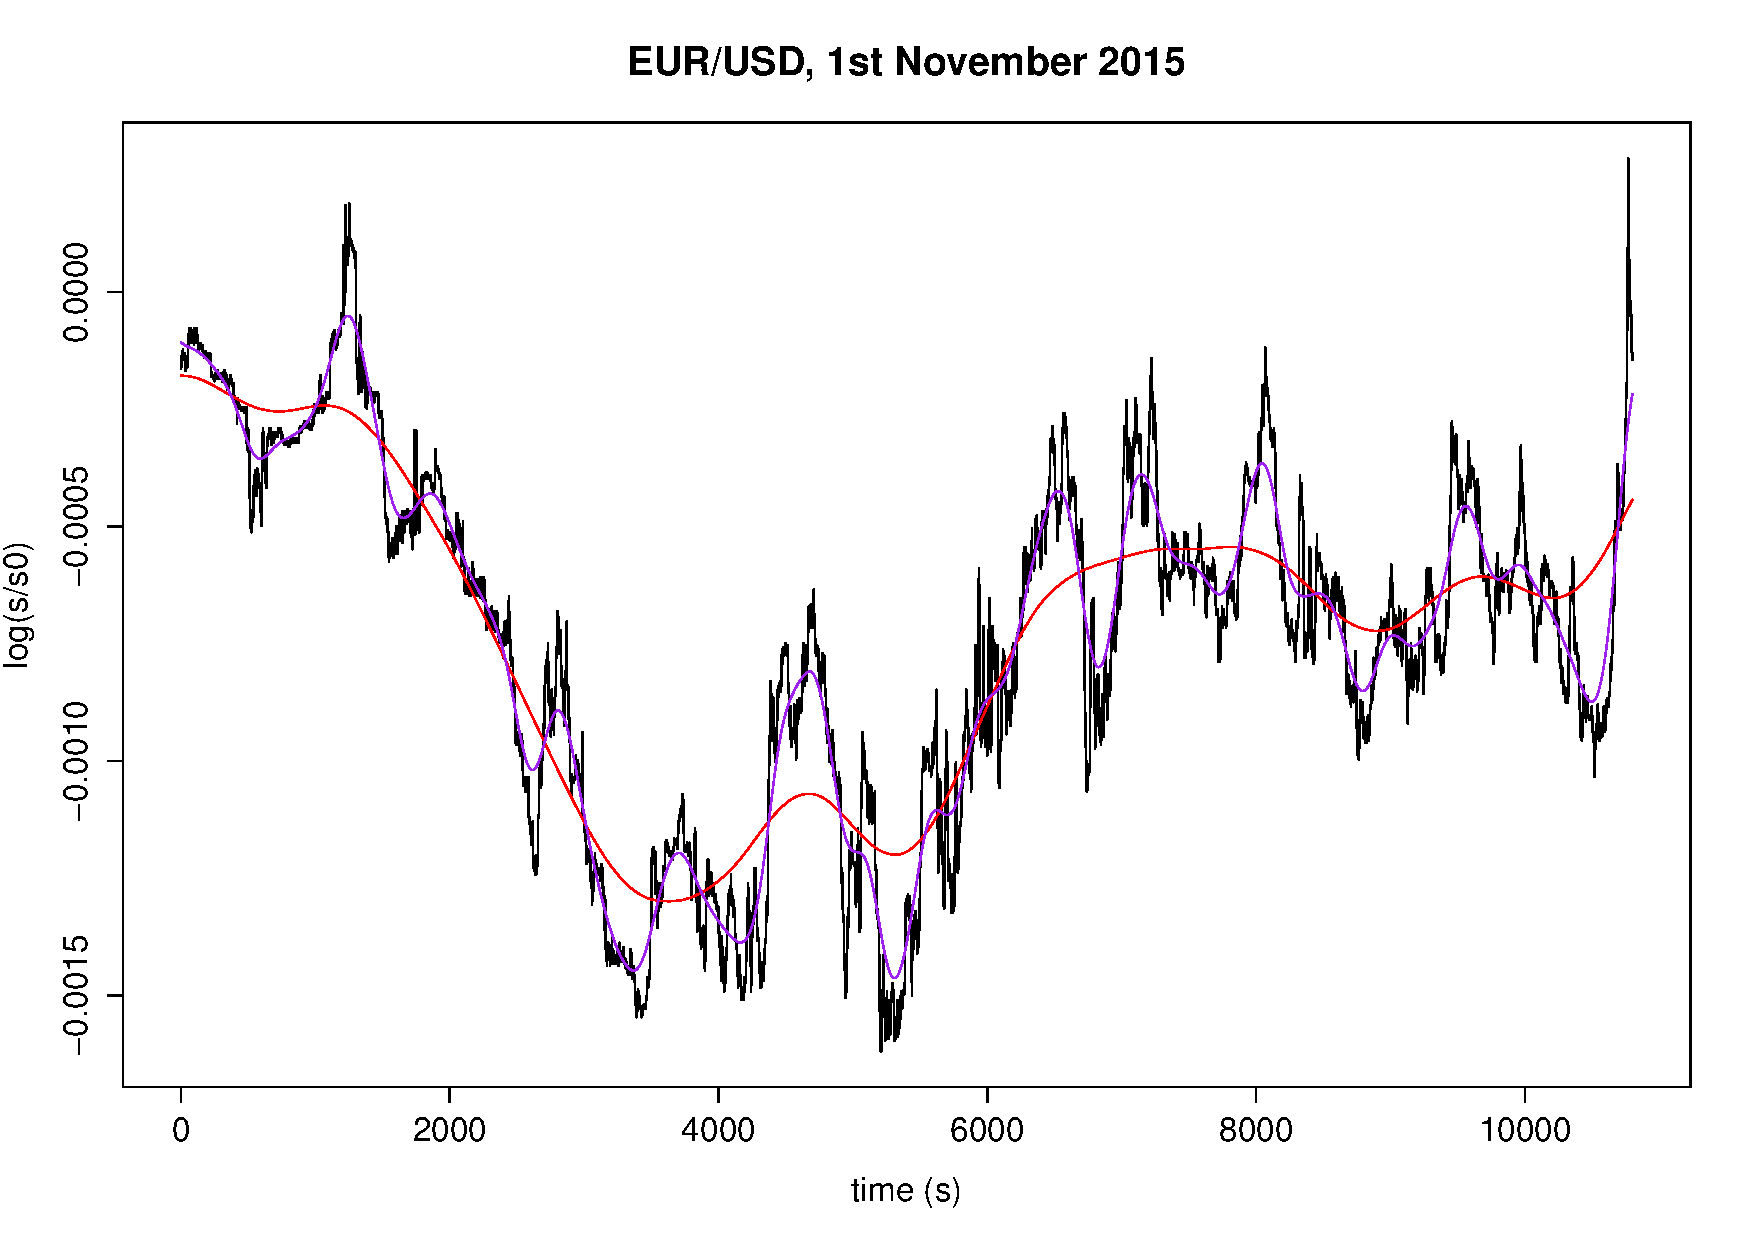
\includegraphics[width=\textwidth]{Figures/SyntheticData/ex_filtering}
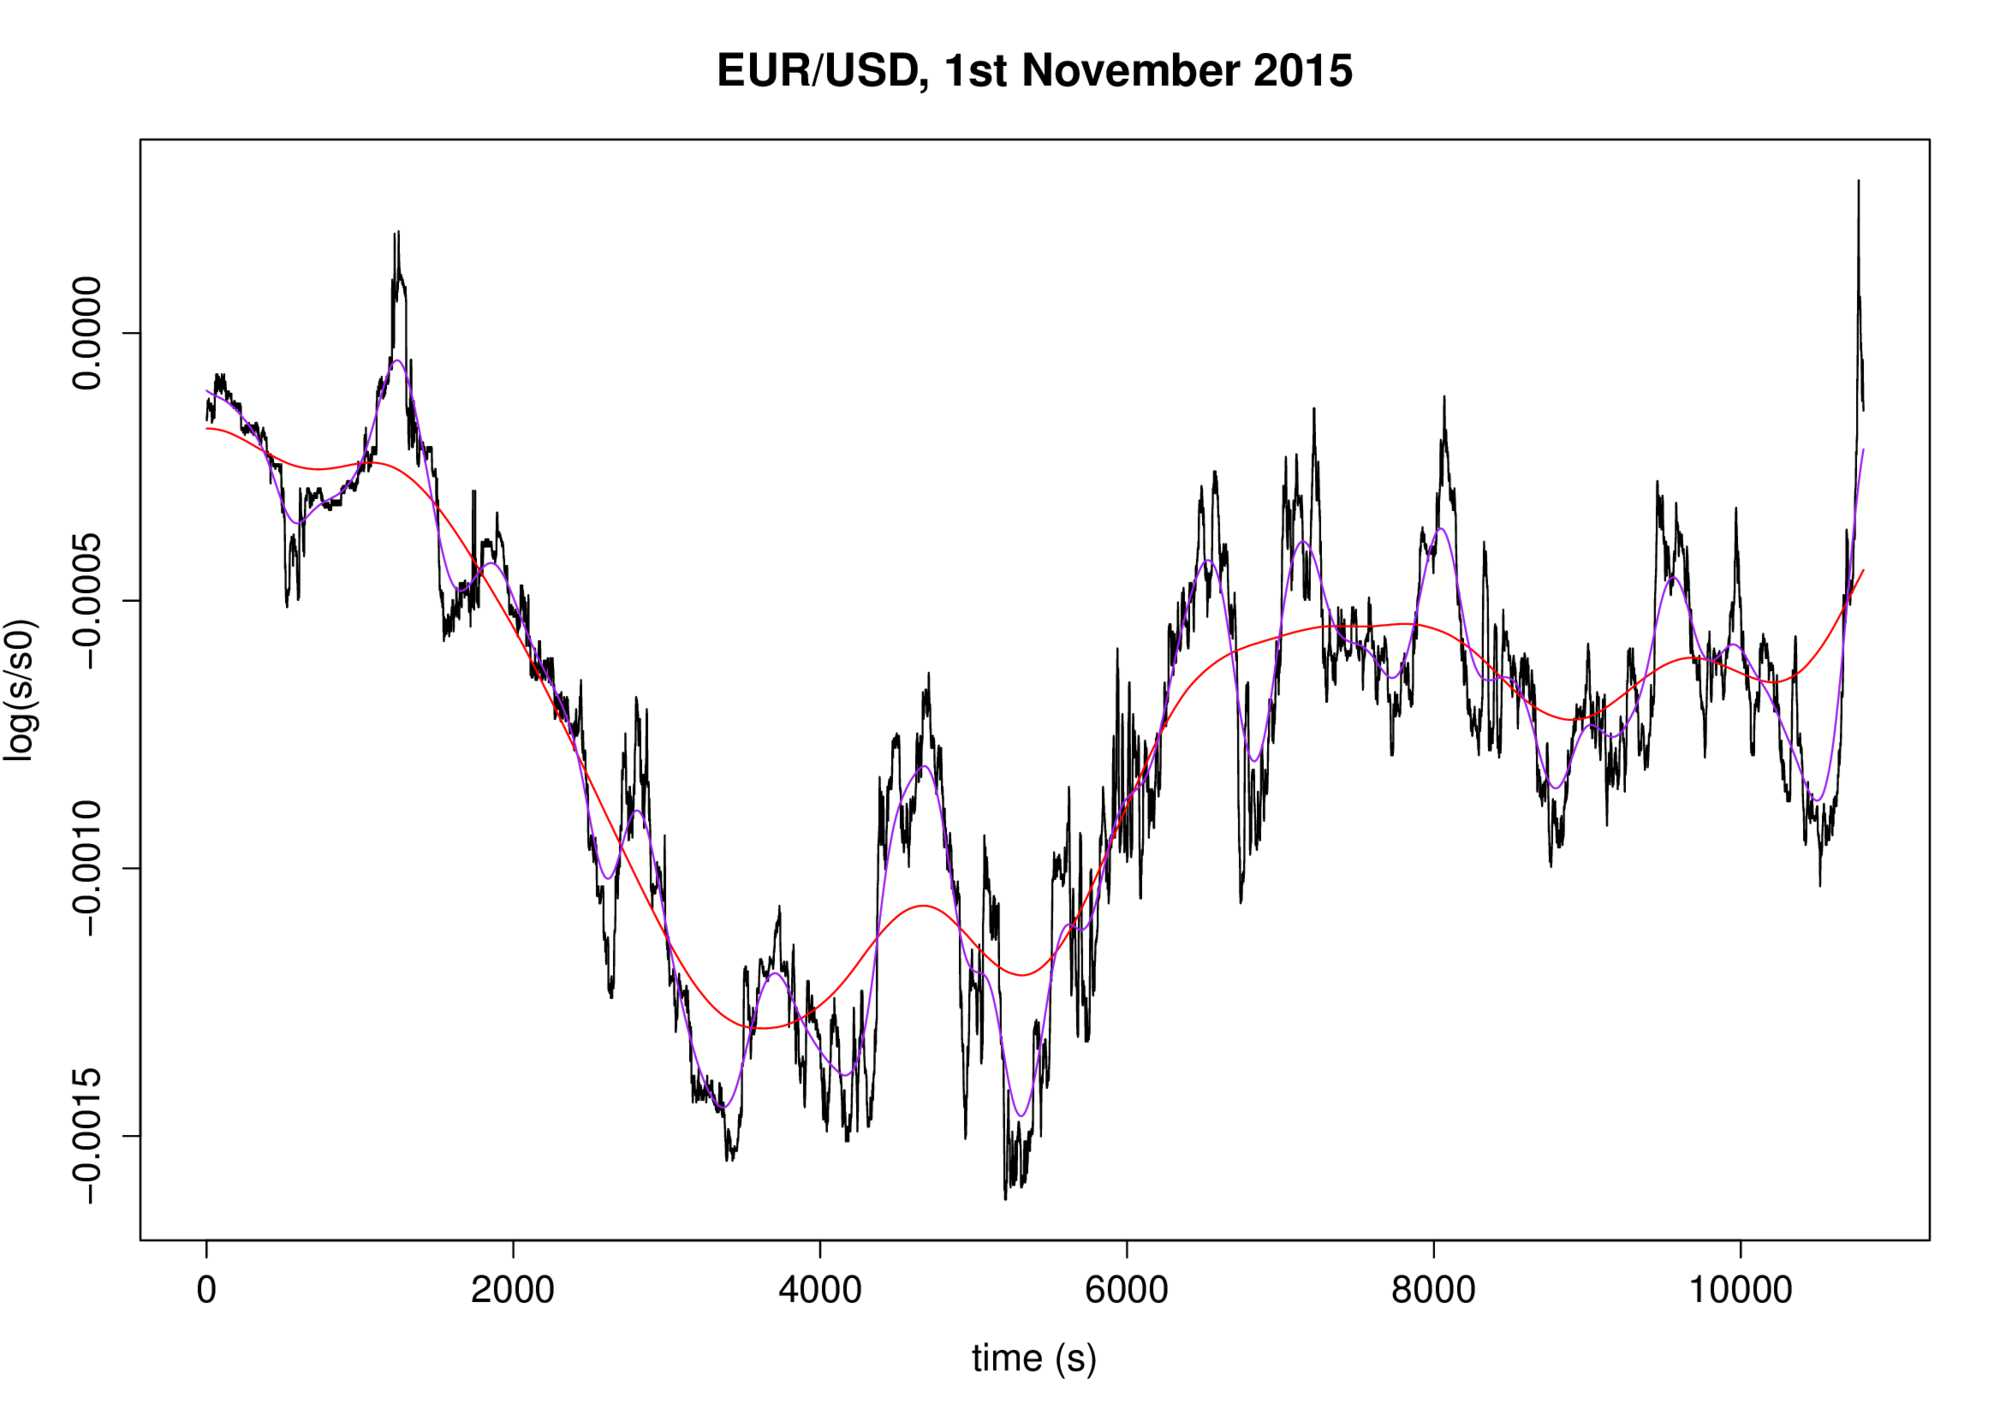
\includegraphics[width=\linewidth]{Figures/Final/C-syntheticdata-example_signal.jpg}
\appcaption{\textbf{Example of the multi-scalar structure of the signal, basis of the construction of synthetic signals | } \emph{Log-prices} are represented on a time window of around 3h for November 1st 2015 for asset EUR/USD, with 10min (purple) and 30min trends.}{\textbf{Exemple de la nature multi-scalaire des signaux.} Celle-ci est à la base de la construction des signaux synthétiques. Les \emph{log-prices} sont représentés sur une fenêtre d'environ 3h le 1er novembre 2015 pour l'actif EUR/USD, avec en violet la tendance à 10min et en rouge à 30min.\label{fig:syntheticdata:example_signal}}
\end{figure}
%%%%%%%%%%%%%%%%%%%



\bpar{
It is crucial to consider the interference between $\omega_0$ and $\omega_1$ frequencies in the reconstructed signal : correlation indeed estimated is 
\[
\rho_{e} = \rho \left[ \Delta \tilde{X}_1 , \Delta \tilde{X}_2 \right] = \rho \left[ \Delta T_1^{\omega_0} + \Delta \tilde{X}_1^{\omega} , \Delta T_2^{\omega_0} + \Delta \tilde{X}_2^{\omega}\right]
\]
what yields in the reasonable limit $\sigma_1 \gg \sigma_0$ (fundamental frequency small enough), when $\Covb{\Delta \tilde{X}_i^{\omega_1}}{\Delta X_j^{\omega}}=0$ for all $i,j,\omega_1 > \omega$ and returns centered at any scale, the correction on effective correlation due to interferences : we have at first order the expression of effective correlation

\begin{equation}
\label{eq:eff_corr}
\rho_e = \left[ \varepsilon_1 \varepsilon_2 \rho_0 + \rho \right] \cdot \left[ 1 - \frac{1}{2}\left(\varepsilon_1^2 + \varepsilon_2^2 \right) \right]
\end{equation}

{\noindent}what gives the correlation that we can effectively simulate in synthetic data.
}{
Il est crucial de noter l'interférence entre les fréquences $\omega_0$ et $\omega_1$ dans le signal construit : la correlation effectivement estimée est
\[
\rho_{e} = \rho \left[ \Delta \tilde{X}_1 , \Delta \tilde{X}_2 \right] = \rho \left[ \Delta T_1^{\omega_0} + \Delta \tilde{X}_1^{\omega} , \Delta T_2^{\omega_0} + \Delta \tilde{X}_2^{\omega}\right]
\]
ce qui conduit à dériver dans la limite raisonnable $\sigma_1 \gg \sigma_0$ (fréquence fondamentale suffisamment basse), lorsque $\Covb{\Delta \tilde{X}_i^{\omega_1}}{\Delta X_j^{\omega}}=0$ pour tous $i,j,\omega_1 > \omega$, et les retours d'espérance nulle à toutes échelles, en notant $\rho_0 = \rho \left[ \Delta T_1^{\omega_0} , \Delta T_2^{\omega_0} \right]$, $\rho = \rho \left[  \Delta \tilde{X}_1^{\omega_1} , \Delta \tilde{X}_2^{\omega_1} \right]$, et $\varepsilon_i = \frac{\sigma (\Delta T_i^{\omega_0})}{\sigma \left( \Delta \tilde{X}_i^{\omega_1}\right)}$, la correction sur la correlation effective due aux interférences : la correlation effective est alors au premier ordre

\begin{equation}
\label{eq:syntheticdata:eff_corr}
\rho_e = \left[ \varepsilon_1 \varepsilon_2 \rho_0 + \rho \right] \cdot \left[ 1 - \frac{1}{2}\left(\varepsilon_1^2 + \varepsilon_2^2 \right) \right]
\end{equation}

{\noindent}ce qui donne l'expression de la correlation que l'on pourra effectivement simuler dans les données synthétiques.
}


\bpar{
Correlation is estimated by Pearson method, with estimator for covariance corrected for bias, i.e.
\[
\hat{\rho}[X1,X2] = \frac{\hat{C}[X1,X2]}{\sqrt{\hat{\Var{}}[X1]\hat{\Var{}}[X2]}}\]
, where $\hat{C}[X1,X2] = \frac{1}{(T-1)}\sum_{t} X_1(t)X_2(t) - \frac{1}{T\cdot (T-1)} \sum_t X_1(t) \sum_t X_2(t)$ and $\hat{\Var{}}[X] = \frac{1}{T}\sum_t{X^2(t)}-\left(\frac{1}{T}\sum_tX(t)\right)^2$.
}{
La correlation est estimée par méthode de Pearson, avec l'estimateur de la covariance au biais corrigé, c'est à dire 
\[
\hat{\rho}[X1,X2] = \frac{\hat{C}[X1,X2]}{\sqrt{\hat{\Var{}}[X1]\hat{\Var{}}[X2]}}
\]
, où $\hat{C}[X1,X2] = \frac{1}{(T-1)}\sum_{t} X_1(t)X_2(t) - \frac{1}{T\cdot (T-1)} \sum_t X_1(t) \sum_t X_2(t)$ et $\hat{\Var{}}[X] = \frac{1}{T}\sum_t{X^2(t)}-\left(\frac{1}{T}\sum_tX(t)\right)^2$.
}



\bpar{
The tested predictive model $M_{\omega_1}$ is a simple \emph{ARMA} for which parameters $p=2,q=0$ are fixed (as we do not create lagged correlation, we do not expect large orders of auto-regression as these kind of processes have short memory for real data ; furthermore smoothing is not necessary as data are already filtered). It is however applied in an adaptive way\footnote{adaptation level staying low, as parameters $T_W,p,q$ and model type do not vary. We are positioned within the framework of~\cite{potiron2016estimating} which assumes a locally parametric dynamic but for which meta-parameters are fixed. We could imagine a variable $T_W$ which would adapt for the best local fit, the same way parameters are estimated in bayesian signal processing by augmentation of the state with parameters.}. More precisely, given a time window $T_W$, we estimate for any $t$ the model on $[t-T_W+1,t]$ in order to predict signals at $t+1$.
}{
Le modèle de prédiction $M_{\omega_1}$ testé est simplement un modèle \emph{ARMA} pour lequel on fixe les paramètres $p=2,q=0$ (on ne créée pas de correlation retardée, on ne s'attend donc pas à de grand ordre d'auto-regression, les signaux originaux étant à mémoire relativement courte ; de plus le lissage n'est pas nécessaire puisqu'on travaille sur des données filtrées), appliqué de manière adaptative\footnote{il s'agit d'un niveau d'adaptation relativement faible, les paramètres $T_W,p,q$ et même le type de modèle restant fixés. On se place ainsi dans le cadre de~\cite{potiron2016estimating} qui suppose une dynamique localement paramétrique, mais pour lequel on fixe les méta-paramètres de la dynamique. On pourrait imaginer estimer un $T_W$ variable qui s'adapterait pour une meilleure estimation locale, à l'image de l'estimation de paramètres en traitement du signal Bayesien effectuée via augmentation de l'état par les paramètres.}. Plus précisément, étant donné une fenêtre temporelle $T_W$, on estime pour tout $t$ le modèle sur $[t-T_W+1,t]$ afin de prédire les signaux à $t+1$.
}


\paragraph{Implementation}{Implémentation}


\bpar{
Experiments are implemented in \texttt{R} language, using in particular the \texttt{MTS}~\cite{Tsay:2015xy} library for time-series models. Cleaned data and source code are openly available on the \texttt{git} repository of the project\footnote{at \texttt{https://github.com/JusteRaimbault/SynthAsset}}. 
}{
L'implémentation est faite en language R, utilisant en particulier la bibliothèque \texttt{MTS}~\cite{Tsay:2015xy} pour les modèles de séries temporelles. Les données nettoyées et le code source sont disponibles de manière ouverte sur le dépôt \texttt{git} du projet\footnote{at \texttt{https://github.com/JusteRaimbault/SynthAsset}}.
}



\paragraph{Results}{Résultats}



\bpar{
Figure~\ref{fig:effective_corrs} gives effective correlations computed on synthetic data. For standard parameter values (for example $\omega_0=24\textrm{h}$, $\omega_1=2\textrm{h}$ and $\rho=-0.5$), we find $\rho_0\simeq 0.71$ et $\varepsilon_i \simeq 0.3$ what yields $\left| \rho_e - \rho \right|\simeq 0.05$. We observe a good agreement between observed $\rho_e$ and values predicted by~\ref{eq:eff_corr} in the interval $\rho \in [-0.5,0.5]$. On the contrary, for larger absolute values, a deviation increasing with $\left|\rho\right|$ and as $\omega_1$ decreases : it confirms the intuition that when frequency decreases and becomes closer to $\omega_0$, interferences between the two components are not negligible anymore and invalidate independence assumptions for example. 
}{
La figure~\ref{fig:syntheticdata:effective_corrs} donne les correlations effectives calculées sur les données synthétiques. Pour des valeurs standard des paramètres (par exemple pour $\omega_0=24\textrm{h}$, $\omega_1=2\textrm{h}$ et $\rho=-0.5$), on a $\rho_0\simeq 0.71$ et $\varepsilon_i \simeq 0.3$ et ainsi $\left| \rho_e - \rho \right|\simeq 0.05$. On constate dans l'intervalle $\rho \in [-0.5,0.5]$ un bon accord entre la valeur $\rho_e$ prédite par~\ref{eq:eff_corr} et les valeurs observées, et une déviation pour de plus grandes valeurs absolues, d'autant plus grande que $\omega_1$ est petit : cela confirme l'intuition que lorsque la fréquence descend et se rapproche de $\omega_0$, les interférences entre les deux composantes vont devenir non négligeables et invalider les hypothèses d'indépendance par exemple.
}


\bpar{
We apply then the predictive model described above to synthetic data, in order to study its mean performance as a function of correlation between signals. Results for $\omega_1 = 1\textrm{h},1\textrm{h}30,2\textrm{h}$ are shown in Fig.~\ref{fig:model_perf}. The a priori counter-intuitive result of a maximal performance at vanishing correlation for one of the assets confirms the role of synthetic data to better understand system mechanisms : the study of lagged correlations shows an asymmetry in the real data that we can understand at a daily scale as an increased influence of EUR/GBP on EUR/USD with a rough two hours lag. The existence of this \emph{lag} allows a ``good'' prediction of EUR/USD thanks to fundamental component. This predictive power is perturbed by added noises in a way that increases with their correlation. The more noises correlated are, the more he model will take them into account and will make false predictions because of the markovian character of simulated brownian\footnote{the model used has theoretically no predictive power at all on pure brownian}.
}{
On applique ensuite le modèle prédictif décrit ci-dessus aux données synthétiques, afin d'étudier sa performance moyenne en fonction du niveau de correlation des données. Les résultats pour $\omega_1 = 1\textrm{h},1\textrm{h}30,2\textrm{h}$ sont présentés en figure~\ref{fig:syntheticdata:model_perf}. Le résultat a priori contre-intuitif d'une performance maximale à correlation nulle pour l'un des actifs confirme l'intérêt d'une génération de données hybrides : l'étude des correlations décalées (\emph{lagged correlations}) montre une dissymétrie présente dans les données réelles, interprété à l'échelle journalière comme une influence augmentée de EURGBP sur EURUSD à 2h de décalage environ. L'existence de ce \emph{lag} permet une ``bonne'' prédiction de EURUSD due à la fréquence fondamentale, perturbée par le bruit ajouté, de façon proportionnelle à sa correlation : plus les bruits sont corrélés, plus le modèle les prendra en compte et se trompera plus à cause du caractère markovien des browniens simulés\footnote{En théorie le modèle utilisé n'a aucun pouvoir prédictif sur des browniens purs}.
}


\bpar{
This case study stays a \emph{toy-model} and has no direct practical application, but demonstrates however the relevance of using simulated synthetic data. Further developments can be directed towards the simulation of more realistic data (presence of consistent \emph{lagged correlation} patterns, more realistic models than Black-Scholes) and apply it on more operational predictive models.
}{
L'exemple présenté ici est un \emph{modèle jouet} et n'a pas d'application pratique, mais démontre l'intérêt de l'utilisation des données synthétiques simulées. On peut imaginer simuler des données plus proches de la réalité (existence de motifs réalistes de \emph{lagged correlation} par exemple, modèles plus réalistes que le Black-Scholes) et appliquer la méthode sur des modèles plus opérationnels.
}




%%%%%%%%%%%%%%%%%%%
\begin{figure}
%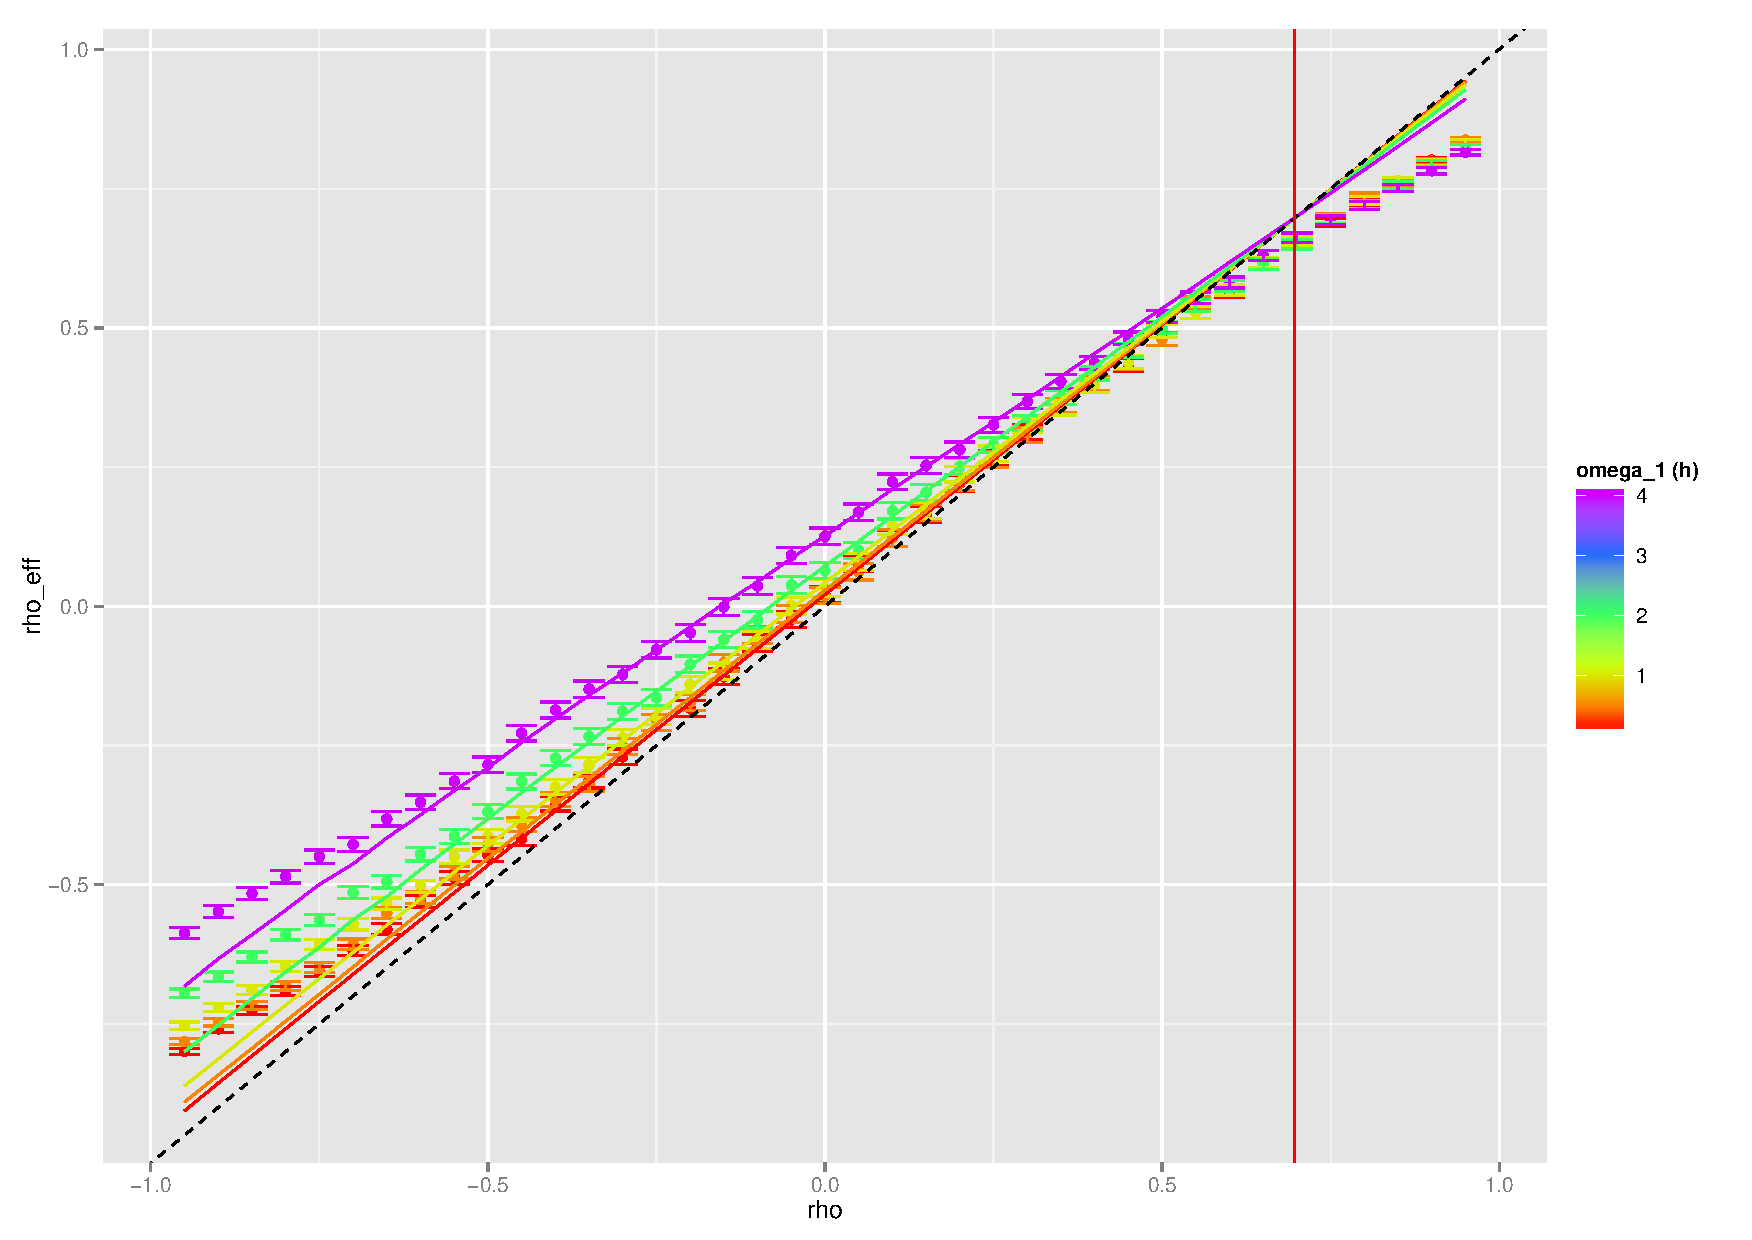
\includegraphics[width=\textwidth]{Figures/SyntheticData/effectiveCorrs_withGoodTh_A4}
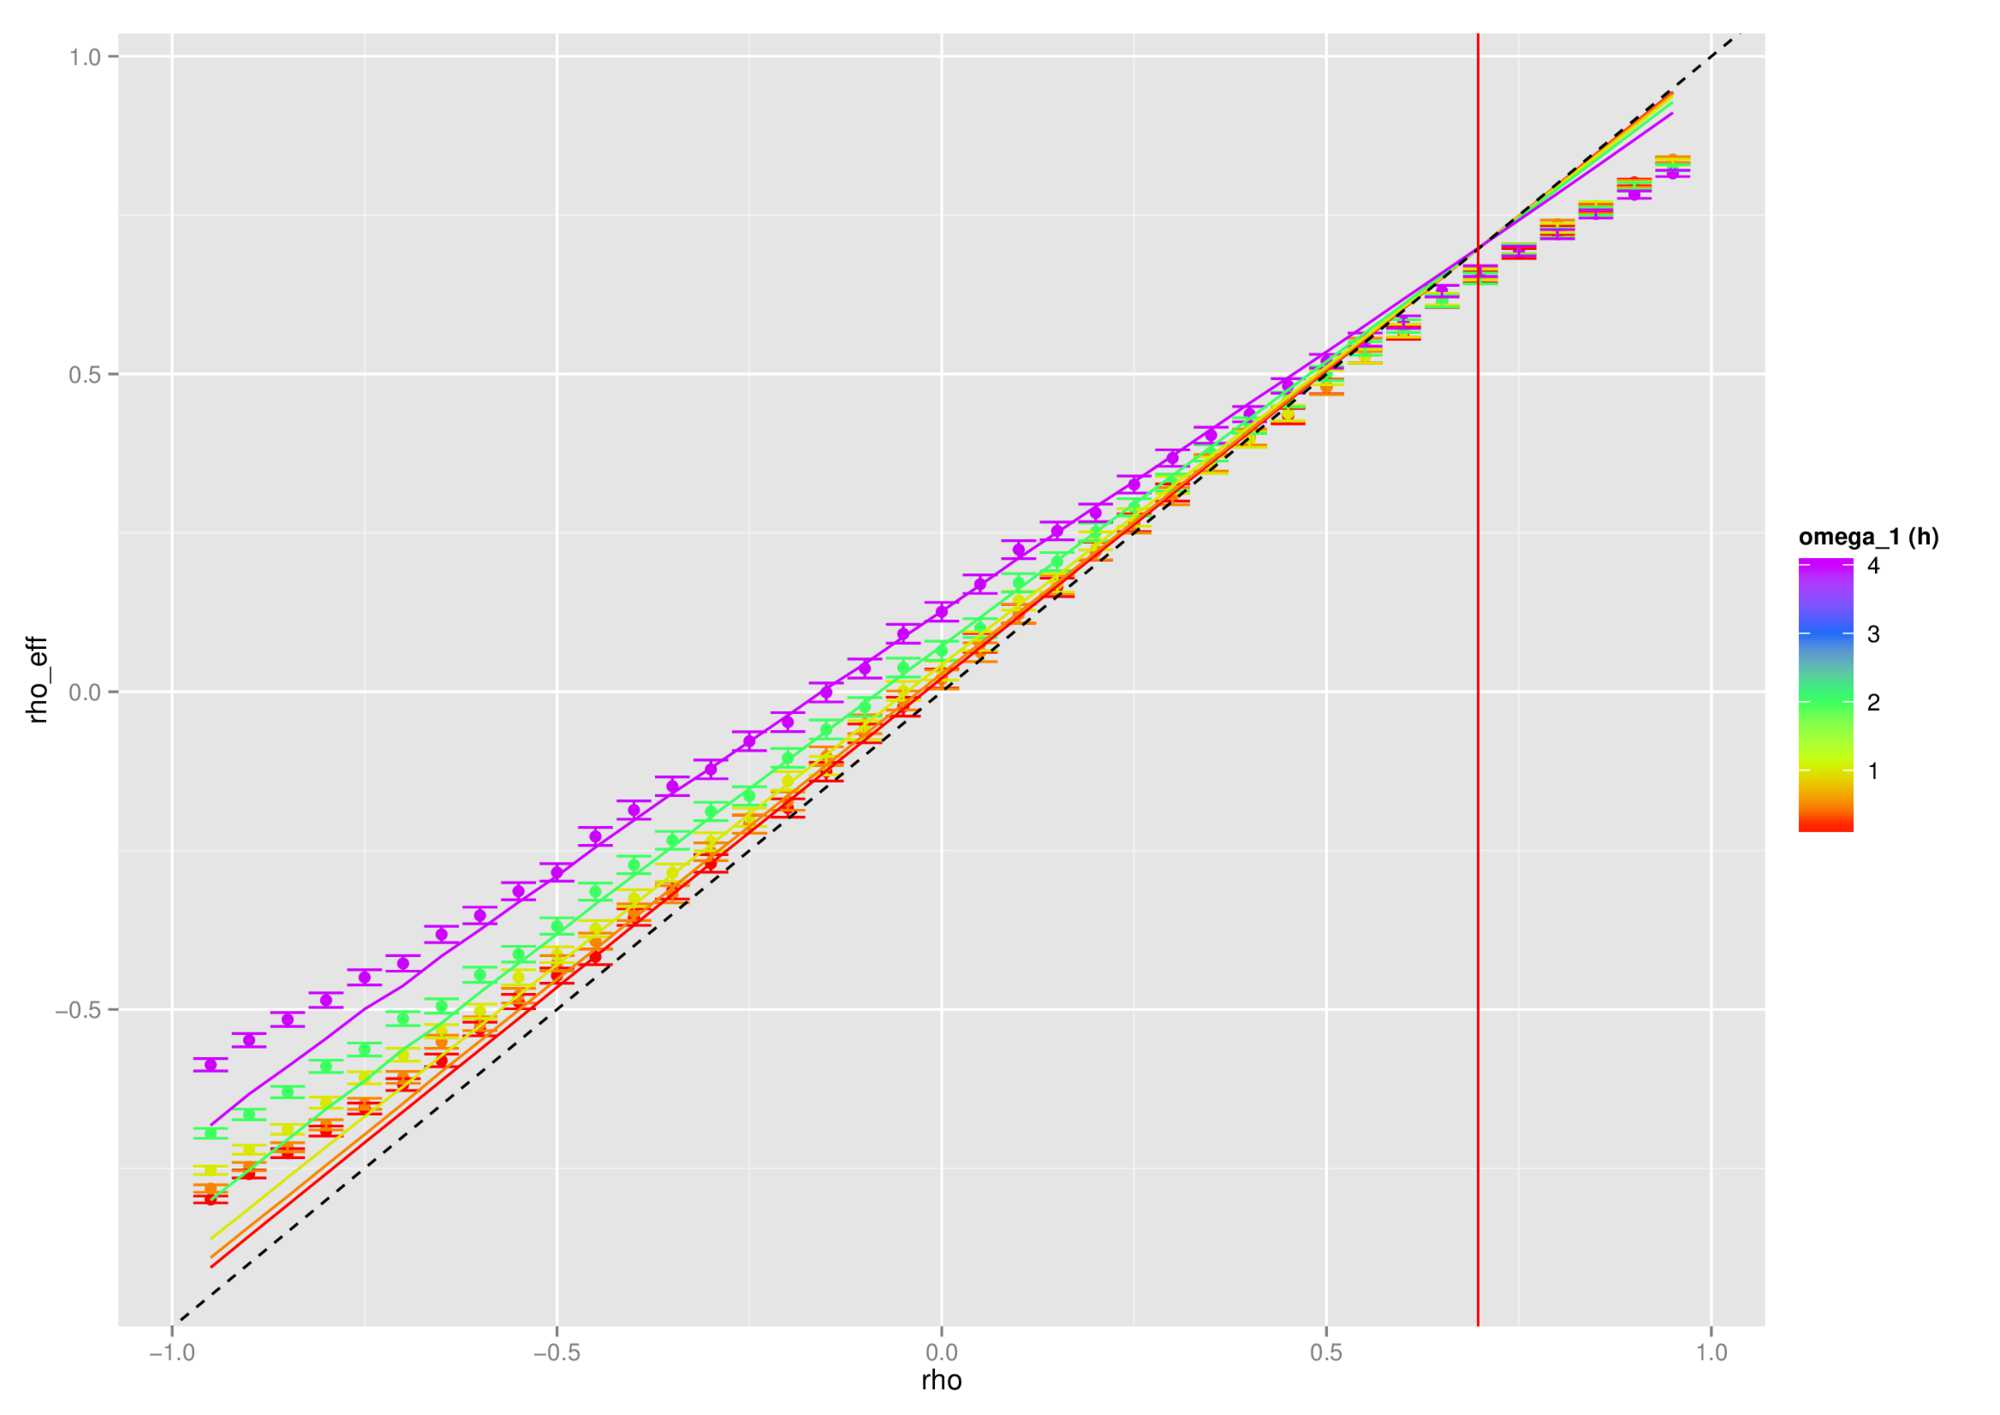
\includegraphics[width=\linewidth]{Figures/Final/C-syntheticdata-effective_corrs.jpg}
\appcaption{\textbf{Effective correlations obtained on synthetic data.} Dots represent estimated correlations on a synthetic dataset corresponding to 6 months between June and November 2015 (error-bars give 95\% confidence intervals obtained with standard Fisher method) ; scale color gives filtering frequency $\omega_1=10\textrm{min},30\textrm{min},1\textrm{h},2\textrm{h},4\textrm{h}$ ; solid lines give theoretical values for $\rho_e$ obtained by~\ref{eq:syntheticdata:eff_corr} with estimated volatilities (dotted-line diagonal for reference) ; vertical red line position is the theoretical value such that $\rho = \rho_e$ with mean values for $\varepsilon_i$ on all points. We observe for high absolute correlations values a deviation from corrected values, what should be caused by non-verified independence and centered returns assumptions. Asymmetry is caused by the high value of $\rho_0 \simeq 0.71$.}{\textbf{Corrélations Effectives obtenues sur données synthétiques.} Les points donnents les corrélations estimées sur un jeu de données synthétiques basé sur 6 mois entre juin et novembre 2015 (les barres d'erreur donnent les intervalles de confiance à 95\% obtenus par méthode de Fisher standard) ; l'échelle de couleur donne la fréquence de filtrage $\omega_1=10\textrm{min},30\textrm{min},1\textrm{h},2\textrm{h},4\textrm{h}$ ; les lignes pleines donnent les valeurs théoriques obtenues par l'équation~\ref{eq:syntheticdata:eff_corr} avec les volatilités estimées (la diagonale en pointillé donne la référence) ; la ligne verticale rouge est à la position de la valeur théorique telle que $\rho = \rho_e$ avec les valeurs moyennes de $\varepsilon_i$ sur l'ensemble des points. Nous observons pour les fortes valeurs de corrélations absolues une déviation des valeurs corrigées, qui devrait être dues à la non-vérification des hypothèses d'indépendance et de centrage des retours. L'asymétrie est due à la forte valeur de $\rho_0 \simeq 0.71$.\label{fig:syntheticdata:effective_corrs}}
\end{figure}
%%%%%%%%%%%%%%%%%%%


%%%%%%%%%%%%%%%%%%%
\begin{figure}
%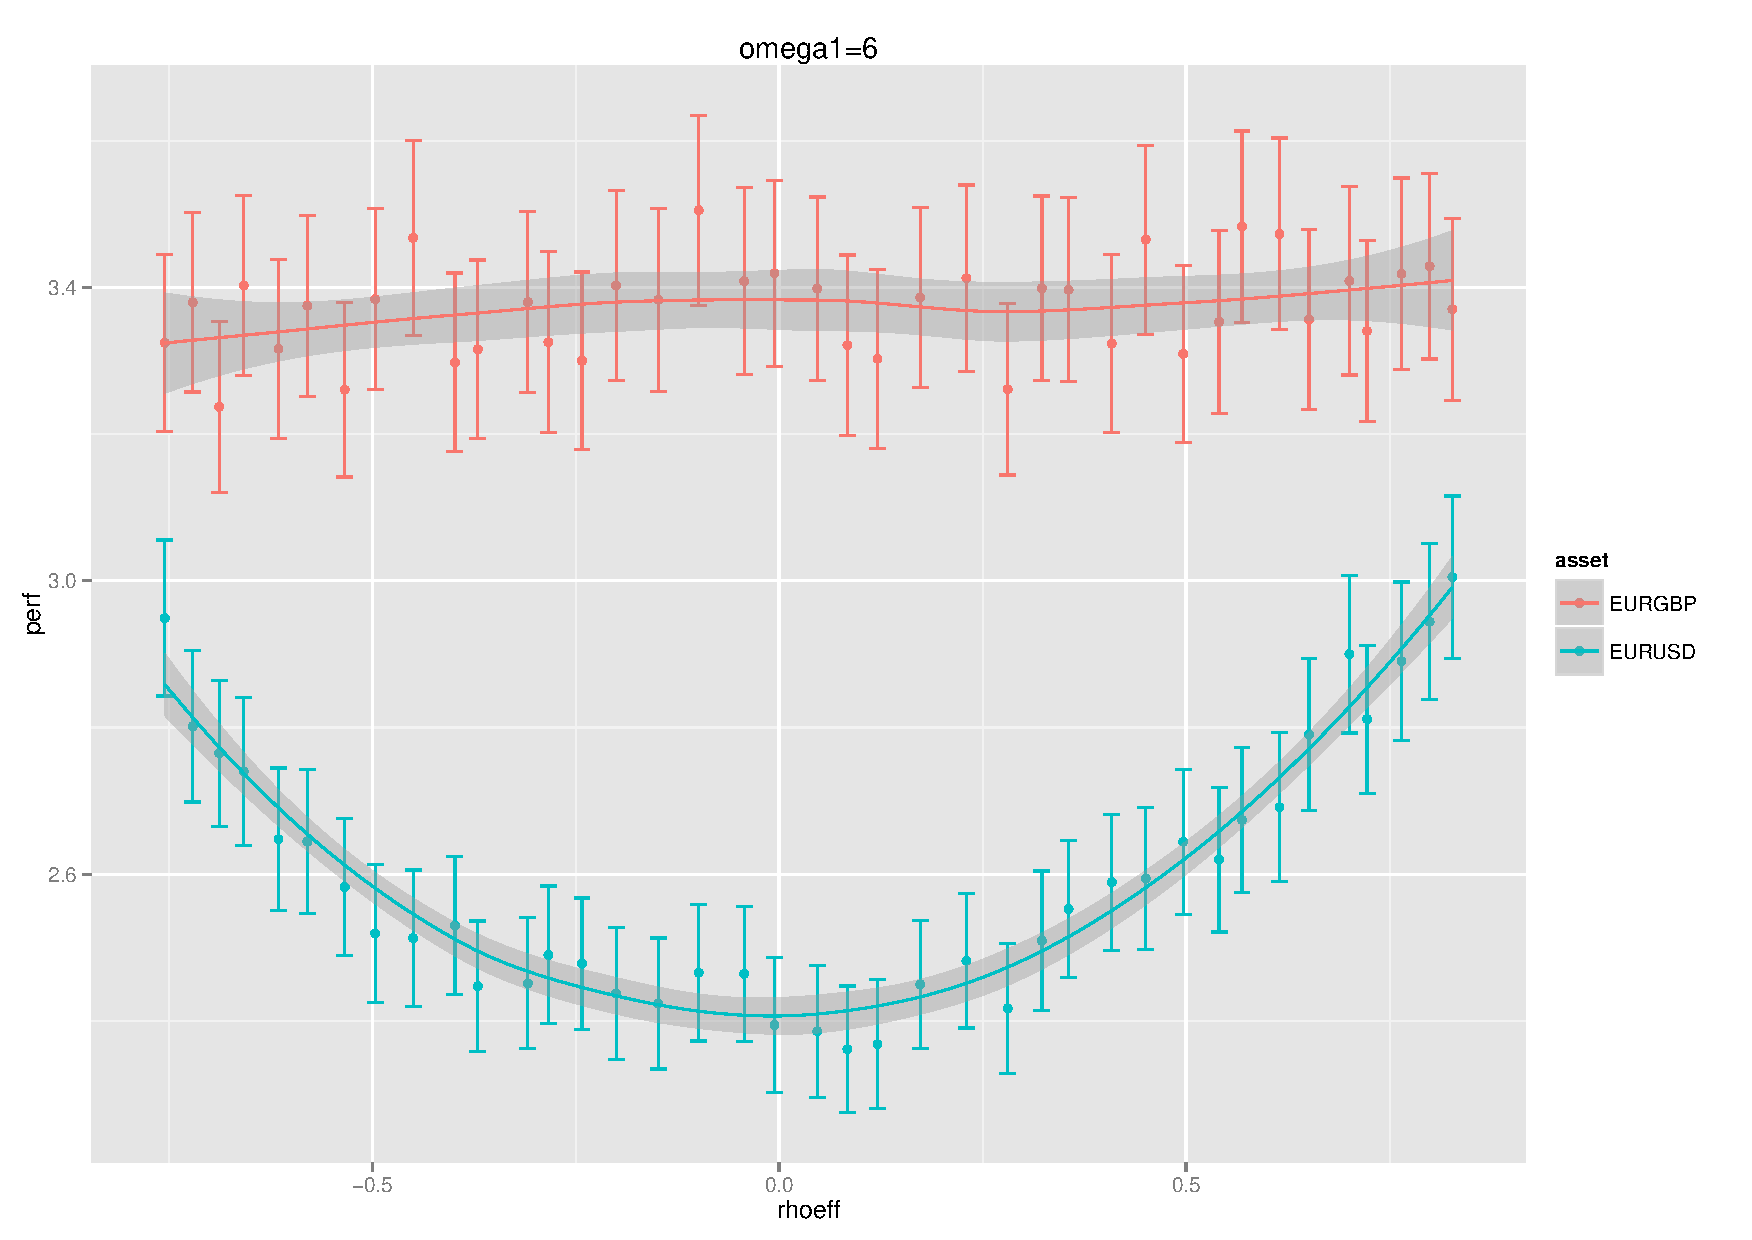
\includegraphics[width=0.48\textwidth,height=0.16\textheight]{Figures/SyntheticData/pred_filt6}
%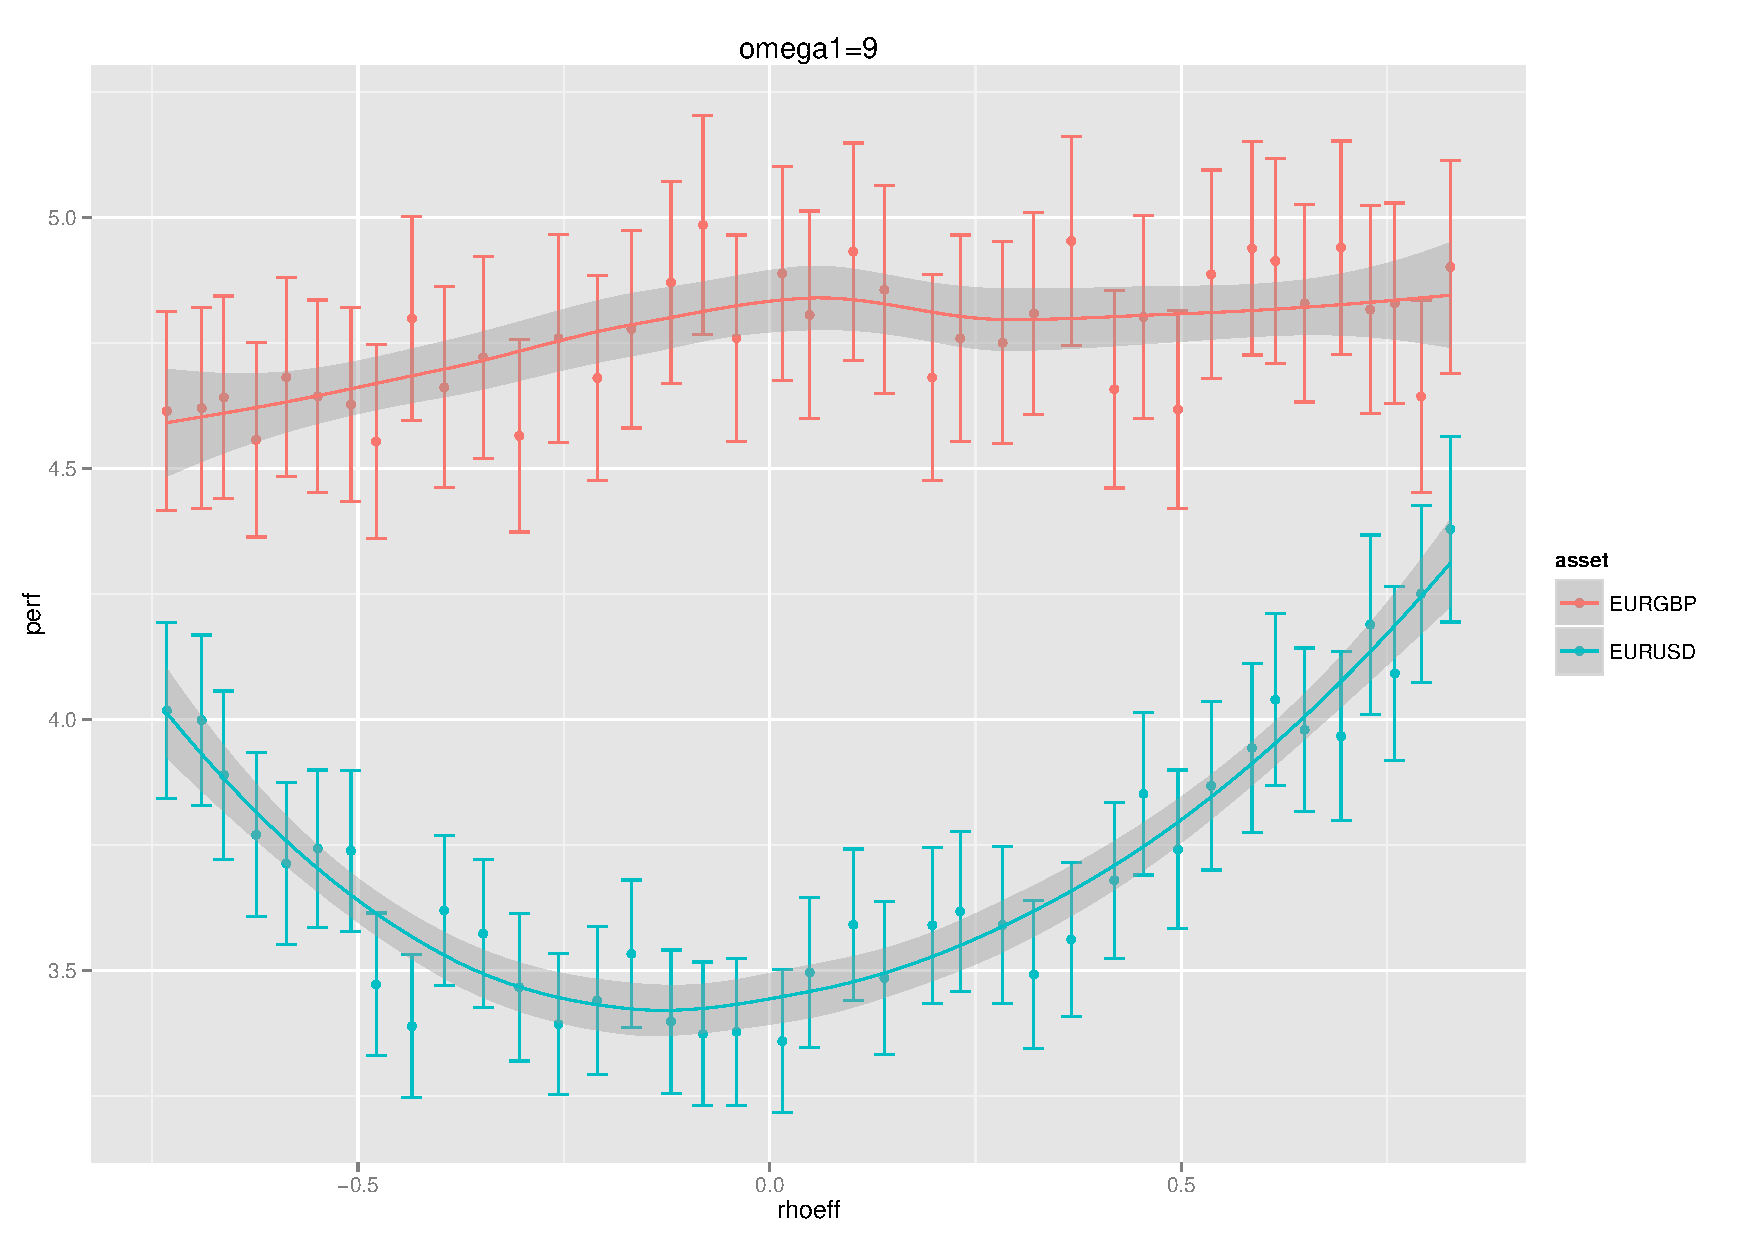
\includegraphics[width=0.48\textwidth,height=0.16\textheight]{Figures/SyntheticData/pred_filt9}\\
%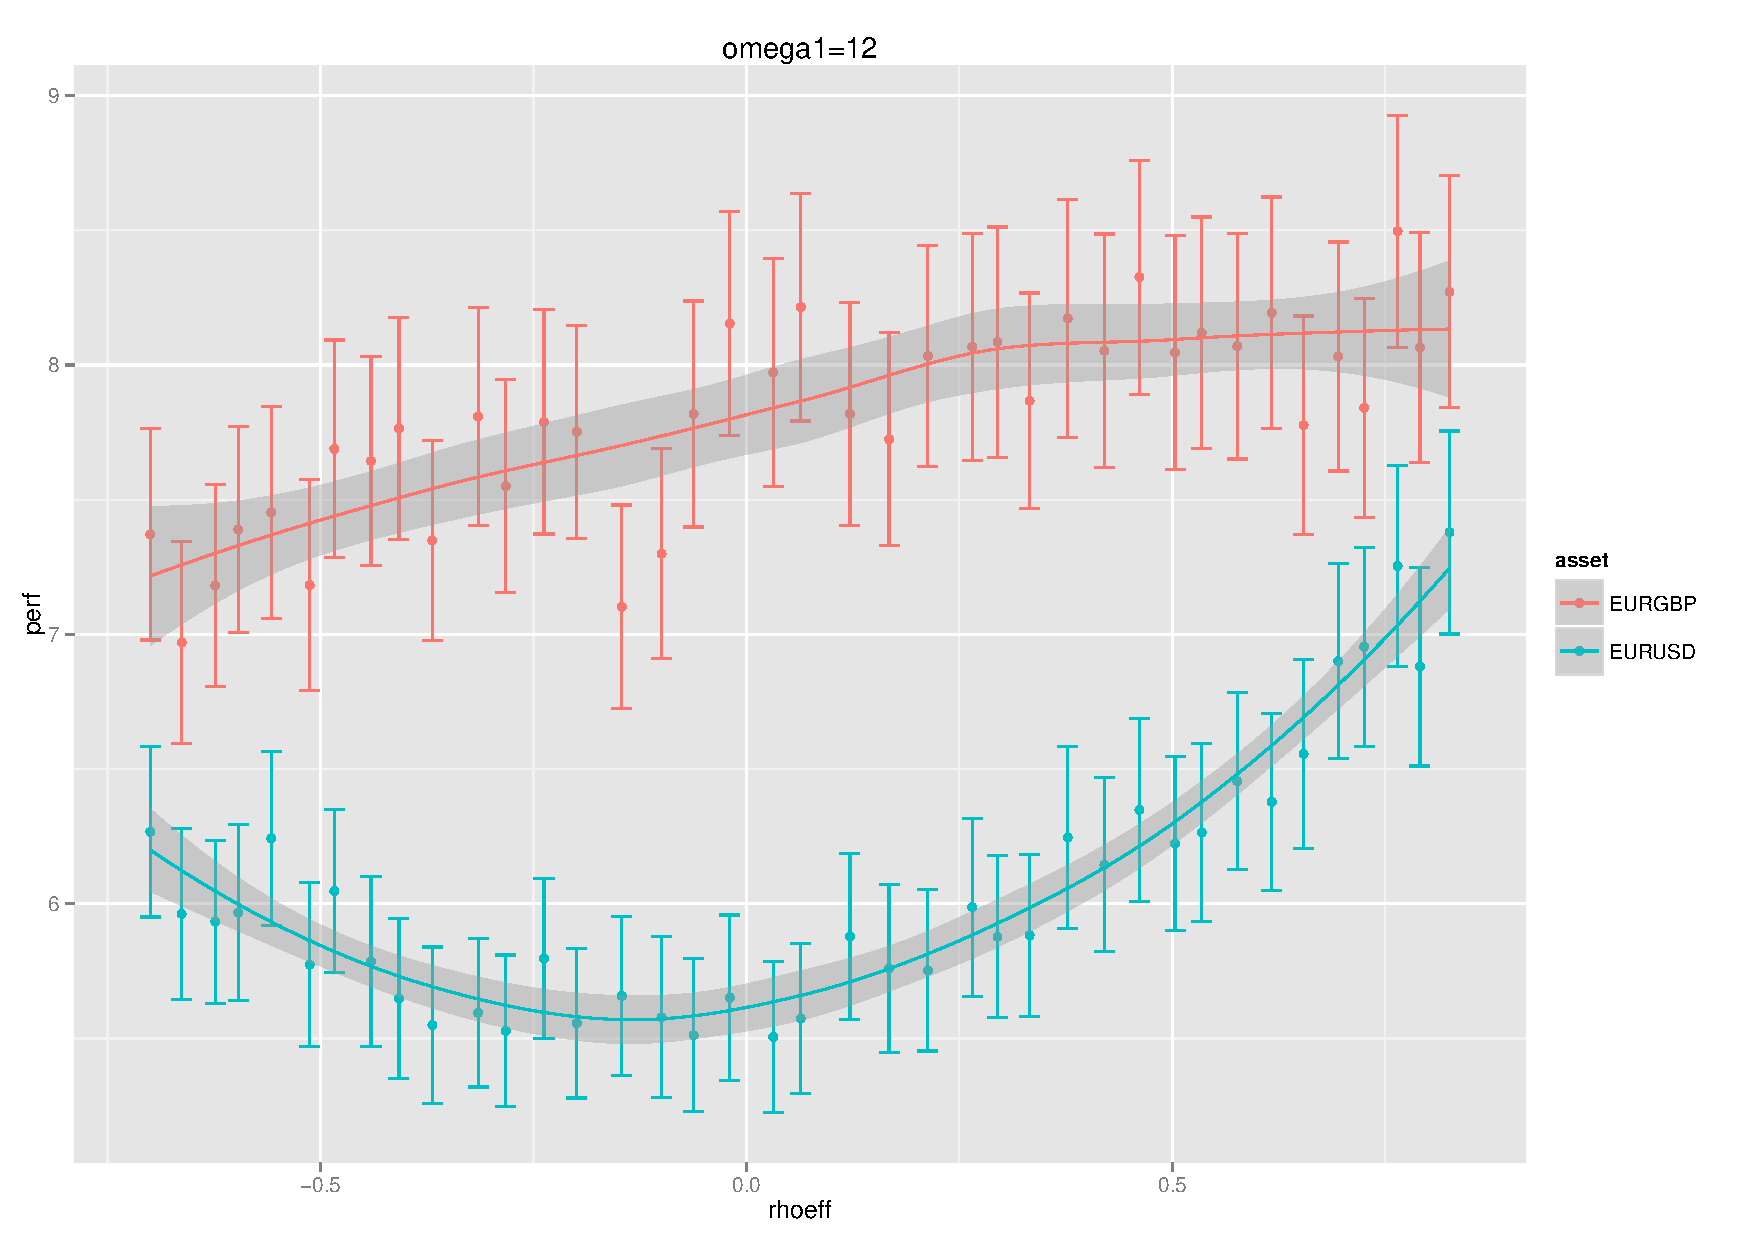
\includegraphics[width=0.48\textwidth,height=0.16\textheight]{Figures/SyntheticData/pred_filt12}
%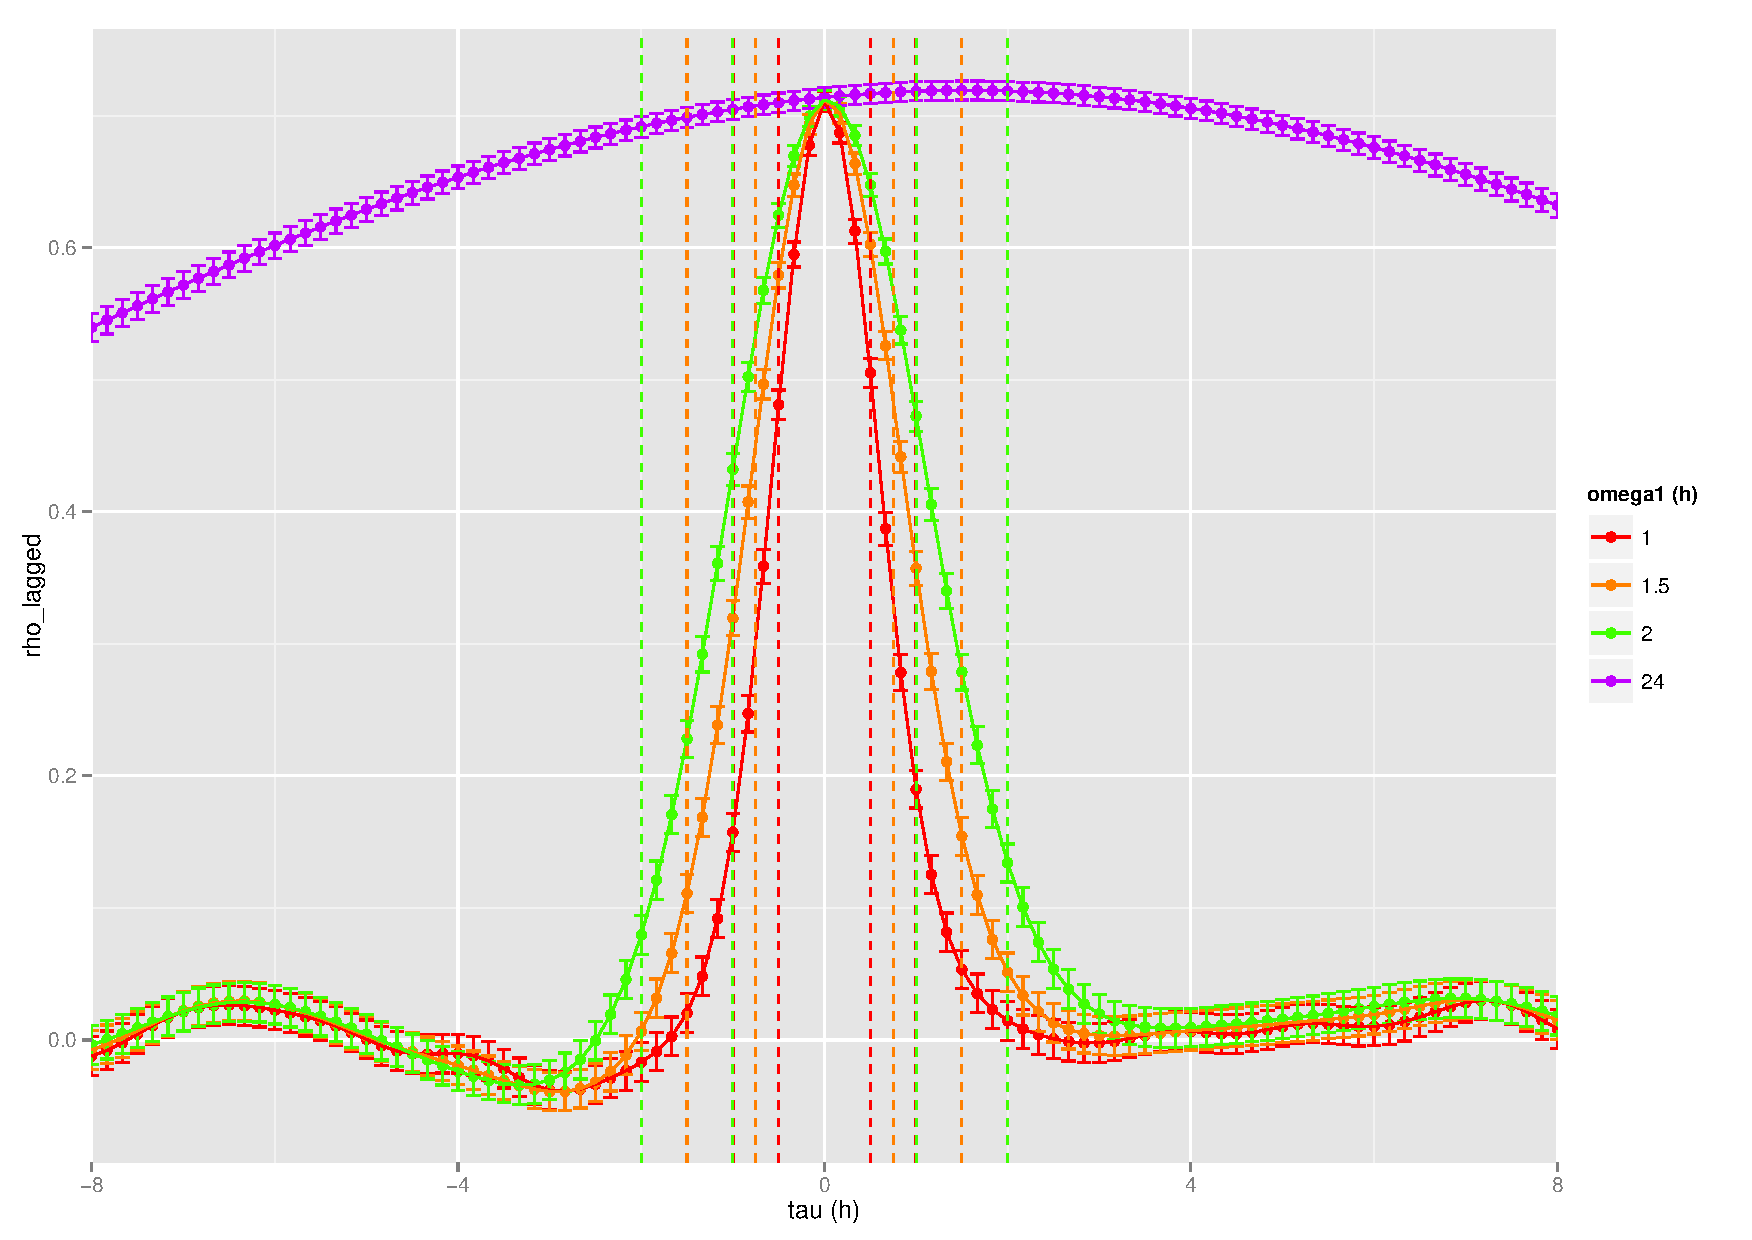
\includegraphics[width=0.48\textwidth,height=0.16\textheight]{Figures/SyntheticData/lagged_corrs}
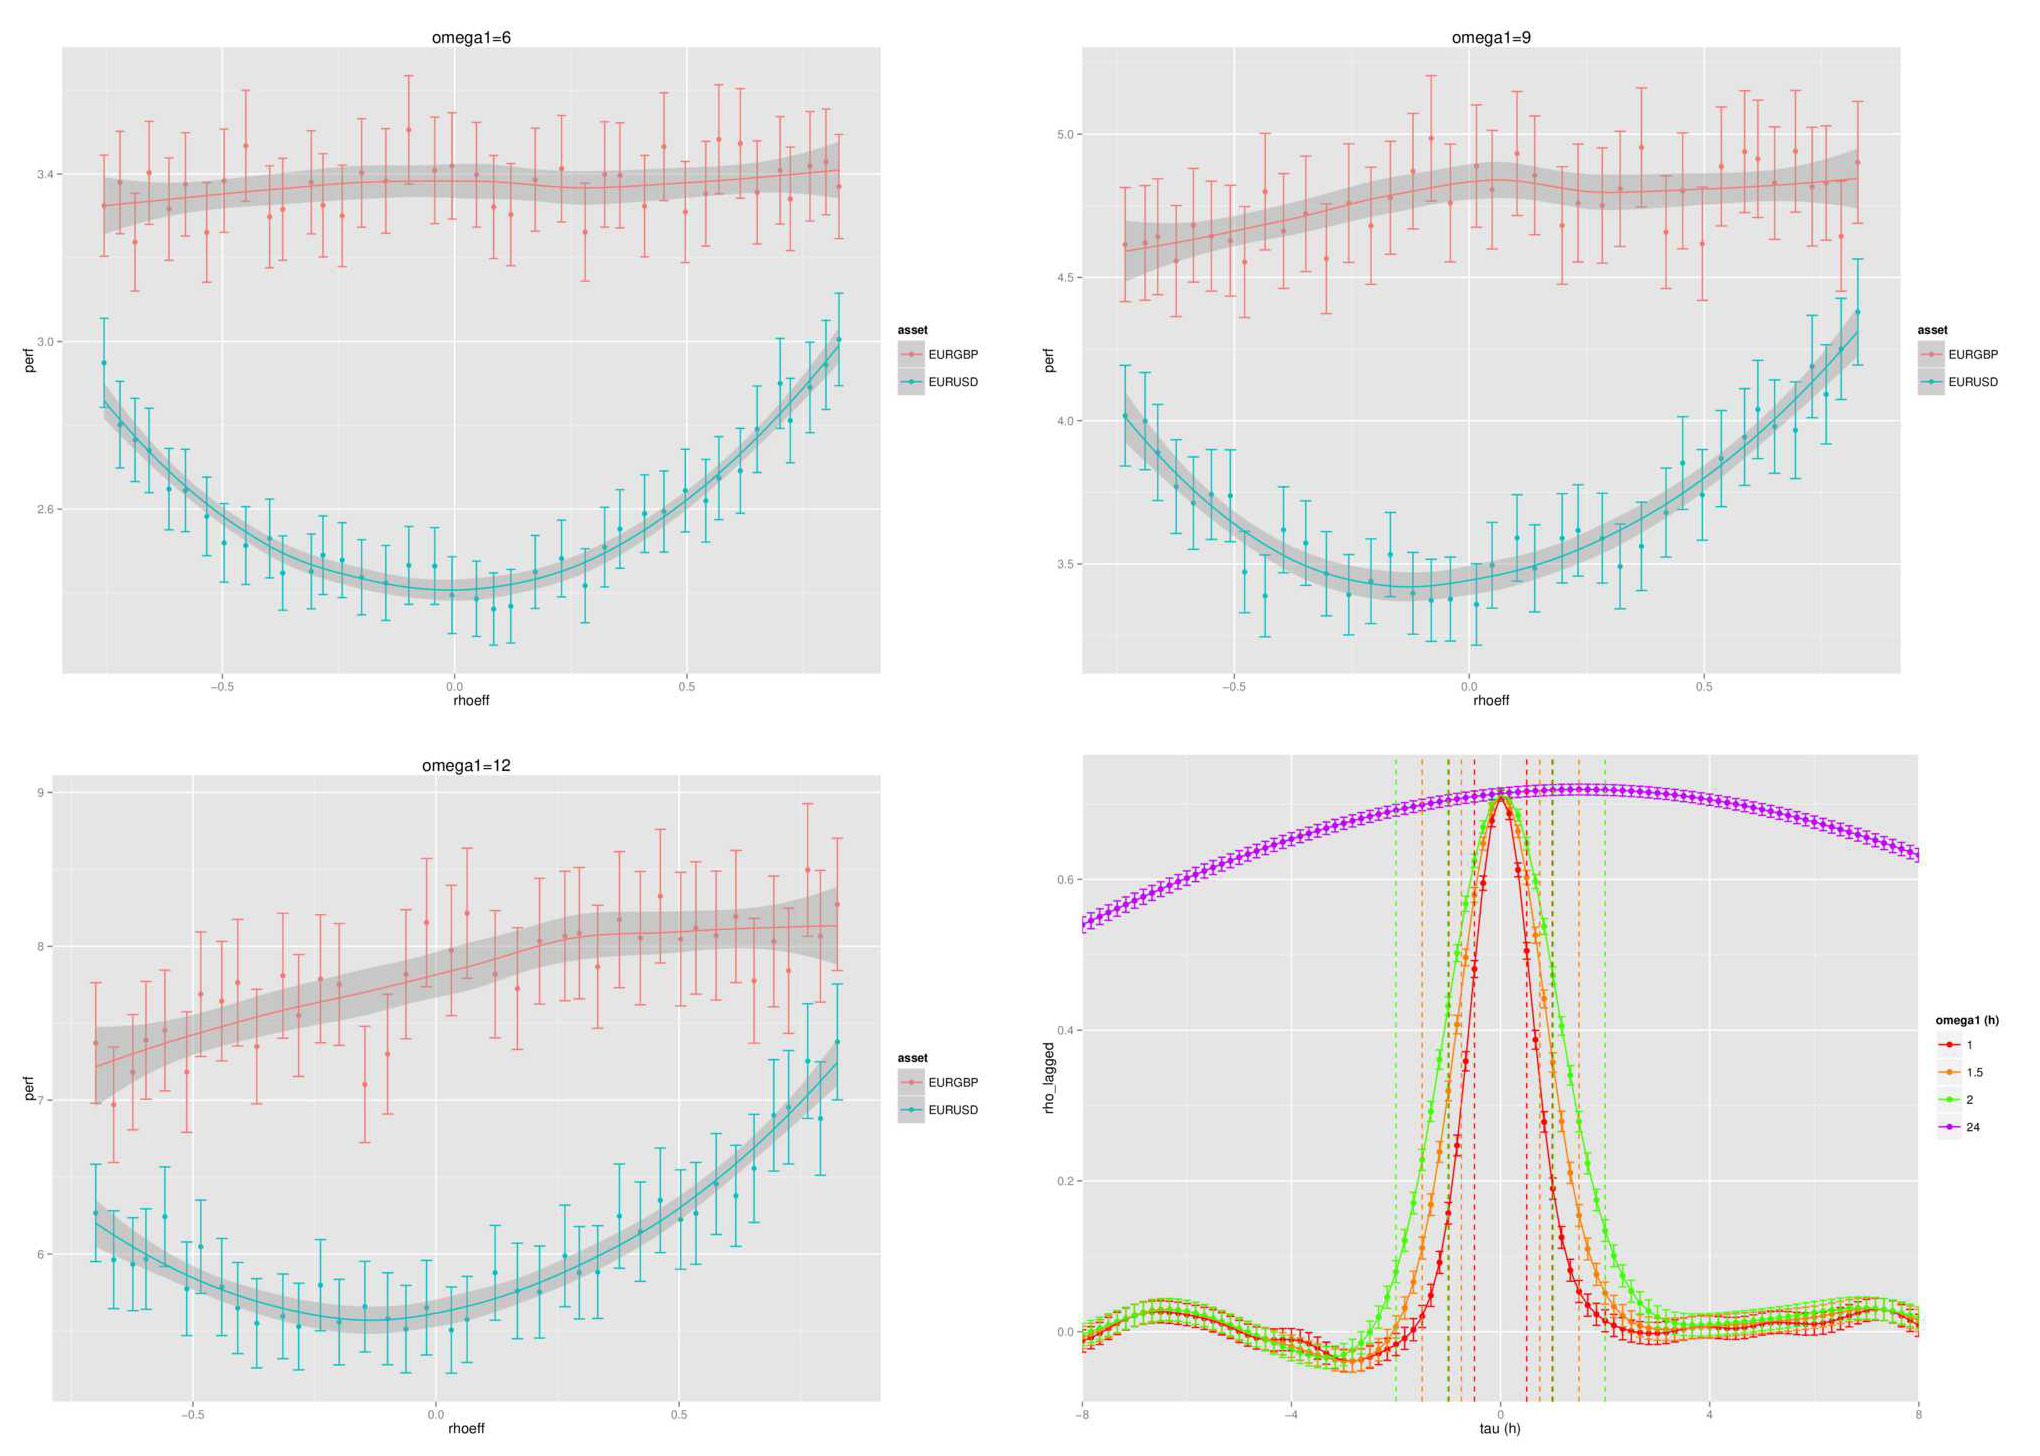
\includegraphics[width=\linewidth]{Figures/Final/C-syntheticdata-model_perf.jpg}
\appcaption{\small \textbf{Performance of a predictive model as a function of simulated correlations.} From left to right and top to bottom, three first graphs show for each asset the normalized performance of an ARMA model ($p=2,q=0$), defined as $\pi = \left(\frac{1}{T}\sum_t\left(\tilde{X}_i(t) - M_{\omega_1}\left[\tilde{X}_i\right](t)\right)^2 \right) / \sigma \left[ \tilde{X}_i \right]^2$ (95\% confidence intervals computed by $\pi = \bar{\pi} \pm (1.96\cdot \sigma [\pi])/\sqrt{T}$, local polynomial smoothing to ease reading). It is interesting to note the U-shape for EUR/USD, due to interference between components at different scales. Correlation between simulated noises deteriorates predictive power. The study of \emph{lagged correlations} (here $\rho [\Delta X_{\textrm{EURUSD}}(t),\Delta X_{\textrm{EURGBP}}(t-\tau)]$) on real data clarifies this phenomenon : fourth graph show an asymmetry in curves at any scale compared to zero lag $(\tau = 0)$ what leads fundamental components to increase predictive power for the dollar, amelioration then perturbed by correlations between simulated components. Dashed lines show time steps (in equivalent $\tau$ units) used by the ARMA at each scale, what allows to read the corresponding lagged correlation on fundamental component.}{\textbf{Performance d'un modèle prédictif en fonction des corrélations simulées.} De gauche à droite et de haut en bas, les trois premier graphes donnent pour chaque actif la performance normalisée d'un modèle ARMA ($p=2,q=0$), définie par $\pi = \left(\frac{1}{T}\sum_t\left(\tilde{X}_i(t) - M_{\omega_1}\left[\tilde{X}_i\right](t)\right)^2 \right) / \sigma \left[ \tilde{X}_i \right]^2$ (intervalles de confiance à 95\% calculés par $\pi = \bar{\pi} \pm (1.96\cdot \sigma [\pi])/\sqrt{T}$, le lissage polynomial local est pour l'aide à la lecture). Il est intéressant de noter la forme de U pour EUR/USD, due aux interférences entre composantes à différentes échelles. La corrélation entre les bruits simulés détériore le pouvoir de prédiction. L'étude des corrélation retardées (ici données par $\rho [\Delta X_{\textrm{EURUSD}}(t),\Delta X_{\textrm{EURGBP}}(t-\tau)]$) sur les données réelles clarifie ce phénomène : le quatrième graphe présente une asymétrie des courbes à toutes les échelles par rapport au décalage nul $(\tau = 0)$ ce qui conduit les composantes fondamentales à accroitre le pouvoir prédictif pour le dollar, amélioration qui est ensuite perturbée par les corrélations entre les composantes simulées. Les lignes pointillées donnent les pas de temps (en équivalent en unités de $\tau$) utilisés par les ARMA à chaque échelle, ce qui permet de lire la corrélation retardée correspondante sur les composantes fondamentales.\label{fig:syntheticdata:model_perf}}
\end{figure}
%%%%%%%%%%%%%%%%%%%








%%%%%%%%%%%%%%%%%%


% TODO : include other projects ? MigrationDynamics : yes if mentioned in perspectives





%%%%%%%%%%%%%%%%%%
%% Appendix : reflexivity
%  -> should also include reading graph / possible paths

% Chapter 

\chapter{Quantitative Analysis of Thesis reflexivity}{Quantitative Analysis of Thesis reflexivity} % Chapter title

\label{app:reflexivity} % For referencing the chapter elsewhere, use \autoref{ch:name} 

%----------------------------------------------------------------------------------------


% TODO : compare to semantic network of concepts in Gödel Escher Bach.

%%%%%%%%%%%%%%%%%%


%%%%%%%%%%%%%%%%%%
%% Appendix : datasets
%\chapter{Datasets}{Données} % Chapter title
\chapter{Données}

\markboth{\thechapter\space Données}{\thechapter\space Données}


\label{app:data} % For referencing the chapter elsewhere, use \autoref{ch:name} 

%----------------------------------------------------------------------------------------


%\headercit{}{}{}

%when possible, specify data citation (ex. traffic data : TransportationEquilibrium paper) ; try to put all on dataverse ; laius sur dataverse, partage des données etc.



\bpar{
This appendix lists and describes the different open datasets created and used in the thesis.
}{
Cette annexe liste et décrit les différents jeux de données ouvertes que nous avons été amenés à créer et à utiliser dans la thèse. Les données sont en effet bien un domaine de connaissance propre, et les opérations de collecte et de consolidation sont une étape scientifique à part entière.
}





%%%%%%%%%%%%%%
\section{Grand Paris Traffic Data}{Données de Traffic du Grand Paris}

% données syntadin : checker la licence

\subsection{Specification}{Spécification}

\paragraph{Citation}{Citation}

\paragraph{Type and Format}{Type et Format}

\paragraph{License}{Licence}

\paragraph{Availability}{Disponibilité}


\subsection{Description}{Description}




%%%%%%%
%% -- ON HOLD --
% (clarifier degré d'ouverture possible 


%%%%%%%%%%%%%%
%\section{US Gaz Prices}{Prix de l'Essence aux Etats-Unis}


%\subsection{Specification}{Spécification}

%\paragraph{Citation}{Citation}

%\paragraph{Type and Format}{Type et Format}

%\paragraph{License}{Licence}

%\paragraph{Availability}{Disponibilité}

%\subsection{Description}{Description}







%%%%%%%%%%%%%%
\section{Topological Road Network}{Graphes topologiques des Réseaux Routiers}

La simplification des réseaux routiers, opérée à grande échelle pour l'Europe et la Chine sur les données d'OpenStreetMap, produit les graphes topologiques correspondants. 


\subsection{Description}{Description}




\subsection{Specification}{Spécification}

\paragraph{Citation}{Citation} 

Raimbault, Juste, 2018, "Simplified road networks, Europe and China", doi:10.7910/DVN/RKDZMV, Harvard Dataverse, V1

\paragraph{Type and Format}{Type et Format}

Edge lists of graphs. Format : postgis dumps

\paragraph{License}{Licence}

CC0

\paragraph{Availability}{Disponibilité}

La base est disponible sur le Harvard Dataverse à \url{http://dx.doi.org/10.7910/DVN/RKDZMV}.




%%%%%%%%%%%%%%
%% ON HOLD

%\section{French Freeway Dynamical Network}{Réseau Dynamique des Autoroutes Françaises}

%\comment{Merger avec la base bassin parisien de Florent, faire un data paper.}
%  -> dans une autre vie !





%%%%%%%%%%%%%%
\section{Interviews}{Interviews}

\label{app:sec:interviews}

% laius sur pourquoi données "quali" devraient pas être plus dispo (quand accord intervié) ; outils idem ex. git, dissocié quanti : cf exemple galère excel notes ridicule, refus systématique et catégorique d'une alternative stable et fiable...

Un matériau de recherche qui serait plus ``qualitatif'' au sens classique, n'a pas de raison d'être moins ouvert que des bases de données ``quantitatives''. Dans le cas d'entretiens, l'ouverture des retranscriptions est essentielle pour la reproductibilité puisqu'il s'agit du dernier (et du premier) stade avant la traduction non reproductible en interprétations. Nous pensons également qu'elle est cruciale pour exploiter l'ensemble de leur potentiel, l'ouverture permettant leur réutilisation et donc possiblement réactions ou débats.


\subsection{Description}{Description}

\subsubsection{Interview with Denise Pumain, 2017/03/31}{Entretien avec Denise Pumain, 2017/03/31}

Cet entretien est intervenu dans le contexte d'une collecte de matériau empirique pour la rédaction de~\cite{raimbault2017applied}, qui a permis entre autre la construction du cadre de connaissances développé en~\ref{sec:knowledgeframework}. L'entretien est principalement centré sur la genèse de la Théorie Evolutive des Villes.

\subsubsection{Interview with Romain Reuillon, 2017/04/11}{Entretien avec Romain Reuillon, 2017/04/11}

Cet entretien intervient dans le même contexte, en cherchant à apporter un éclairage du point de vue des méthodes et outils. Il retrace en particulier la genèse d'OpenMole.

\subsubsection{Interview with Clémentine Cottineau, 2017/05/05}{Entretien avec Clémentine Cottineau, 2017/05/05}

Géographe à l'interface interdisciplinaire




\subsubsection{Interview with Denise Pumain, 2017/12/15}{Entretien avec Denise Pumain, 2017/12/15}

Effets structurants des infrastructures de transport et co-évolution, du point de vue de la géographie.




\subsubsection{Interview with Alain Bonnafous, 2018/01/09}{Entretien avec Alain Bonnafous, 2018/01/09}



Effets structurants des infrastructures de transport, du point de vue de l'économie des transports.



\subsection{Specification}{Spécification}

\paragraph{Citation}{Citation}

\paragraph{Type and Format}{Type et Format}

Données textuelles : transcription des entretiens au format texte.

\paragraph{License}{Licence}

% 

\paragraph{Availability}{Disponibilité}

Dépôt git : \url{https://github.com/JusteRaimbault/Entretiens}








%%%%%%%%%%%%%%
\section{Synthetic Data and simulation results}{Données Synthétiques et résultats de simulations}

Les résultats de calculs ou de simulations utilisés pour l'ensemble des résultats présentés sont disponibles de manière ouverte, soit sur le dépôt git soit sur un dépôt dataverse dédié dans le cas d'articles autonomes ou de fichiers massifs. Les liens sont les suivants pour les dépôts particuliers :

\begin{itemize}
	\item Résultats de l'exploration du corpus Cybergeo \url{http://dx.doi.org/10.7910/DVN/VU2XKT} ; Epistémologie quantitative et modélographie \url{https://github.com/JusteRaimbault/CityNetwork/tree/master/Models/QuantEpistemo/HyperNetwork/data}
	\item Indicateurs morphologiques et topologiques pour l'Europe et la Chine \url{http://dx.doi.org/10.7910/DVN/RHLM5Q}
	\item Simulation de données synthétiques par le modèle RBD pour l'identification de régimes de causalité spatio-temporelle \url{http://dx.doi.org/10.7910/DVN/KGHZZB}
	\item Simulation et calibration du modèle macroscopique d'interactions \url{}
	\item Simulation et calibration du modèle de morphogenèse pour la densité \url{http://dx.doi.org/10.7910/DVN/WSUSBA}
	\item Simulations du modèle de co-évolution macroscopique \url{http://dx.doi.org/10.7910/DVN/TYBNFQ} et \url{https://github.com/JusteRaimbault/CityNetwork/tree/master/Models/MacroCoevol/MacroCoevol/calibres} pour la calibration
	\item Simulations du modèle de co-évolution mesoscopique \url{http://dx.doi.org/10.7910/DVN/OBQ4CS}
	\item Simulations du modèle Lutecia \url{http://dx.doi.org/10.7910/DVN/V3KI2N}
\end{itemize}














%%%%%%%%%%%%%%%%%%


%%%%%%%%%%%%%%%%%%
%% Appendix : Softwares and Packages
\chapter{Softwares and Packages}{Softwares and Packages} % Chapter title

\label{app:packages} % For referencing the chapter elsewhere, use \autoref{ch:name} 

%----------------------------------------------------------------------------------------


\headercit{}{}{}



This appendix lists and describes the different open datasets created and used in the thesis.


\section{largeNetwoRk: Network Import and simplification for R}{largeNetwoRk : Import de réseau et simplification pour R}



\section{Scientific Corpus Mining}{Fouille de Corpus scientifique}




%%%%%%%%%%%%%%%%%%
%% Appendix : sources/archi


% Chapter 

\chapter{Architecture and Sources for Algorithms and Models of Simulation}{Architecture and Sources for Algorithms and Models of Simulation} % Chapter title

\label{app:code} % For referencing the chapter elsewhere, use \autoref{ch:name} 

%----------------------------------------------------------------------------------------


% do not list all codes, but roughly gives architectures overview
%   and links to git repo

% : script that generates this directly from metadata files ? INCLUDING temporal statistics from git

% idem for work stats ! from git history

% Q : current state of programs ? -> frozen state on specific branch for each model -> could use metafig that way also ?

\headercit{You must not be afraid of putting code in your thesis, code is not dirty}{Alexis Drogoul}{\comment{(Arnaud) ! citation ?}}



And yet it is. It makes no sense to put code listings in the core of the text if there is no particular algorithmic detail that requires attention. As soon as implementation biases are avoided, architecture and source for a computational model should be independent from its formal description (but provided along model description with source code as already mentioned before). We give in this appendix architectural details on main models of simulation or algorithms we used. Langage and size (in code lines) are provided, along with architectural remarkable features. See \url{https://github.com/JusteRaimbault/CityNetwork/tree/master/Models} for all models, empirical analysis and small experiments. The following reports are partially generated automatically using experimental tools aimed at workflow improvement.


%----------------------------------------------------------------------------------------

%\newpage

\section{Algorithmic Systematic Review}{Revue Systématique Algorithmique}

\paragraph{Objective}{Objectifs}

Implement systematic literature review algorithm.

\paragraph{Location}{Localisation}

\url{https://github.com/JusteRaimbault/CityNetwork/tree/master/Models/Biblio/AlgoSR/AlgoSRJavaApp}

\paragraph{Characteristics}{Caractéristiques}

\begin{itemize}
\item Language : \texttt{Java}
\item Size : 7116
\end{itemize}

\paragraph{Particularities}{Particularités}

\begin{itemize}
\item HashConsing used for unique bibliography object, specific hashcode switching if id available or only titles (proceed to lexical distance comparison in that latest case).
\item API to cortext currently being replaced by Python scripts.
\end{itemize}

\paragraph{Architecture}{Architecture}

Classical object oriented, see code.

\paragraph{Additional scripts}{Scripts additionnels}

\texttt{R} for result exploration and visualization.

%----------------------------------------------------------------------------------------


\section{Indirect Bibliometrics}{Bibliométrie Indirecte}

\paragraph{Objective}{Objectifs}

Hypernetworks analysis of cybergeo journal.

\paragraph{Location}{Localisation}

\url{https://github.com/Geographie-cites/cybergeo20/tree/master/HyperNetwork}

\url{https://github.com/JusteRaimbault/CityNetwork/tree/master/Models/Biblio/AlgoSR/AlgoSRJavaApp} for common Java part.

\paragraph{Characteristics}{Caractéristiques}

\begin{itemize}
\item Language : \texttt{Python}, \texttt{R} and \texttt{Java}.
\item Size : -
\end{itemize}


\paragraph{Particularities}{Particularités}

Polyglot 

\paragraph{Architecture}{Architecture}

See schema chapter 3.

\paragraph{Additional scripts}{Scripts additionnels}

-



%----------------------------------------------------------------------------------------


\section{Density Urban Growth}{Croissance Urbaine}

\paragraph{Objective}{Objectif}

Simple density urban growth model.

\paragraph{Location}{Localisation}

\url{https://github.com/JusteRaimbault/CityNetwork/tree/master/Models/Synthetic/Density}

\paragraph{Characteristics}{Caractéristiques}

\begin{itemize}
\item Language : \texttt{NetLogo} then \texttt{scala}.
\item Size : 4355
\end{itemize}


\paragraph{Particularities}{Particularités}

Morphological indicators in scala implemented with Fast Fourier transform ; with R communication in NetLogo.

\paragraph{Architecture}{Architecture}

Nothing particular.

\paragraph{Additional scripts}{Scripts additionnels}

\texttt{R} for result exploration and morphological analysis.

\texttt{oms} for model exploration.



%----------------------------------------------------------------------------------------


\section{Correlated data generation}{Génération des Données Synthétiques Corrélées}

\paragraph{Objective}{Objectifs}

Weak coupling of density generation and network generation.

\paragraph{Location}{Localisation}

\url{https://github.com/JusteRaimbault/CityNetwork/tree/master/Models/Synthetic/Network_20151229}

\paragraph{Characteristics}{Caractéristiques}

\begin{itemize}
\item Language : \texttt{NetLogo} (network) and \texttt{scala}.
\item Size : 3188
\end{itemize}


\paragraph{Particularities}{Particularités}

Network heuristic easier to implement and explore in netlogo

\paragraph{Architecture}{Architecture}

OpenMole allows coupling between modules through exploration script.

\paragraph{Additional scripts}{Scripts additionnels}

\texttt{R} for result exploration.

\texttt{oms} for model exploration.





%----------------------------------------------------------------------------------------


\section{Lutecia Model}{Modèle Lutecia}

\paragraph{Objective}{Objectif}

Implementation of Lutecia model, chapter~\ref{ch:lutetia}.

\paragraph{Location}{Localisation}

\url{https://github.com/JusteRaimbault/CityNetwork/tree/master/Models/Governance/MetropolSim/Lutecia}

\paragraph{Characteristics}{Caractéristiques}

\begin{itemize}
\item Language : \texttt{NetLogo}
\item Size : 4791
\end{itemize}


\paragraph{Particularities}{Particularités}

Shortest path dynamical programming using matrices.

\paragraph{Architecture}{Architecture}

Pseudo object architecture in agent environment.

\paragraph{Additional scripts}{Scripts additionnels}

\texttt{R} for result exploration.

\texttt{oms} for model exploration.




%----------------------------------------------------------------------------------------


\section{Network analysis}{Analyse des Réseaux}

\paragraph{Objective}{Objectif}

Simplification of european road network

\paragraph{Location}{Localisation}

\url{https://github.com/JusteRaimbault/CityNetwork/tree/master/Models/StaticCorrelations}

\paragraph{Characteristics}{Caractéristiques}

\begin{itemize}
\item Language : \texttt{R}, \texttt{Shell}, \texttt{PostgreSQL}
\item Size : 505
\end{itemize}


\paragraph{Particularities}{Particularités}

Handling of large size databases imposes sequential processing ; use of external program \texttt{osmosis} for conversion from \texttt{osm} data to pgsql.

\paragraph{Architecture}{Architecture}

Shell script lead maneuvers.

\paragraph{Additional scripts}{Scripts additionnels}

-




%%%%%%%%%%%%%%%%%%



%%%%%%%%%%%%%%%%%%
%% Appendix : sources/archi



% Chapter 

\section{Tools and Workflow for an open Reproducible Research}{Tools and Workflow for an open Reproducible Research} % Chapter title

\label{app:workflow} % For referencing the chapter elsewhere, use \autoref{ch:name} 

%----------------------------------------------------------------------------------------


%\headercit{Open for Discovery}{PLoS}{}


%% 
%   Technical elements / workflow to be included :
%
%   - NLaggregator : useful ?
%   - NLDocumentation : yes
%   - git usage
%   - towards a git-compatible metafig ? / metadata-handler 
%   !! importance of metadata for transparency/reproducibility
%
%



%\section{Context}


\bigskip

We briefly evoke here tools or workflows currently under development or testing, aimed at easing an open reproducible research and making it more transparent.


\subsection{NetLogo documentation generator}{Générateur de Documentation Netlogo}

Documentation generation is central for reproducibility as it can automatize implementation description. NetLogo does not provide a documentation generator and we are thus currently writing a Doxygen wrapper for NetLogo code, that basically consists in transforming NetLogo code into Java code and parsing documentation comment blocks. An experimental version is available at \url{https://github.com/JusteRaimbault/CityNetwork/tree/master/Models/Doc}.



\subsection{git as a reproducibility tool}{git comme outil de reproductibilité}

The use if \texttt{git} as a reproducibility and transparency tool was emphasized in~\cite{ram2013git} (for various reasons such as exact history tracing, easy cloning, past commit branching). It furthermore can help individual workflow for advantages such as automatic backup, organisation, experiments tracking. We use it actively and develop extensions for it.


% git data totally obsolete with git-lfs ? not exactly the same ?

%\subsection{git-data}{git-data}

%\texttt{git-data} is a shell based (experimental) git extension, available at \url{https://github.com/JusteRaimbault/gitdata}, that allows automatized backup of large file within a git repository, their transparent integration in ignored files and the creation of symbolic links for a transparent local use.



\subsection{Towards a git-compatible figures metadata handler}{Vers un gestionnaire de métadonnées compatible avec git}

The issue of meta-data for figures is a crucial issue, as it is often difficult to keep a trace of all parameter values that have generated it, along with the corresponding code. Tricks may furthermore happen in script environments such as R or python when variables are accidentally modified without code modification. Keeping an exhaustive trace of the exact dataset, code and history that has generated a precise figure is a necessary condition for exact reproducibility. We are elaborating a git-compatible tool that would automatically handle these metadata, for example by branching and associating the unique commit hash to the figure. To become not an organizational burden nor a repository perturbation, we must still make some experiments. The final idea would be to have under each figure a unique identifier linking to the associated reproducting environment.





%%%%%%%%%%%%%%%%%%%%%%%%%%%
\subsection{TorPool}{TorPool}

\bpar{
TorPool is a java based Tor wrapper available with an api (currently only java, R version projected) at \url{https://github.com/JusteRaimbault/TorPool}. It allows among other purposes tricky data retrieval.
}{
\texttt{TorPool} est un wrapper java du logiciel tor, qui permet de maintenir une équipe d'instances en parallèle, et de renouveler ces instances sur demande. Une interface avec TorPool est disponible avec java par une bibliothèque dédiée. Cet utilitaire permet entre autres de faciliter la collection automatique de données.
}

Il est disponible sous forme executable à \url{https://github.com/JusteRaimbault/TorPool}.















%%%%%%%%%%%%%%%%%%



%%%%%%%%%%%%%%%%%%
%% Appendix : art
%  not its place here ?
%


\chapter{When Science meets Art}{Quand la science se mêle à l'art} % Chapter title

\label{app:art} % For referencing the chapter elsewhere, use \autoref{ch:name} 

%----------------------------------------------------------------------------------------



%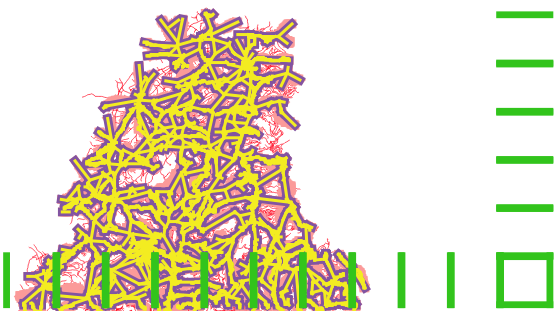
\includegraphics[angle=90]{Figures/Art/Capture d’écran 2016-08-08 à 11.46.55}


%%%%%%%%%%%%%%%%%%




% Q : model behavior to be put in the thesis or in metadata link to git repo ?
%  -> as code, unreadable directly : put listing of statistical analysis
% TODO : find a way to automatically generate stat anal files from R ?


%%%%%%%%%%%%%%%%%%
%% Appendix : models behavior ?
%\include{Appendices/Behavior}
%%%%%%%%%%%%%%%%%%


% TODO : companion site à la Seb ?

% TODO : a note on open review via git ?





%----------------------------------------------------------------------------------------
%	POST-CONTENT THESIS PAGES
%----------------------------------------------------------------------------------------


%\cleardoublepage% Declaration

\refstepcounter{dummy}
\pdfbookmark[0]{Declaration}{declaration} % Bookmark name visible in a PDF viewer

\chapter*{Declaration} % Declaration section text

\thispagestyle{empty}

Put your declaration here.
\bigskip
 
\noindent\textit{\myLocation, \myTime}

\smallskip

\begin{flushright}
\begin{tabular}{m{5cm}}
\\ \hline
\centering\myName \\
\end{tabular}
\end{flushright}
 % Declaration

%\cleardoublepage% Colophon (a brief description of publication or production notes relevant to the edition)

\pagestyle{empty}

\hfill

\vfill

\pdfbookmark[0]{Colophon}{colophon}

\section*{Colophon}

This document was typeset using the typographical look-and-feel \texttt{classicthesis} developed by Andr\'e Miede. The style was inspired by Robert Bringhurst's seminal book on typography ``\emph{The Elements of Typographic Style}''. \texttt{classicthesis} is available for both \LaTeX\ and \mLyX: 

\begin{center}
\url{https://bitbucket.org/amiede/classicthesis/}
\end{center}

\noindent Happy users of \texttt{classicthesis} usually send a real postcard to the author, a collection of postcards received so far is featured here: 

\begin{center}
\url{http://postcards.miede.de/}
\end{center}
 
\bigskip

\noindent\finalVersionString % Colophon

%----------------------------------------------------------------------------------------

\end{document}
